\documentclass{article}
\usepackage{graphicx}
\usepackage[margin=1cm]{geometry}
\usepackage{amsmath}
\pagenumbering{gobble}
\begin{document}
\setlength\parindent{0pt}
\begin{verbatim}
more than one reactant
fragment matching found
free_energy dG is above threshold=0.0
Terminal.KEEP
\end{verbatim}
$$
69
\raisebox{-.5\height}{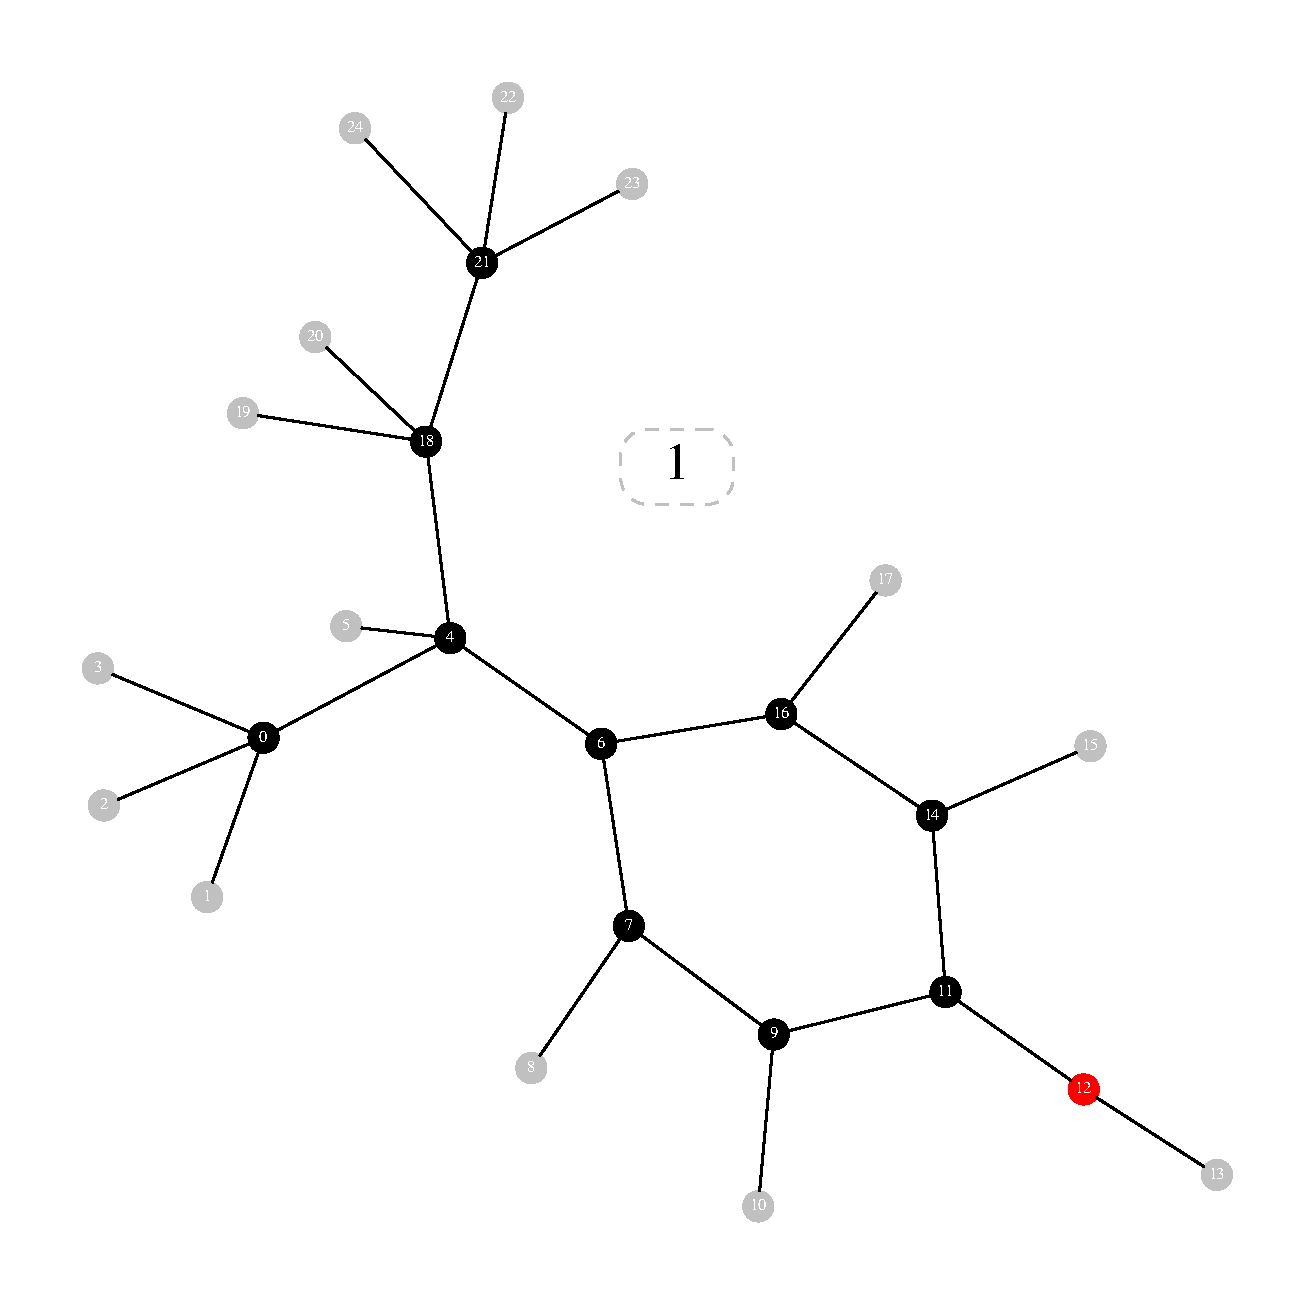
\includegraphics[scale=0.15]{mol_pictures/69.pdf}}
+
87
\raisebox{-.5\height}{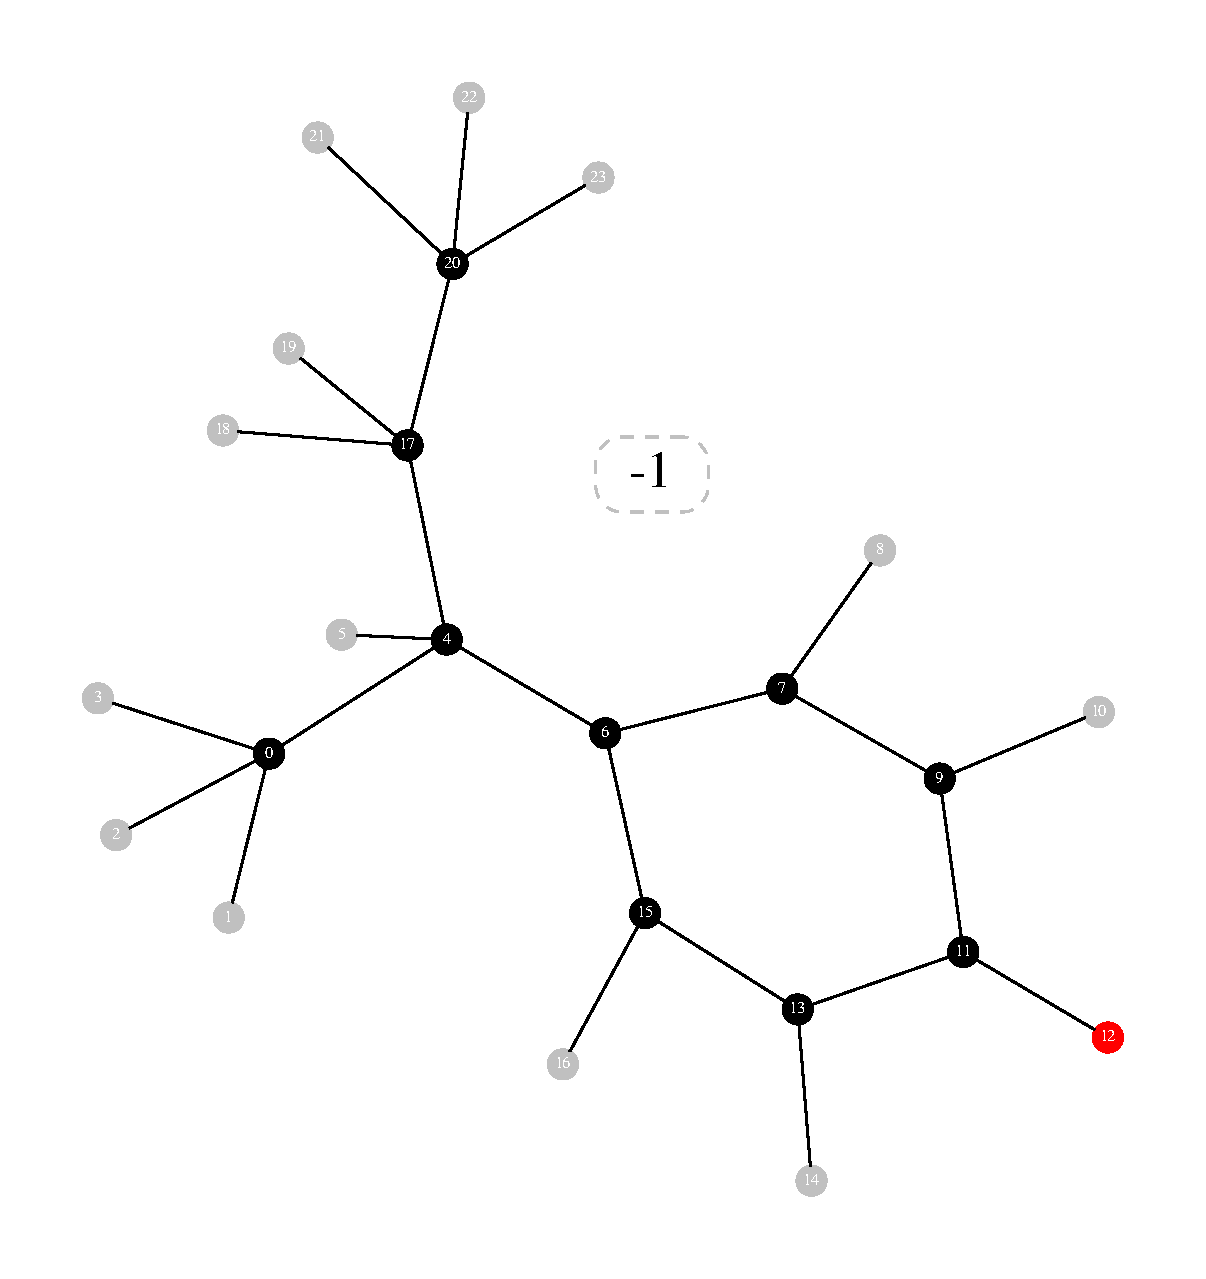
\includegraphics[scale=0.15]{mol_pictures/87.pdf}}
\xrightarrow[0.23]{2.26}
66
\raisebox{-.5\height}{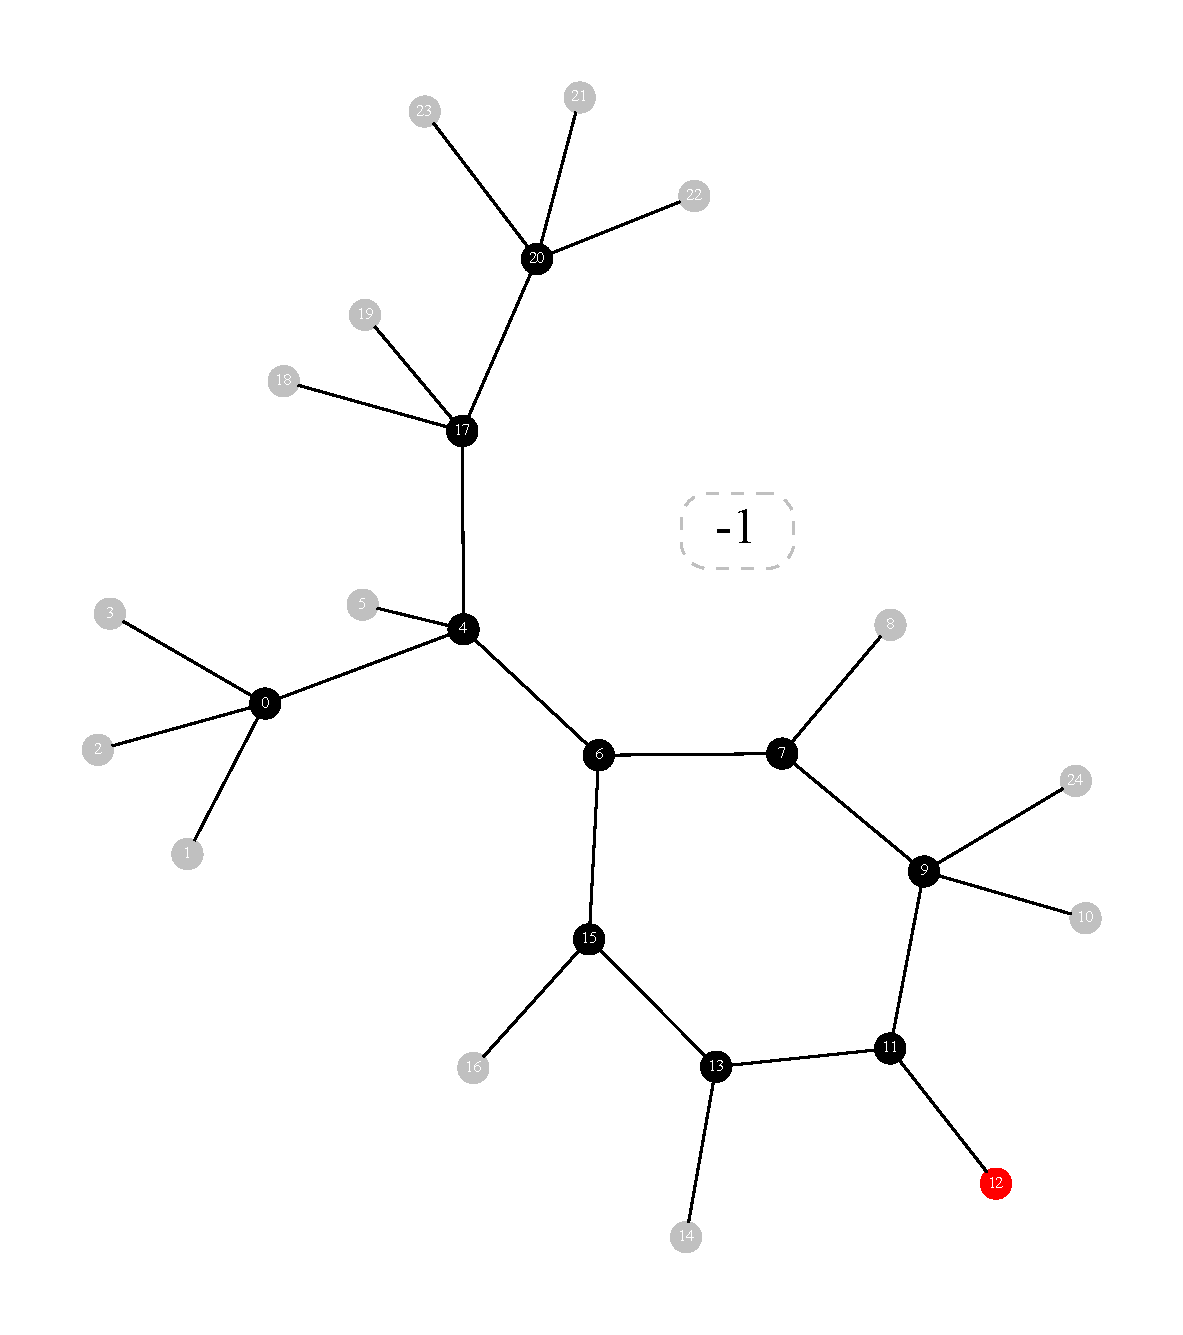
\includegraphics[scale=0.15]{mol_pictures/66.pdf}}
+
89
\raisebox{-.5\height}{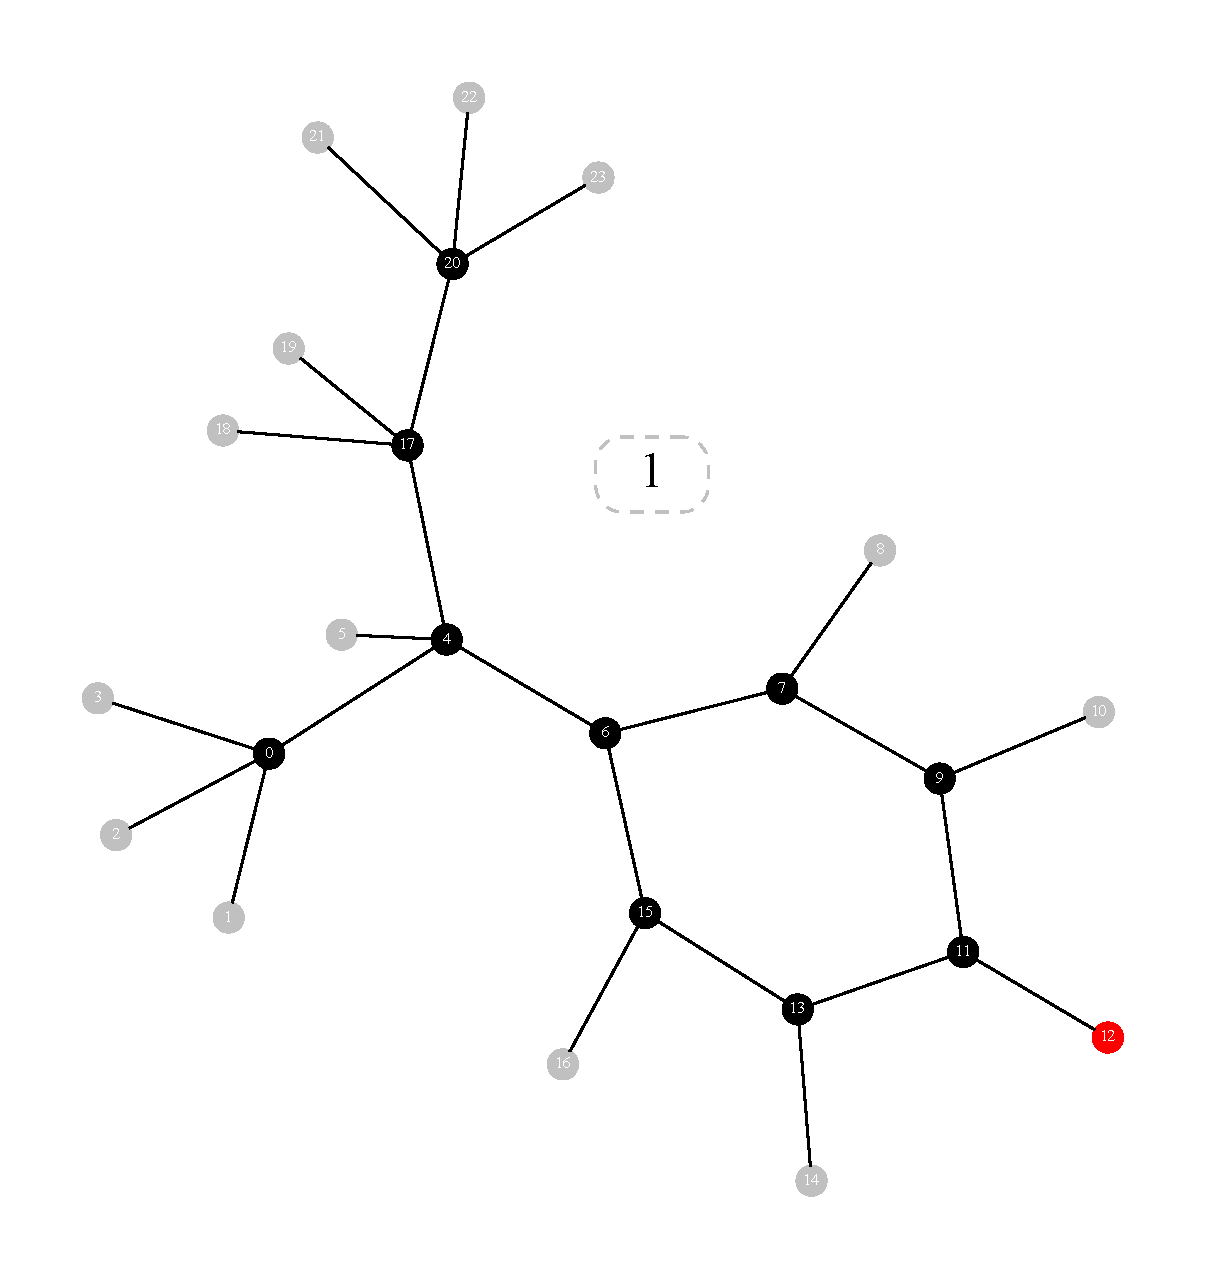
\includegraphics[scale=0.15]{mol_pictures/89.pdf}}
$$


reactant bonds broken:\begin{verbatim}
[(0, 12), (0, 13)]
\end{verbatim}
product bonds broken:\begin{verbatim}
[(0, 9), (0, 10)]
\end{verbatim}




\vspace{1cm}
\begin{verbatim}
more than one reactant
fragment matching found
free_energy dG is above threshold=0.0
Terminal.KEEP
\end{verbatim}
$$
69
\raisebox{-.5\height}{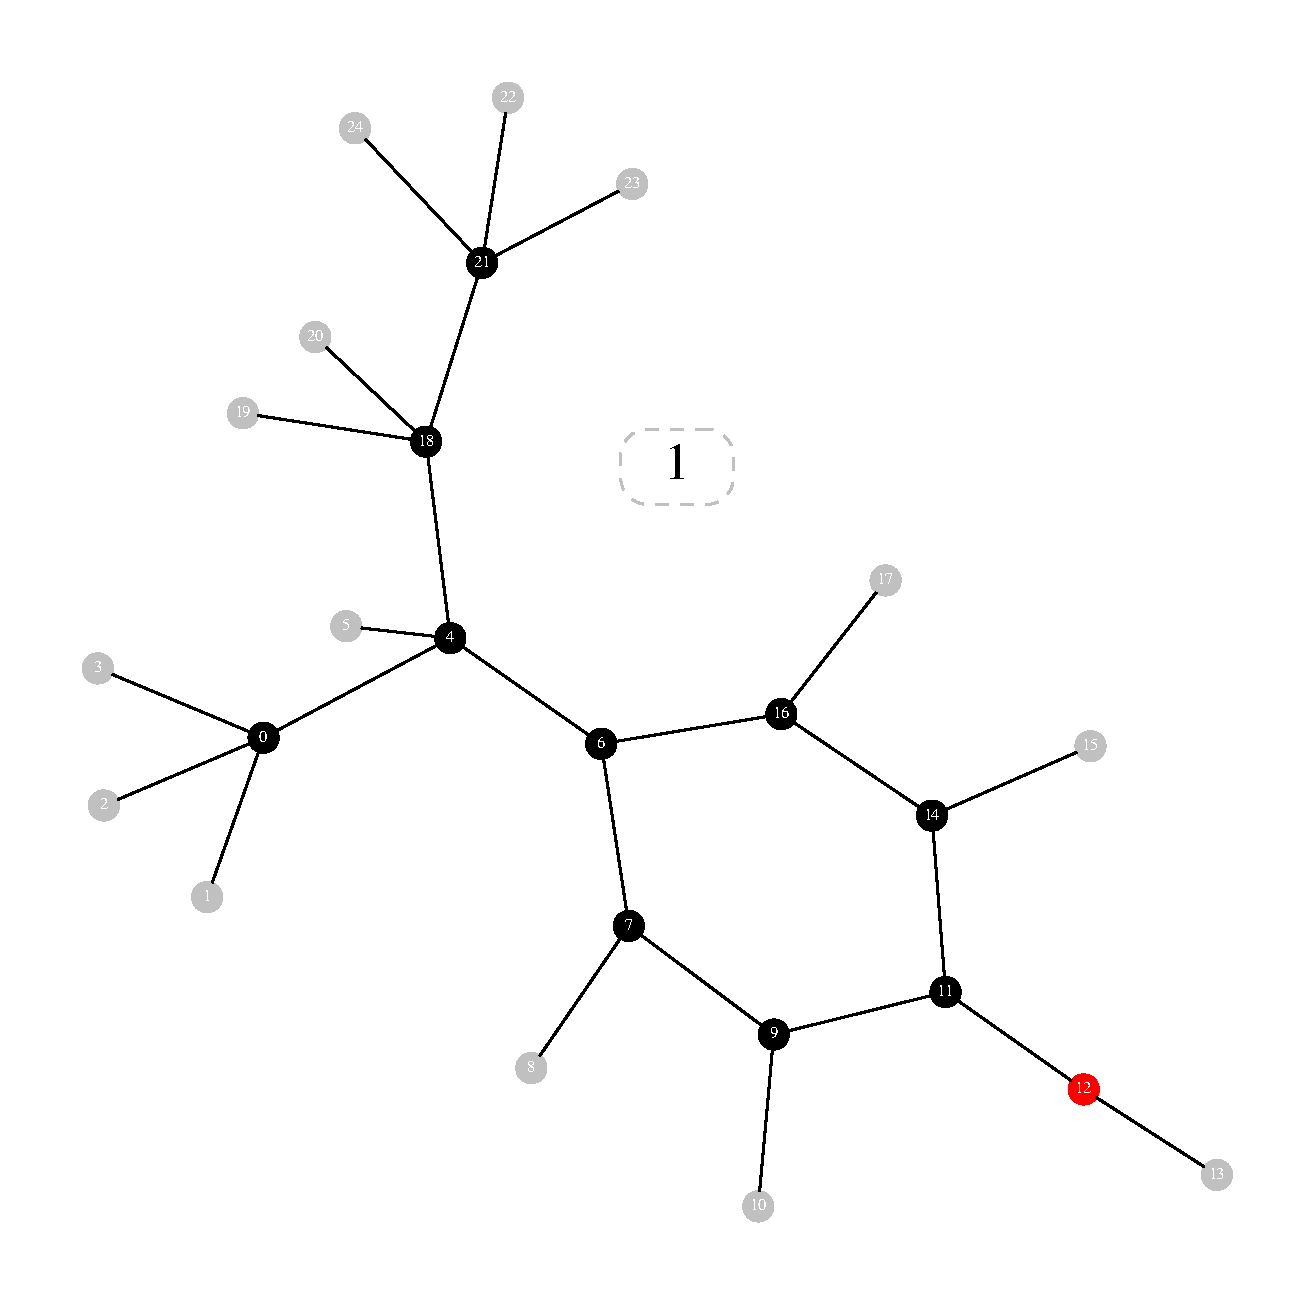
\includegraphics[scale=0.15]{mol_pictures/69.pdf}}
+
88
\raisebox{-.5\height}{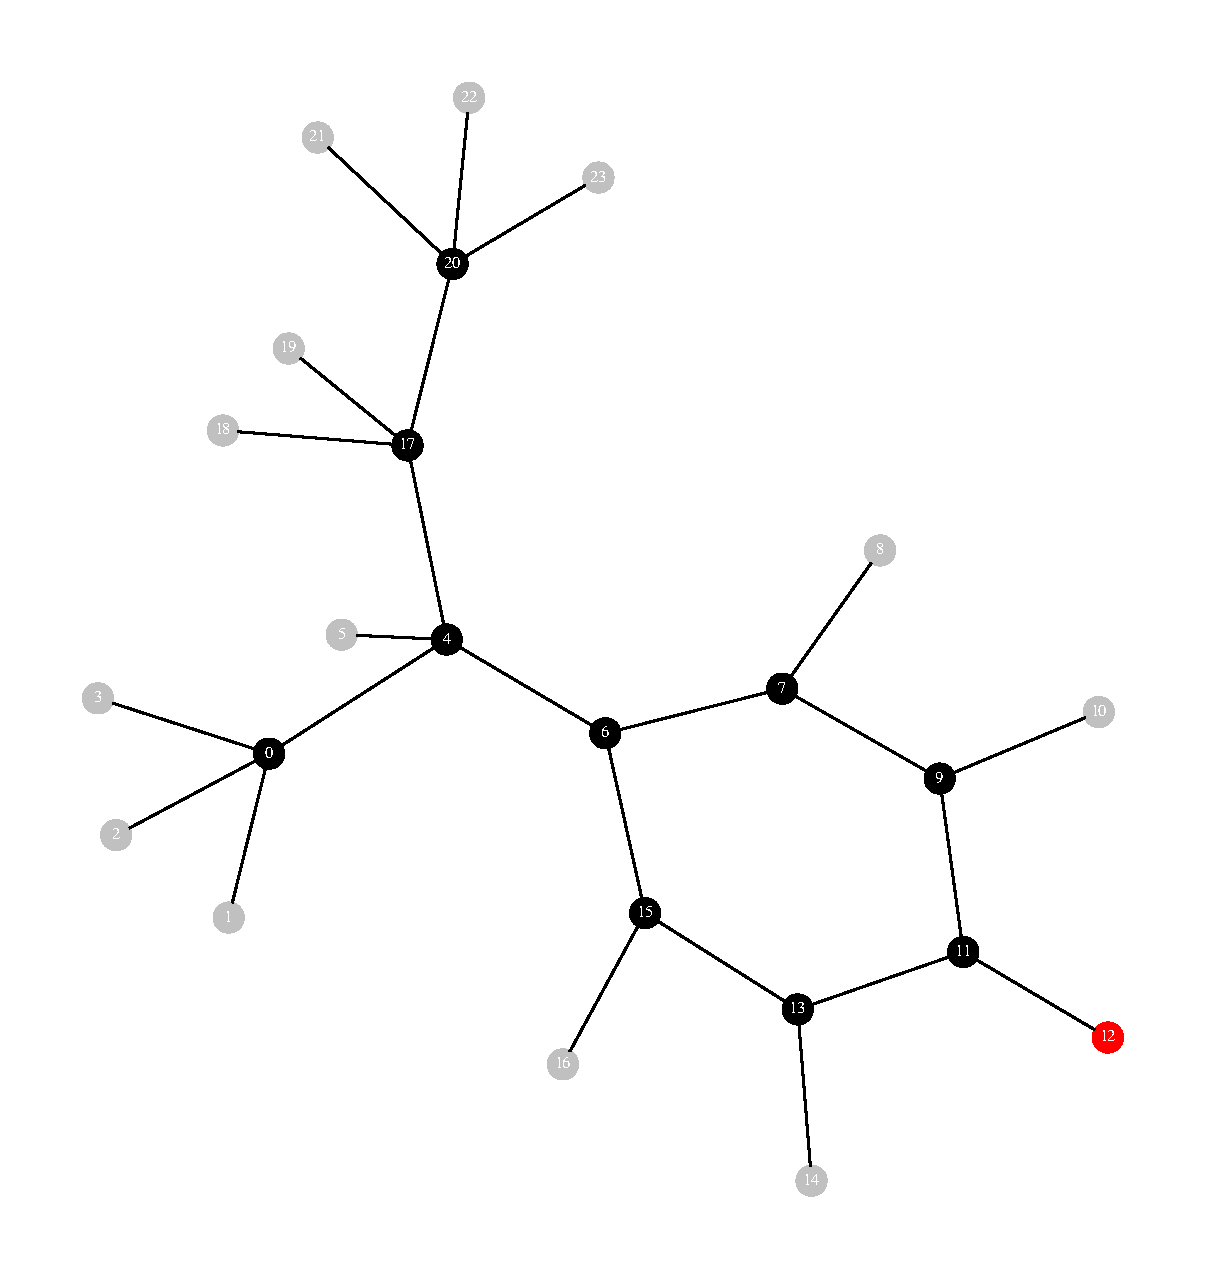
\includegraphics[scale=0.15]{mol_pictures/88.pdf}}
\xrightarrow[0.00]{0.05}
67
\raisebox{-.5\height}{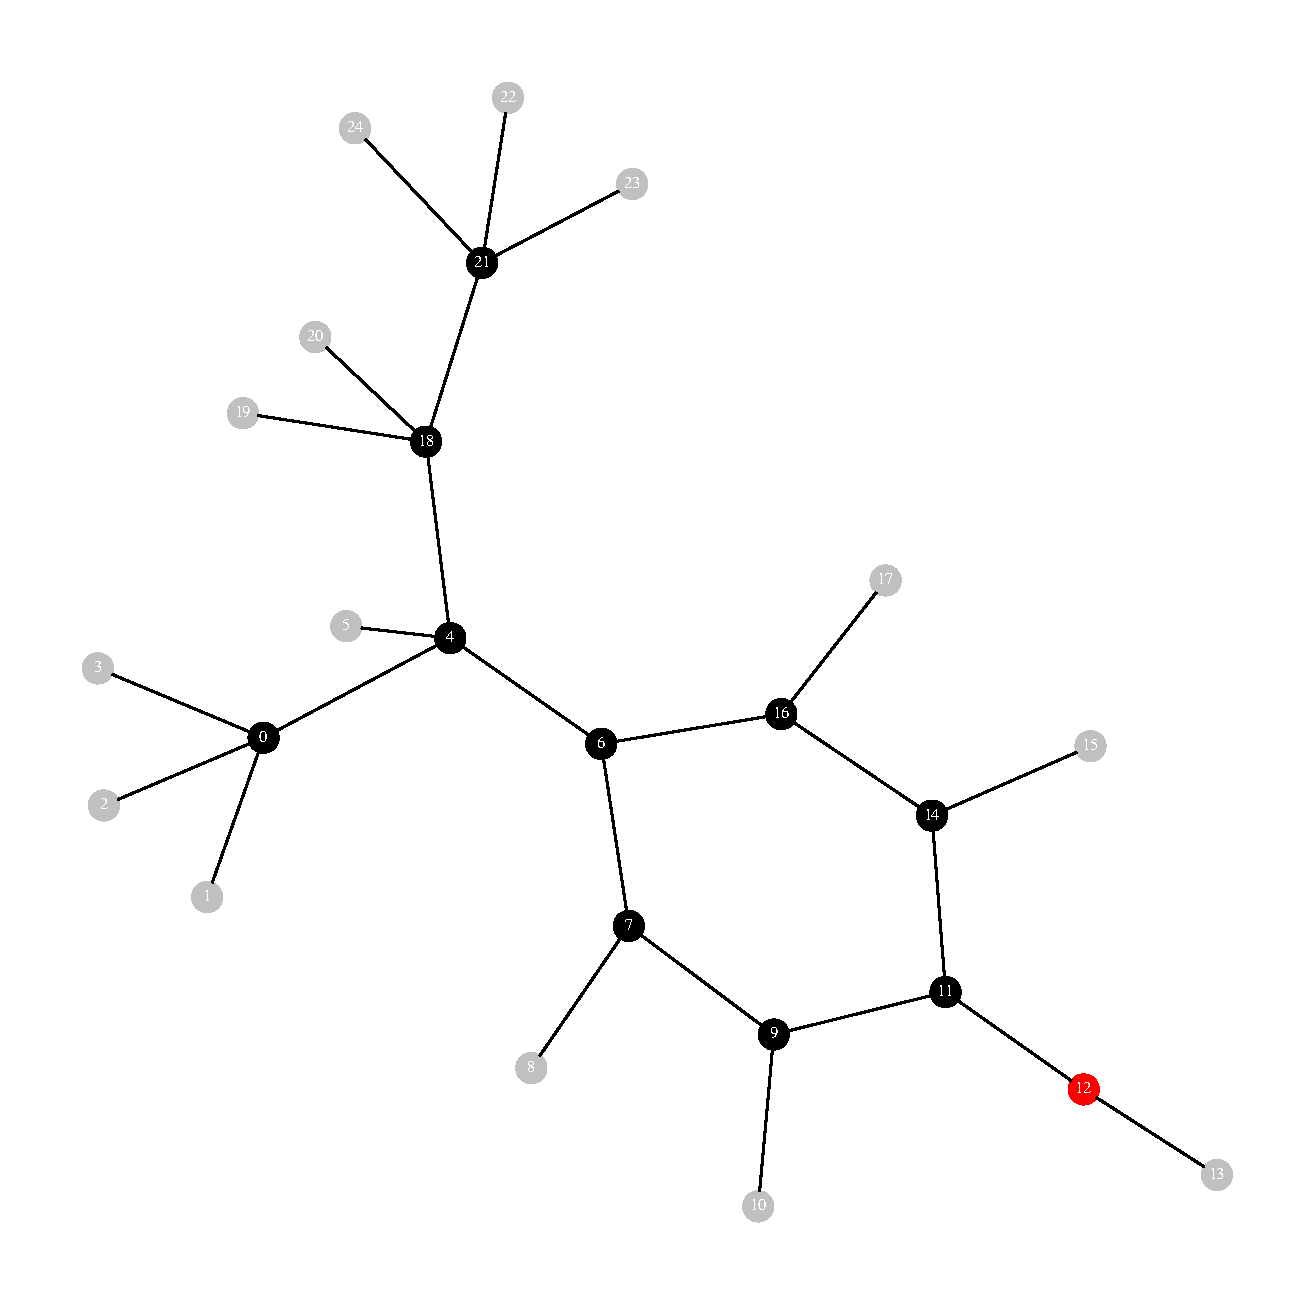
\includegraphics[scale=0.15]{mol_pictures/67.pdf}}
+
89
\raisebox{-.5\height}{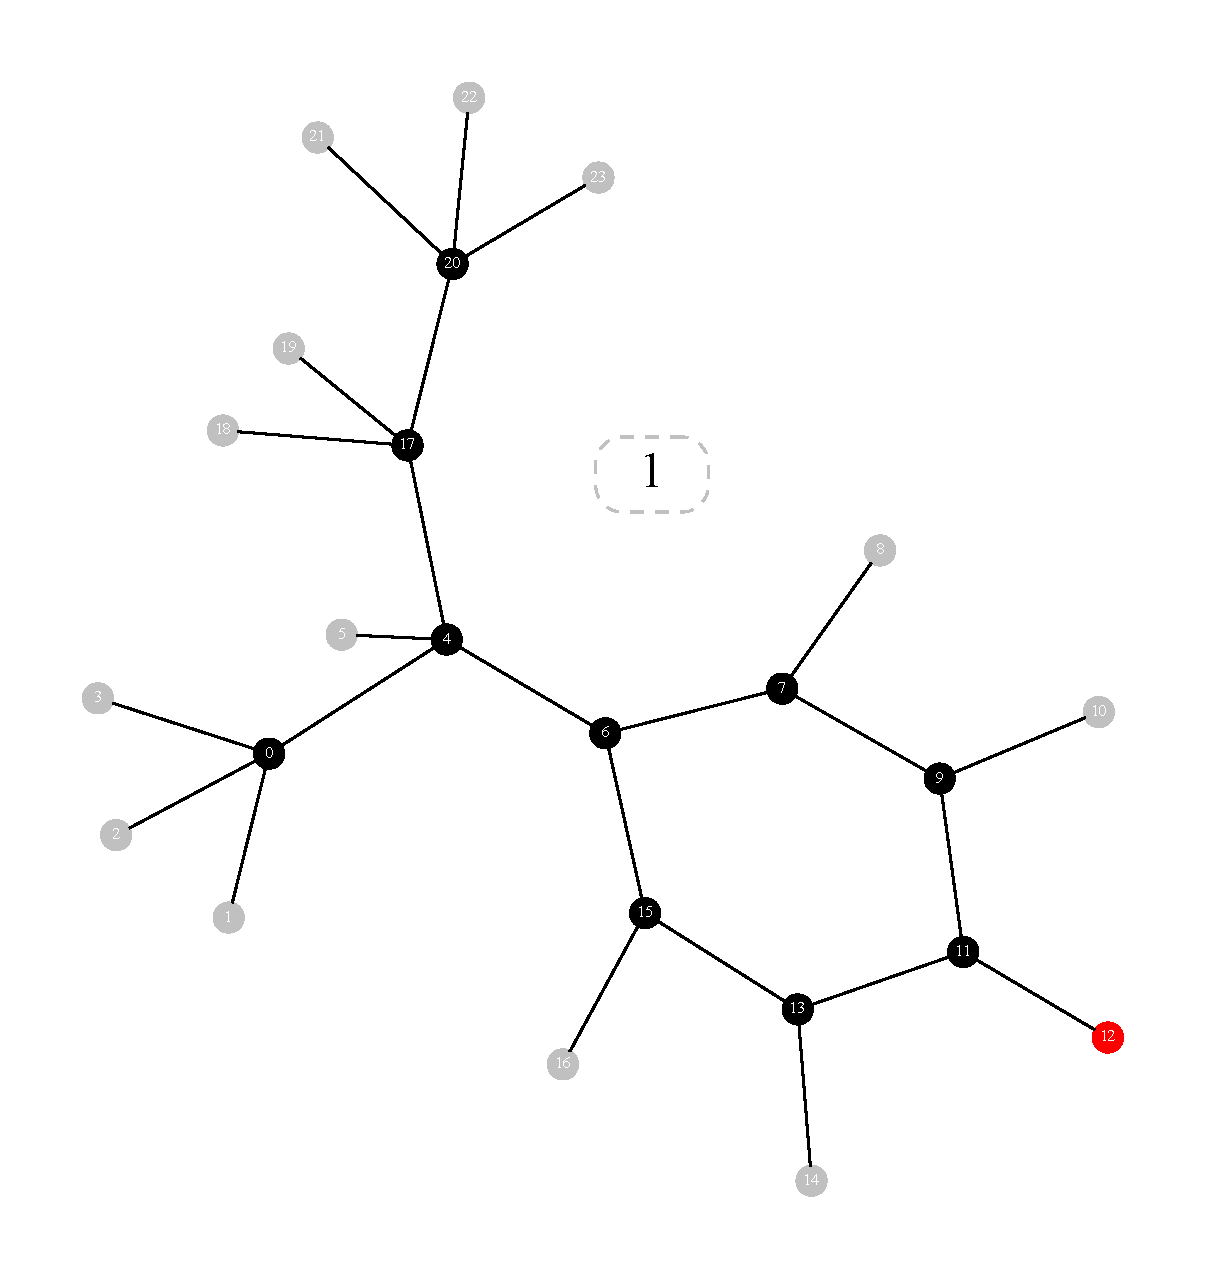
\includegraphics[scale=0.15]{mol_pictures/89.pdf}}
$$


reactant bonds broken:\begin{verbatim}
[(1, 0), (1, 3)]
\end{verbatim}
product bonds broken:\begin{verbatim}
[(1, 0), (1, 3)]
\end{verbatim}




\vspace{1cm}
\begin{verbatim}
more than one reactant
fragment matching found
free_energy dG is above threshold=0.0
Terminal.KEEP
\end{verbatim}
$$
69
\raisebox{-.5\height}{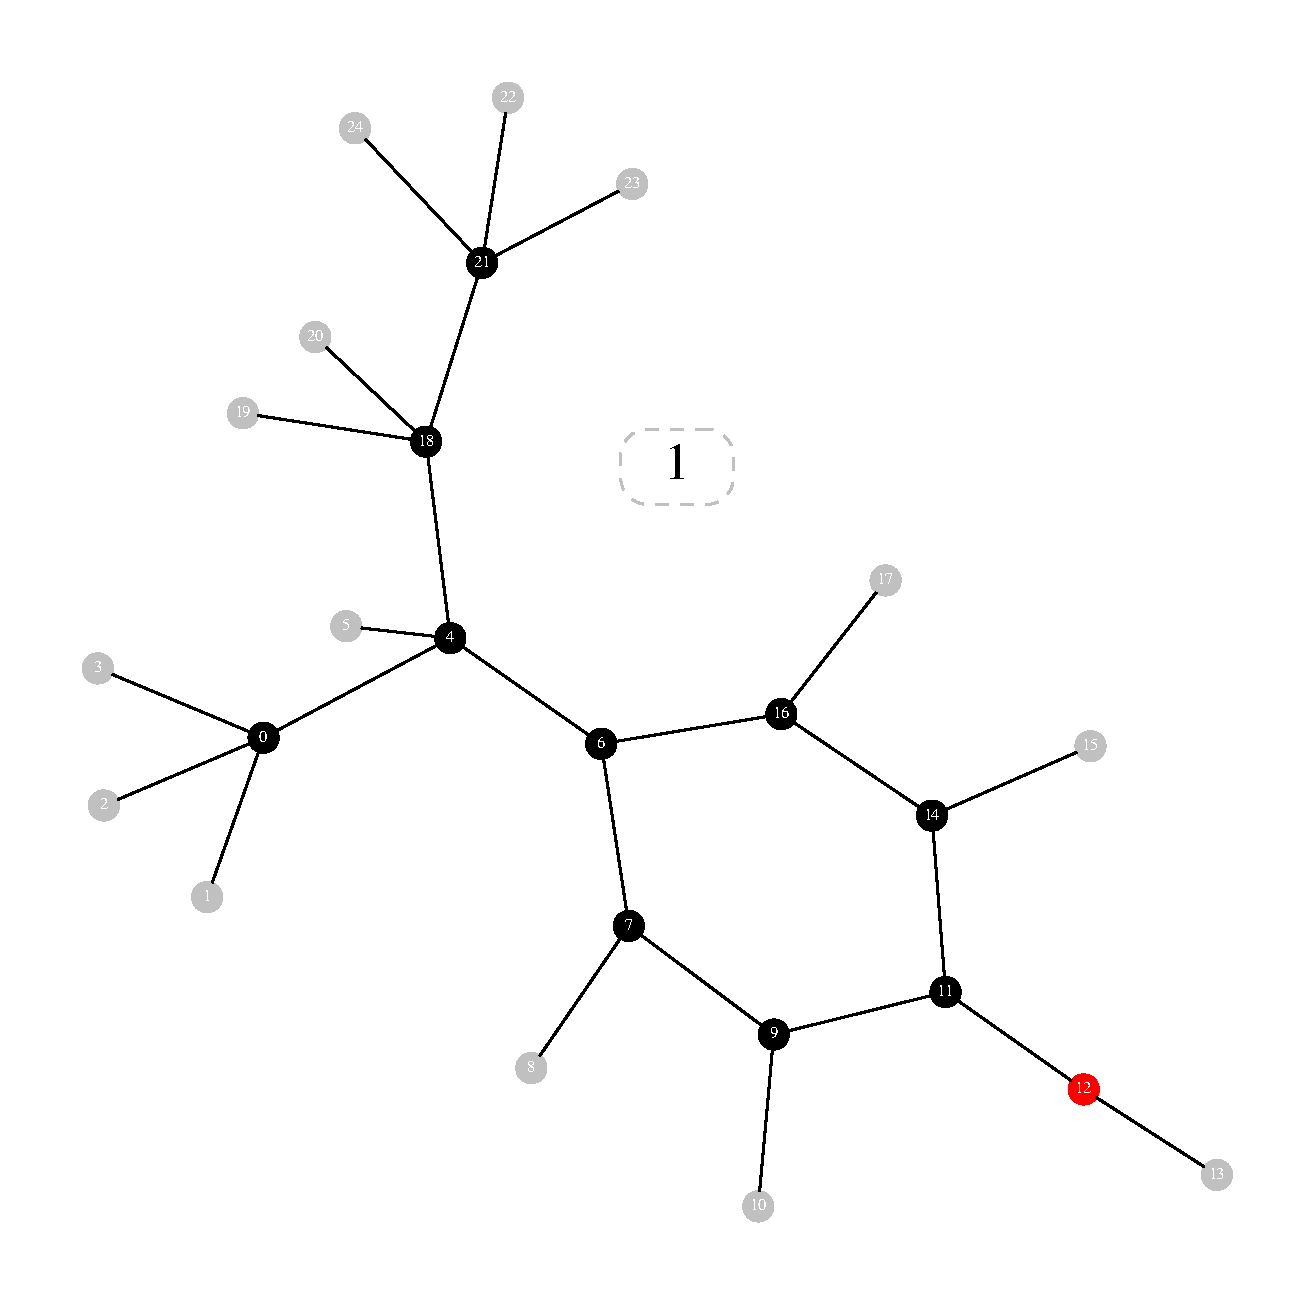
\includegraphics[scale=0.15]{mol_pictures/69.pdf}}
+
88
\raisebox{-.5\height}{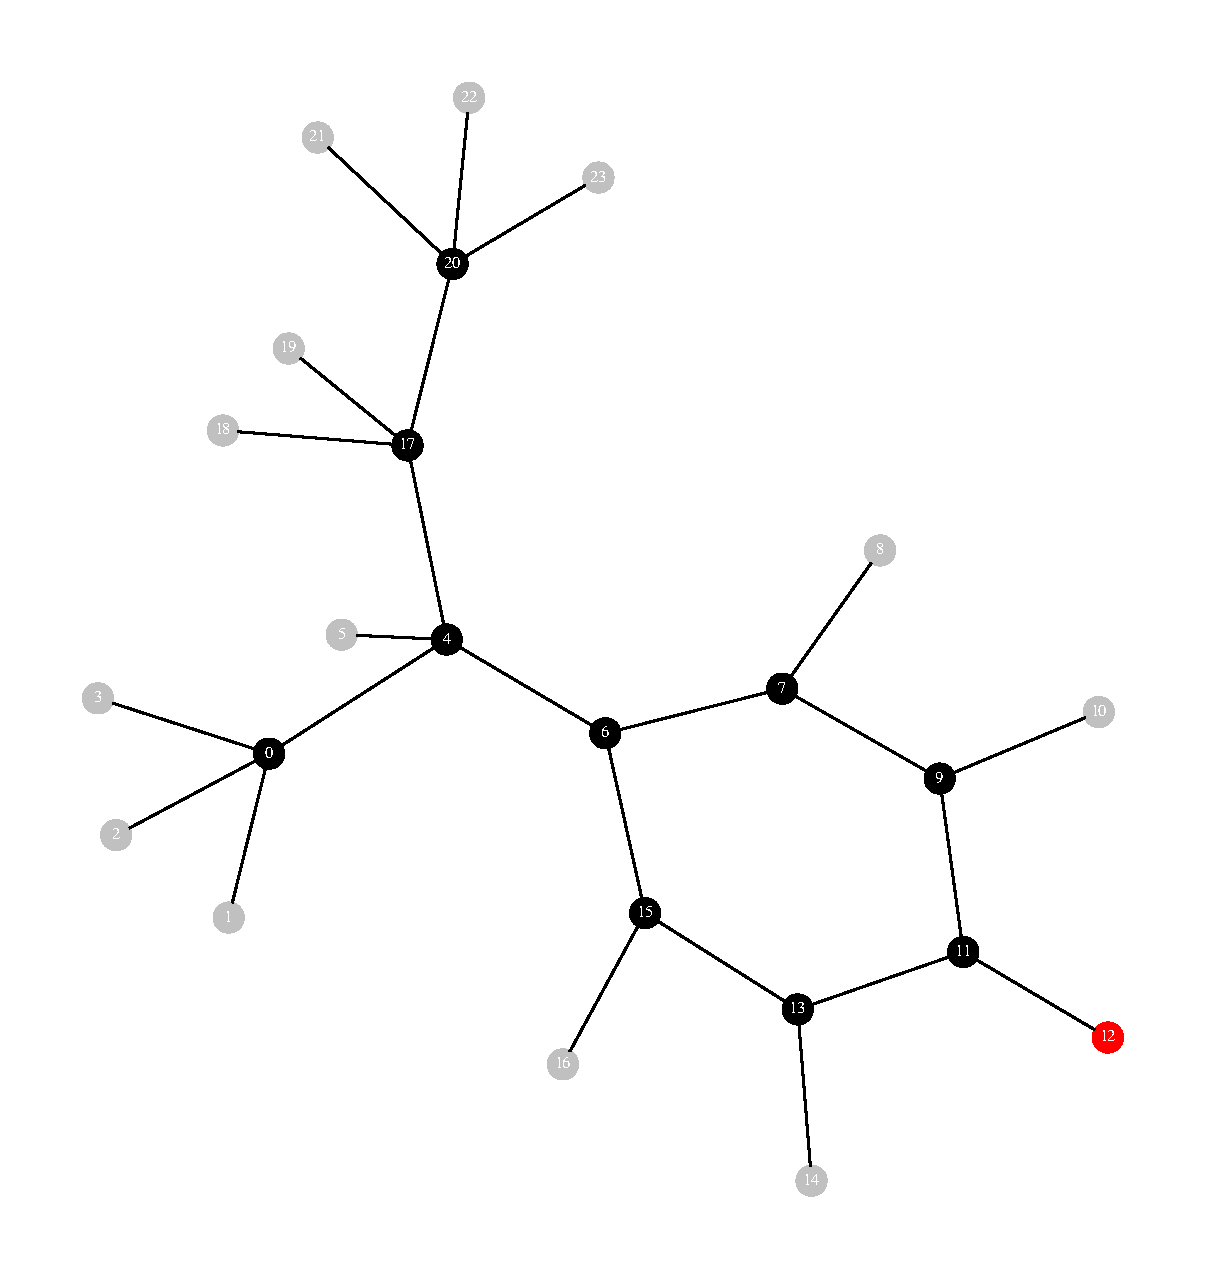
\includegraphics[scale=0.15]{mol_pictures/88.pdf}}
\xrightarrow[0.07]{0.73}
68
\raisebox{-.5\height}{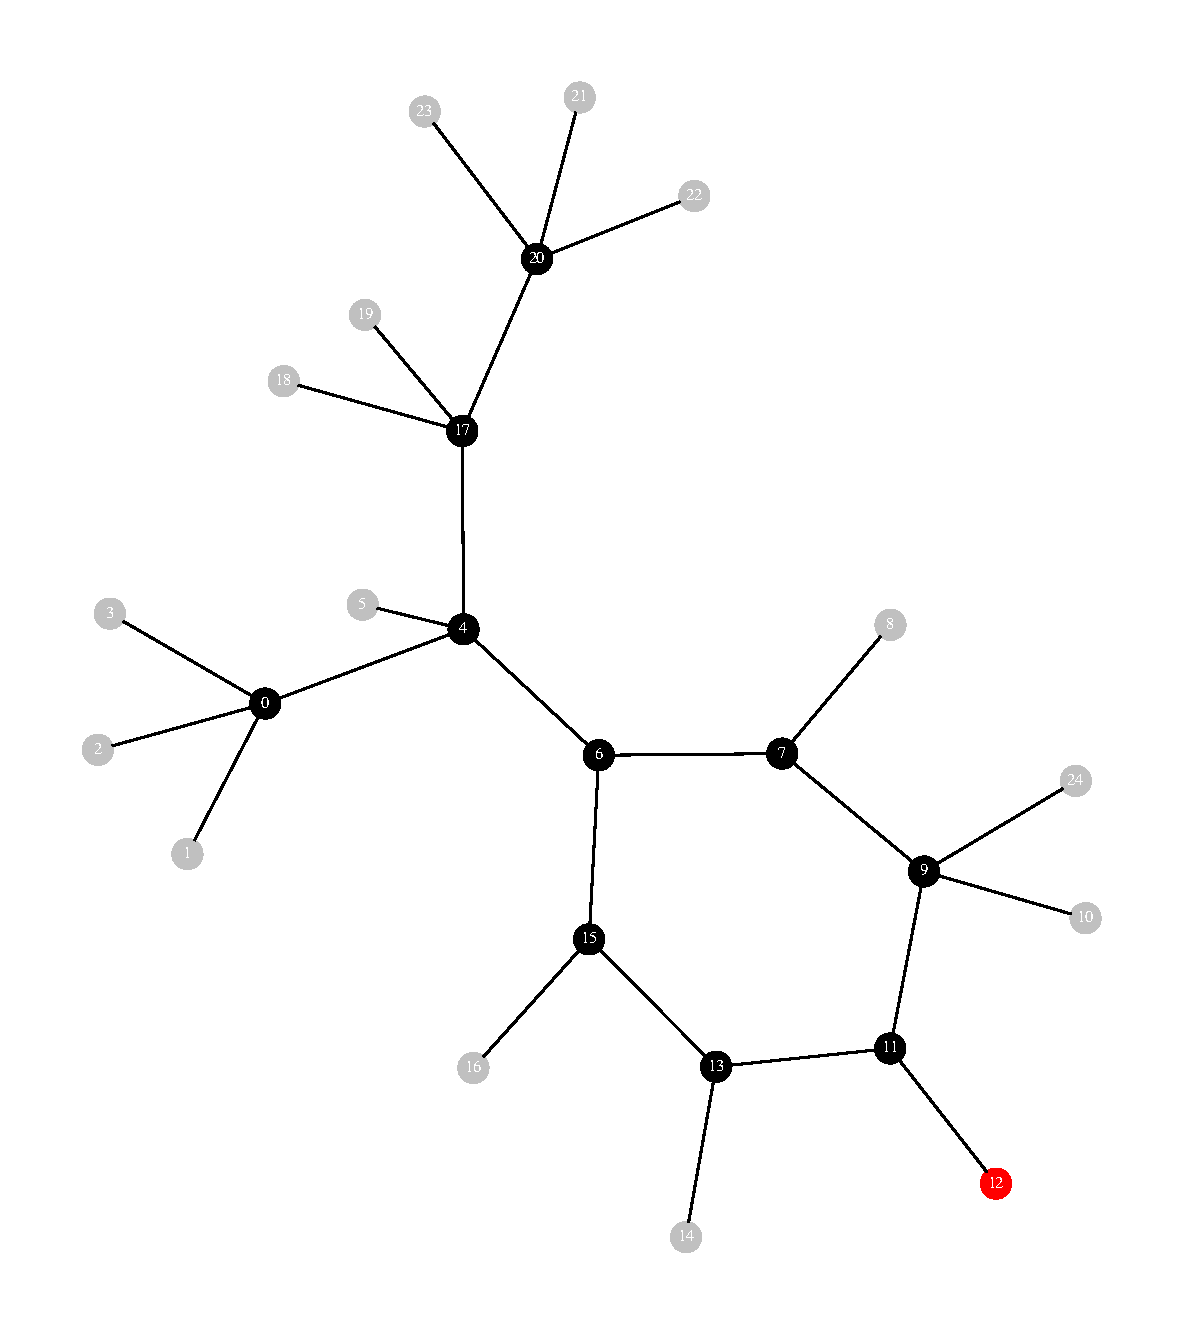
\includegraphics[scale=0.15]{mol_pictures/68.pdf}}
+
89
\raisebox{-.5\height}{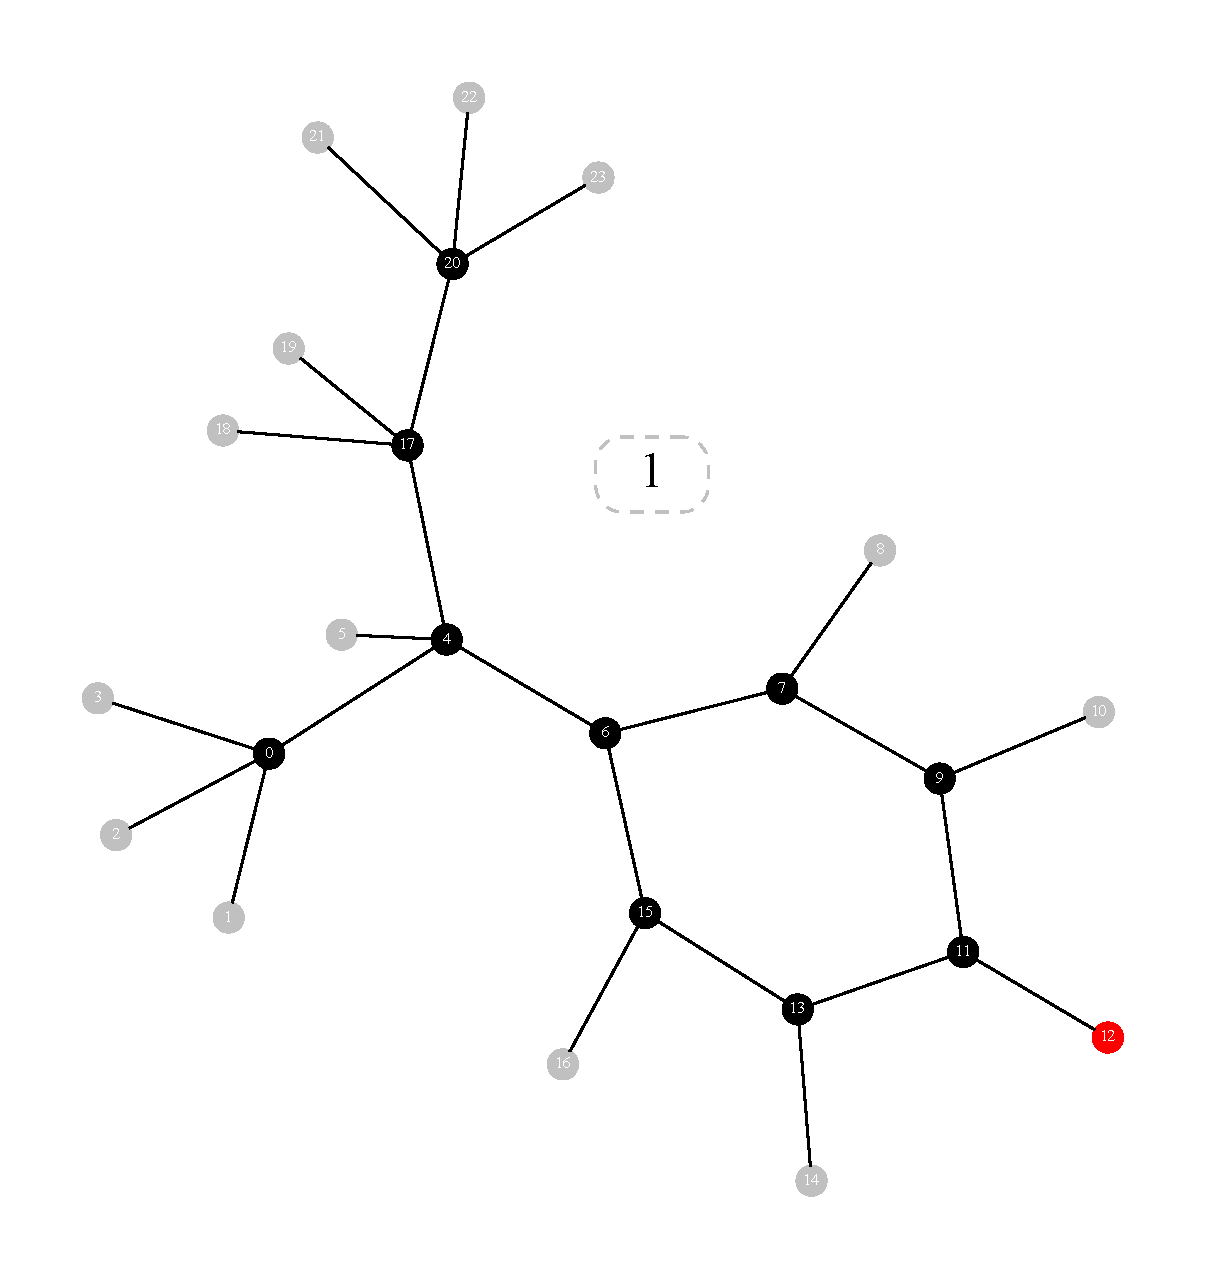
\includegraphics[scale=0.15]{mol_pictures/89.pdf}}
$$


reactant bonds broken:\begin{verbatim}
[(0, 12), (0, 13)]
\end{verbatim}
product bonds broken:\begin{verbatim}
[(0, 9), (0, 10)]
\end{verbatim}




\vspace{1cm}
\begin{verbatim}
more than one reactant
fragment matching found
free_energy dG is above threshold=0.0
Terminal.KEEP
\end{verbatim}
$$
70
\raisebox{-.5\height}{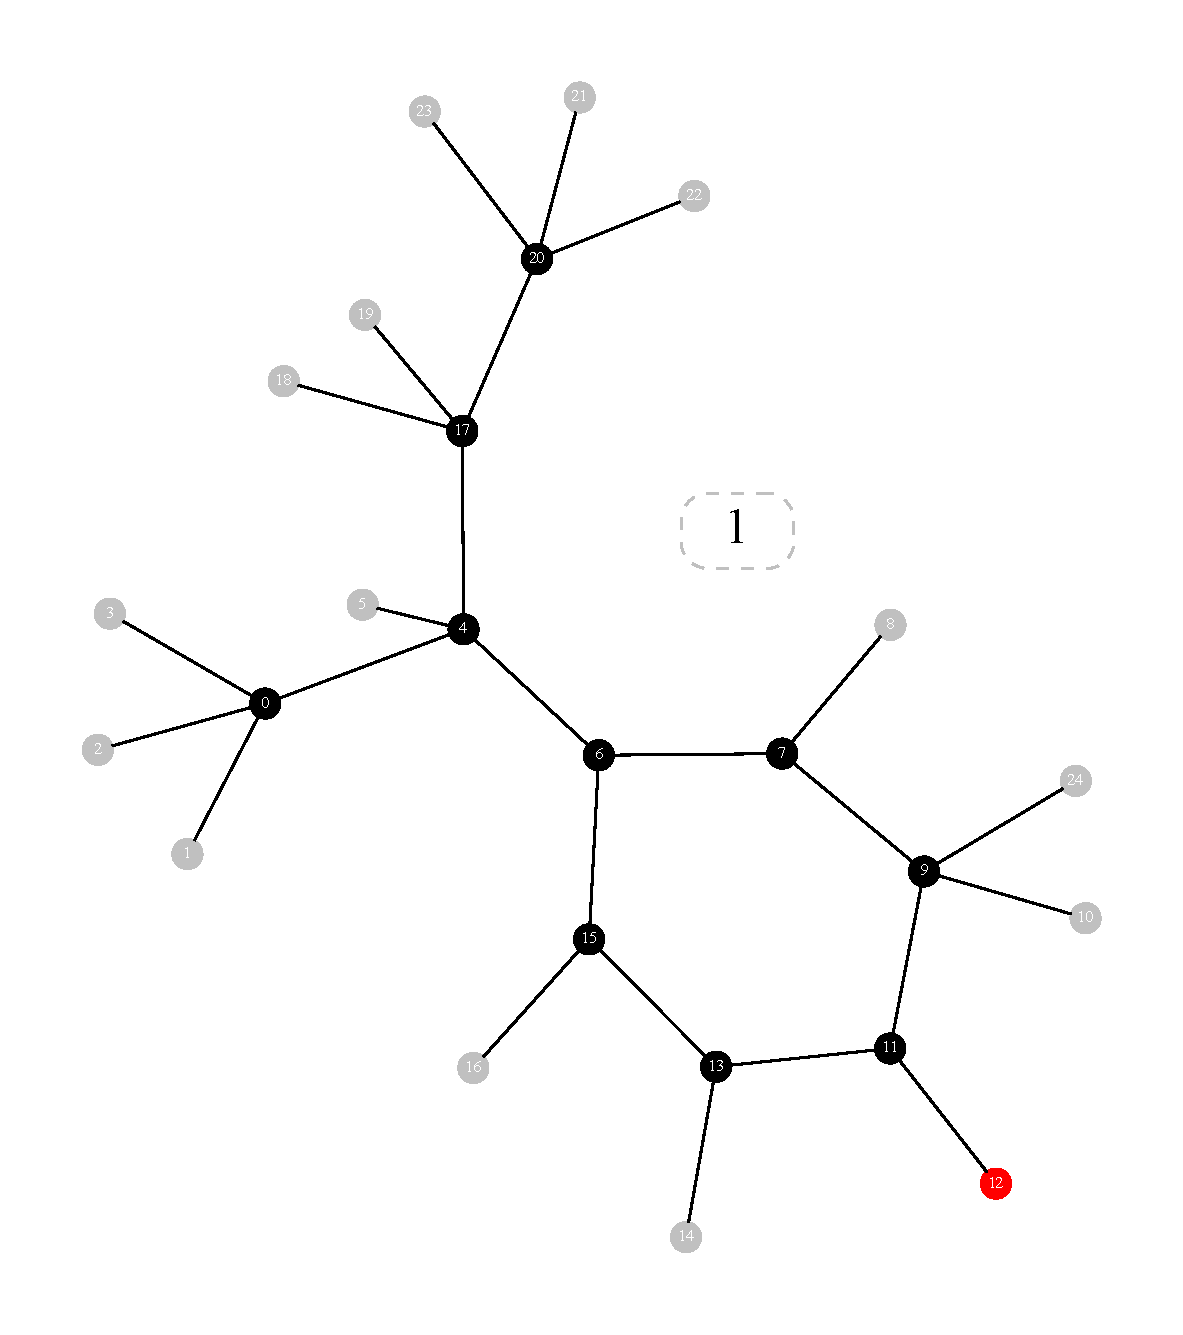
\includegraphics[scale=0.15]{mol_pictures/70.pdf}}
+
87
\raisebox{-.5\height}{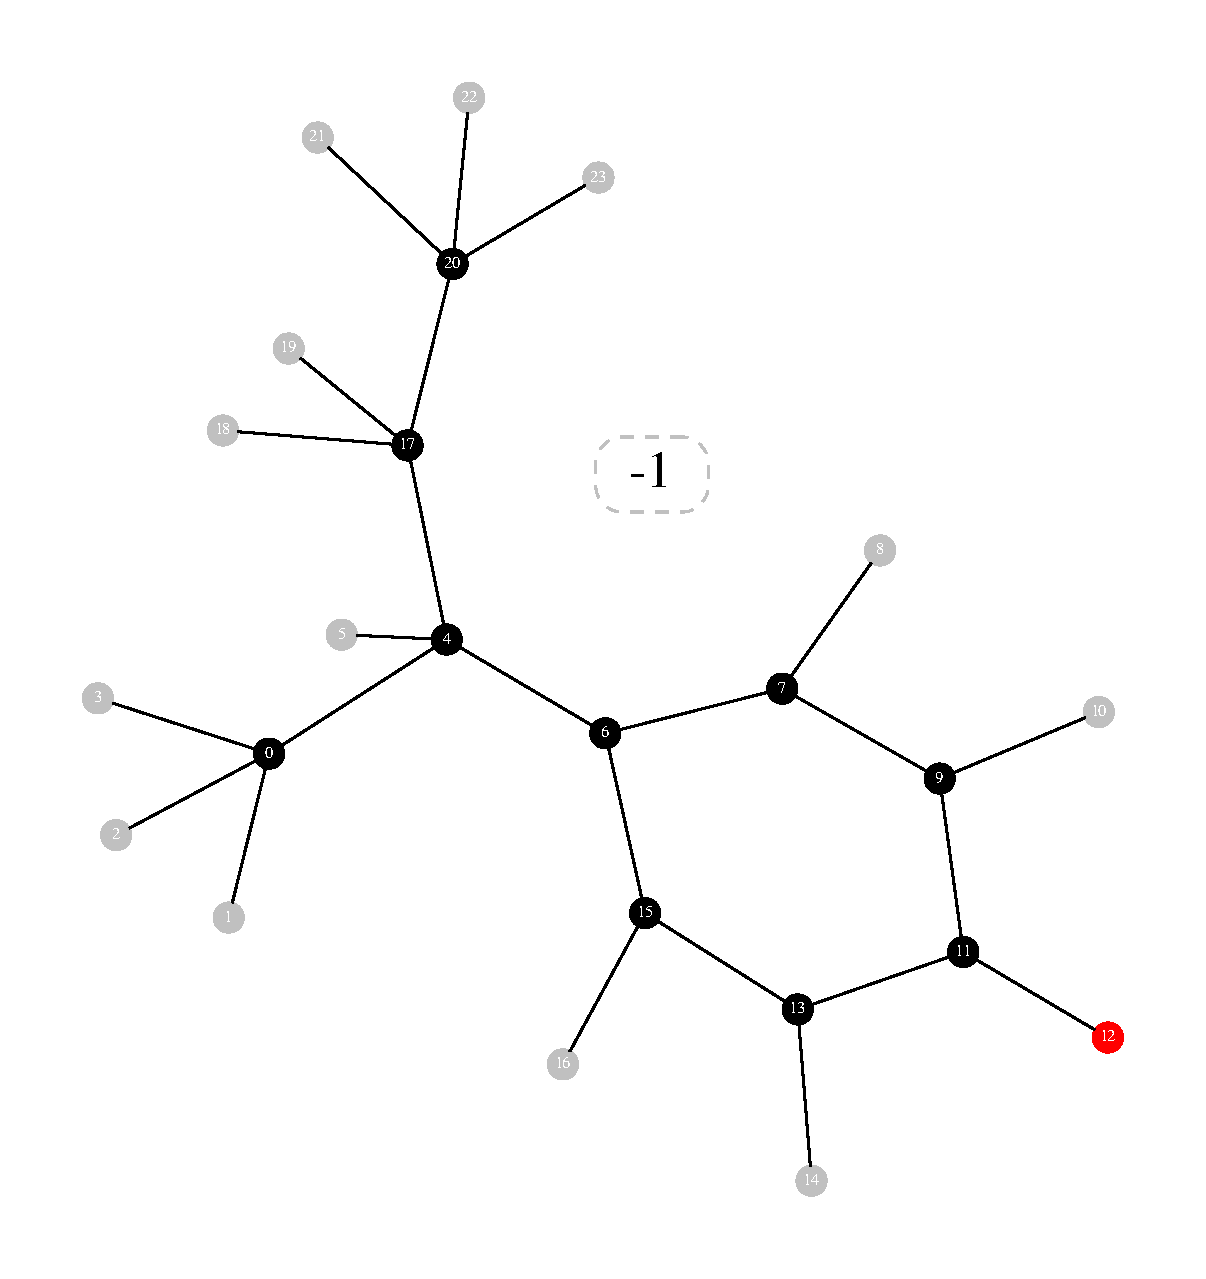
\includegraphics[scale=0.15]{mol_pictures/87.pdf}}
\xrightarrow[0.19]{1.94}
65
\raisebox{-.5\height}{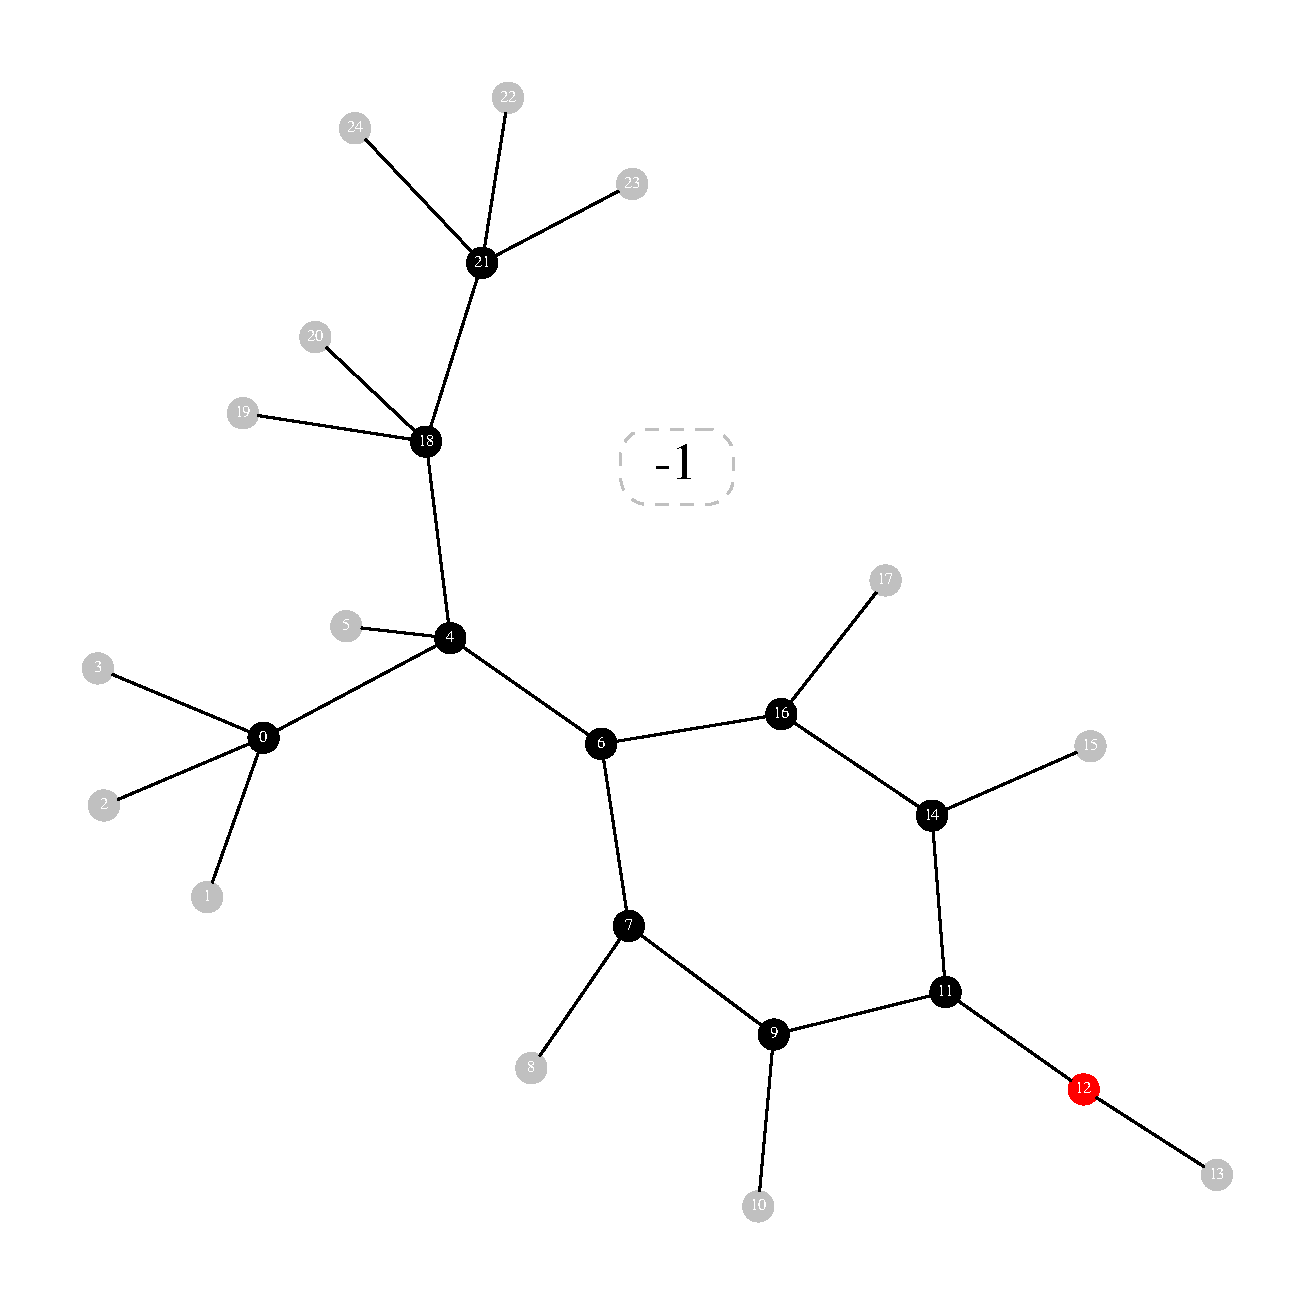
\includegraphics[scale=0.15]{mol_pictures/65.pdf}}
+
89
\raisebox{-.5\height}{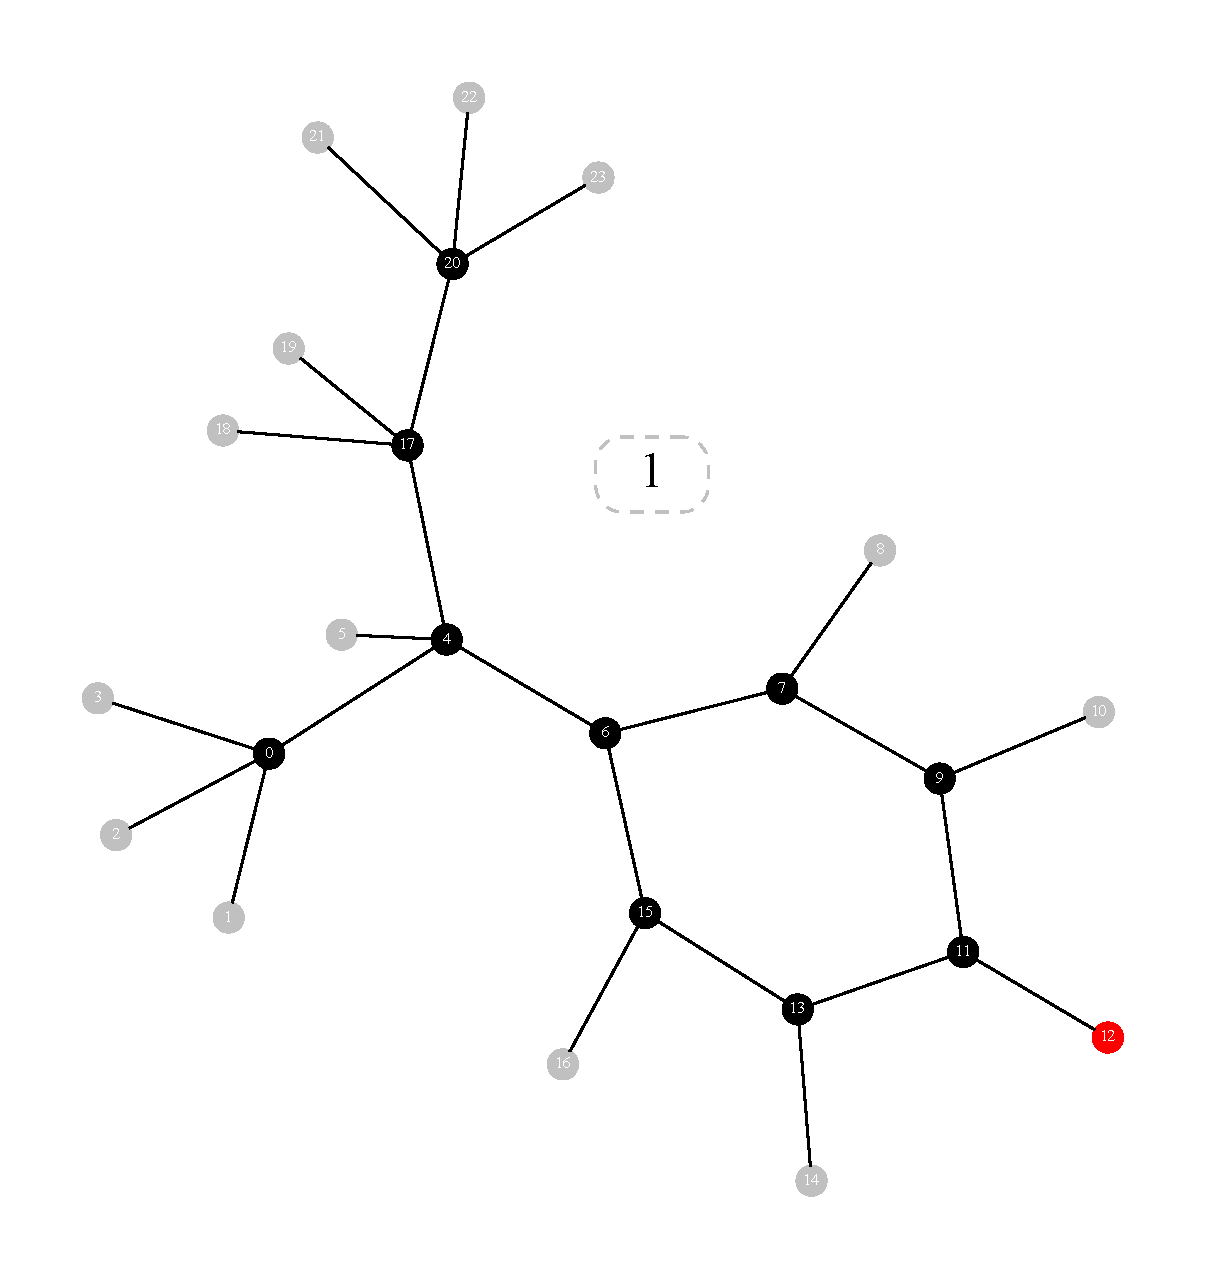
\includegraphics[scale=0.15]{mol_pictures/89.pdf}}
$$


reactant bonds broken:\begin{verbatim}
[(0, 9), (0, 10)]
\end{verbatim}
product bonds broken:\begin{verbatim}
[(0, 12), (0, 13)]
\end{verbatim}




\vspace{1cm}
\begin{verbatim}
more than one reactant
fragment matching found
free_energy dG is above threshold=0.0
Terminal.KEEP
\end{verbatim}
$$
54
\raisebox{-.5\height}{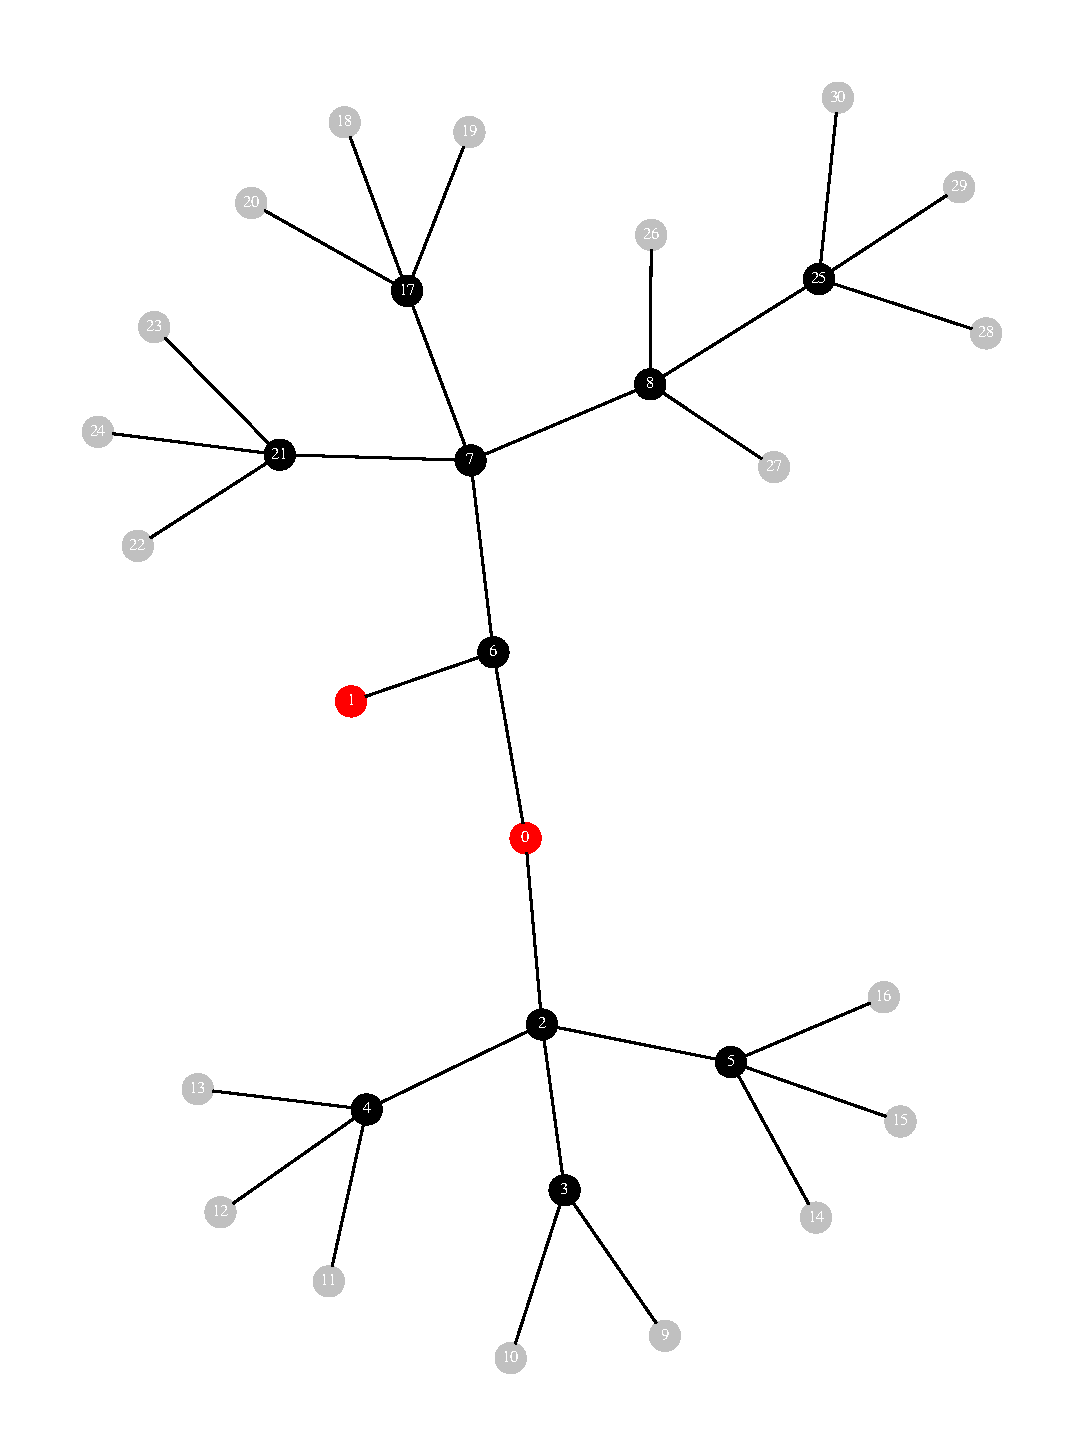
\includegraphics[scale=0.15]{mol_pictures/54.pdf}}
+
69
\raisebox{-.5\height}{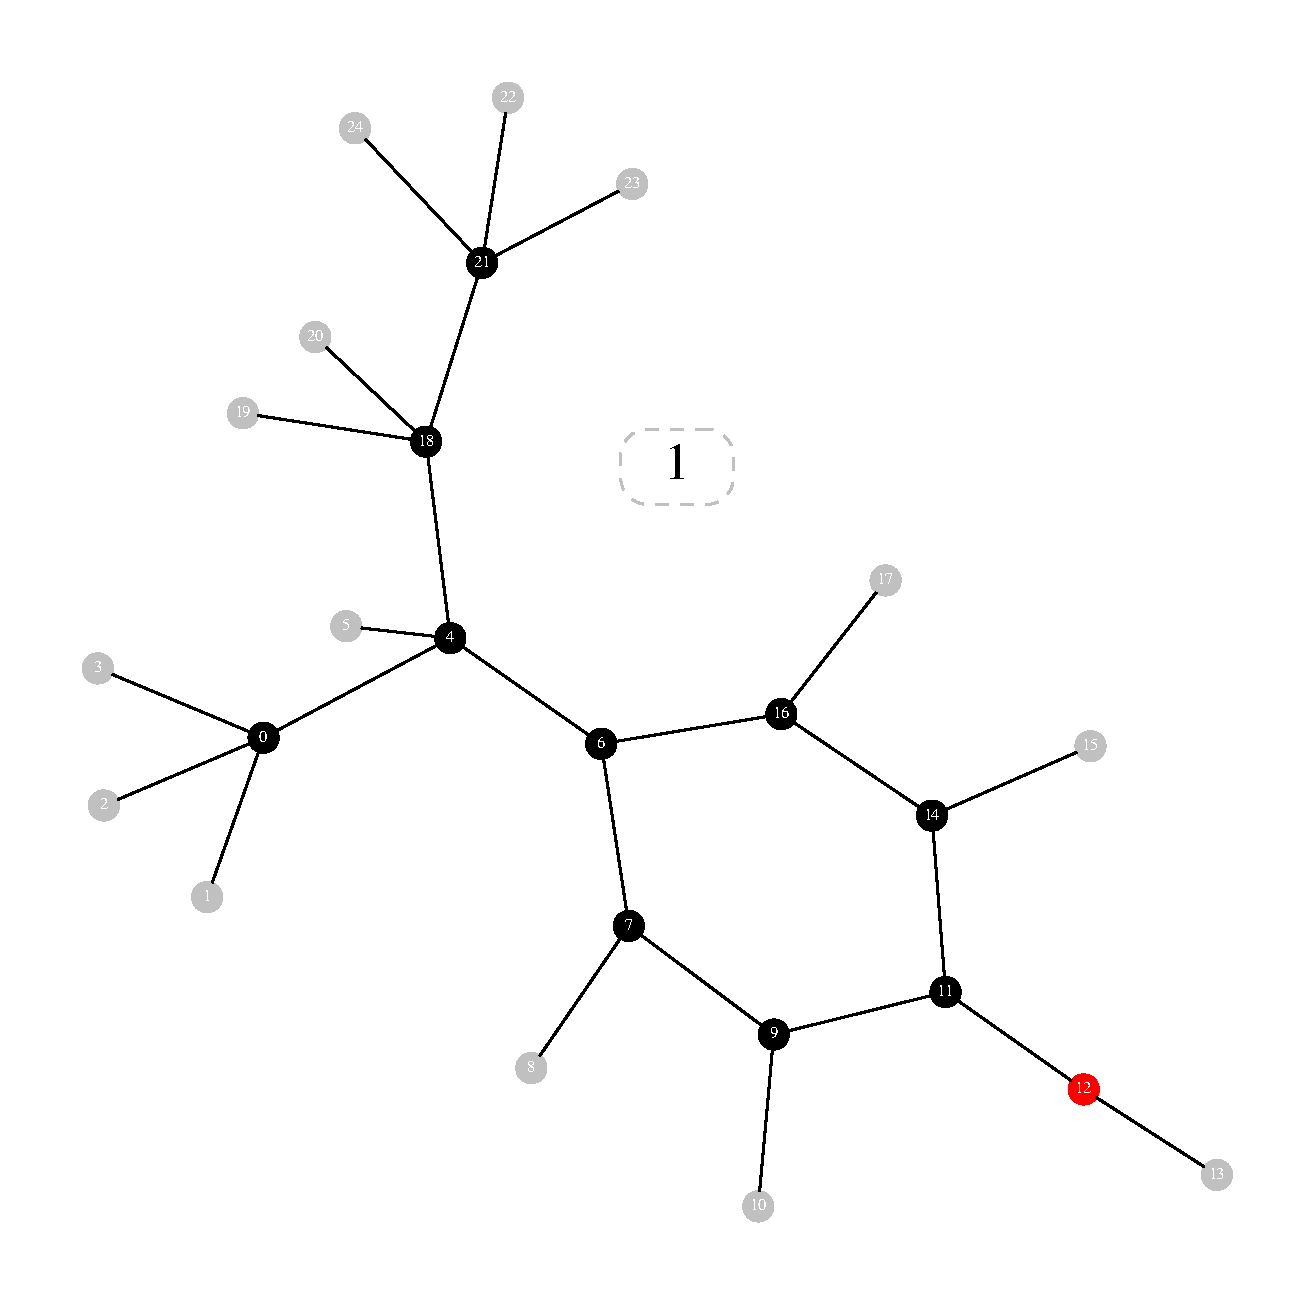
\includegraphics[scale=0.15]{mol_pictures/69.pdf}}
\xrightarrow[0.06]{0.60}
73
\raisebox{-.5\height}{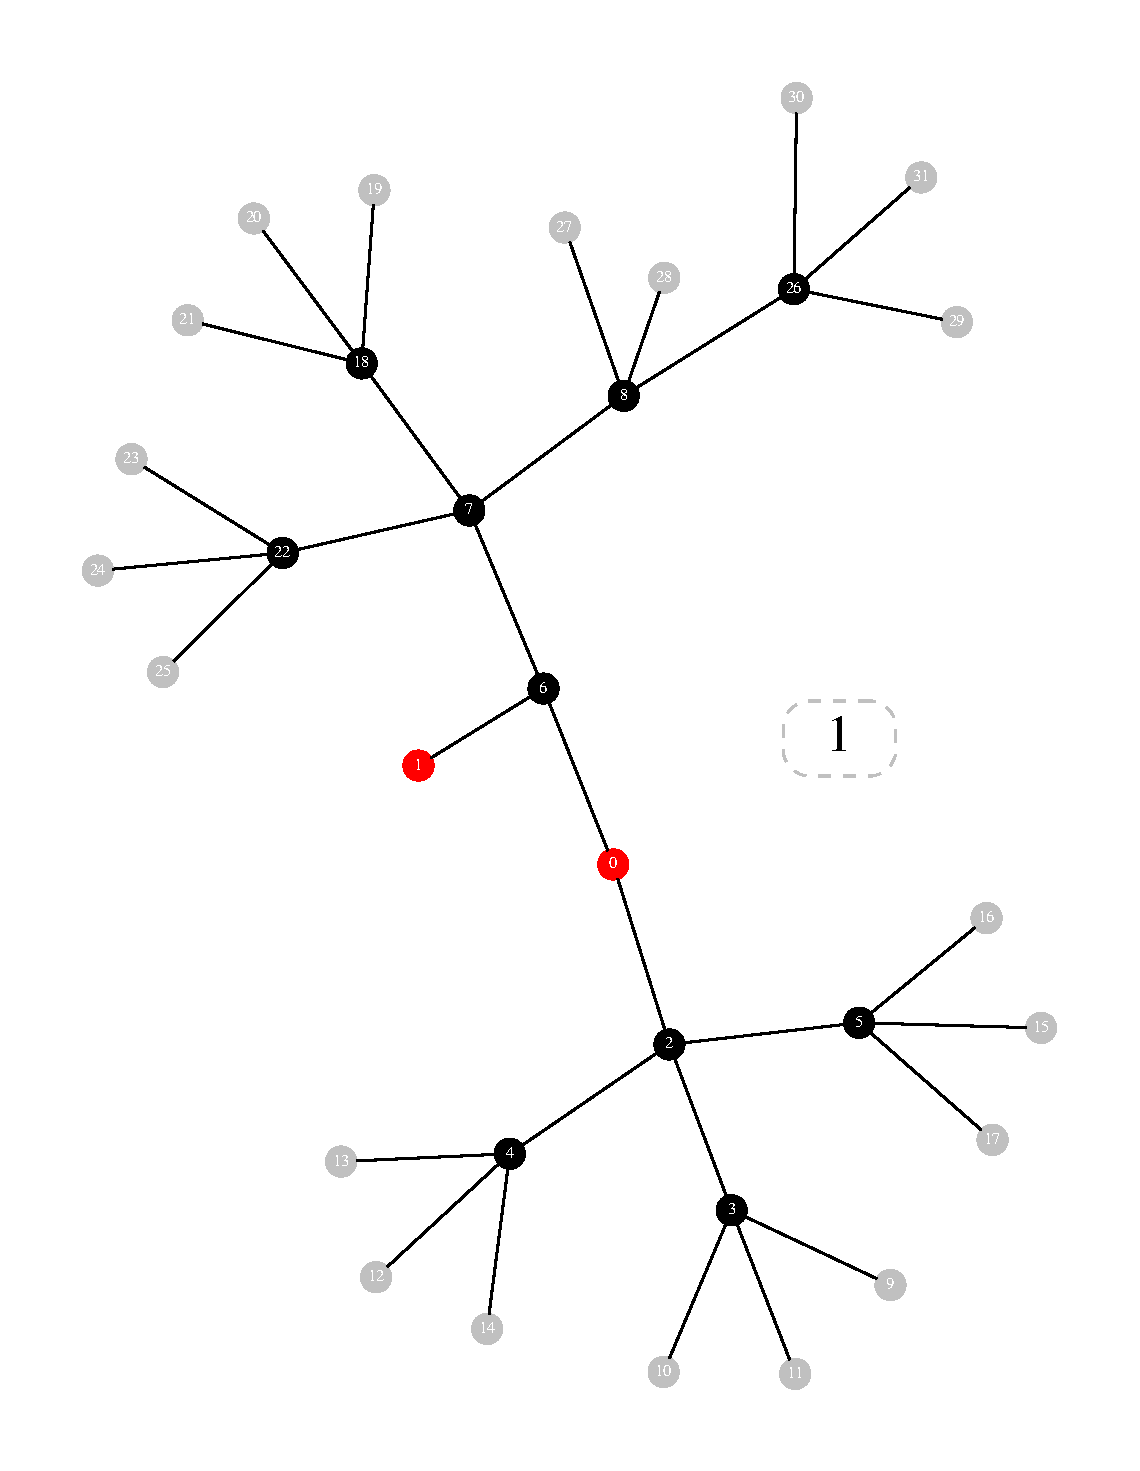
\includegraphics[scale=0.15]{mol_pictures/73.pdf}}
+
88
\raisebox{-.5\height}{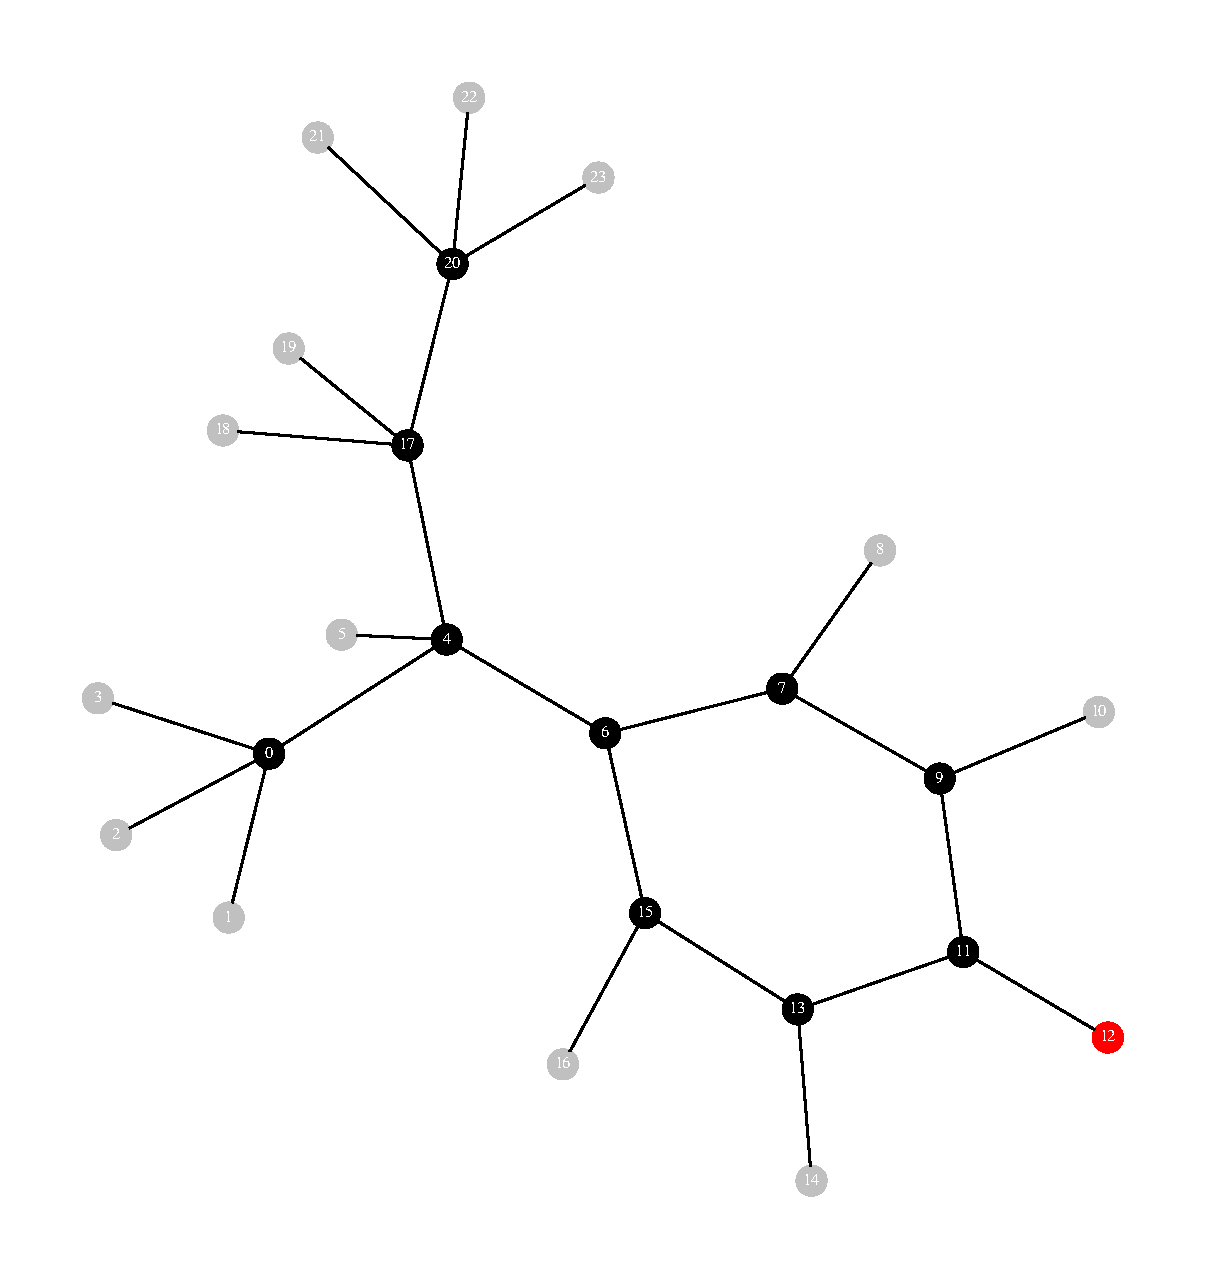
\includegraphics[scale=0.15]{mol_pictures/88.pdf}}
$$


reactant bonds broken:\begin{verbatim}
[(1, 12), (1, 13)]
\end{verbatim}
product bonds broken:\begin{verbatim}
[(0, 3), (0, 10)]
\end{verbatim}




\vspace{1cm}
\begin{verbatim}
more than one reactant
fragment matching found
free_energy dG is above threshold=0.0
Terminal.KEEP
\end{verbatim}
$$
48
\raisebox{-.5\height}{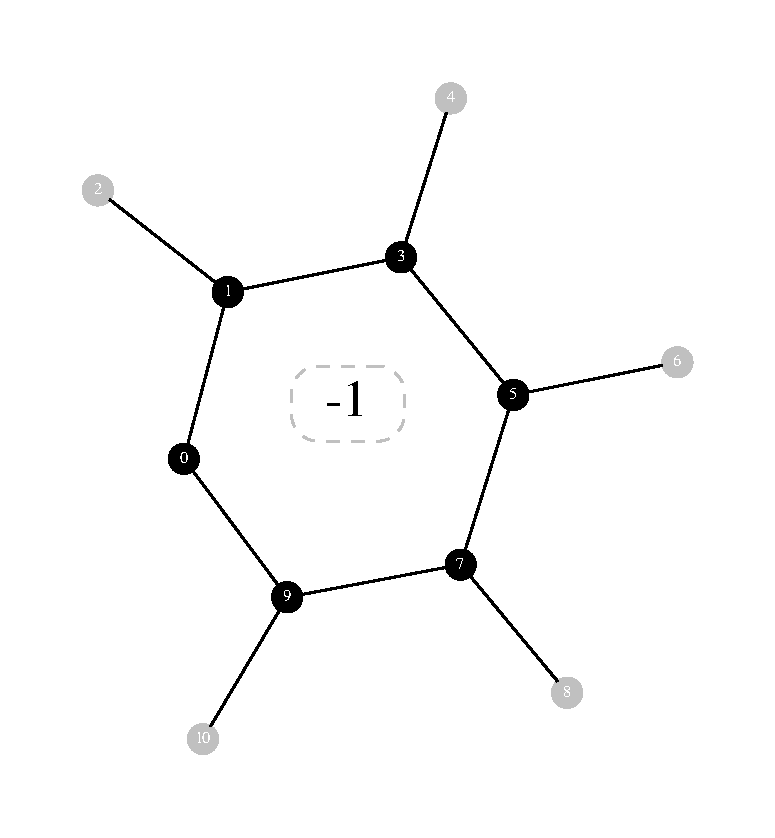
\includegraphics[scale=0.15]{mol_pictures/48.pdf}}
+
82
\raisebox{-.5\height}{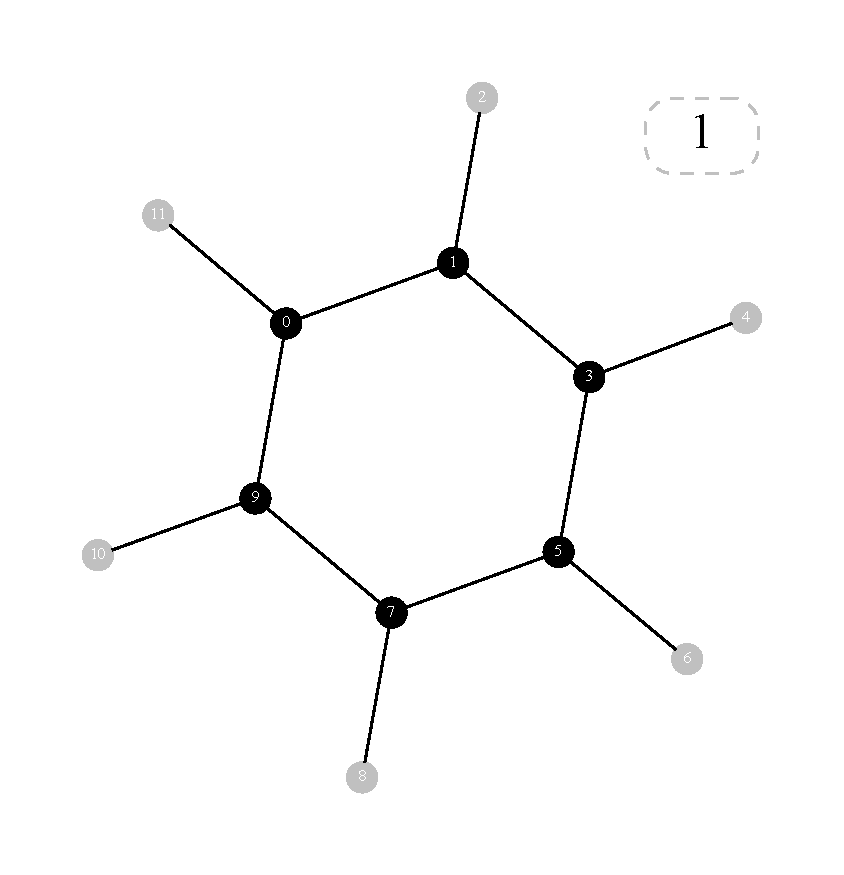
\includegraphics[scale=0.15]{mol_pictures/82.pdf}}
\xrightarrow[0.14]{1.41}
50
\raisebox{-.5\height}{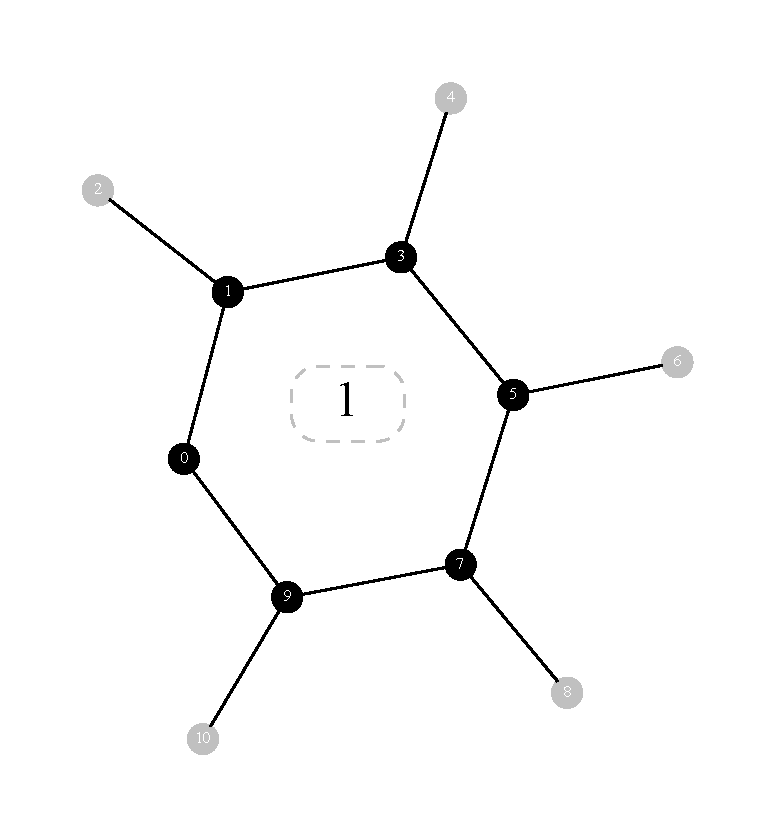
\includegraphics[scale=0.15]{mol_pictures/50.pdf}}
+
80
\raisebox{-.5\height}{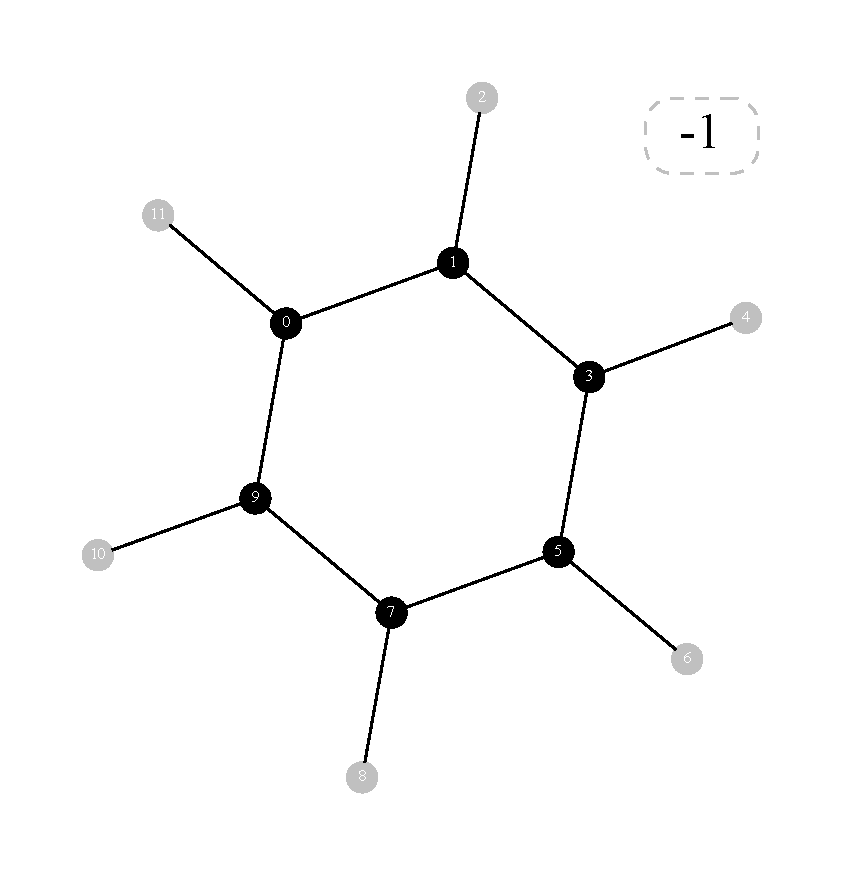
\includegraphics[scale=0.15]{mol_pictures/80.pdf}}
$$


reactant bonds broken:\begin{verbatim}
[(1, 0), (1, 11)]
\end{verbatim}
product bonds broken:\begin{verbatim}
[(1, 0), (1, 11)]
\end{verbatim}




\vspace{1cm}
\begin{verbatim}
more than one reactant
fragment matching found
free_energy dG is above threshold=0.0
Terminal.KEEP
\end{verbatim}
$$
48
\raisebox{-.5\height}{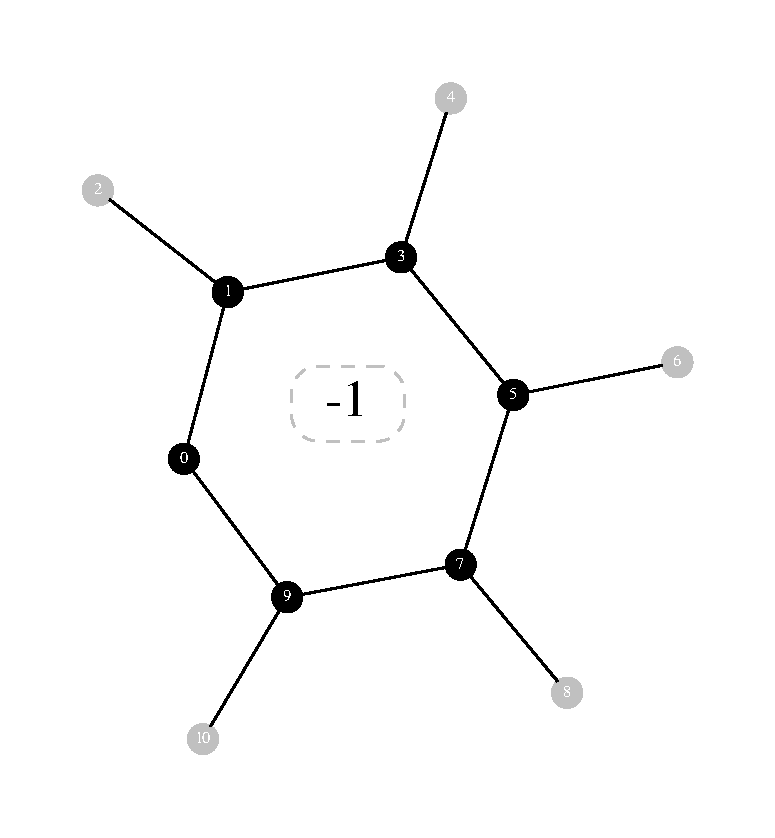
\includegraphics[scale=0.15]{mol_pictures/48.pdf}}
+
69
\raisebox{-.5\height}{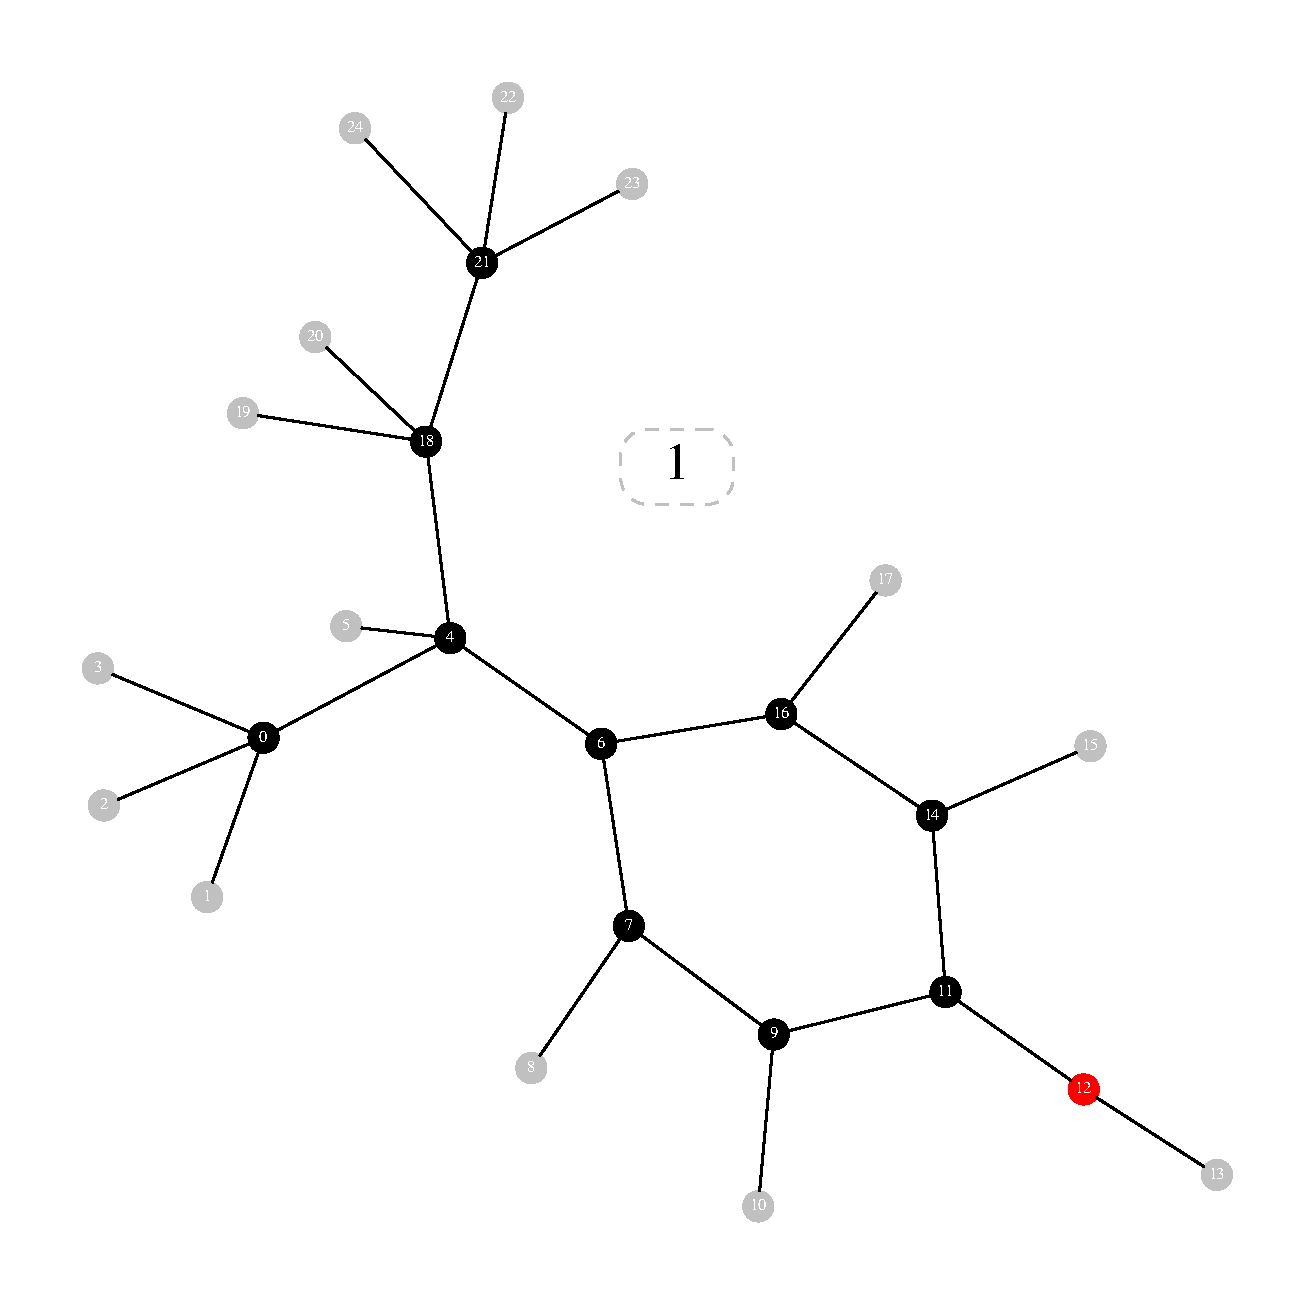
\includegraphics[scale=0.15]{mol_pictures/69.pdf}}
\xrightarrow[0.12]{1.22}
80
\raisebox{-.5\height}{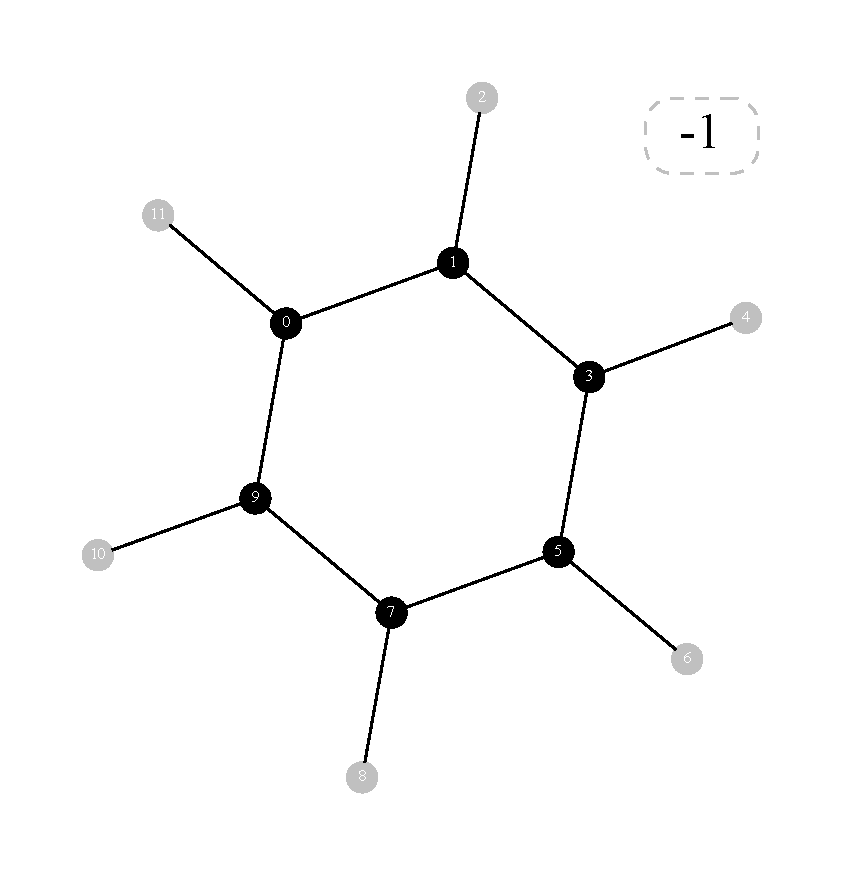
\includegraphics[scale=0.15]{mol_pictures/80.pdf}}
+
89
\raisebox{-.5\height}{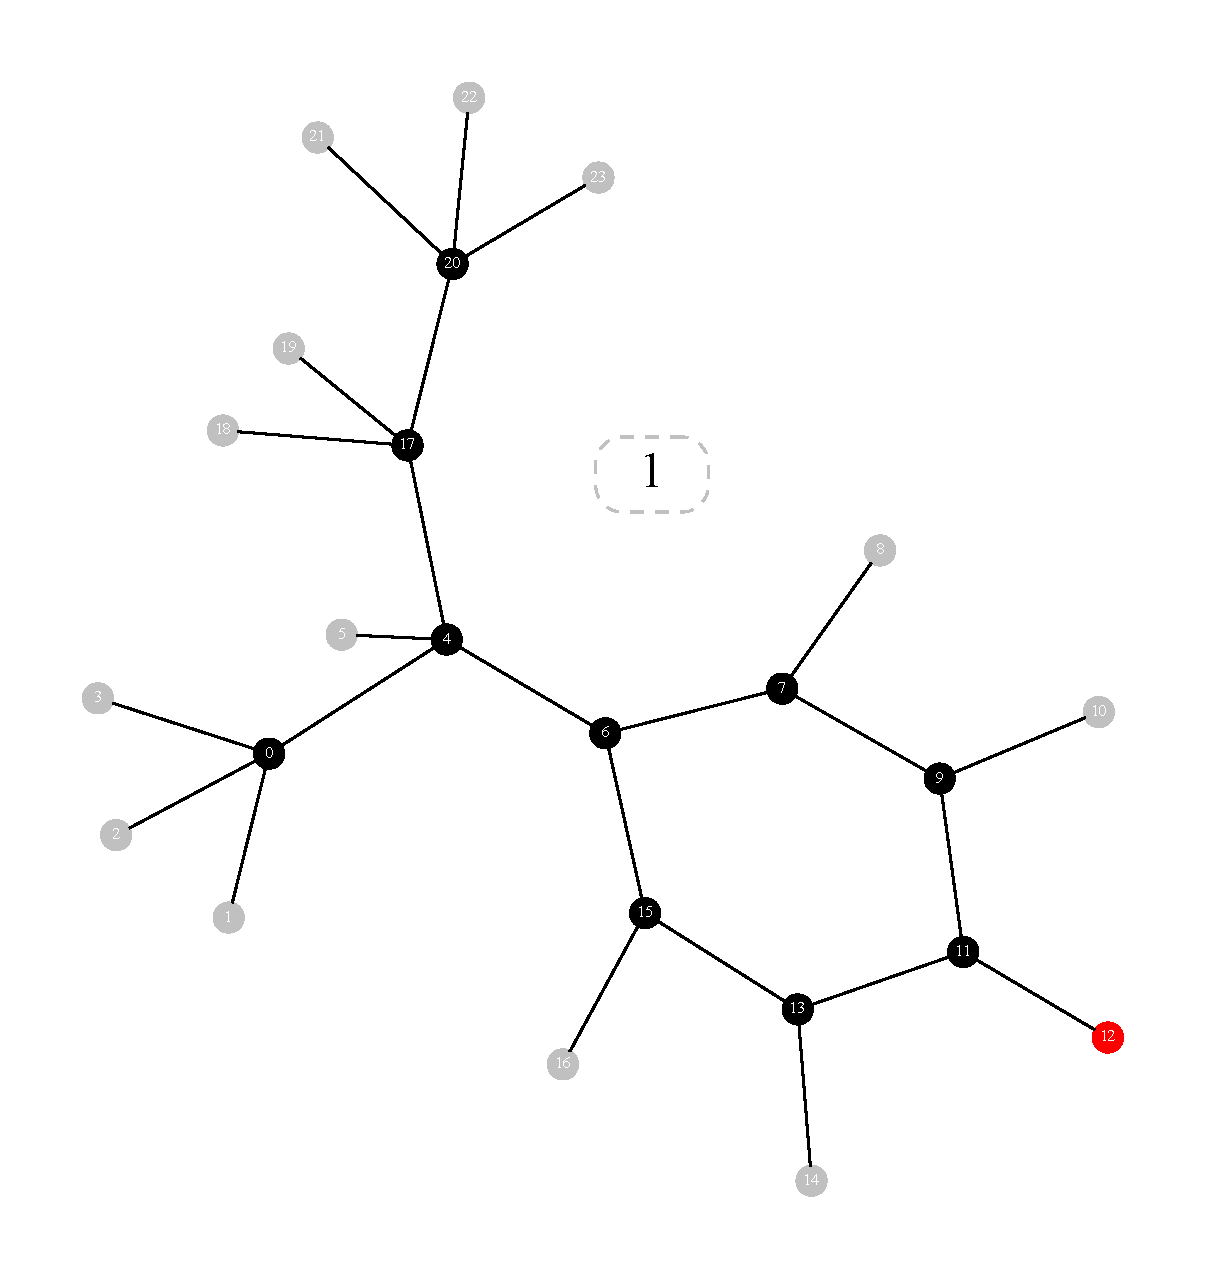
\includegraphics[scale=0.15]{mol_pictures/89.pdf}}
$$


reactant bonds broken:\begin{verbatim}
[(1, 12), (1, 13)]
\end{verbatim}
product bonds broken:\begin{verbatim}
[(0, 0), (0, 11)]
\end{verbatim}




\vspace{1cm}
\begin{verbatim}
more than one reactant
fragment matching found
free_energy dG is above threshold=0.0
Terminal.KEEP
\end{verbatim}
$$
54
\raisebox{-.5\height}{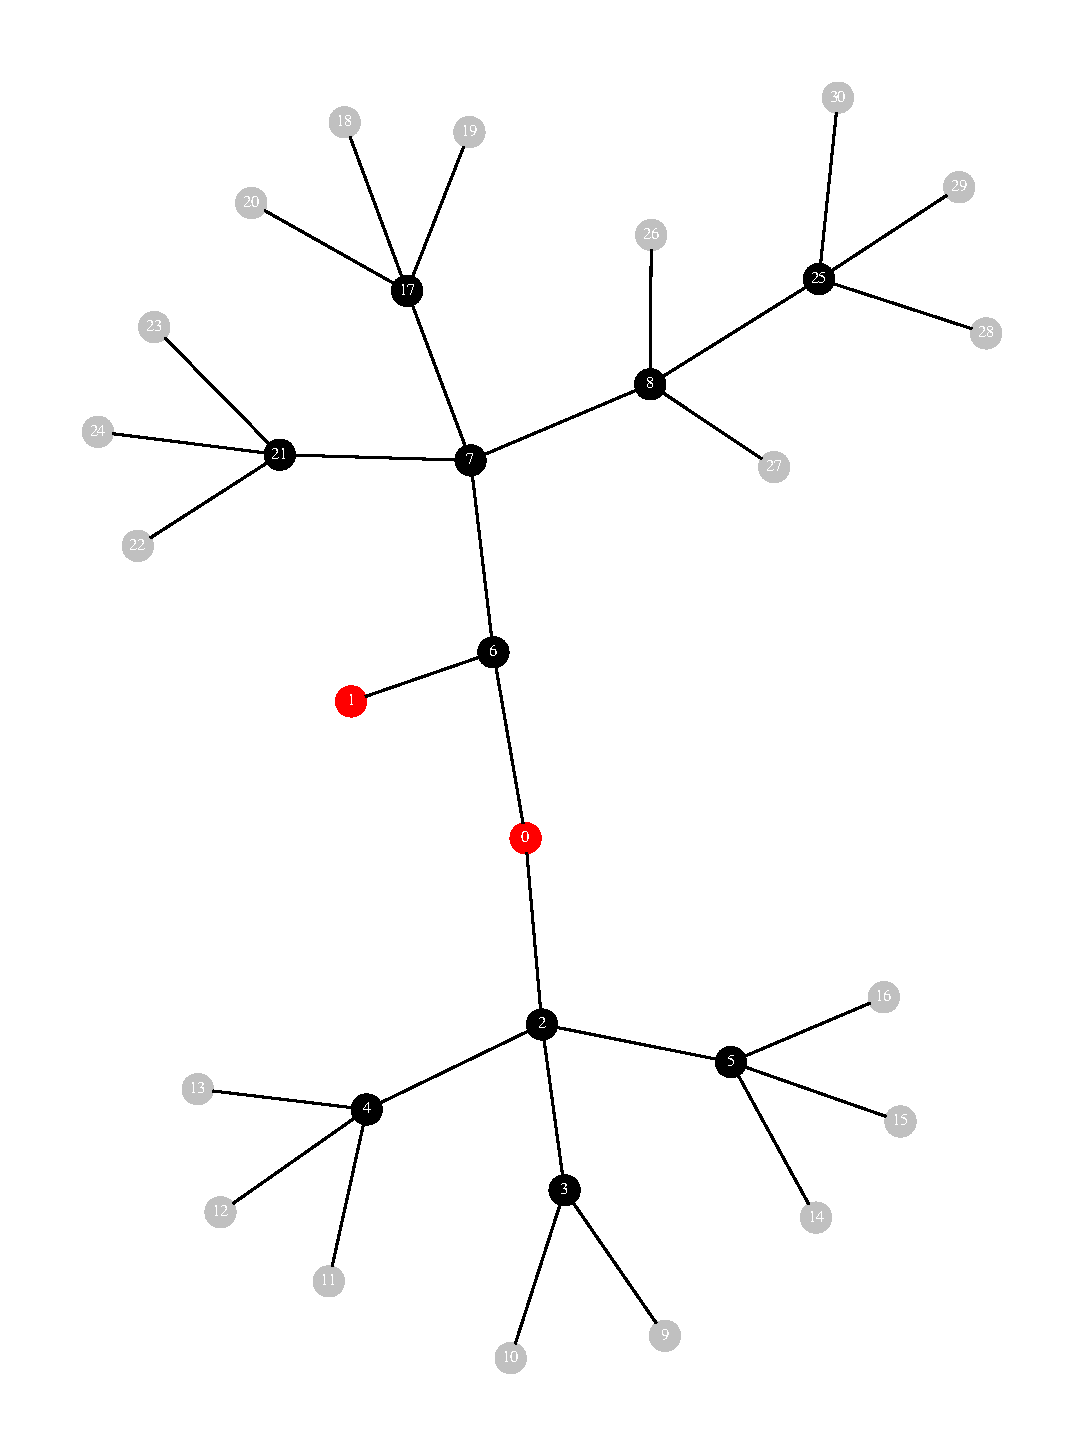
\includegraphics[scale=0.15]{mol_pictures/54.pdf}}
+
82
\raisebox{-.5\height}{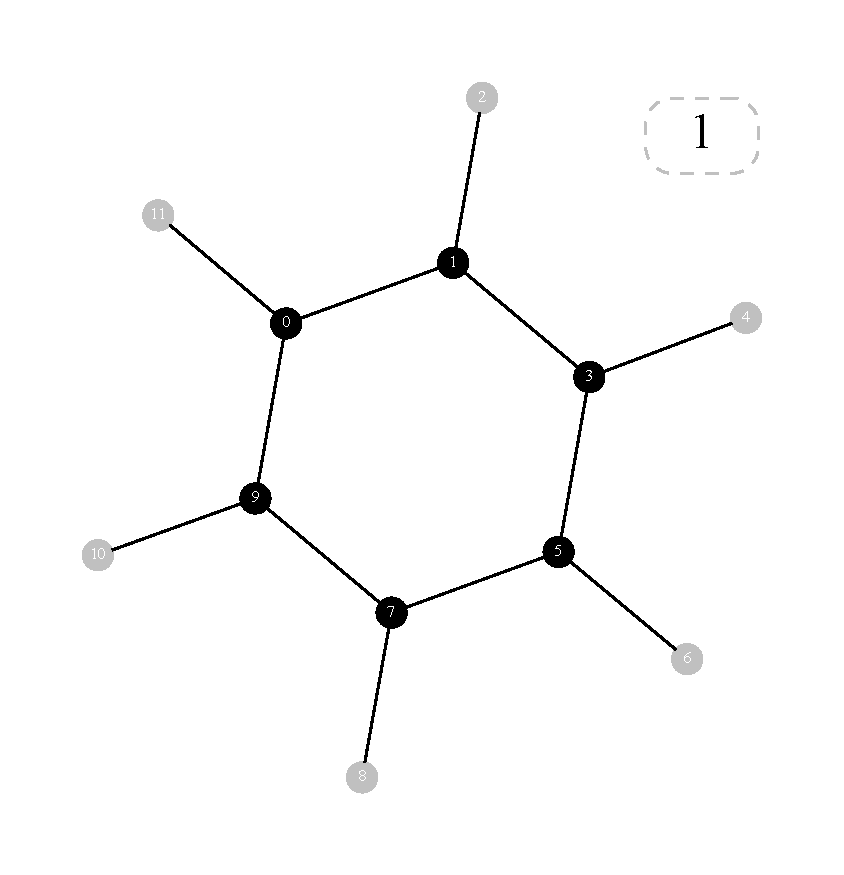
\includegraphics[scale=0.15]{mol_pictures/82.pdf}}
\xrightarrow[0.09]{0.89}
49
\raisebox{-.5\height}{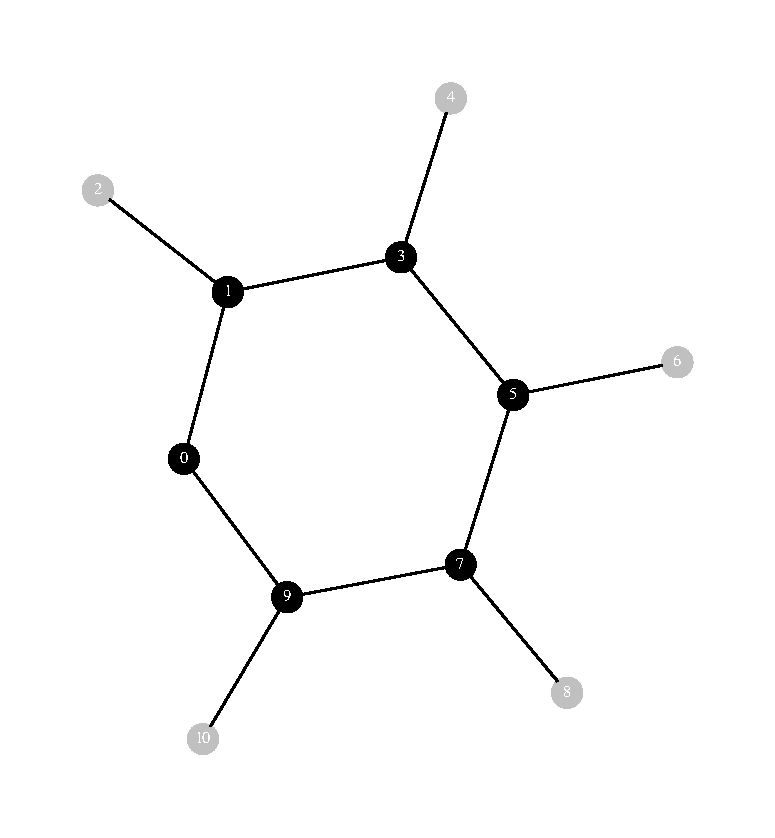
\includegraphics[scale=0.15]{mol_pictures/49.pdf}}
+
73
\raisebox{-.5\height}{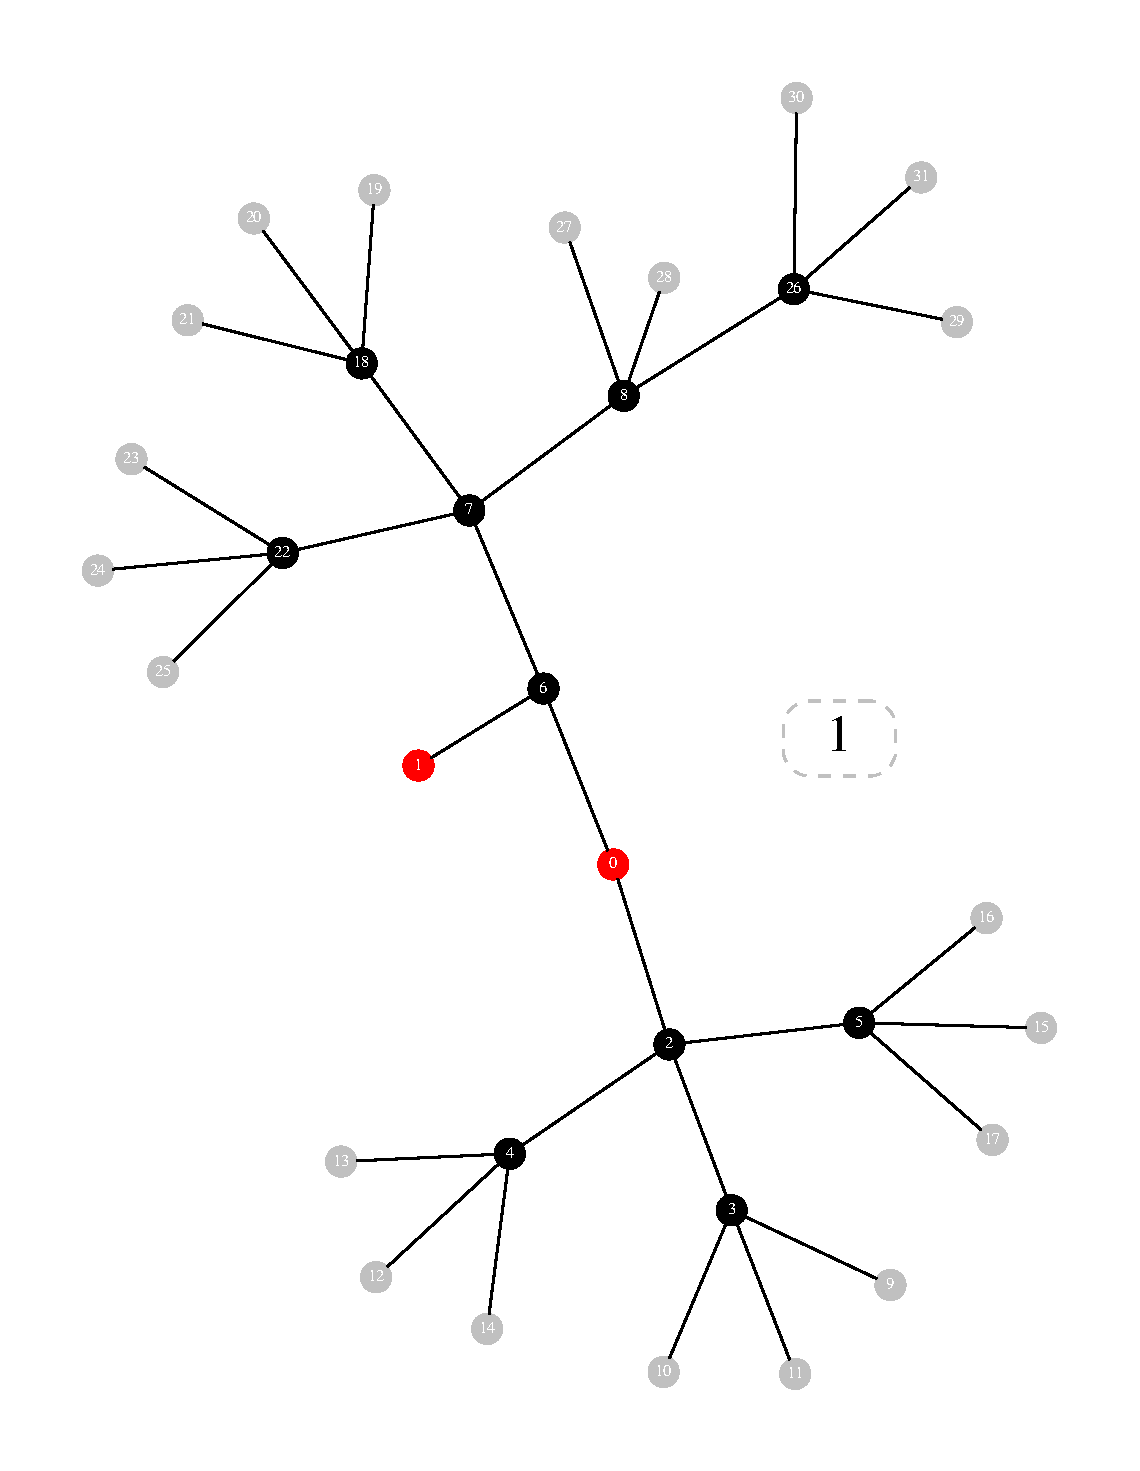
\includegraphics[scale=0.15]{mol_pictures/73.pdf}}
$$


reactant bonds broken:\begin{verbatim}
[(1, 0), (1, 11)]
\end{verbatim}
product bonds broken:\begin{verbatim}
[(1, 3), (1, 10)]
\end{verbatim}




\vspace{1cm}
\begin{verbatim}
more than one reactant
fragment matching found
free_energy dG is above threshold=0.0
Terminal.KEEP
\end{verbatim}
$$
48
\raisebox{-.5\height}{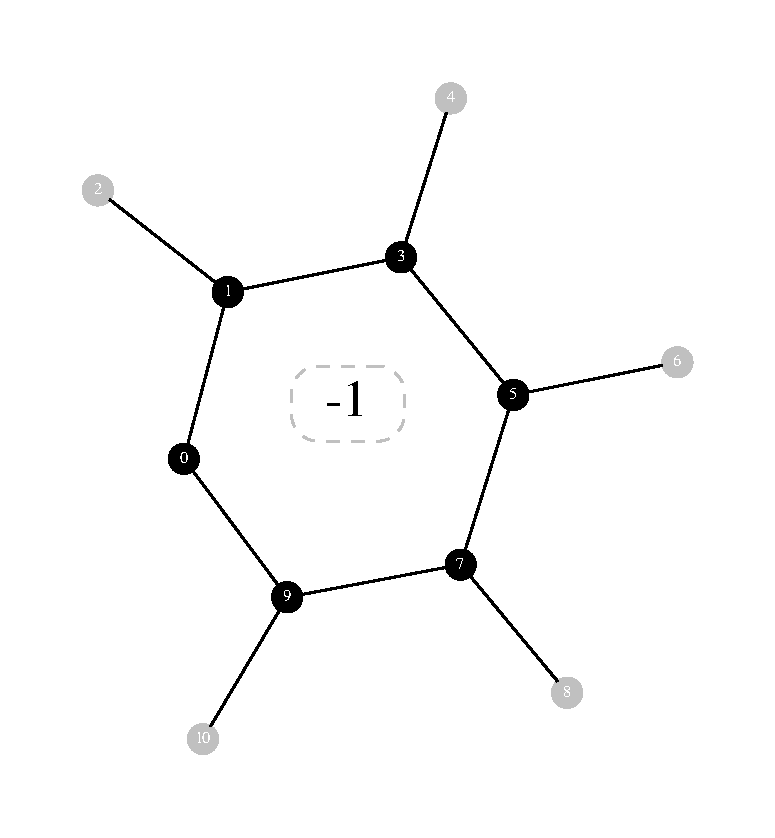
\includegraphics[scale=0.15]{mol_pictures/48.pdf}}
+
70
\raisebox{-.5\height}{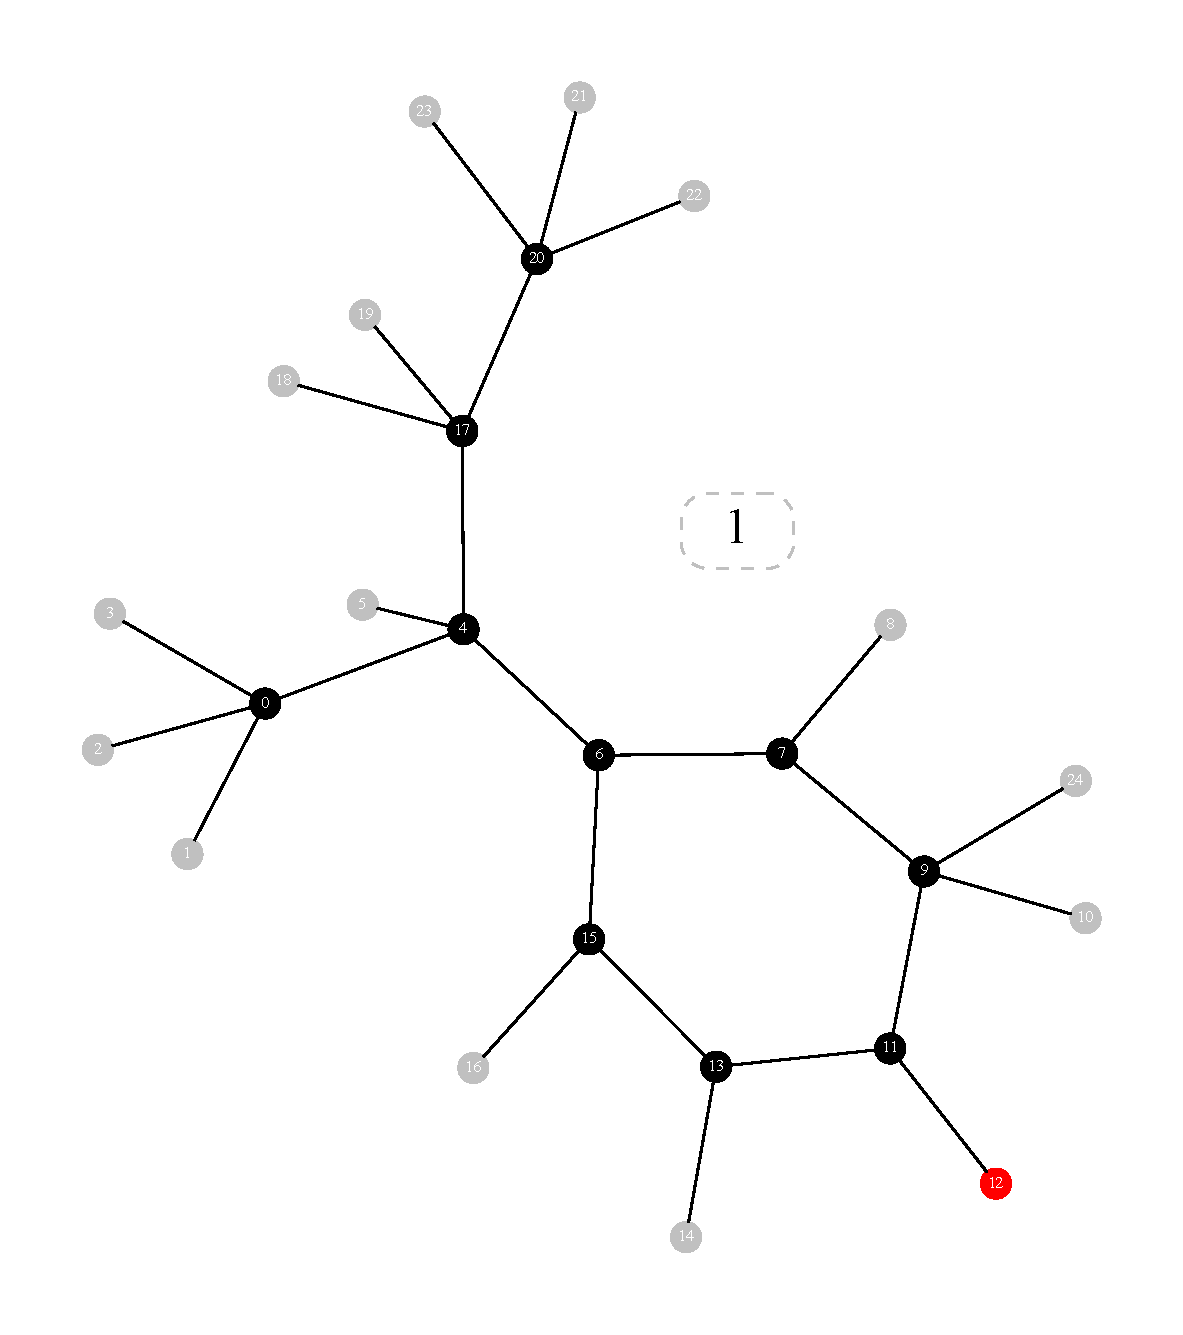
\includegraphics[scale=0.15]{mol_pictures/70.pdf}}
\xrightarrow[0.01]{0.05}
80
\raisebox{-.5\height}{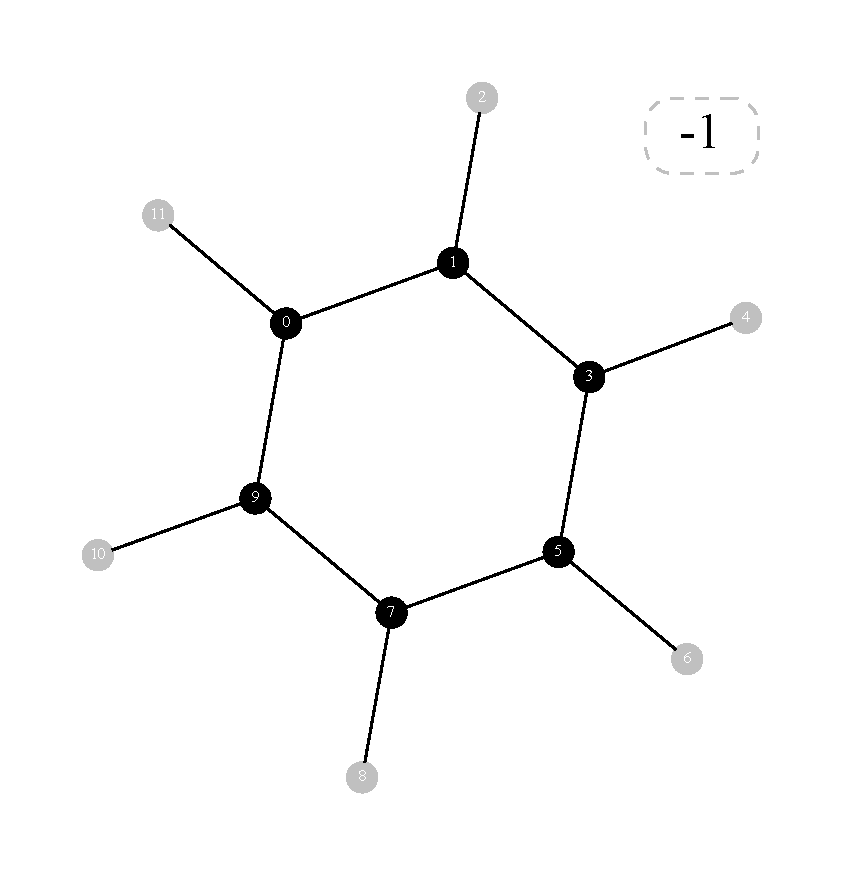
\includegraphics[scale=0.15]{mol_pictures/80.pdf}}
+
89
\raisebox{-.5\height}{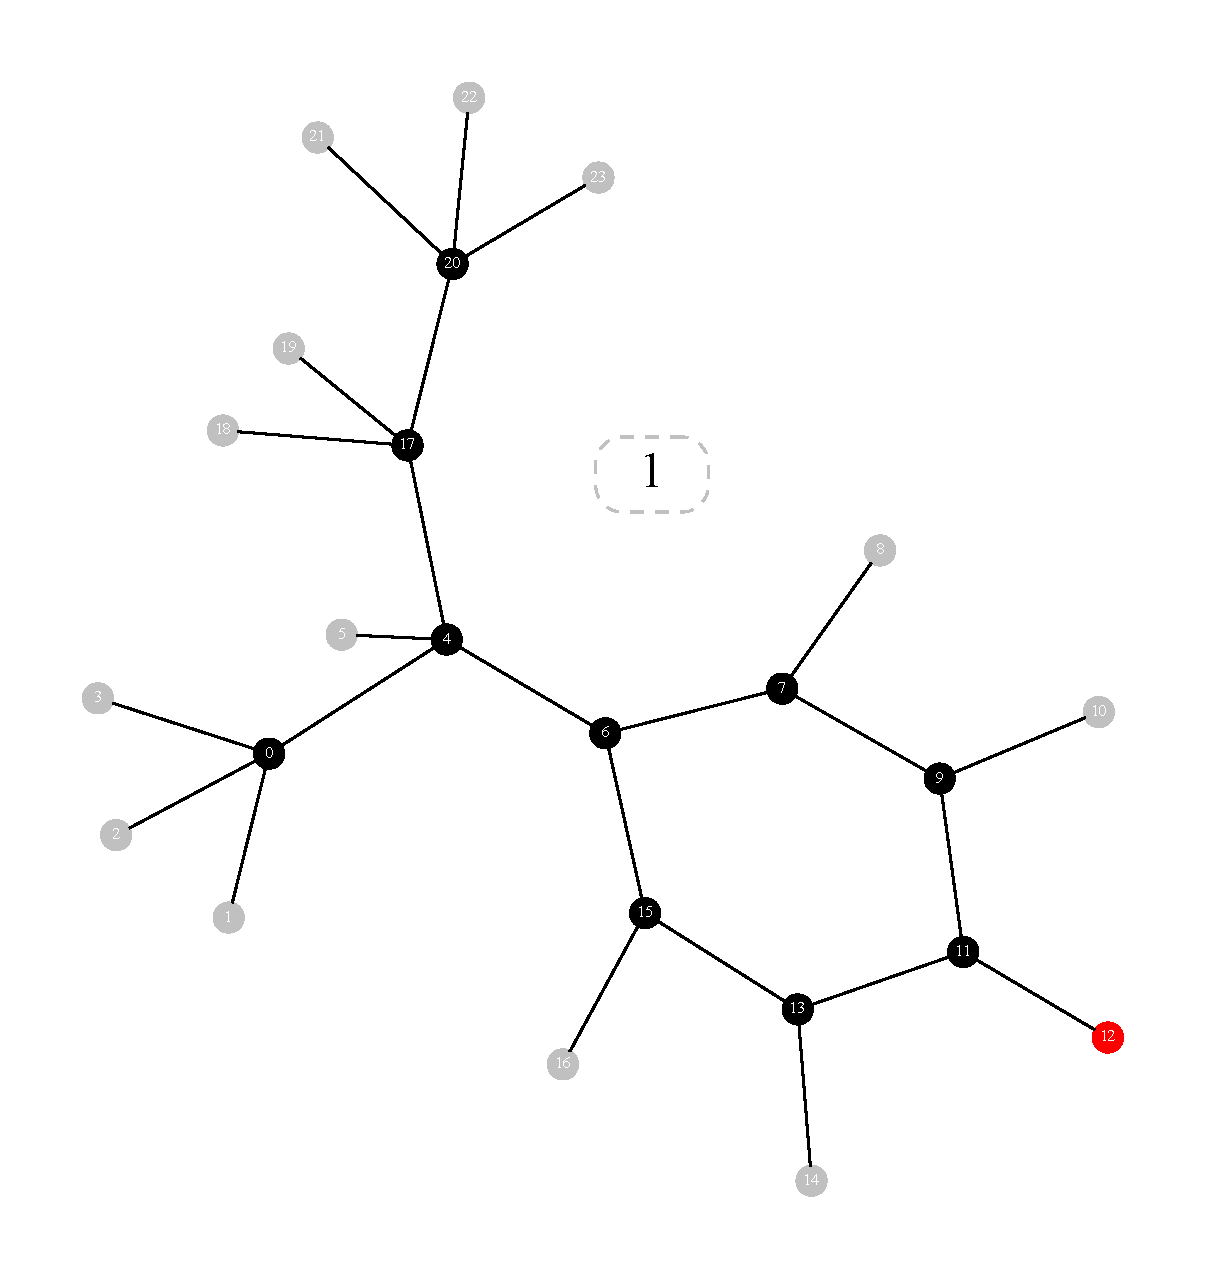
\includegraphics[scale=0.15]{mol_pictures/89.pdf}}
$$


reactant bonds broken:\begin{verbatim}
[(1, 9), (1, 10)]
\end{verbatim}
product bonds broken:\begin{verbatim}
[(0, 0), (0, 11)]
\end{verbatim}




\vspace{1cm}
\begin{verbatim}
more than one reactant
fragment matching found
free_energy dG is above threshold=0.0
Terminal.KEEP
\end{verbatim}
$$
80
\raisebox{-.5\height}{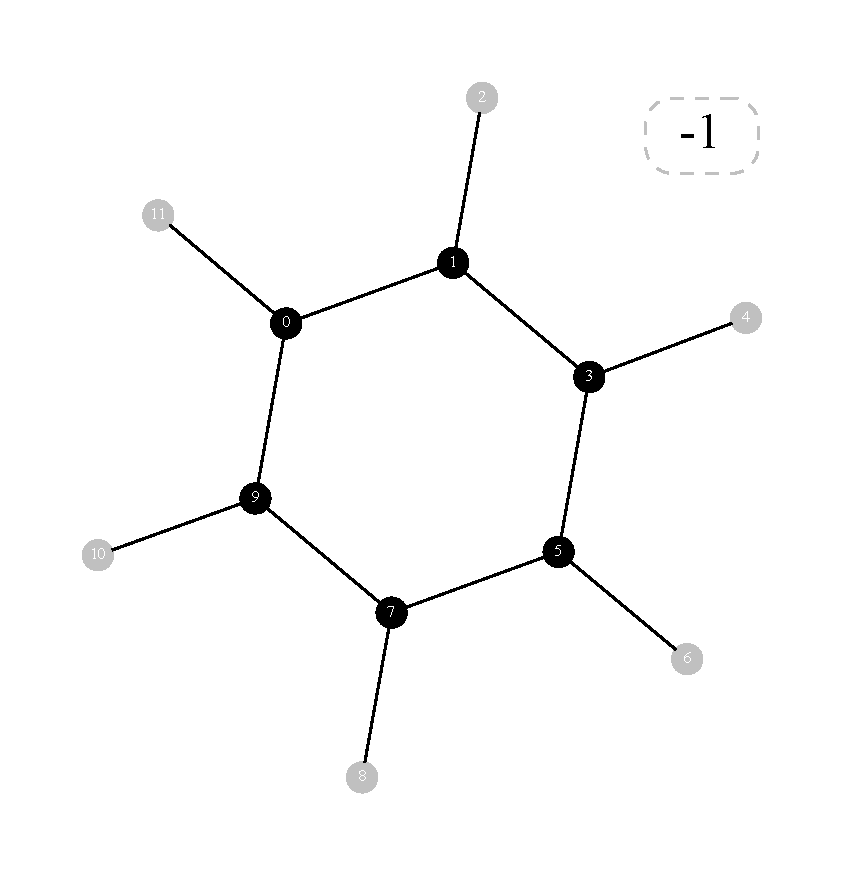
\includegraphics[scale=0.15]{mol_pictures/80.pdf}}
+
89
\raisebox{-.5\height}{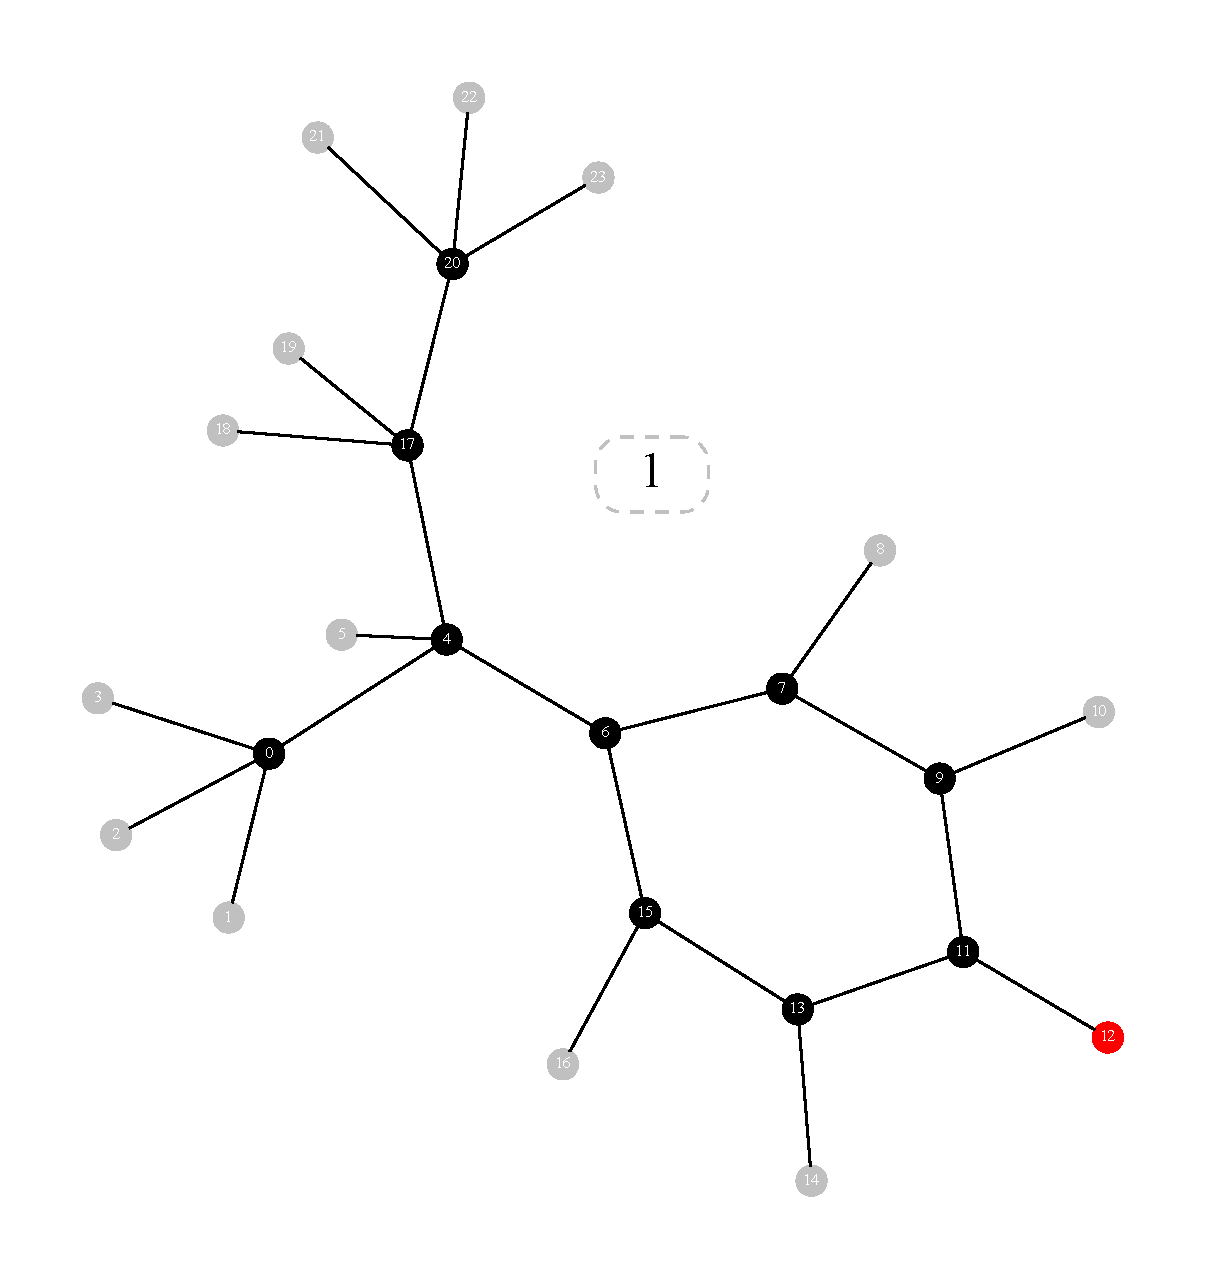
\includegraphics[scale=0.15]{mol_pictures/89.pdf}}
\xrightarrow[0.10]{1.03}
50
\raisebox{-.5\height}{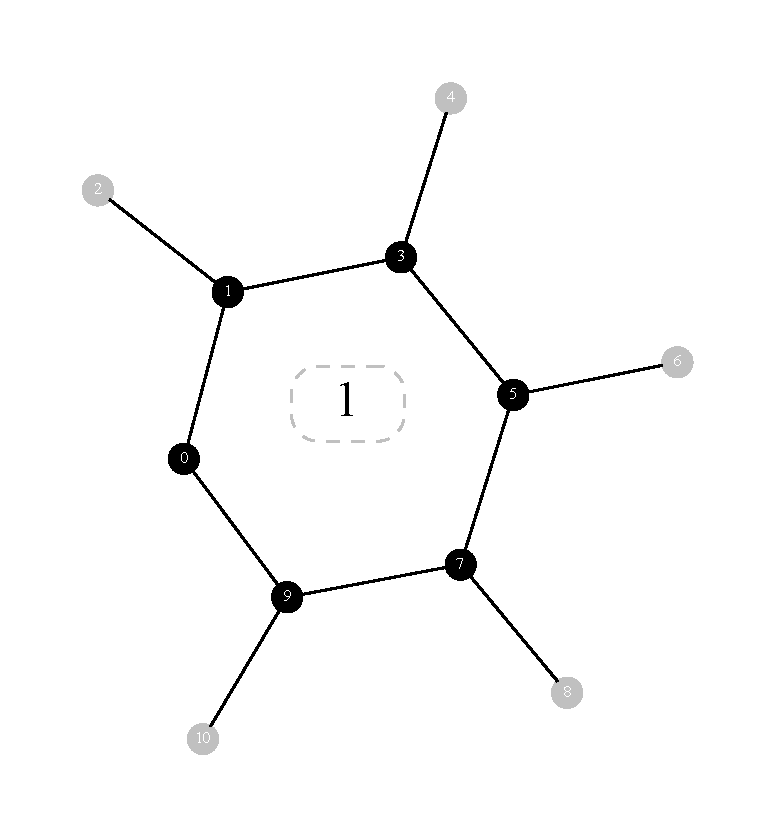
\includegraphics[scale=0.15]{mol_pictures/50.pdf}}
+
65
\raisebox{-.5\height}{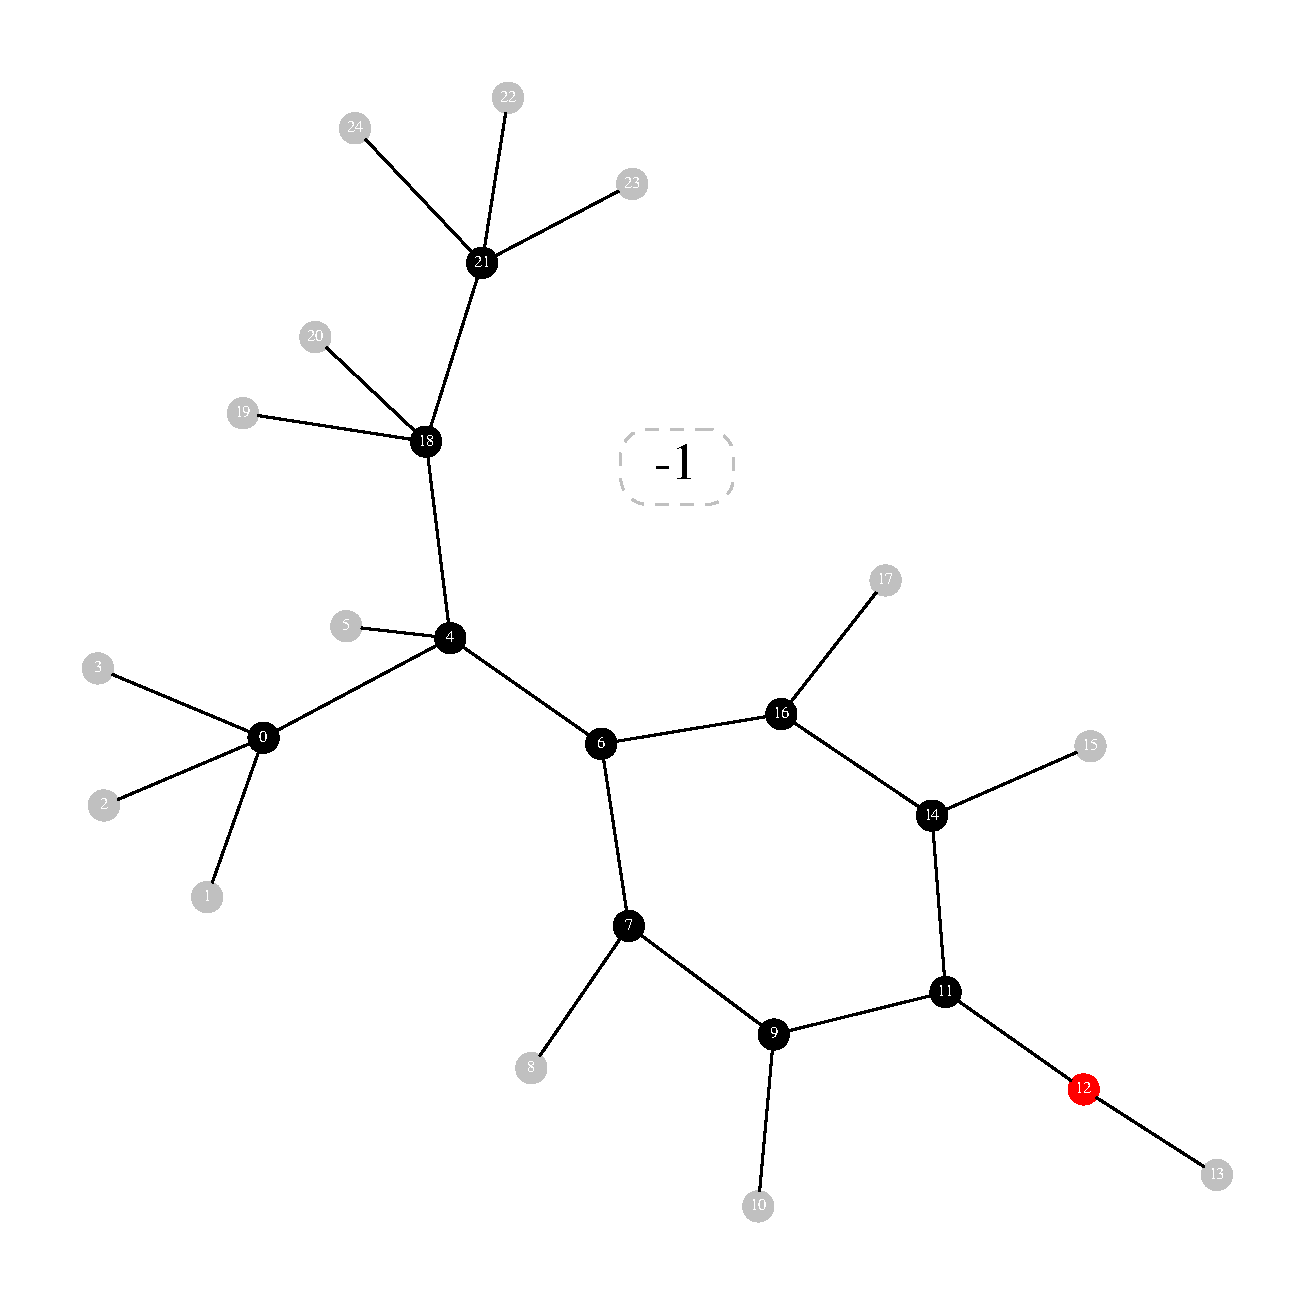
\includegraphics[scale=0.15]{mol_pictures/65.pdf}}
$$


reactant bonds broken:\begin{verbatim}
[(0, 0), (0, 11)]
\end{verbatim}
product bonds broken:\begin{verbatim}
[(1, 12), (1, 13)]
\end{verbatim}




\vspace{1cm}
\begin{verbatim}
more than one reactant
fragment matching found
free_energy dG is above threshold=0.0
Terminal.KEEP
\end{verbatim}
$$
80
\raisebox{-.5\height}{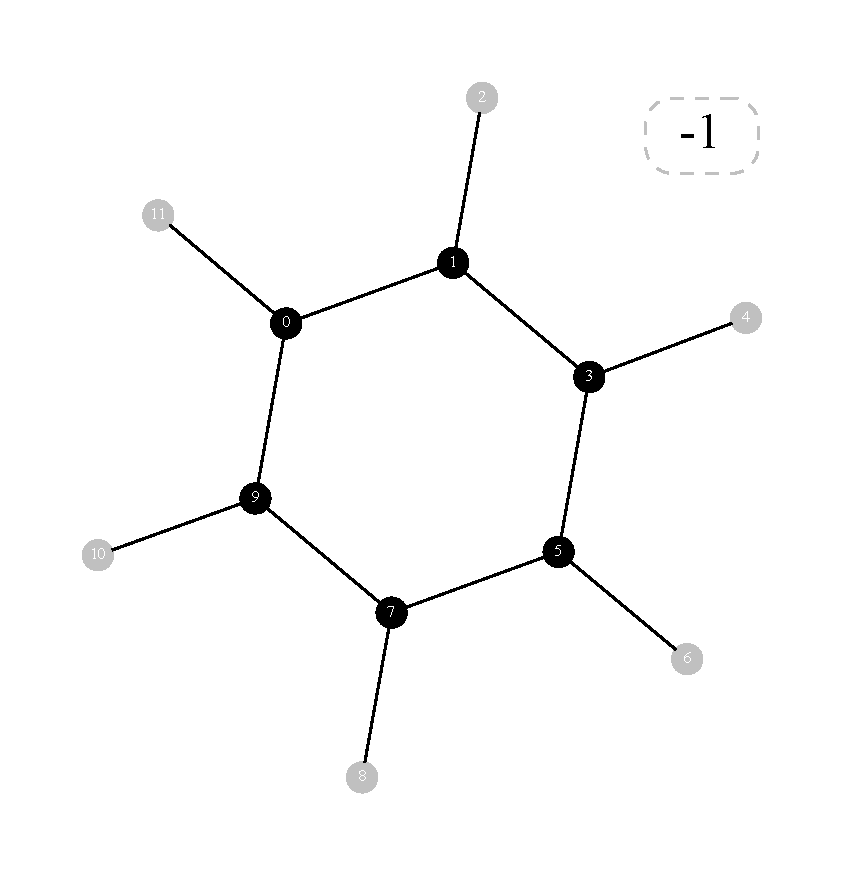
\includegraphics[scale=0.15]{mol_pictures/80.pdf}}
+
89
\raisebox{-.5\height}{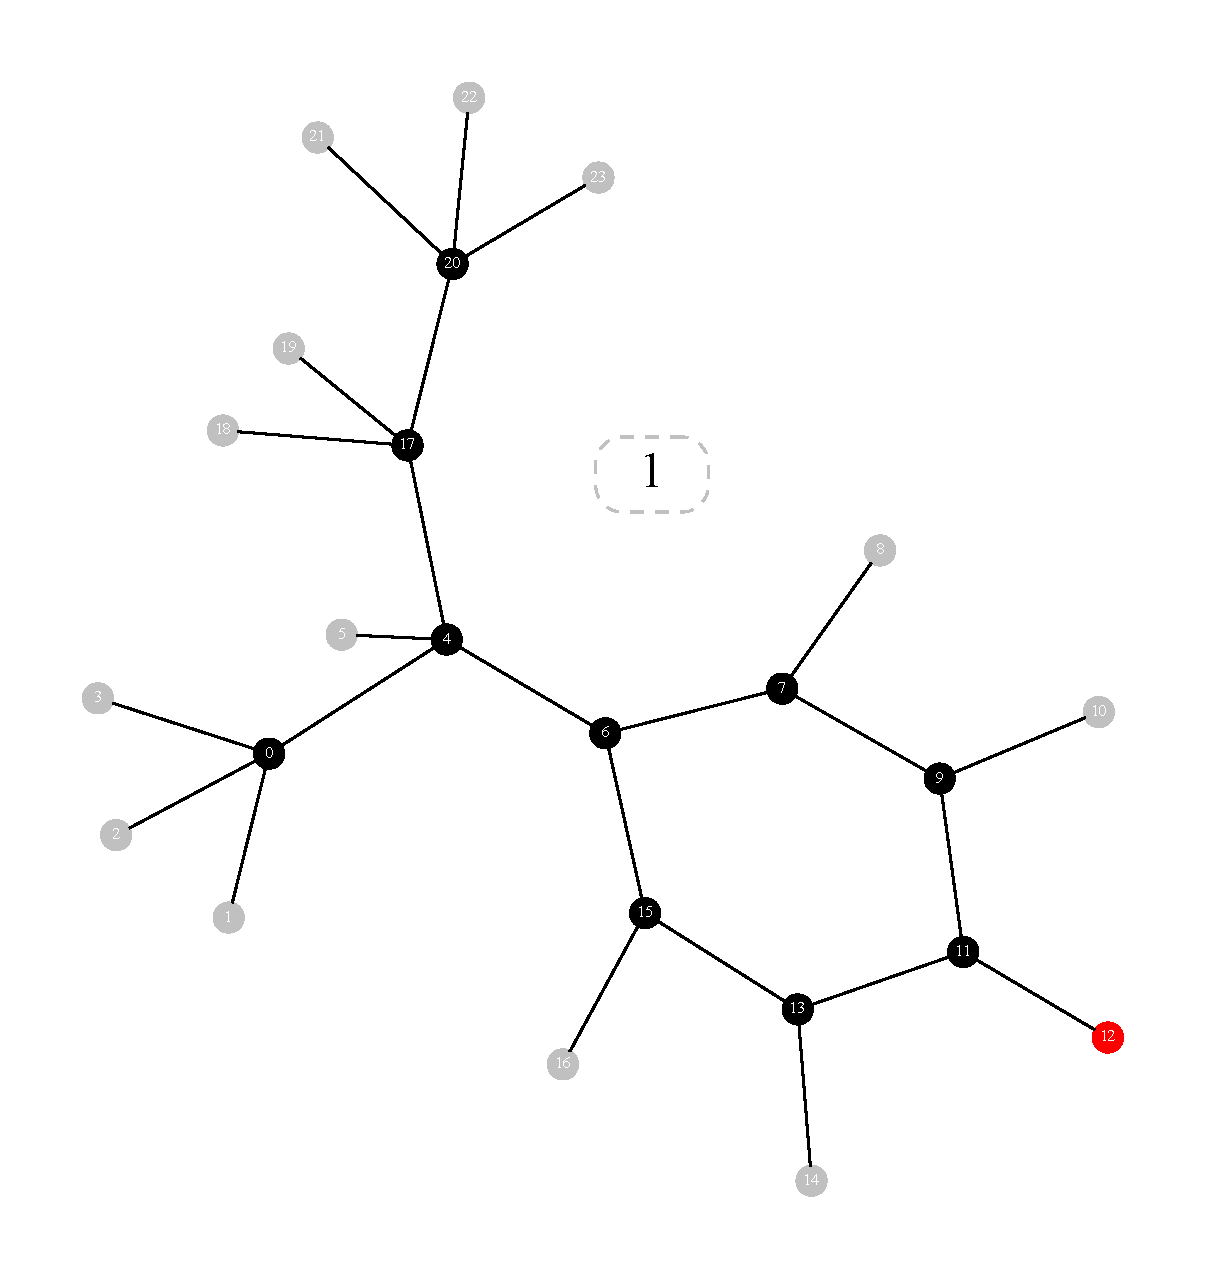
\includegraphics[scale=0.15]{mol_pictures/89.pdf}}
\xrightarrow[0.02]{0.18}
50
\raisebox{-.5\height}{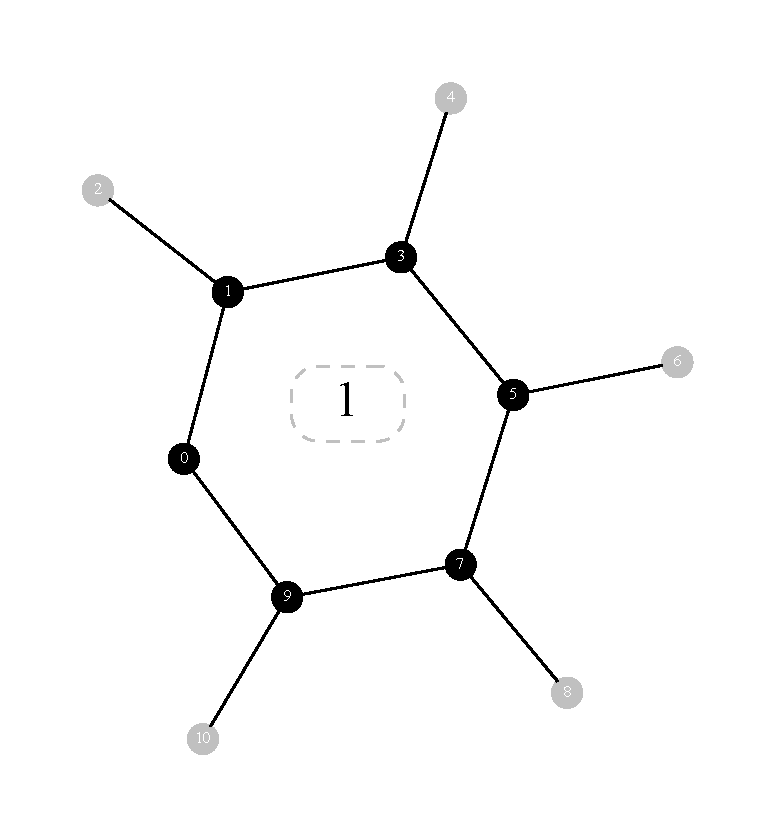
\includegraphics[scale=0.15]{mol_pictures/50.pdf}}
+
66
\raisebox{-.5\height}{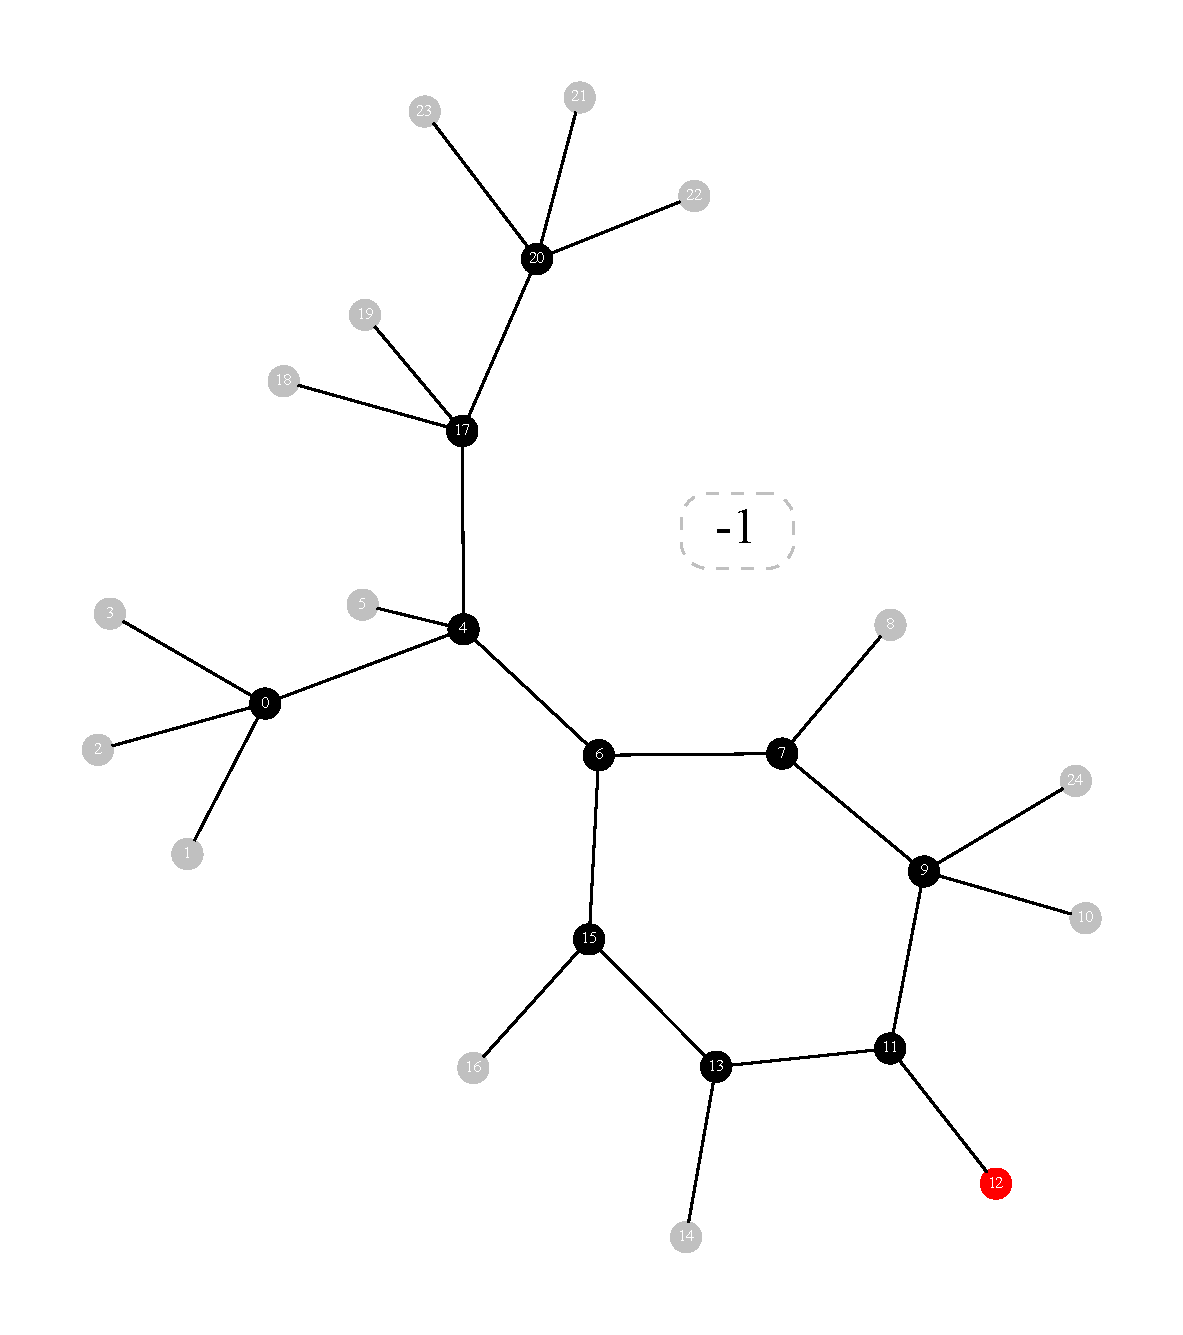
\includegraphics[scale=0.15]{mol_pictures/66.pdf}}
$$


reactant bonds broken:\begin{verbatim}
[(0, 0), (0, 11)]
\end{verbatim}
product bonds broken:\begin{verbatim}
[(1, 9), (1, 10)]
\end{verbatim}




\vspace{1cm}
\begin{verbatim}
more than one reactant
fragment matching found
free_energy dG is above threshold=0.0
Terminal.KEEP
\end{verbatim}
$$
81
\raisebox{-.5\height}{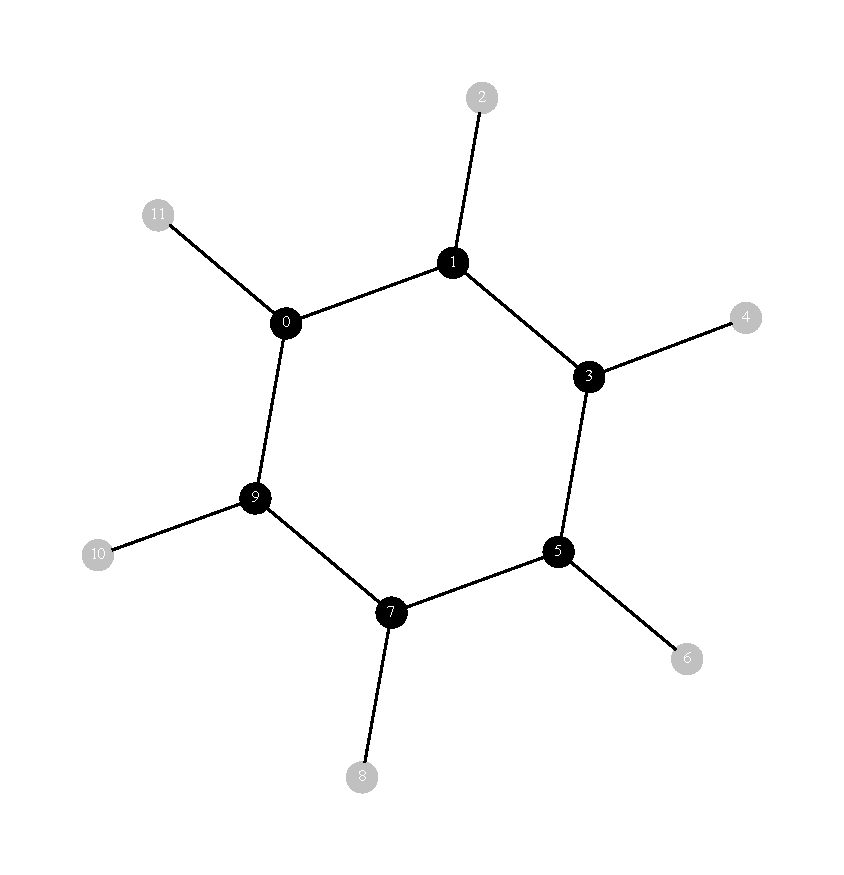
\includegraphics[scale=0.15]{mol_pictures/81.pdf}}
+
87
\raisebox{-.5\height}{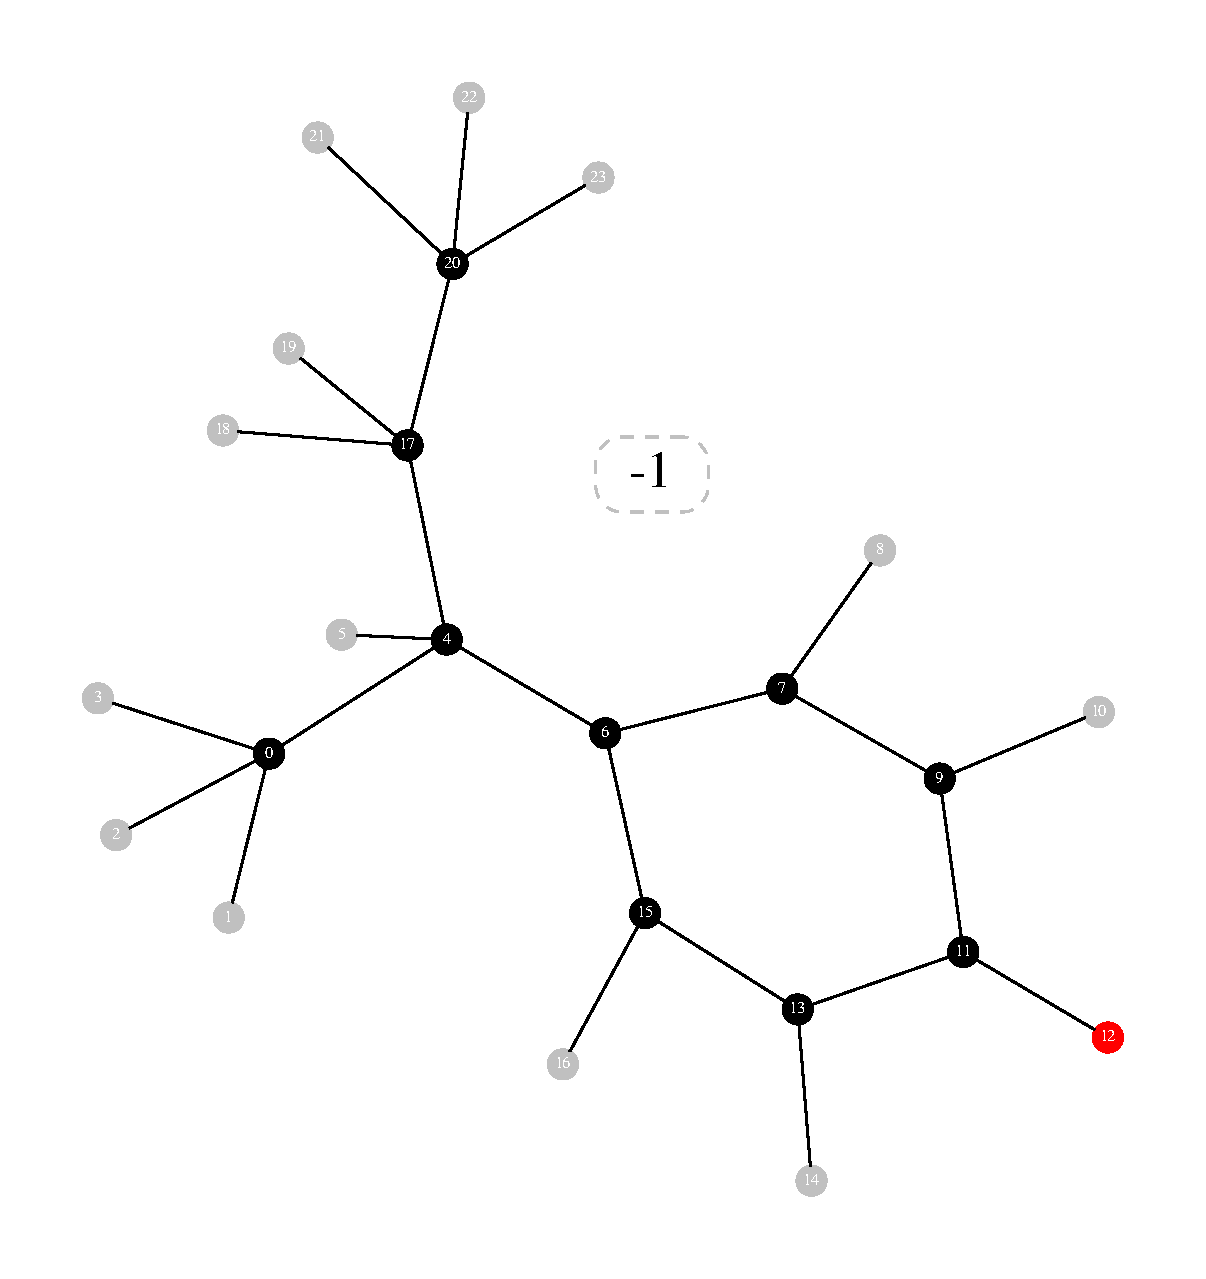
\includegraphics[scale=0.15]{mol_pictures/87.pdf}}
\xrightarrow[0.20]{2.01}
48
\raisebox{-.5\height}{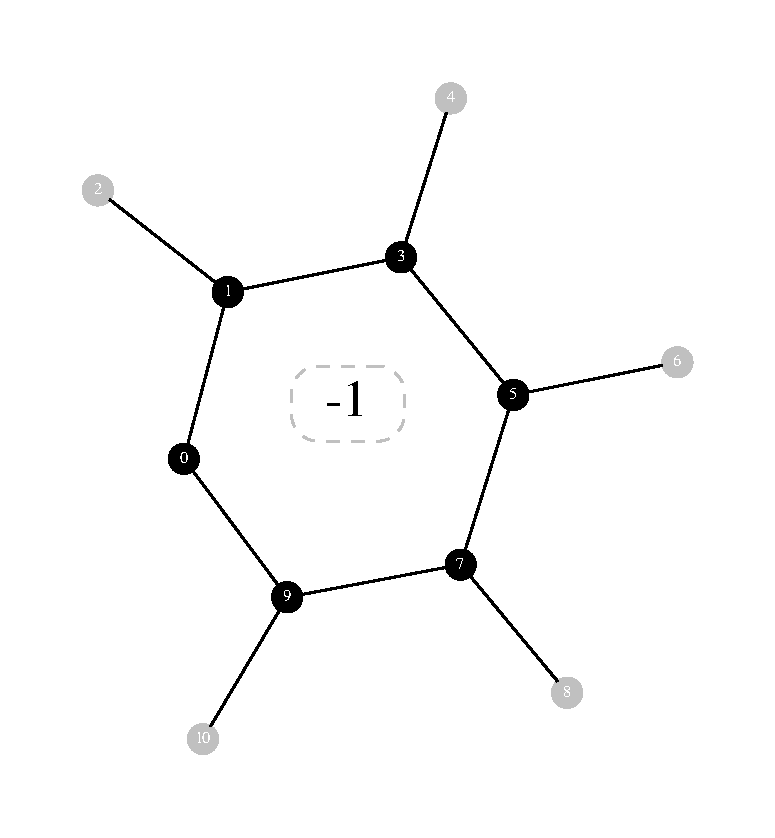
\includegraphics[scale=0.15]{mol_pictures/48.pdf}}
+
67
\raisebox{-.5\height}{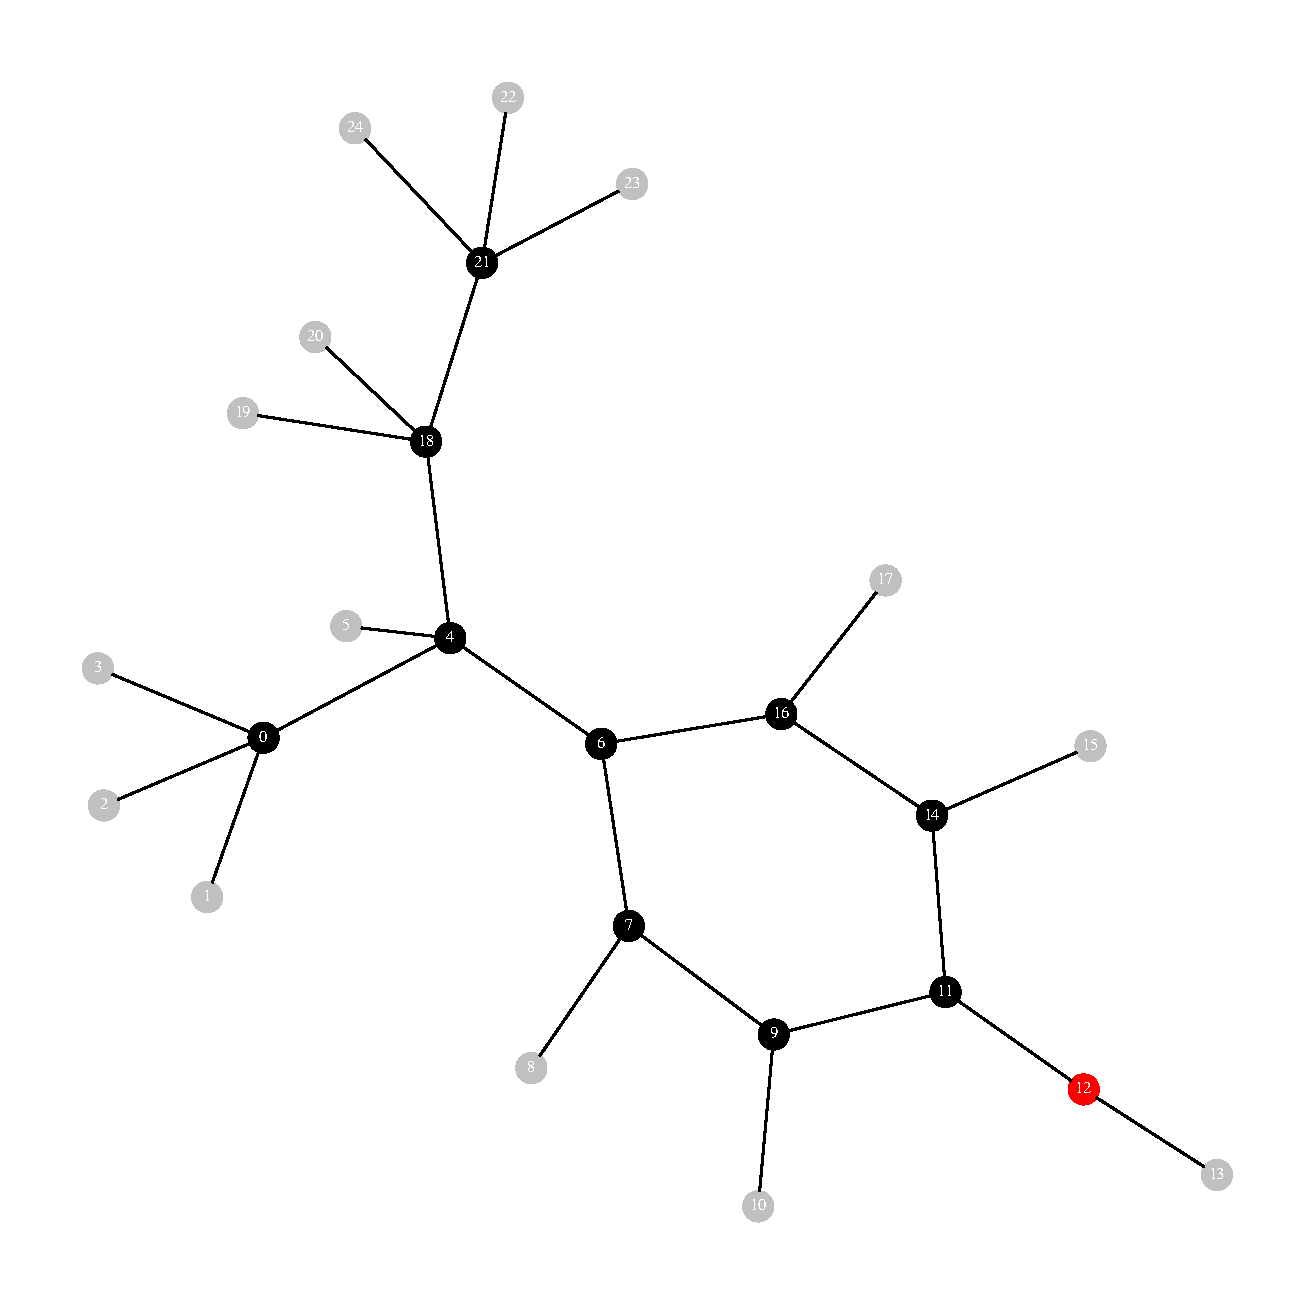
\includegraphics[scale=0.15]{mol_pictures/67.pdf}}
$$


reactant bonds broken:\begin{verbatim}
[(0, 0), (0, 11)]
\end{verbatim}
product bonds broken:\begin{verbatim}
[(1, 12), (1, 13)]
\end{verbatim}




\vspace{1cm}
\begin{verbatim}
more than one reactant
fragment matching found
free_energy dG is above threshold=0.0
Terminal.KEEP
\end{verbatim}
$$
81
\raisebox{-.5\height}{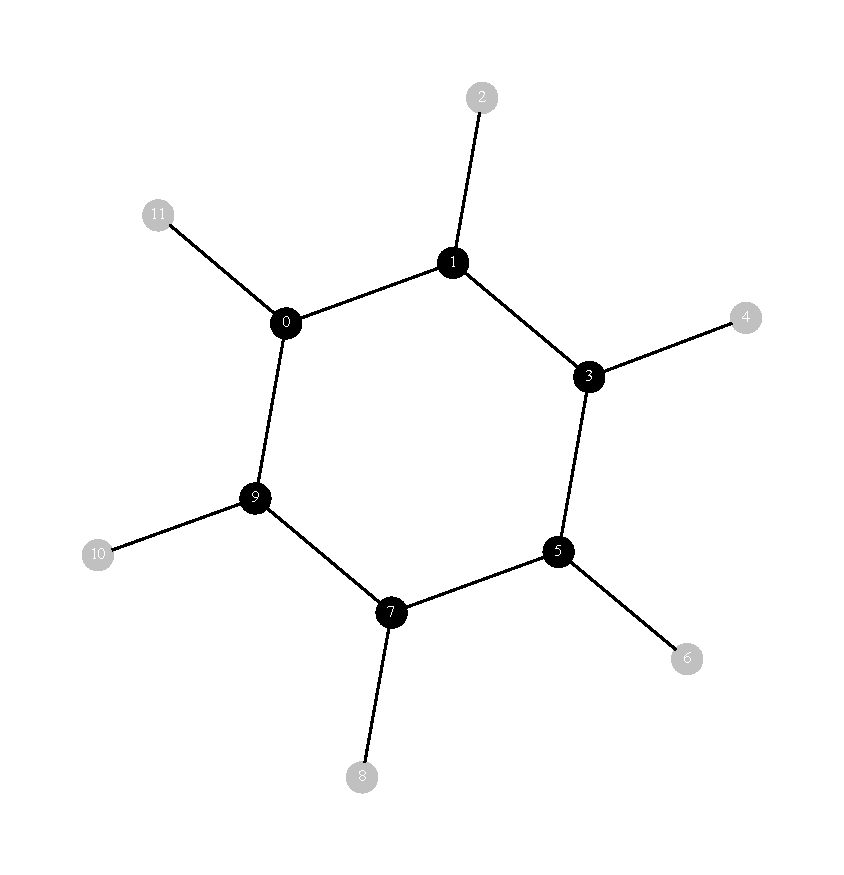
\includegraphics[scale=0.15]{mol_pictures/81.pdf}}
+
83
\raisebox{-.5\height}{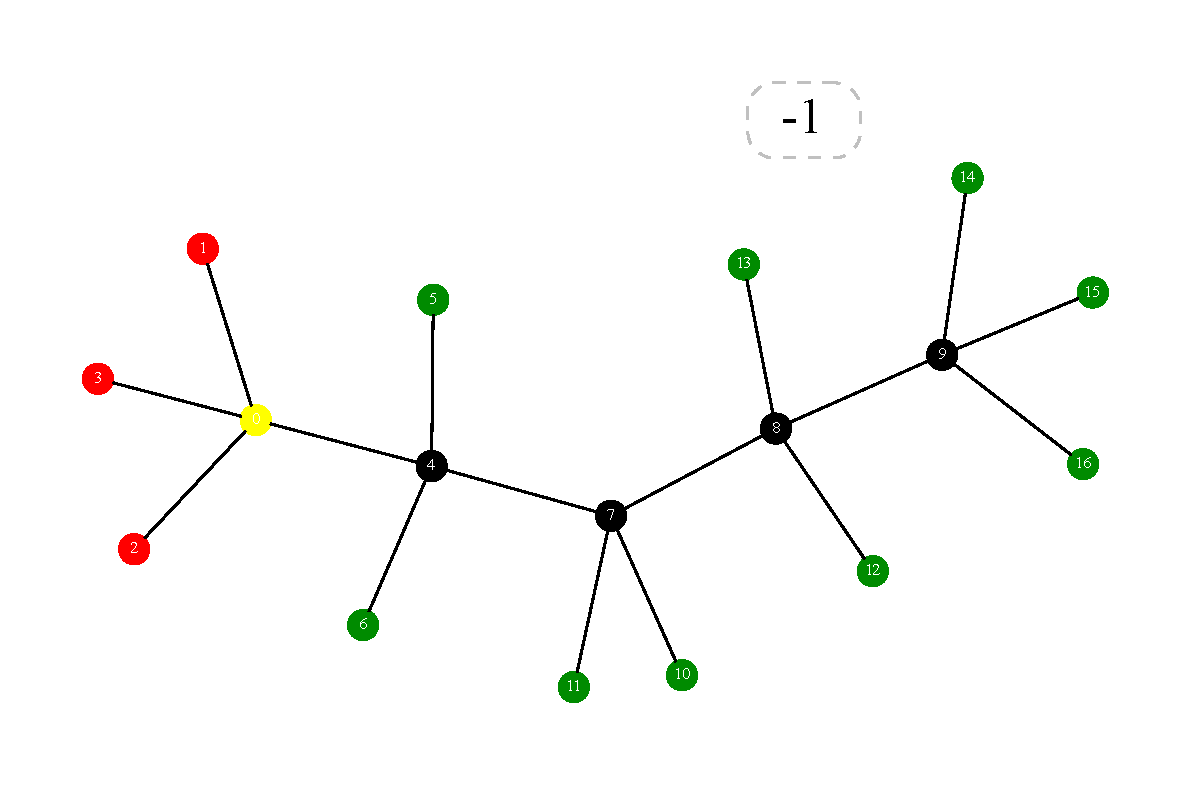
\includegraphics[scale=0.15]{mol_pictures/83.pdf}}
\xrightarrow[0.41]{4.14}
48
\raisebox{-.5\height}{\includegraphics[scale=0.15]{mol_pictures/48.pdf}}
+
61
\raisebox{-.5\height}{\includegraphics[scale=0.15]{mol_pictures/61.pdf}}
$$


reactant bonds broken:\begin{verbatim}
[(0, 0), (0, 11)]
\end{verbatim}
product bonds broken:\begin{verbatim}
[(1, 2), (1, 17)]
\end{verbatim}




\vspace{1cm}
\begin{verbatim}
more than one reactant
fragment matching found
free_energy dG is above threshold=0.0
Terminal.KEEP
\end{verbatim}
$$
81
\raisebox{-.5\height}{\includegraphics[scale=0.15]{mol_pictures/81.pdf}}
+
87
\raisebox{-.5\height}{\includegraphics[scale=0.15]{mol_pictures/87.pdf}}
\xrightarrow[0.27]{2.70}
48
\raisebox{-.5\height}{\includegraphics[scale=0.15]{mol_pictures/48.pdf}}
+
68
\raisebox{-.5\height}{\includegraphics[scale=0.15]{mol_pictures/68.pdf}}
$$


reactant bonds broken:\begin{verbatim}
[(0, 0), (0, 11)]
\end{verbatim}
product bonds broken:\begin{verbatim}
[(1, 9), (1, 10)]
\end{verbatim}




\vspace{1cm}
\begin{verbatim}
more than one reactant
fragment matching found
free_energy dG is above threshold=0.0
Terminal.KEEP
\end{verbatim}
$$
73
\raisebox{-.5\height}{\includegraphics[scale=0.15]{mol_pictures/73.pdf}}
+
88
\raisebox{-.5\height}{\includegraphics[scale=0.15]{mol_pictures/88.pdf}}
\xrightarrow[0.06]{0.57}
54
\raisebox{-.5\height}{\includegraphics[scale=0.15]{mol_pictures/54.pdf}}
+
70
\raisebox{-.5\height}{\includegraphics[scale=0.15]{mol_pictures/70.pdf}}
$$


reactant bonds broken:\begin{verbatim}
[(0, 3), (0, 10)]
\end{verbatim}
product bonds broken:\begin{verbatim}
[(1, 9), (1, 10)]
\end{verbatim}




\vspace{1cm}
\begin{verbatim}
more than one reactant
fragment matching found
free_energy dG is above threshold=0.0
Terminal.KEEP
\end{verbatim}
$$
46
\raisebox{-.5\height}{\includegraphics[scale=0.15]{mol_pictures/46.pdf}}
+
81
\raisebox{-.5\height}{\includegraphics[scale=0.15]{mol_pictures/81.pdf}}
\xrightarrow[0.25]{2.53}
48
\raisebox{-.5\height}{\includegraphics[scale=0.15]{mol_pictures/48.pdf}}
+
75
\raisebox{-.5\height}{\includegraphics[scale=0.15]{mol_pictures/75.pdf}}
$$


reactant bonds broken:\begin{verbatim}
[(1, 0), (1, 11)]
\end{verbatim}
product bonds broken:\begin{verbatim}
[(1, 0), (1, 1)]
\end{verbatim}




\vspace{1cm}
\begin{verbatim}
more than one reactant
fragment matching found
free_energy dG is above threshold=0.0
Terminal.KEEP
\end{verbatim}
$$
46
\raisebox{-.5\height}{\includegraphics[scale=0.15]{mol_pictures/46.pdf}}
+
82
\raisebox{-.5\height}{\includegraphics[scale=0.15]{mol_pictures/82.pdf}}
\xrightarrow[0.33]{3.32}
48
\raisebox{-.5\height}{\includegraphics[scale=0.15]{mol_pictures/48.pdf}}
+
76
\raisebox{-.5\height}{\includegraphics[scale=0.15]{mol_pictures/76.pdf}}
$$


reactant bonds broken:\begin{verbatim}
[(1, 0), (1, 11)]
\end{verbatim}
product bonds broken:\begin{verbatim}
[(1, 0), (1, 1)]
\end{verbatim}




\vspace{1cm}
\begin{verbatim}
more than one reactant
fragment matching found
free_energy dG is above threshold=0.0
Terminal.KEEP
\end{verbatim}
$$
46
\raisebox{-.5\height}{\includegraphics[scale=0.15]{mol_pictures/46.pdf}}
+
82
\raisebox{-.5\height}{\includegraphics[scale=0.15]{mol_pictures/82.pdf}}
\xrightarrow[0.39]{3.88}
50
\raisebox{-.5\height}{\includegraphics[scale=0.15]{mol_pictures/50.pdf}}
+
74
\raisebox{-.5\height}{\includegraphics[scale=0.15]{mol_pictures/74.pdf}}
$$


reactant bonds broken:\begin{verbatim}
[(1, 0), (1, 11)]
\end{verbatim}
product bonds broken:\begin{verbatim}
[(1, 0), (1, 1)]
\end{verbatim}




\vspace{1cm}
\begin{verbatim}
more than one reactant
fragment matching found
free_energy dG is above threshold=0.0
Terminal.KEEP
\end{verbatim}
$$
47
\raisebox{-.5\height}{\includegraphics[scale=0.15]{mol_pictures/47.pdf}}
+
82
\raisebox{-.5\height}{\includegraphics[scale=0.15]{mol_pictures/82.pdf}}
\xrightarrow[0.11]{1.08}
49
\raisebox{-.5\height}{\includegraphics[scale=0.15]{mol_pictures/49.pdf}}
+
76
\raisebox{-.5\height}{\includegraphics[scale=0.15]{mol_pictures/76.pdf}}
$$


reactant bonds broken:\begin{verbatim}
[(1, 0), (1, 11)]
\end{verbatim}
product bonds broken:\begin{verbatim}
[(1, 0), (1, 1)]
\end{verbatim}




\vspace{1cm}
\begin{verbatim}
more than one reactant
fragment matching found
free_energy dG is above threshold=0.0
Terminal.KEEP
\end{verbatim}
$$
46
\raisebox{-.5\height}{\includegraphics[scale=0.15]{mol_pictures/46.pdf}}
+
67
\raisebox{-.5\height}{\includegraphics[scale=0.15]{mol_pictures/67.pdf}}
\xrightarrow[0.05]{0.52}
75
\raisebox{-.5\height}{\includegraphics[scale=0.15]{mol_pictures/75.pdf}}
+
87
\raisebox{-.5\height}{\includegraphics[scale=0.15]{mol_pictures/87.pdf}}
$$


reactant bonds broken:\begin{verbatim}
[(1, 12), (1, 13)]
\end{verbatim}
product bonds broken:\begin{verbatim}
[(0, 0), (0, 1)]
\end{verbatim}




\vspace{1cm}
\begin{verbatim}
more than one reactant
fragment matching found
free_energy dG is above threshold=0.0
Terminal.KEEP
\end{verbatim}
$$
46
\raisebox{-.5\height}{\includegraphics[scale=0.15]{mol_pictures/46.pdf}}
+
69
\raisebox{-.5\height}{\includegraphics[scale=0.15]{mol_pictures/69.pdf}}
\xrightarrow[0.37]{3.69}
74
\raisebox{-.5\height}{\includegraphics[scale=0.15]{mol_pictures/74.pdf}}
+
89
\raisebox{-.5\height}{\includegraphics[scale=0.15]{mol_pictures/89.pdf}}
$$


reactant bonds broken:\begin{verbatim}
[(1, 12), (1, 13)]
\end{verbatim}
product bonds broken:\begin{verbatim}
[(0, 0), (0, 1)]
\end{verbatim}




\vspace{1cm}
\begin{verbatim}
more than one reactant
fragment matching found
free_energy dG is above threshold=0.0
Terminal.KEEP
\end{verbatim}
$$
75
\raisebox{-.5\height}{\includegraphics[scale=0.15]{mol_pictures/75.pdf}}
+
83
\raisebox{-.5\height}{\includegraphics[scale=0.15]{mol_pictures/83.pdf}}
\xrightarrow[0.16]{1.61}
46
\raisebox{-.5\height}{\includegraphics[scale=0.15]{mol_pictures/46.pdf}}
+
61
\raisebox{-.5\height}{\includegraphics[scale=0.15]{mol_pictures/61.pdf}}
$$


reactant bonds broken:\begin{verbatim}
[(0, 0), (0, 1)]
\end{verbatim}
product bonds broken:\begin{verbatim}
[(1, 2), (1, 17)]
\end{verbatim}




\vspace{1cm}
\begin{verbatim}
more than one reactant
fragment matching found
free_energy dG is above threshold=0.0
Terminal.KEEP
\end{verbatim}
$$
46
\raisebox{-.5\height}{\includegraphics[scale=0.15]{mol_pictures/46.pdf}}
+
69
\raisebox{-.5\height}{\includegraphics[scale=0.15]{mol_pictures/69.pdf}}
\xrightarrow[0.23]{2.27}
76
\raisebox{-.5\height}{\includegraphics[scale=0.15]{mol_pictures/76.pdf}}
+
87
\raisebox{-.5\height}{\includegraphics[scale=0.15]{mol_pictures/87.pdf}}
$$


reactant bonds broken:\begin{verbatim}
[(1, 12), (1, 13)]
\end{verbatim}
product bonds broken:\begin{verbatim}
[(0, 0), (0, 1)]
\end{verbatim}




\vspace{1cm}
\begin{verbatim}
more than one reactant
fragment matching found
free_energy dG is above threshold=0.0
Terminal.KEEP
\end{verbatim}
$$
46
\raisebox{-.5\height}{\includegraphics[scale=0.15]{mol_pictures/46.pdf}}
+
70
\raisebox{-.5\height}{\includegraphics[scale=0.15]{mol_pictures/70.pdf}}
\xrightarrow[0.25]{2.52}
74
\raisebox{-.5\height}{\includegraphics[scale=0.15]{mol_pictures/74.pdf}}
+
89
\raisebox{-.5\height}{\includegraphics[scale=0.15]{mol_pictures/89.pdf}}
$$


reactant bonds broken:\begin{verbatim}
[(1, 9), (1, 10)]
\end{verbatim}
product bonds broken:\begin{verbatim}
[(0, 0), (0, 1)]
\end{verbatim}




\vspace{1cm}
\begin{verbatim}
more than one reactant
fragment matching found
free_energy dG is above threshold=0.0
Terminal.KEEP
\end{verbatim}
$$
82
\raisebox{-.5\height}{\includegraphics[scale=0.15]{mol_pictures/82.pdf}}
+
87
\raisebox{-.5\height}{\includegraphics[scale=0.15]{mol_pictures/87.pdf}}
\xrightarrow[0.11]{1.05}
48
\raisebox{-.5\height}{\includegraphics[scale=0.15]{mol_pictures/48.pdf}}
+
69
\raisebox{-.5\height}{\includegraphics[scale=0.15]{mol_pictures/69.pdf}}
$$


reactant bonds broken:\begin{verbatim}
[(0, 0), (0, 11)]
\end{verbatim}
product bonds broken:\begin{verbatim}
[(1, 12), (1, 13)]
\end{verbatim}




\vspace{1cm}
\begin{verbatim}
more than one reactant
fragment matching found
free_energy dG is above threshold=0.0
Terminal.KEEP
\end{verbatim}
$$
46
\raisebox{-.5\height}{\includegraphics[scale=0.15]{mol_pictures/46.pdf}}
+
70
\raisebox{-.5\height}{\includegraphics[scale=0.15]{mol_pictures/70.pdf}}
\xrightarrow[0.11]{1.10}
76
\raisebox{-.5\height}{\includegraphics[scale=0.15]{mol_pictures/76.pdf}}
+
87
\raisebox{-.5\height}{\includegraphics[scale=0.15]{mol_pictures/87.pdf}}
$$


reactant bonds broken:\begin{verbatim}
[(1, 9), (1, 10)]
\end{verbatim}
product bonds broken:\begin{verbatim}
[(0, 0), (0, 1)]
\end{verbatim}




\vspace{1cm}
\begin{verbatim}
more than one reactant
fragment matching found
free_energy dG is above threshold=0.0
Terminal.KEEP
\end{verbatim}
$$
82
\raisebox{-.5\height}{\includegraphics[scale=0.15]{mol_pictures/82.pdf}}
+
87
\raisebox{-.5\height}{\includegraphics[scale=0.15]{mol_pictures/87.pdf}}
\xrightarrow[0.22]{2.22}
48
\raisebox{-.5\height}{\includegraphics[scale=0.15]{mol_pictures/48.pdf}}
+
70
\raisebox{-.5\height}{\includegraphics[scale=0.15]{mol_pictures/70.pdf}}
$$


reactant bonds broken:\begin{verbatim}
[(0, 0), (0, 11)]
\end{verbatim}
product bonds broken:\begin{verbatim}
[(1, 9), (1, 10)]
\end{verbatim}




\vspace{1cm}
\begin{verbatim}
more than one reactant
fragment matching found
free_energy dG is above threshold=0.0
Terminal.KEEP
\end{verbatim}
$$
47
\raisebox{-.5\height}{\includegraphics[scale=0.15]{mol_pictures/47.pdf}}
+
69
\raisebox{-.5\height}{\includegraphics[scale=0.15]{mol_pictures/69.pdf}}
\xrightarrow[0.08]{0.79}
76
\raisebox{-.5\height}{\includegraphics[scale=0.15]{mol_pictures/76.pdf}}
+
88
\raisebox{-.5\height}{\includegraphics[scale=0.15]{mol_pictures/88.pdf}}
$$


reactant bonds broken:\begin{verbatim}
[(1, 12), (1, 13)]
\end{verbatim}
product bonds broken:\begin{verbatim}
[(0, 0), (0, 1)]
\end{verbatim}




\vspace{1cm}
\begin{verbatim}
more than one reactant
fragment matching found
free_energy dG is above threshold=0.0
Terminal.KEEP
\end{verbatim}
$$
82
\raisebox{-.5\height}{\includegraphics[scale=0.15]{mol_pictures/82.pdf}}
+
87
\raisebox{-.5\height}{\includegraphics[scale=0.15]{mol_pictures/87.pdf}}
\xrightarrow[0.33]{3.30}
50
\raisebox{-.5\height}{\includegraphics[scale=0.15]{mol_pictures/50.pdf}}
+
65
\raisebox{-.5\height}{\includegraphics[scale=0.15]{mol_pictures/65.pdf}}
$$


reactant bonds broken:\begin{verbatim}
[(0, 0), (0, 11)]
\end{verbatim}
product bonds broken:\begin{verbatim}
[(1, 12), (1, 13)]
\end{verbatim}




\vspace{1cm}
\begin{verbatim}
more than one reactant
fragment matching found
free_energy dG is above threshold=0.0
Terminal.KEEP
\end{verbatim}
$$
44
\raisebox{-.5\height}{\includegraphics[scale=0.15]{mol_pictures/44.pdf}}
+
87
\raisebox{-.5\height}{\includegraphics[scale=0.15]{mol_pictures/87.pdf}}
\xrightarrow[0.11]{1.07}
67
\raisebox{-.5\height}{\includegraphics[scale=0.15]{mol_pictures/67.pdf}}
+
85
\raisebox{-.5\height}{\includegraphics[scale=0.15]{mol_pictures/85.pdf}}
$$


reactant bonds broken:\begin{verbatim}
[(0, 0), (0, 1)]
\end{verbatim}
product bonds broken:\begin{verbatim}
[(0, 12), (0, 13)]
\end{verbatim}




\vspace{1cm}
\begin{verbatim}
more than one reactant
fragment matching found
free_energy dG is above threshold=0.0
Terminal.KEEP
\end{verbatim}
$$
82
\raisebox{-.5\height}{\includegraphics[scale=0.15]{mol_pictures/82.pdf}}
+
87
\raisebox{-.5\height}{\includegraphics[scale=0.15]{mol_pictures/87.pdf}}
\xrightarrow[0.25]{2.45}
50
\raisebox{-.5\height}{\includegraphics[scale=0.15]{mol_pictures/50.pdf}}
+
66
\raisebox{-.5\height}{\includegraphics[scale=0.15]{mol_pictures/66.pdf}}
$$


reactant bonds broken:\begin{verbatim}
[(0, 0), (0, 11)]
\end{verbatim}
product bonds broken:\begin{verbatim}
[(1, 9), (1, 10)]
\end{verbatim}




\vspace{1cm}
\begin{verbatim}
more than one reactant
fragment matching found
free_energy dG is above threshold=0.0
Terminal.KEEP
\end{verbatim}
$$
44
\raisebox{-.5\height}{\includegraphics[scale=0.15]{mol_pictures/44.pdf}}
+
87
\raisebox{-.5\height}{\includegraphics[scale=0.15]{mol_pictures/87.pdf}}
\xrightarrow[0.18]{1.75}
68
\raisebox{-.5\height}{\includegraphics[scale=0.15]{mol_pictures/68.pdf}}
+
85
\raisebox{-.5\height}{\includegraphics[scale=0.15]{mol_pictures/85.pdf}}
$$


reactant bonds broken:\begin{verbatim}
[(0, 0), (0, 1)]
\end{verbatim}
product bonds broken:\begin{verbatim}
[(0, 9), (0, 10)]
\end{verbatim}




\vspace{1cm}
\begin{verbatim}
more than one reactant
fragment matching found
free_energy dG is above threshold=0.0
Terminal.KEEP
\end{verbatim}
$$
82
\raisebox{-.5\height}{\includegraphics[scale=0.15]{mol_pictures/82.pdf}}
+
88
\raisebox{-.5\height}{\includegraphics[scale=0.15]{mol_pictures/88.pdf}}
\xrightarrow[0.03]{0.29}
49
\raisebox{-.5\height}{\includegraphics[scale=0.15]{mol_pictures/49.pdf}}
+
69
\raisebox{-.5\height}{\includegraphics[scale=0.15]{mol_pictures/69.pdf}}
$$


reactant bonds broken:\begin{verbatim}
[(0, 0), (0, 11)]
\end{verbatim}
product bonds broken:\begin{verbatim}
[(1, 12), (1, 13)]
\end{verbatim}




\vspace{1cm}
\begin{verbatim}
more than one reactant
fragment matching found
free_energy dG is above threshold=0.0
Terminal.KEEP
\end{verbatim}
$$
82
\raisebox{-.5\height}{\includegraphics[scale=0.15]{mol_pictures/82.pdf}}
+
88
\raisebox{-.5\height}{\includegraphics[scale=0.15]{mol_pictures/88.pdf}}
\xrightarrow[0.15]{1.46}
49
\raisebox{-.5\height}{\includegraphics[scale=0.15]{mol_pictures/49.pdf}}
+
70
\raisebox{-.5\height}{\includegraphics[scale=0.15]{mol_pictures/70.pdf}}
$$


reactant bonds broken:\begin{verbatim}
[(0, 0), (0, 11)]
\end{verbatim}
product bonds broken:\begin{verbatim}
[(1, 9), (1, 10)]
\end{verbatim}




\vspace{1cm}
\begin{verbatim}
more than one reactant
fragment matching found
free_energy dG is above threshold=0.0
Terminal.KEEP
\end{verbatim}
$$
75
\raisebox{-.5\height}{\includegraphics[scale=0.15]{mol_pictures/75.pdf}}
+
87
\raisebox{-.5\height}{\includegraphics[scale=0.15]{mol_pictures/87.pdf}}
\xrightarrow[0.02]{0.16}
46
\raisebox{-.5\height}{\includegraphics[scale=0.15]{mol_pictures/46.pdf}}
+
68
\raisebox{-.5\height}{\includegraphics[scale=0.15]{mol_pictures/68.pdf}}
$$


reactant bonds broken:\begin{verbatim}
[(0, 0), (0, 1)]
\end{verbatim}
product bonds broken:\begin{verbatim}
[(1, 9), (1, 10)]
\end{verbatim}




\vspace{1cm}
\begin{verbatim}
more than one reactant
fragment matching found
free_energy dG is above threshold=0.0
Terminal.KEEP
\end{verbatim}
$$
82
\raisebox{-.5\height}{\includegraphics[scale=0.15]{mol_pictures/82.pdf}}
+
88
\raisebox{-.5\height}{\includegraphics[scale=0.15]{mol_pictures/88.pdf}}
\xrightarrow[0.02]{0.24}
50
\raisebox{-.5\height}{\includegraphics[scale=0.15]{mol_pictures/50.pdf}}
+
67
\raisebox{-.5\height}{\includegraphics[scale=0.15]{mol_pictures/67.pdf}}
$$


reactant bonds broken:\begin{verbatim}
[(0, 0), (0, 11)]
\end{verbatim}
product bonds broken:\begin{verbatim}
[(1, 12), (1, 13)]
\end{verbatim}




\vspace{1cm}
\begin{verbatim}
more than one reactant
fragment matching found
free_energy dG is above threshold=0.0
Terminal.KEEP
\end{verbatim}
$$
69
\raisebox{-.5\height}{\includegraphics[scale=0.15]{mol_pictures/69.pdf}}
+
85
\raisebox{-.5\height}{\includegraphics[scale=0.15]{mol_pictures/85.pdf}}
\xrightarrow[0.24]{2.43}
43
\raisebox{-.5\height}{\includegraphics[scale=0.15]{mol_pictures/43.pdf}}
+
89
\raisebox{-.5\height}{\includegraphics[scale=0.15]{mol_pictures/89.pdf}}
$$


reactant bonds broken:\begin{verbatim}
[(0, 12), (0, 13)]
\end{verbatim}
product bonds broken:\begin{verbatim}
[(0, 0), (0, 1)]
\end{verbatim}




\vspace{1cm}
\begin{verbatim}
more than one reactant
fragment matching found
free_energy dG is above threshold=0.0
Terminal.KEEP
\end{verbatim}
$$
82
\raisebox{-.5\height}{\includegraphics[scale=0.15]{mol_pictures/82.pdf}}
+
88
\raisebox{-.5\height}{\includegraphics[scale=0.15]{mol_pictures/88.pdf}}
\xrightarrow[0.09]{0.92}
50
\raisebox{-.5\height}{\includegraphics[scale=0.15]{mol_pictures/50.pdf}}
+
68
\raisebox{-.5\height}{\includegraphics[scale=0.15]{mol_pictures/68.pdf}}
$$


reactant bonds broken:\begin{verbatim}
[(0, 0), (0, 11)]
\end{verbatim}
product bonds broken:\begin{verbatim}
[(1, 9), (1, 10)]
\end{verbatim}




\vspace{1cm}
\begin{verbatim}
more than one reactant
fragment matching found
free_energy dG is above threshold=0.0
Terminal.KEEP
\end{verbatim}
$$
69
\raisebox{-.5\height}{\includegraphics[scale=0.15]{mol_pictures/69.pdf}}
+
85
\raisebox{-.5\height}{\includegraphics[scale=0.15]{mol_pictures/85.pdf}}
\xrightarrow[0.25]{2.53}
45
\raisebox{-.5\height}{\includegraphics[scale=0.15]{mol_pictures/45.pdf}}
+
87
\raisebox{-.5\height}{\includegraphics[scale=0.15]{mol_pictures/87.pdf}}
$$


reactant bonds broken:\begin{verbatim}
[(0, 12), (0, 13)]
\end{verbatim}
product bonds broken:\begin{verbatim}
[(0, 0), (0, 1)]
\end{verbatim}




\vspace{1cm}
\begin{verbatim}
more than one reactant
fragment matching found
free_energy dG is above threshold=0.0
Terminal.KEEP
\end{verbatim}
$$
44
\raisebox{-.5\height}{\includegraphics[scale=0.15]{mol_pictures/44.pdf}}
+
83
\raisebox{-.5\height}{\includegraphics[scale=0.15]{mol_pictures/83.pdf}}
\xrightarrow[0.32]{3.20}
61
\raisebox{-.5\height}{\includegraphics[scale=0.15]{mol_pictures/61.pdf}}
+
85
\raisebox{-.5\height}{\includegraphics[scale=0.15]{mol_pictures/85.pdf}}
$$


reactant bonds broken:\begin{verbatim}
[(0, 0), (0, 1)]
\end{verbatim}
product bonds broken:\begin{verbatim}
[(0, 2), (0, 17)]
\end{verbatim}




\vspace{1cm}
\begin{verbatim}
more than one reactant
fragment matching found
free_energy dG is above threshold=0.0
Terminal.KEEP
\end{verbatim}
$$
69
\raisebox{-.5\height}{\includegraphics[scale=0.15]{mol_pictures/69.pdf}}
+
86
\raisebox{-.5\height}{\includegraphics[scale=0.15]{mol_pictures/86.pdf}}
\xrightarrow[0.21]{2.06}
45
\raisebox{-.5\height}{\includegraphics[scale=0.15]{mol_pictures/45.pdf}}
+
88
\raisebox{-.5\height}{\includegraphics[scale=0.15]{mol_pictures/88.pdf}}
$$


reactant bonds broken:\begin{verbatim}
[(0, 12), (0, 13)]
\end{verbatim}
product bonds broken:\begin{verbatim}
[(0, 0), (0, 1)]
\end{verbatim}




\vspace{1cm}
\begin{verbatim}
more than one reactant
fragment matching found
free_energy dG is above threshold=0.0
Terminal.KEEP
\end{verbatim}
$$
76
\raisebox{-.5\height}{\includegraphics[scale=0.15]{mol_pictures/76.pdf}}
+
88
\raisebox{-.5\height}{\includegraphics[scale=0.15]{mol_pictures/88.pdf}}
\xrightarrow[0.04]{0.38}
47
\raisebox{-.5\height}{\includegraphics[scale=0.15]{mol_pictures/47.pdf}}
+
70
\raisebox{-.5\height}{\includegraphics[scale=0.15]{mol_pictures/70.pdf}}
$$


reactant bonds broken:\begin{verbatim}
[(0, 0), (0, 1)]
\end{verbatim}
product bonds broken:\begin{verbatim}
[(1, 9), (1, 10)]
\end{verbatim}




\vspace{1cm}
\begin{verbatim}
more than one reactant
fragment matching found
free_energy dG is above threshold=0.0
Terminal.KEEP
\end{verbatim}
$$
70
\raisebox{-.5\height}{\includegraphics[scale=0.15]{mol_pictures/70.pdf}}
+
85
\raisebox{-.5\height}{\includegraphics[scale=0.15]{mol_pictures/85.pdf}}
\xrightarrow[0.13]{1.26}
43
\raisebox{-.5\height}{\includegraphics[scale=0.15]{mol_pictures/43.pdf}}
+
89
\raisebox{-.5\height}{\includegraphics[scale=0.15]{mol_pictures/89.pdf}}
$$


reactant bonds broken:\begin{verbatim}
[(0, 9), (0, 10)]
\end{verbatim}
product bonds broken:\begin{verbatim}
[(0, 0), (0, 1)]
\end{verbatim}




\vspace{1cm}
\begin{verbatim}
more than one reactant
fragment matching found
free_energy dG is above threshold=0.0
Terminal.KEEP
\end{verbatim}
$$
81
\raisebox{-.5\height}{\includegraphics[scale=0.15]{mol_pictures/81.pdf}}
+
85
\raisebox{-.5\height}{\includegraphics[scale=0.15]{mol_pictures/85.pdf}}
\xrightarrow[0.09]{0.94}
44
\raisebox{-.5\height}{\includegraphics[scale=0.15]{mol_pictures/44.pdf}}
+
48
\raisebox{-.5\height}{\includegraphics[scale=0.15]{mol_pictures/48.pdf}}
$$


reactant bonds broken:\begin{verbatim}
[(0, 0), (0, 11)]
\end{verbatim}
product bonds broken:\begin{verbatim}
[(0, 0), (0, 1)]
\end{verbatim}




\vspace{1cm}
\begin{verbatim}
more than one reactant
fragment matching found
free_energy dG is above threshold=0.0
Terminal.KEEP
\end{verbatim}
$$
70
\raisebox{-.5\height}{\includegraphics[scale=0.15]{mol_pictures/70.pdf}}
+
85
\raisebox{-.5\height}{\includegraphics[scale=0.15]{mol_pictures/85.pdf}}
\xrightarrow[0.14]{1.36}
45
\raisebox{-.5\height}{\includegraphics[scale=0.15]{mol_pictures/45.pdf}}
+
87
\raisebox{-.5\height}{\includegraphics[scale=0.15]{mol_pictures/87.pdf}}
$$


reactant bonds broken:\begin{verbatim}
[(0, 9), (0, 10)]
\end{verbatim}
product bonds broken:\begin{verbatim}
[(0, 0), (0, 1)]
\end{verbatim}




\vspace{1cm}
\begin{verbatim}
more than one reactant
fragment matching found
free_energy dG is above threshold=0.0
Terminal.KEEP
\end{verbatim}
$$
82
\raisebox{-.5\height}{\includegraphics[scale=0.15]{mol_pictures/82.pdf}}
+
85
\raisebox{-.5\height}{\includegraphics[scale=0.15]{mol_pictures/85.pdf}}
\xrightarrow[0.26]{2.62}
43
\raisebox{-.5\height}{\includegraphics[scale=0.15]{mol_pictures/43.pdf}}
+
50
\raisebox{-.5\height}{\includegraphics[scale=0.15]{mol_pictures/50.pdf}}
$$


reactant bonds broken:\begin{verbatim}
[(0, 0), (0, 11)]
\end{verbatim}
product bonds broken:\begin{verbatim}
[(0, 0), (0, 1)]
\end{verbatim}




\vspace{1cm}
\begin{verbatim}
more than one reactant
fragment matching found
free_energy dG is above threshold=0.0
Terminal.KEEP
\end{verbatim}
$$
82
\raisebox{-.5\height}{\includegraphics[scale=0.15]{mol_pictures/82.pdf}}
+
85
\raisebox{-.5\height}{\includegraphics[scale=0.15]{mol_pictures/85.pdf}}
\xrightarrow[0.36]{3.58}
45
\raisebox{-.5\height}{\includegraphics[scale=0.15]{mol_pictures/45.pdf}}
+
48
\raisebox{-.5\height}{\includegraphics[scale=0.15]{mol_pictures/48.pdf}}
$$


reactant bonds broken:\begin{verbatim}
[(0, 0), (0, 11)]
\end{verbatim}
product bonds broken:\begin{verbatim}
[(0, 0), (0, 1)]
\end{verbatim}




\vspace{1cm}
\begin{verbatim}
more than one reactant
fragment matching found
free_energy dG is above threshold=0.0
Terminal.KEEP
\end{verbatim}
$$
82
\raisebox{-.5\height}{\includegraphics[scale=0.15]{mol_pictures/82.pdf}}
+
86
\raisebox{-.5\height}{\includegraphics[scale=0.15]{mol_pictures/86.pdf}}
\xrightarrow[0.24]{2.35}
45
\raisebox{-.5\height}{\includegraphics[scale=0.15]{mol_pictures/45.pdf}}
+
49
\raisebox{-.5\height}{\includegraphics[scale=0.15]{mol_pictures/49.pdf}}
$$


reactant bonds broken:\begin{verbatim}
[(0, 0), (0, 11)]
\end{verbatim}
product bonds broken:\begin{verbatim}
[(0, 0), (0, 1)]
\end{verbatim}




\vspace{1cm}
\begin{verbatim}
more than one reactant
fragment matching found
free_energy dG is above threshold=0.0
Terminal.KEEP
\end{verbatim}
$$
44
\raisebox{-.5\height}{\includegraphics[scale=0.15]{mol_pictures/44.pdf}}
+
46
\raisebox{-.5\height}{\includegraphics[scale=0.15]{mol_pictures/46.pdf}}
\xrightarrow[0.16]{1.59}
75
\raisebox{-.5\height}{\includegraphics[scale=0.15]{mol_pictures/75.pdf}}
+
85
\raisebox{-.5\height}{\includegraphics[scale=0.15]{mol_pictures/85.pdf}}
$$


reactant bonds broken:\begin{verbatim}
[(0, 0), (0, 1)]
\end{verbatim}
product bonds broken:\begin{verbatim}
[(0, 0), (0, 1)]
\end{verbatim}




\vspace{1cm}
\begin{verbatim}
more than one reactant
fragment matching found
free_energy dG is above threshold=0.0
Terminal.KEEP
\end{verbatim}
$$
70
\raisebox{-.5\height}{\includegraphics[scale=0.15]{mol_pictures/70.pdf}}
+
86
\raisebox{-.5\height}{\includegraphics[scale=0.15]{mol_pictures/86.pdf}}
\xrightarrow[0.09]{0.89}
45
\raisebox{-.5\height}{\includegraphics[scale=0.15]{mol_pictures/45.pdf}}
+
88
\raisebox{-.5\height}{\includegraphics[scale=0.15]{mol_pictures/88.pdf}}
$$


reactant bonds broken:\begin{verbatim}
[(0, 9), (0, 10)]
\end{verbatim}
product bonds broken:\begin{verbatim}
[(0, 0), (0, 1)]
\end{verbatim}




\vspace{1cm}
\begin{verbatim}
more than one reactant
fragment matching found
free_energy dG is above threshold=0.0
Terminal.KEEP
\end{verbatim}
$$
76
\raisebox{-.5\height}{\includegraphics[scale=0.15]{mol_pictures/76.pdf}}
+
85
\raisebox{-.5\height}{\includegraphics[scale=0.15]{mol_pictures/85.pdf}}
\xrightarrow[0.03]{0.26}
45
\raisebox{-.5\height}{\includegraphics[scale=0.15]{mol_pictures/45.pdf}}
+
46
\raisebox{-.5\height}{\includegraphics[scale=0.15]{mol_pictures/46.pdf}}
$$


reactant bonds broken:\begin{verbatim}
[(0, 0), (0, 1)]
\end{verbatim}
product bonds broken:\begin{verbatim}
[(0, 0), (0, 1)]
\end{verbatim}




\vspace{1cm}
\begin{verbatim}
more than one reactant
fragment matching found
free_energy dG is above threshold=0.0
Terminal.KEEP
\end{verbatim}
$$
76
\raisebox{-.5\height}{\includegraphics[scale=0.15]{mol_pictures/76.pdf}}
+
86
\raisebox{-.5\height}{\includegraphics[scale=0.15]{mol_pictures/86.pdf}}
\xrightarrow[0.13]{1.27}
45
\raisebox{-.5\height}{\includegraphics[scale=0.15]{mol_pictures/45.pdf}}
+
47
\raisebox{-.5\height}{\includegraphics[scale=0.15]{mol_pictures/47.pdf}}
$$


reactant bonds broken:\begin{verbatim}
[(0, 0), (0, 1)]
\end{verbatim}
product bonds broken:\begin{verbatim}
[(0, 0), (0, 1)]
\end{verbatim}




\vspace{1cm}
\begin{verbatim}
more than one reactant
fragment matching found
free_energy dG is above threshold=0.0
Terminal.KEEP
\end{verbatim}
$$
41
\raisebox{-.5\height}{\includegraphics[scale=0.15]{mol_pictures/41.pdf}}
+
85
\raisebox{-.5\height}{\includegraphics[scale=0.15]{mol_pictures/85.pdf}}
\xrightarrow[0.05]{0.50}
43
\raisebox{-.5\height}{\includegraphics[scale=0.15]{mol_pictures/43.pdf}}
+
68
\raisebox{-.5\height}{\includegraphics[scale=0.15]{mol_pictures/68.pdf}}
$$


reactant bonds broken:\begin{verbatim}
[(0, 12), (0, 13)]
\end{verbatim}
product bonds broken:\begin{verbatim}
[(0, 0), (0, 1)]
\end{verbatim}




\vspace{1cm}
\begin{verbatim}
more than one reactant
fragment matching found
free_energy dG is above threshold=0.0
Terminal.KEEP
\end{verbatim}
$$
41
\raisebox{-.5\height}{\includegraphics[scale=0.15]{mol_pictures/41.pdf}}
+
87
\raisebox{-.5\height}{\includegraphics[scale=0.15]{mol_pictures/87.pdf}}
\xrightarrow[0.05]{0.50}
65
\raisebox{-.5\height}{\includegraphics[scale=0.15]{mol_pictures/65.pdf}}
+
67
\raisebox{-.5\height}{\includegraphics[scale=0.15]{mol_pictures/67.pdf}}
$$


reactant bonds broken:\begin{verbatim}
[(0, 9), (0, 25)]
\end{verbatim}
product bonds broken:\begin{verbatim}
[(1, 12), (1, 13)]
\end{verbatim}




\vspace{1cm}
\begin{verbatim}
more than one reactant
fragment matching found
free_energy dG is above threshold=0.0
Terminal.KEEP
\end{verbatim}
$$
42
\raisebox{-.5\height}{\includegraphics[scale=0.15]{mol_pictures/42.pdf}}
+
86
\raisebox{-.5\height}{\includegraphics[scale=0.15]{mol_pictures/86.pdf}}
\xrightarrow[0.14]{1.36}
45
\raisebox{-.5\height}{\includegraphics[scale=0.15]{mol_pictures/45.pdf}}
+
67
\raisebox{-.5\height}{\includegraphics[scale=0.15]{mol_pictures/67.pdf}}
$$


reactant bonds broken:\begin{verbatim}
[(0, 9), (0, 25)]
\end{verbatim}
product bonds broken:\begin{verbatim}
[(0, 0), (0, 1)]
\end{verbatim}




\vspace{1cm}
\begin{verbatim}
more than one reactant
fragment matching found
free_energy dG is above threshold=0.0
Terminal.KEEP
\end{verbatim}
$$
41
\raisebox{-.5\height}{\includegraphics[scale=0.15]{mol_pictures/41.pdf}}
+
66
\raisebox{-.5\height}{\includegraphics[scale=0.15]{mol_pictures/66.pdf}}
\xrightarrow[0.02]{0.19}
40
\raisebox{-.5\height}{\includegraphics[scale=0.15]{mol_pictures/40.pdf}}
+
68
\raisebox{-.5\height}{\includegraphics[scale=0.15]{mol_pictures/68.pdf}}
$$


reactant bonds broken:\begin{verbatim}
[(1, 0), (1, 3)]
\end{verbatim}
product bonds broken:\begin{verbatim}
[(1, 0), (1, 1)]
\end{verbatim}




\vspace{1cm}
\begin{verbatim}
more than one reactant
fragment matching found
free_energy dG is above threshold=0.0
Terminal.KEEP
\end{verbatim}
$$
42
\raisebox{-.5\height}{\includegraphics[scale=0.15]{mol_pictures/42.pdf}}
+
86
\raisebox{-.5\height}{\includegraphics[scale=0.15]{mol_pictures/86.pdf}}
\xrightarrow[0.20]{2.05}
45
\raisebox{-.5\height}{\includegraphics[scale=0.15]{mol_pictures/45.pdf}}
+
68
\raisebox{-.5\height}{\includegraphics[scale=0.15]{mol_pictures/68.pdf}}
$$


reactant bonds broken:\begin{verbatim}
[(0, 12), (0, 13)]
\end{verbatim}
product bonds broken:\begin{verbatim}
[(0, 0), (0, 1)]
\end{verbatim}




\vspace{1cm}
\begin{verbatim}
more than one reactant
fragment matching found
free_energy dG is above threshold=0.0
Terminal.KEEP
\end{verbatim}
$$
42
\raisebox{-.5\height}{\includegraphics[scale=0.15]{mol_pictures/42.pdf}}
+
65
\raisebox{-.5\height}{\includegraphics[scale=0.15]{mol_pictures/65.pdf}}
\xrightarrow[0.05]{0.53}
40
\raisebox{-.5\height}{\includegraphics[scale=0.15]{mol_pictures/40.pdf}}
+
69
\raisebox{-.5\height}{\includegraphics[scale=0.15]{mol_pictures/69.pdf}}
$$


reactant bonds broken:\begin{verbatim}
[(1, 0), (1, 3)]
\end{verbatim}
product bonds broken:\begin{verbatim}
[(1, 0), (1, 3)]
\end{verbatim}




\vspace{1cm}
\begin{verbatim}
more than one reactant
fragment matching found
free_energy dG is above threshold=0.0
Terminal.KEEP
\end{verbatim}
$$
41
\raisebox{-.5\height}{\includegraphics[scale=0.15]{mol_pictures/41.pdf}}
+
87
\raisebox{-.5\height}{\includegraphics[scale=0.15]{mol_pictures/87.pdf}}
\xrightarrow[0.12]{1.18}
65
\raisebox{-.5\height}{\includegraphics[scale=0.15]{mol_pictures/65.pdf}}
+
68
\raisebox{-.5\height}{\includegraphics[scale=0.15]{mol_pictures/68.pdf}}
$$


reactant bonds broken:\begin{verbatim}
[(0, 9), (0, 25)]
\end{verbatim}
product bonds broken:\begin{verbatim}
[(1, 9), (1, 10)]
\end{verbatim}




\vspace{1cm}
\begin{verbatim}
more than one reactant
fragment matching found
free_energy dG is above threshold=0.0
Terminal.KEEP
\end{verbatim}
$$
42
\raisebox{-.5\height}{\includegraphics[scale=0.15]{mol_pictures/42.pdf}}
+
65
\raisebox{-.5\height}{\includegraphics[scale=0.15]{mol_pictures/65.pdf}}
\xrightarrow[0.17]{1.69}
40
\raisebox{-.5\height}{\includegraphics[scale=0.15]{mol_pictures/40.pdf}}
+
70
\raisebox{-.5\height}{\includegraphics[scale=0.15]{mol_pictures/70.pdf}}
$$


reactant bonds broken:\begin{verbatim}
[(1, 12), (1, 13)]
\end{verbatim}
product bonds broken:\begin{verbatim}
[(1, 9), (1, 10)]
\end{verbatim}




\vspace{1cm}
\begin{verbatim}
more than one reactant
fragment matching found
free_energy dG is above threshold=0.0
Terminal.KEEP
\end{verbatim}
$$
43
\raisebox{-.5\height}{\includegraphics[scale=0.15]{mol_pictures/43.pdf}}
+
67
\raisebox{-.5\height}{\includegraphics[scale=0.15]{mol_pictures/67.pdf}}
\xrightarrow[0.02]{0.18}
41
\raisebox{-.5\height}{\includegraphics[scale=0.15]{mol_pictures/41.pdf}}
+
85
\raisebox{-.5\height}{\includegraphics[scale=0.15]{mol_pictures/85.pdf}}
$$


reactant bonds broken:\begin{verbatim}
[(0, 0), (0, 1)]
\end{verbatim}
product bonds broken:\begin{verbatim}
[(0, 9), (0, 25)]
\end{verbatim}




\vspace{1cm}
\begin{verbatim}
more than one reactant
fragment matching found
free_energy dG is above threshold=0.0
Terminal.KEEP
\end{verbatim}
$$
42
\raisebox{-.5\height}{\includegraphics[scale=0.15]{mol_pictures/42.pdf}}
+
66
\raisebox{-.5\height}{\includegraphics[scale=0.15]{mol_pictures/66.pdf}}
\xrightarrow[0.14]{1.38}
40
\raisebox{-.5\height}{\includegraphics[scale=0.15]{mol_pictures/40.pdf}}
+
69
\raisebox{-.5\height}{\includegraphics[scale=0.15]{mol_pictures/69.pdf}}
$$


reactant bonds broken:\begin{verbatim}
[(1, 9), (1, 10)]
\end{verbatim}
product bonds broken:\begin{verbatim}
[(1, 12), (1, 13)]
\end{verbatim}




\vspace{1cm}
\begin{verbatim}
more than one reactant
fragment matching found
free_energy dG is above threshold=0.0
Terminal.KEEP
\end{verbatim}
$$
42
\raisebox{-.5\height}{\includegraphics[scale=0.15]{mol_pictures/42.pdf}}
+
66
\raisebox{-.5\height}{\includegraphics[scale=0.15]{mol_pictures/66.pdf}}
\xrightarrow[0.25]{2.54}
40
\raisebox{-.5\height}{\includegraphics[scale=0.15]{mol_pictures/40.pdf}}
+
70
\raisebox{-.5\height}{\includegraphics[scale=0.15]{mol_pictures/70.pdf}}
$$


reactant bonds broken:\begin{verbatim}
[(1, 0), (1, 3)]
\end{verbatim}
product bonds broken:\begin{verbatim}
[(1, 0), (1, 3)]
\end{verbatim}




\vspace{1cm}
\begin{verbatim}
more than one reactant
fragment matching found
free_energy dG is above threshold=0.0
Terminal.KEEP
\end{verbatim}
$$
41
\raisebox{-.5\height}{\includegraphics[scale=0.15]{mol_pictures/41.pdf}}
+
87
\raisebox{-.5\height}{\includegraphics[scale=0.15]{mol_pictures/87.pdf}}
\xrightarrow[0.03]{0.33}
66
\raisebox{-.5\height}{\includegraphics[scale=0.15]{mol_pictures/66.pdf}}
+
68
\raisebox{-.5\height}{\includegraphics[scale=0.15]{mol_pictures/68.pdf}}
$$


reactant bonds broken:\begin{verbatim}
[(0, 12), (0, 13)]
\end{verbatim}
product bonds broken:\begin{verbatim}
[(1, 9), (1, 10)]
\end{verbatim}




\vspace{1cm}
\begin{verbatim}
more than one reactant
fragment matching found
free_energy dG is above threshold=0.0
Terminal.KEEP
\end{verbatim}
$$
44
\raisebox{-.5\height}{\includegraphics[scale=0.15]{mol_pictures/44.pdf}}
+
65
\raisebox{-.5\height}{\includegraphics[scale=0.15]{mol_pictures/65.pdf}}
\xrightarrow[0.06]{0.57}
41
\raisebox{-.5\height}{\includegraphics[scale=0.15]{mol_pictures/41.pdf}}
+
85
\raisebox{-.5\height}{\includegraphics[scale=0.15]{mol_pictures/85.pdf}}
$$


reactant bonds broken:\begin{verbatim}
[(0, 0), (0, 1)]
\end{verbatim}
product bonds broken:\begin{verbatim}
[(0, 9), (0, 25)]
\end{verbatim}




\vspace{1cm}
\begin{verbatim}
more than one reactant
fragment matching found
free_energy dG is above threshold=0.0
Terminal.KEEP
\end{verbatim}
$$
42
\raisebox{-.5\height}{\includegraphics[scale=0.15]{mol_pictures/42.pdf}}
+
67
\raisebox{-.5\height}{\includegraphics[scale=0.15]{mol_pictures/67.pdf}}
\xrightarrow[0.11]{1.13}
68
\raisebox{-.5\height}{\includegraphics[scale=0.15]{mol_pictures/68.pdf}}
+
93
\raisebox{-.5\height}{\includegraphics[scale=0.15]{mol_pictures/93.pdf}}
$$


reactant bonds broken:\begin{verbatim}
[(0, 12), (0, 13)]
\end{verbatim}
product bonds broken:\begin{verbatim}
[(1, 12), (1, 25)]
\end{verbatim}




\vspace{1cm}
\begin{verbatim}
more than one reactant
fragment matching found
free_energy dG is above threshold=0.0
Terminal.KEEP
\end{verbatim}
$$
42
\raisebox{-.5\height}{\includegraphics[scale=0.15]{mol_pictures/42.pdf}}
+
88
\raisebox{-.5\height}{\includegraphics[scale=0.15]{mol_pictures/88.pdf}}
\xrightarrow[0.05]{0.47}
67
\raisebox{-.5\height}{\includegraphics[scale=0.15]{mol_pictures/67.pdf}}
+
70
\raisebox{-.5\height}{\includegraphics[scale=0.15]{mol_pictures/70.pdf}}
$$


reactant bonds broken:\begin{verbatim}
[(0, 9), (0, 25)]
\end{verbatim}
product bonds broken:\begin{verbatim}
[(1, 9), (1, 10)]
\end{verbatim}




\vspace{1cm}
\begin{verbatim}
more than one reactant
fragment matching found
free_energy dG is above threshold=0.0
Terminal.KEEP
\end{verbatim}
$$
44
\raisebox{-.5\height}{\includegraphics[scale=0.15]{mol_pictures/44.pdf}}
+
66
\raisebox{-.5\height}{\includegraphics[scale=0.15]{mol_pictures/66.pdf}}
\xrightarrow[0.14]{1.42}
41
\raisebox{-.5\height}{\includegraphics[scale=0.15]{mol_pictures/41.pdf}}
+
85
\raisebox{-.5\height}{\includegraphics[scale=0.15]{mol_pictures/85.pdf}}
$$


reactant bonds broken:\begin{verbatim}
[(0, 0), (0, 1)]
\end{verbatim}
product bonds broken:\begin{verbatim}
[(0, 12), (0, 13)]
\end{verbatim}




\vspace{1cm}
\begin{verbatim}
more than one reactant
fragment matching found
free_energy dG is above threshold=0.0
Terminal.KEEP
\end{verbatim}
$$
66
\raisebox{-.5\height}{\includegraphics[scale=0.15]{mol_pictures/66.pdf}}
+
93
\raisebox{-.5\height}{\includegraphics[scale=0.15]{mol_pictures/93.pdf}}
\xrightarrow[0.04]{0.40}
42
\raisebox{-.5\height}{\includegraphics[scale=0.15]{mol_pictures/42.pdf}}
+
65
\raisebox{-.5\height}{\includegraphics[scale=0.15]{mol_pictures/65.pdf}}
$$


reactant bonds broken:\begin{verbatim}
[(1, 12), (1, 25)]
\end{verbatim}
product bonds broken:\begin{verbatim}
[(0, 12), (0, 13)]
\end{verbatim}




\vspace{1cm}
\begin{verbatim}
more than one reactant
fragment matching found
free_energy dG is above threshold=0.0
Terminal.KEEP
\end{verbatim}
$$
42
\raisebox{-.5\height}{\includegraphics[scale=0.15]{mol_pictures/42.pdf}}
+
88
\raisebox{-.5\height}{\includegraphics[scale=0.15]{mol_pictures/88.pdf}}
\xrightarrow[0.12]{1.15}
68
\raisebox{-.5\height}{\includegraphics[scale=0.15]{mol_pictures/68.pdf}}
+
70
\raisebox{-.5\height}{\includegraphics[scale=0.15]{mol_pictures/70.pdf}}
$$


reactant bonds broken:\begin{verbatim}
[(0, 12), (0, 13)]
\end{verbatim}
product bonds broken:\begin{verbatim}
[(1, 9), (1, 10)]
\end{verbatim}




\vspace{1cm}
\begin{verbatim}
more than one reactant
fragment matching found
free_energy dG is above threshold=0.0
Terminal.KEEP
\end{verbatim}
$$
86
\raisebox{-.5\height}{\includegraphics[scale=0.15]{mol_pictures/86.pdf}}
+
93
\raisebox{-.5\height}{\includegraphics[scale=0.15]{mol_pictures/93.pdf}}
\xrightarrow[0.09]{0.92}
45
\raisebox{-.5\height}{\includegraphics[scale=0.15]{mol_pictures/45.pdf}}
+
67
\raisebox{-.5\height}{\includegraphics[scale=0.15]{mol_pictures/67.pdf}}
$$


reactant bonds broken:\begin{verbatim}
[(1, 12), (1, 25)]
\end{verbatim}
product bonds broken:\begin{verbatim}
[(0, 0), (0, 1)]
\end{verbatim}




\vspace{1cm}
\begin{verbatim}
more than one reactant
fragment matching found
free_energy dG is above threshold=0.0
Terminal.KEEP
\end{verbatim}
$$
65
\raisebox{-.5\height}{\includegraphics[scale=0.15]{mol_pictures/65.pdf}}
+
81
\raisebox{-.5\height}{\includegraphics[scale=0.15]{mol_pictures/81.pdf}}
\xrightarrow[0.15]{1.51}
41
\raisebox{-.5\height}{\includegraphics[scale=0.15]{mol_pictures/41.pdf}}
+
48
\raisebox{-.5\height}{\includegraphics[scale=0.15]{mol_pictures/48.pdf}}
$$


reactant bonds broken:\begin{verbatim}
[(1, 0), (1, 11)]
\end{verbatim}
product bonds broken:\begin{verbatim}
[(0, 9), (0, 25)]
\end{verbatim}




\vspace{1cm}
\begin{verbatim}
more than one reactant
fragment matching found
free_energy dG is above threshold=0.0
Terminal.KEEP
\end{verbatim}
$$
65
\raisebox{-.5\height}{\includegraphics[scale=0.15]{mol_pictures/65.pdf}}
+
82
\raisebox{-.5\height}{\includegraphics[scale=0.15]{mol_pictures/82.pdf}}
\xrightarrow[0.15]{1.46}
40
\raisebox{-.5\height}{\includegraphics[scale=0.15]{mol_pictures/40.pdf}}
+
50
\raisebox{-.5\height}{\includegraphics[scale=0.15]{mol_pictures/50.pdf}}
$$


reactant bonds broken:\begin{verbatim}
[(1, 0), (1, 11)]
\end{verbatim}
product bonds broken:\begin{verbatim}
[(0, 9), (0, 25)]
\end{verbatim}




\vspace{1cm}
\begin{verbatim}
more than one reactant
fragment matching found
free_energy dG is above threshold=0.0
Terminal.KEEP
\end{verbatim}
$$
65
\raisebox{-.5\height}{\includegraphics[scale=0.15]{mol_pictures/65.pdf}}
+
69
\raisebox{-.5\height}{\includegraphics[scale=0.15]{mol_pictures/69.pdf}}
\xrightarrow[0.13]{1.27}
40
\raisebox{-.5\height}{\includegraphics[scale=0.15]{mol_pictures/40.pdf}}
+
89
\raisebox{-.5\height}{\includegraphics[scale=0.15]{mol_pictures/89.pdf}}
$$


reactant bonds broken:\begin{verbatim}
[(1, 12), (1, 13)]
\end{verbatim}
product bonds broken:\begin{verbatim}
[(0, 9), (0, 25)]
\end{verbatim}




\vspace{1cm}
\begin{verbatim}
more than one reactant
fragment matching found
free_energy dG is above threshold=0.0
Terminal.KEEP
\end{verbatim}
$$
66
\raisebox{-.5\height}{\includegraphics[scale=0.15]{mol_pictures/66.pdf}}
+
81
\raisebox{-.5\height}{\includegraphics[scale=0.15]{mol_pictures/81.pdf}}
\xrightarrow[0.24]{2.36}
41
\raisebox{-.5\height}{\includegraphics[scale=0.15]{mol_pictures/41.pdf}}
+
48
\raisebox{-.5\height}{\includegraphics[scale=0.15]{mol_pictures/48.pdf}}
$$


reactant bonds broken:\begin{verbatim}
[(1, 0), (1, 11)]
\end{verbatim}
product bonds broken:\begin{verbatim}
[(0, 12), (0, 13)]
\end{verbatim}




\vspace{1cm}
\begin{verbatim}
more than one reactant
fragment matching found
free_energy dG is above threshold=0.0
Terminal.KEEP
\end{verbatim}
$$
41
\raisebox{-.5\height}{\includegraphics[scale=0.15]{mol_pictures/41.pdf}}
+
46
\raisebox{-.5\height}{\includegraphics[scale=0.15]{mol_pictures/46.pdf}}
\xrightarrow[0.10]{1.02}
65
\raisebox{-.5\height}{\includegraphics[scale=0.15]{mol_pictures/65.pdf}}
+
75
\raisebox{-.5\height}{\includegraphics[scale=0.15]{mol_pictures/75.pdf}}
$$


reactant bonds broken:\begin{verbatim}
[(0, 9), (0, 25)]
\end{verbatim}
product bonds broken:\begin{verbatim}
[(1, 0), (1, 1)]
\end{verbatim}




\vspace{1cm}
\begin{verbatim}
more than one reactant
fragment matching found
free_energy dG is above threshold=0.0
Terminal.KEEP
\end{verbatim}
$$
66
\raisebox{-.5\height}{\includegraphics[scale=0.15]{mol_pictures/66.pdf}}
+
82
\raisebox{-.5\height}{\includegraphics[scale=0.15]{mol_pictures/82.pdf}}
\xrightarrow[0.23]{2.31}
40
\raisebox{-.5\height}{\includegraphics[scale=0.15]{mol_pictures/40.pdf}}
+
50
\raisebox{-.5\height}{\includegraphics[scale=0.15]{mol_pictures/50.pdf}}
$$


reactant bonds broken:\begin{verbatim}
[(1, 0), (1, 11)]
\end{verbatim}
product bonds broken:\begin{verbatim}
[(0, 12), (0, 13)]
\end{verbatim}




\vspace{1cm}
\begin{verbatim}
more than one reactant
fragment matching found
free_energy dG is above threshold=0.0
Terminal.KEEP
\end{verbatim}
$$
65
\raisebox{-.5\height}{\includegraphics[scale=0.15]{mol_pictures/65.pdf}}
+
70
\raisebox{-.5\height}{\includegraphics[scale=0.15]{mol_pictures/70.pdf}}
\xrightarrow[0.01]{0.10}
40
\raisebox{-.5\height}{\includegraphics[scale=0.15]{mol_pictures/40.pdf}}
+
89
\raisebox{-.5\height}{\includegraphics[scale=0.15]{mol_pictures/89.pdf}}
$$


reactant bonds broken:\begin{verbatim}
[(1, 9), (1, 10)]
\end{verbatim}
product bonds broken:\begin{verbatim}
[(0, 9), (0, 25)]
\end{verbatim}




\vspace{1cm}
\begin{verbatim}
more than one reactant
fragment matching found
free_energy dG is above threshold=0.0
Terminal.KEEP
\end{verbatim}
$$
67
\raisebox{-.5\height}{\includegraphics[scale=0.15]{mol_pictures/67.pdf}}
+
80
\raisebox{-.5\height}{\includegraphics[scale=0.15]{mol_pictures/80.pdf}}
\xrightarrow[0.14]{1.39}
41
\raisebox{-.5\height}{\includegraphics[scale=0.15]{mol_pictures/41.pdf}}
+
48
\raisebox{-.5\height}{\includegraphics[scale=0.15]{mol_pictures/48.pdf}}
$$


reactant bonds broken:\begin{verbatim}
[(1, 0), (1, 11)]
\end{verbatim}
product bonds broken:\begin{verbatim}
[(0, 9), (0, 25)]
\end{verbatim}




\vspace{1cm}
\begin{verbatim}
more than one reactant
fragment matching found
free_energy dG is above threshold=0.0
Terminal.KEEP
\end{verbatim}
$$
67
\raisebox{-.5\height}{\includegraphics[scale=0.15]{mol_pictures/67.pdf}}
+
82
\raisebox{-.5\height}{\includegraphics[scale=0.15]{mol_pictures/82.pdf}}
\xrightarrow[0.28]{2.80}
41
\raisebox{-.5\height}{\includegraphics[scale=0.15]{mol_pictures/41.pdf}}
+
50
\raisebox{-.5\height}{\includegraphics[scale=0.15]{mol_pictures/50.pdf}}
$$


reactant bonds broken:\begin{verbatim}
[(1, 0), (1, 11)]
\end{verbatim}
product bonds broken:\begin{verbatim}
[(0, 9), (0, 25)]
\end{verbatim}




\vspace{1cm}
\begin{verbatim}
more than one reactant
fragment matching found
free_energy dG is above threshold=0.0
Terminal.KEEP
\end{verbatim}
$$
67
\raisebox{-.5\height}{\includegraphics[scale=0.15]{mol_pictures/67.pdf}}
+
82
\raisebox{-.5\height}{\includegraphics[scale=0.15]{mol_pictures/82.pdf}}
\xrightarrow[0.10]{0.99}
42
\raisebox{-.5\height}{\includegraphics[scale=0.15]{mol_pictures/42.pdf}}
+
49
\raisebox{-.5\height}{\includegraphics[scale=0.15]{mol_pictures/49.pdf}}
$$


reactant bonds broken:\begin{verbatim}
[(1, 0), (1, 11)]
\end{verbatim}
product bonds broken:\begin{verbatim}
[(0, 9), (0, 25)]
\end{verbatim}




\vspace{1cm}
\begin{verbatim}
more than one reactant
fragment matching found
free_energy dG is above threshold=0.0
Terminal.KEEP
\end{verbatim}
$$
67
\raisebox{-.5\height}{\includegraphics[scale=0.15]{mol_pictures/67.pdf}}
+
82
\raisebox{-.5\height}{\includegraphics[scale=0.15]{mol_pictures/82.pdf}}
\xrightarrow[0.14]{1.43}
49
\raisebox{-.5\height}{\includegraphics[scale=0.15]{mol_pictures/49.pdf}}
+
93
\raisebox{-.5\height}{\includegraphics[scale=0.15]{mol_pictures/93.pdf}}
$$


reactant bonds broken:\begin{verbatim}
[(1, 0), (1, 11)]
\end{verbatim}
product bonds broken:\begin{verbatim}
[(1, 12), (1, 25)]
\end{verbatim}




\vspace{1cm}
\begin{verbatim}
more than one reactant
fragment matching found
free_energy dG is above threshold=0.0
Terminal.KEEP
\end{verbatim}
$$
68
\raisebox{-.5\height}{\includegraphics[scale=0.15]{mol_pictures/68.pdf}}
+
80
\raisebox{-.5\height}{\includegraphics[scale=0.15]{mol_pictures/80.pdf}}
\xrightarrow[0.07]{0.71}
41
\raisebox{-.5\height}{\includegraphics[scale=0.15]{mol_pictures/41.pdf}}
+
48
\raisebox{-.5\height}{\includegraphics[scale=0.15]{mol_pictures/48.pdf}}
$$


reactant bonds broken:\begin{verbatim}
[(1, 0), (1, 11)]
\end{verbatim}
product bonds broken:\begin{verbatim}
[(0, 12), (0, 13)]
\end{verbatim}




\vspace{1cm}
\begin{verbatim}
more than one reactant
fragment matching found
free_energy dG is above threshold=0.0
Terminal.KEEP
\end{verbatim}
$$
68
\raisebox{-.5\height}{\includegraphics[scale=0.15]{mol_pictures/68.pdf}}
+
82
\raisebox{-.5\height}{\includegraphics[scale=0.15]{mol_pictures/82.pdf}}
\xrightarrow[0.21]{2.12}
41
\raisebox{-.5\height}{\includegraphics[scale=0.15]{mol_pictures/41.pdf}}
+
50
\raisebox{-.5\height}{\includegraphics[scale=0.15]{mol_pictures/50.pdf}}
$$


reactant bonds broken:\begin{verbatim}
[(1, 0), (1, 11)]
\end{verbatim}
product bonds broken:\begin{verbatim}
[(0, 12), (0, 13)]
\end{verbatim}




\vspace{1cm}
\begin{verbatim}
more than one reactant
fragment matching found
free_energy dG is above threshold=0.0
Terminal.KEEP
\end{verbatim}
$$
68
\raisebox{-.5\height}{\includegraphics[scale=0.15]{mol_pictures/68.pdf}}
+
82
\raisebox{-.5\height}{\includegraphics[scale=0.15]{mol_pictures/82.pdf}}
\xrightarrow[0.03]{0.30}
42
\raisebox{-.5\height}{\includegraphics[scale=0.15]{mol_pictures/42.pdf}}
+
49
\raisebox{-.5\height}{\includegraphics[scale=0.15]{mol_pictures/49.pdf}}
$$


reactant bonds broken:\begin{verbatim}
[(1, 0), (1, 11)]
\end{verbatim}
product bonds broken:\begin{verbatim}
[(0, 12), (0, 13)]
\end{verbatim}




\vspace{1cm}
\begin{verbatim}
more than one reactant
fragment matching found
free_energy dG is above threshold=0.0
Terminal.KEEP
\end{verbatim}
$$
41
\raisebox{-.5\height}{\includegraphics[scale=0.15]{mol_pictures/41.pdf}}
+
46
\raisebox{-.5\height}{\includegraphics[scale=0.15]{mol_pictures/46.pdf}}
\xrightarrow[0.02]{0.17}
66
\raisebox{-.5\height}{\includegraphics[scale=0.15]{mol_pictures/66.pdf}}
+
75
\raisebox{-.5\height}{\includegraphics[scale=0.15]{mol_pictures/75.pdf}}
$$


reactant bonds broken:\begin{verbatim}
[(0, 12), (0, 13)]
\end{verbatim}
product bonds broken:\begin{verbatim}
[(1, 0), (1, 1)]
\end{verbatim}




\vspace{1cm}
\begin{verbatim}
more than one reactant
fragment matching found
free_energy dG is above threshold=0.0
Terminal.KEEP
\end{verbatim}
$$
69
\raisebox{-.5\height}{\includegraphics[scale=0.15]{mol_pictures/69.pdf}}
+
80
\raisebox{-.5\height}{\includegraphics[scale=0.15]{mol_pictures/80.pdf}}
\xrightarrow[0.23]{2.30}
40
\raisebox{-.5\height}{\includegraphics[scale=0.15]{mol_pictures/40.pdf}}
+
50
\raisebox{-.5\height}{\includegraphics[scale=0.15]{mol_pictures/50.pdf}}
$$


reactant bonds broken:\begin{verbatim}
[(1, 0), (1, 11)]
\end{verbatim}
product bonds broken:\begin{verbatim}
[(0, 9), (0, 25)]
\end{verbatim}




\vspace{1cm}
\begin{verbatim}
more than one reactant
fragment matching found
free_energy dG is above threshold=0.0
Terminal.KEEP
\end{verbatim}
$$
66
\raisebox{-.5\height}{\includegraphics[scale=0.15]{mol_pictures/66.pdf}}
+
67
\raisebox{-.5\height}{\includegraphics[scale=0.15]{mol_pictures/67.pdf}}
\xrightarrow[0.04]{0.35}
41
\raisebox{-.5\height}{\includegraphics[scale=0.15]{mol_pictures/41.pdf}}
+
87
\raisebox{-.5\height}{\includegraphics[scale=0.15]{mol_pictures/87.pdf}}
$$


reactant bonds broken:\begin{verbatim}
[(1, 12), (1, 13)]
\end{verbatim}
product bonds broken:\begin{verbatim}
[(0, 12), (0, 13)]
\end{verbatim}




\vspace{1cm}
\begin{verbatim}
more than one reactant
fragment matching found
free_energy dG is above threshold=0.0
Terminal.KEEP
\end{verbatim}
$$
70
\raisebox{-.5\height}{\includegraphics[scale=0.15]{mol_pictures/70.pdf}}
+
80
\raisebox{-.5\height}{\includegraphics[scale=0.15]{mol_pictures/80.pdf}}
\xrightarrow[0.11]{1.13}
40
\raisebox{-.5\height}{\includegraphics[scale=0.15]{mol_pictures/40.pdf}}
+
50
\raisebox{-.5\height}{\includegraphics[scale=0.15]{mol_pictures/50.pdf}}
$$


reactant bonds broken:\begin{verbatim}
[(1, 0), (1, 11)]
\end{verbatim}
product bonds broken:\begin{verbatim}
[(0, 12), (0, 13)]
\end{verbatim}




\vspace{1cm}
\begin{verbatim}
more than one reactant
fragment matching found
free_energy dG is above threshold=0.0
Terminal.KEEP
\end{verbatim}
$$
41
\raisebox{-.5\height}{\includegraphics[scale=0.15]{mol_pictures/41.pdf}}
+
46
\raisebox{-.5\height}{\includegraphics[scale=0.15]{mol_pictures/46.pdf}}
\xrightarrow[0.11]{1.07}
67
\raisebox{-.5\height}{\includegraphics[scale=0.15]{mol_pictures/67.pdf}}
+
74
\raisebox{-.5\height}{\includegraphics[scale=0.15]{mol_pictures/74.pdf}}
$$


reactant bonds broken:\begin{verbatim}
[(0, 9), (0, 25)]
\end{verbatim}
product bonds broken:\begin{verbatim}
[(1, 0), (1, 1)]
\end{verbatim}




\vspace{1cm}
\begin{verbatim}
more than one reactant
fragment matching found
free_energy dG is above threshold=0.0
Terminal.KEEP
\end{verbatim}
$$
66
\raisebox{-.5\height}{\includegraphics[scale=0.15]{mol_pictures/66.pdf}}
+
69
\raisebox{-.5\height}{\includegraphics[scale=0.15]{mol_pictures/69.pdf}}
\xrightarrow[0.21]{2.12}
40
\raisebox{-.5\height}{\includegraphics[scale=0.15]{mol_pictures/40.pdf}}
+
89
\raisebox{-.5\height}{\includegraphics[scale=0.15]{mol_pictures/89.pdf}}
$$


reactant bonds broken:\begin{verbatim}
[(1, 12), (1, 13)]
\end{verbatim}
product bonds broken:\begin{verbatim}
[(0, 12), (0, 13)]
\end{verbatim}




\vspace{1cm}
\begin{verbatim}
more than one reactant
fragment matching found
free_energy dG is above threshold=0.0
Terminal.KEEP
\end{verbatim}
$$
66
\raisebox{-.5\height}{\includegraphics[scale=0.15]{mol_pictures/66.pdf}}
+
70
\raisebox{-.5\height}{\includegraphics[scale=0.15]{mol_pictures/70.pdf}}
\xrightarrow[0.10]{0.95}
40
\raisebox{-.5\height}{\includegraphics[scale=0.15]{mol_pictures/40.pdf}}
+
89
\raisebox{-.5\height}{\includegraphics[scale=0.15]{mol_pictures/89.pdf}}
$$


reactant bonds broken:\begin{verbatim}
[(1, 9), (1, 10)]
\end{verbatim}
product bonds broken:\begin{verbatim}
[(0, 12), (0, 13)]
\end{verbatim}




\vspace{1cm}
\begin{verbatim}
more than one reactant
fragment matching found
free_energy dG is above threshold=0.0
Terminal.KEEP
\end{verbatim}
$$
41
\raisebox{-.5\height}{\includegraphics[scale=0.15]{mol_pictures/41.pdf}}
+
46
\raisebox{-.5\height}{\includegraphics[scale=0.15]{mol_pictures/46.pdf}}
\xrightarrow[0.18]{1.76}
68
\raisebox{-.5\height}{\includegraphics[scale=0.15]{mol_pictures/68.pdf}}
+
74
\raisebox{-.5\height}{\includegraphics[scale=0.15]{mol_pictures/74.pdf}}
$$


reactant bonds broken:\begin{verbatim}
[(0, 12), (0, 13)]
\end{verbatim}
product bonds broken:\begin{verbatim}
[(1, 0), (1, 1)]
\end{verbatim}




\vspace{1cm}
\begin{verbatim}
more than one reactant
fragment matching found
free_energy dG is above threshold=0.0
Terminal.KEEP
\end{verbatim}
$$
67
\raisebox{-.5\height}{\includegraphics[scale=0.15]{mol_pictures/67.pdf}}
+
69
\raisebox{-.5\height}{\includegraphics[scale=0.15]{mol_pictures/69.pdf}}
\xrightarrow[0.26]{2.61}
41
\raisebox{-.5\height}{\includegraphics[scale=0.15]{mol_pictures/41.pdf}}
+
89
\raisebox{-.5\height}{\includegraphics[scale=0.15]{mol_pictures/89.pdf}}
$$


reactant bonds broken:\begin{verbatim}
[(1, 12), (1, 13)]
\end{verbatim}
product bonds broken:\begin{verbatim}
[(0, 9), (0, 25)]
\end{verbatim}




\vspace{1cm}
\begin{verbatim}
more than one reactant
fragment matching found
free_energy dG is above threshold=0.0
Terminal.KEEP
\end{verbatim}
$$
67
\raisebox{-.5\height}{\includegraphics[scale=0.15]{mol_pictures/67.pdf}}
+
69
\raisebox{-.5\height}{\includegraphics[scale=0.15]{mol_pictures/69.pdf}}
\xrightarrow[0.07]{0.70}
42
\raisebox{-.5\height}{\includegraphics[scale=0.15]{mol_pictures/42.pdf}}
+
88
\raisebox{-.5\height}{\includegraphics[scale=0.15]{mol_pictures/88.pdf}}
$$


reactant bonds broken:\begin{verbatim}
[(1, 12), (1, 13)]
\end{verbatim}
product bonds broken:\begin{verbatim}
[(0, 9), (0, 25)]
\end{verbatim}




\vspace{1cm}
\begin{verbatim}
more than one reactant
fragment matching found
free_energy dG is above threshold=0.0
Terminal.KEEP
\end{verbatim}
$$
42
\raisebox{-.5\height}{\includegraphics[scale=0.15]{mol_pictures/42.pdf}}
+
47
\raisebox{-.5\height}{\includegraphics[scale=0.15]{mol_pictures/47.pdf}}
\xrightarrow[0.01]{0.09}
67
\raisebox{-.5\height}{\includegraphics[scale=0.15]{mol_pictures/67.pdf}}
+
76
\raisebox{-.5\height}{\includegraphics[scale=0.15]{mol_pictures/76.pdf}}
$$


reactant bonds broken:\begin{verbatim}
[(0, 9), (0, 25)]
\end{verbatim}
product bonds broken:\begin{verbatim}
[(1, 0), (1, 1)]
\end{verbatim}




\vspace{1cm}
\begin{verbatim}
more than one reactant
fragment matching found
free_energy dG is above threshold=0.0
Terminal.KEEP
\end{verbatim}
$$
67
\raisebox{-.5\height}{\includegraphics[scale=0.15]{mol_pictures/67.pdf}}
+
69
\raisebox{-.5\height}{\includegraphics[scale=0.15]{mol_pictures/69.pdf}}
\xrightarrow[0.11]{1.14}
88
\raisebox{-.5\height}{\includegraphics[scale=0.15]{mol_pictures/88.pdf}}
+
93
\raisebox{-.5\height}{\includegraphics[scale=0.15]{mol_pictures/93.pdf}}
$$


reactant bonds broken:\begin{verbatim}
[(1, 12), (1, 13)]
\end{verbatim}
product bonds broken:\begin{verbatim}
[(1, 12), (1, 25)]
\end{verbatim}




\vspace{1cm}
\begin{verbatim}
more than one reactant
fragment matching found
free_energy dG is above threshold=0.0
Terminal.KEEP
\end{verbatim}
$$
67
\raisebox{-.5\height}{\includegraphics[scale=0.15]{mol_pictures/67.pdf}}
+
70
\raisebox{-.5\height}{\includegraphics[scale=0.15]{mol_pictures/70.pdf}}
\xrightarrow[0.14]{1.45}
41
\raisebox{-.5\height}{\includegraphics[scale=0.15]{mol_pictures/41.pdf}}
+
89
\raisebox{-.5\height}{\includegraphics[scale=0.15]{mol_pictures/89.pdf}}
$$


reactant bonds broken:\begin{verbatim}
[(1, 9), (1, 10)]
\end{verbatim}
product bonds broken:\begin{verbatim}
[(0, 9), (0, 25)]
\end{verbatim}




\vspace{1cm}
\begin{verbatim}
more than one reactant
fragment matching found
free_energy dG is above threshold=0.0
Terminal.KEEP
\end{verbatim}
$$
68
\raisebox{-.5\height}{\includegraphics[scale=0.15]{mol_pictures/68.pdf}}
+
69
\raisebox{-.5\height}{\includegraphics[scale=0.15]{mol_pictures/69.pdf}}
\xrightarrow[0.19]{1.93}
41
\raisebox{-.5\height}{\includegraphics[scale=0.15]{mol_pictures/41.pdf}}
+
89
\raisebox{-.5\height}{\includegraphics[scale=0.15]{mol_pictures/89.pdf}}
$$


reactant bonds broken:\begin{verbatim}
[(1, 12), (1, 13)]
\end{verbatim}
product bonds broken:\begin{verbatim}
[(0, 12), (0, 13)]
\end{verbatim}




\vspace{1cm}
\begin{verbatim}
more than one reactant
fragment matching found
free_energy dG is above threshold=0.0
Terminal.KEEP
\end{verbatim}
$$
42
\raisebox{-.5\height}{\includegraphics[scale=0.15]{mol_pictures/42.pdf}}
+
47
\raisebox{-.5\height}{\includegraphics[scale=0.15]{mol_pictures/47.pdf}}
\xrightarrow[0.08]{0.78}
68
\raisebox{-.5\height}{\includegraphics[scale=0.15]{mol_pictures/68.pdf}}
+
76
\raisebox{-.5\height}{\includegraphics[scale=0.15]{mol_pictures/76.pdf}}
$$


reactant bonds broken:\begin{verbatim}
[(0, 12), (0, 13)]
\end{verbatim}
product bonds broken:\begin{verbatim}
[(1, 0), (1, 1)]
\end{verbatim}




\vspace{1cm}
\begin{verbatim}
more than one reactant
fragment matching found
free_energy dG is above threshold=0.0
Terminal.KEEP
\end{verbatim}
$$
68
\raisebox{-.5\height}{\includegraphics[scale=0.15]{mol_pictures/68.pdf}}
+
69
\raisebox{-.5\height}{\includegraphics[scale=0.15]{mol_pictures/69.pdf}}
\xrightarrow[0.00]{0.01}
42
\raisebox{-.5\height}{\includegraphics[scale=0.15]{mol_pictures/42.pdf}}
+
88
\raisebox{-.5\height}{\includegraphics[scale=0.15]{mol_pictures/88.pdf}}
$$


reactant bonds broken:\begin{verbatim}
[(1, 12), (1, 13)]
\end{verbatim}
product bonds broken:\begin{verbatim}
[(0, 12), (0, 13)]
\end{verbatim}




\vspace{1cm}
\begin{verbatim}
more than one reactant
fragment matching found
free_energy dG is above threshold=0.0
Terminal.KEEP
\end{verbatim}
$$
68
\raisebox{-.5\height}{\includegraphics[scale=0.15]{mol_pictures/68.pdf}}
+
70
\raisebox{-.5\height}{\includegraphics[scale=0.15]{mol_pictures/70.pdf}}
\xrightarrow[0.08]{0.76}
41
\raisebox{-.5\height}{\includegraphics[scale=0.15]{mol_pictures/41.pdf}}
+
89
\raisebox{-.5\height}{\includegraphics[scale=0.15]{mol_pictures/89.pdf}}
$$


reactant bonds broken:\begin{verbatim}
[(1, 9), (1, 10)]
\end{verbatim}
product bonds broken:\begin{verbatim}
[(0, 12), (0, 13)]
\end{verbatim}




\vspace{1cm}
\begin{verbatim}
more than one reactant
fragment matching found
free_energy dG is above threshold=0.0
Terminal.KEEP
\end{verbatim}
$$
67
\raisebox{-.5\height}{\includegraphics[scale=0.15]{mol_pictures/67.pdf}}
+
76
\raisebox{-.5\height}{\includegraphics[scale=0.15]{mol_pictures/76.pdf}}
\xrightarrow[0.04]{0.35}
47
\raisebox{-.5\height}{\includegraphics[scale=0.15]{mol_pictures/47.pdf}}
+
93
\raisebox{-.5\height}{\includegraphics[scale=0.15]{mol_pictures/93.pdf}}
$$


reactant bonds broken:\begin{verbatim}
[(1, 0), (1, 1)]
\end{verbatim}
product bonds broken:\begin{verbatim}
[(1, 12), (1, 25)]
\end{verbatim}




\vspace{1cm}
\begin{verbatim}
more than one reactant
fragment matching found
free_energy dG is above threshold=0.0
Terminal.KEEP
\end{verbatim}
$$
88
\raisebox{-.5\height}{\includegraphics[scale=0.15]{mol_pictures/88.pdf}}
+
93
\raisebox{-.5\height}{\includegraphics[scale=0.15]{mol_pictures/93.pdf}}
\xrightarrow[0.00]{0.02}
67
\raisebox{-.5\height}{\includegraphics[scale=0.15]{mol_pictures/67.pdf}}
+
70
\raisebox{-.5\height}{\includegraphics[scale=0.15]{mol_pictures/70.pdf}}
$$


reactant bonds broken:\begin{verbatim}
[(1, 12), (1, 25)]
\end{verbatim}
product bonds broken:\begin{verbatim}
[(1, 9), (1, 10)]
\end{verbatim}




\vspace{1cm}
\begin{verbatim}
more than one reactant
fragment matching found
free_energy dG is above threshold=0.0
Terminal.KEEP
\end{verbatim}
$$
34
\raisebox{-.5\height}{\includegraphics[scale=0.15]{mol_pictures/34.pdf}}
+
94
\raisebox{-.5\height}{\includegraphics[scale=0.15]{mol_pictures/94.pdf}}
\xrightarrow[0.08]{0.83}
32
\raisebox{-.5\height}{\includegraphics[scale=0.15]{mol_pictures/32.pdf}}
+
96
\raisebox{-.5\height}{\includegraphics[scale=0.15]{mol_pictures/96.pdf}}
$$


reactant bonds broken:\begin{verbatim}
[(1, 1), (1, 6)]
\end{verbatim}
product bonds broken:\begin{verbatim}
[(1, 1), (1, 5)]
\end{verbatim}




\vspace{1cm}
\begin{verbatim}
more than one reactant
fragment matching found
free_energy dG is above threshold=0.0
Terminal.KEEP
\end{verbatim}
$$
33
\raisebox{-.5\height}{\includegraphics[scale=0.15]{mol_pictures/33.pdf}}
+
83
\raisebox{-.5\height}{\includegraphics[scale=0.15]{mol_pictures/83.pdf}}
\xrightarrow[0.37]{3.75}
61
\raisebox{-.5\height}{\includegraphics[scale=0.15]{mol_pictures/61.pdf}}
+
94
\raisebox{-.5\height}{\includegraphics[scale=0.15]{mol_pictures/94.pdf}}
$$


reactant bonds broken:\begin{verbatim}
[(0, 1), (0, 6)]
\end{verbatim}
product bonds broken:\begin{verbatim}
[(0, 2), (0, 17)]
\end{verbatim}




\vspace{1cm}
\begin{verbatim}
more than one reactant
fragment matching found
free_energy dG is above threshold=0.0
Terminal.KEEP
\end{verbatim}
$$
80
\raisebox{-.5\height}{\includegraphics[scale=0.15]{mol_pictures/80.pdf}}
+
95
\raisebox{-.5\height}{\includegraphics[scale=0.15]{mol_pictures/95.pdf}}
\xrightarrow[0.08]{0.82}
33
\raisebox{-.5\height}{\includegraphics[scale=0.15]{mol_pictures/33.pdf}}
+
48
\raisebox{-.5\height}{\includegraphics[scale=0.15]{mol_pictures/48.pdf}}
$$


reactant bonds broken:\begin{verbatim}
[(0, 0), (0, 11)]
\end{verbatim}
product bonds broken:\begin{verbatim}
[(0, 1), (0, 6)]
\end{verbatim}




\vspace{1cm}
\begin{verbatim}
more than one reactant
fragment matching found
free_energy dG is above threshold=0.0
Terminal.KEEP
\end{verbatim}
$$
80
\raisebox{-.5\height}{\includegraphics[scale=0.15]{mol_pictures/80.pdf}}
+
96
\raisebox{-.5\height}{\includegraphics[scale=0.15]{mol_pictures/96.pdf}}
\xrightarrow[0.14]{1.44}
32
\raisebox{-.5\height}{\includegraphics[scale=0.15]{mol_pictures/32.pdf}}
+
50
\raisebox{-.5\height}{\includegraphics[scale=0.15]{mol_pictures/50.pdf}}
$$


reactant bonds broken:\begin{verbatim}
[(0, 0), (0, 11)]
\end{verbatim}
product bonds broken:\begin{verbatim}
[(0, 1), (0, 6)]
\end{verbatim}




\vspace{1cm}
\begin{verbatim}
more than one reactant
fragment matching found
free_energy dG is above threshold=0.0
Terminal.KEEP
\end{verbatim}
$$
34
\raisebox{-.5\height}{\includegraphics[scale=0.15]{mol_pictures/34.pdf}}
+
54
\raisebox{-.5\height}{\includegraphics[scale=0.15]{mol_pictures/54.pdf}}
\xrightarrow[0.02]{0.20}
73
\raisebox{-.5\height}{\includegraphics[scale=0.15]{mol_pictures/73.pdf}}
+
95
\raisebox{-.5\height}{\includegraphics[scale=0.15]{mol_pictures/95.pdf}}
$$


reactant bonds broken:\begin{verbatim}
[(0, 1), (0, 6)]
\end{verbatim}
product bonds broken:\begin{verbatim}
[(0, 3), (0, 10)]
\end{verbatim}




\vspace{1cm}
\begin{verbatim}
more than one reactant
fragment matching found
free_energy dG is above threshold=0.0
Terminal.KEEP
\end{verbatim}
$$
81
\raisebox{-.5\height}{\includegraphics[scale=0.15]{mol_pictures/81.pdf}}
+
94
\raisebox{-.5\height}{\includegraphics[scale=0.15]{mol_pictures/94.pdf}}
\xrightarrow[0.04]{0.39}
33
\raisebox{-.5\height}{\includegraphics[scale=0.15]{mol_pictures/33.pdf}}
+
48
\raisebox{-.5\height}{\includegraphics[scale=0.15]{mol_pictures/48.pdf}}
$$


reactant bonds broken:\begin{verbatim}
[(0, 0), (0, 11)]
\end{verbatim}
product bonds broken:\begin{verbatim}
[(0, 1), (0, 6)]
\end{verbatim}




\vspace{1cm}
\begin{verbatim}
more than one reactant
fragment matching found
free_energy dG is above threshold=0.0
Terminal.KEEP
\end{verbatim}
$$
82
\raisebox{-.5\height}{\includegraphics[scale=0.15]{mol_pictures/82.pdf}}
+
94
\raisebox{-.5\height}{\includegraphics[scale=0.15]{mol_pictures/94.pdf}}
\xrightarrow[0.08]{0.76}
32
\raisebox{-.5\height}{\includegraphics[scale=0.15]{mol_pictures/32.pdf}}
+
50
\raisebox{-.5\height}{\includegraphics[scale=0.15]{mol_pictures/50.pdf}}
$$


reactant bonds broken:\begin{verbatim}
[(0, 0), (0, 11)]
\end{verbatim}
product bonds broken:\begin{verbatim}
[(0, 1), (0, 6)]
\end{verbatim}




\vspace{1cm}
\begin{verbatim}
more than one reactant
fragment matching found
free_energy dG is above threshold=0.0
Terminal.KEEP
\end{verbatim}
$$
82
\raisebox{-.5\height}{\includegraphics[scale=0.15]{mol_pictures/82.pdf}}
+
95
\raisebox{-.5\height}{\includegraphics[scale=0.15]{mol_pictures/95.pdf}}
\xrightarrow[0.22]{2.24}
33
\raisebox{-.5\height}{\includegraphics[scale=0.15]{mol_pictures/33.pdf}}
+
50
\raisebox{-.5\height}{\includegraphics[scale=0.15]{mol_pictures/50.pdf}}
$$


reactant bonds broken:\begin{verbatim}
[(0, 0), (0, 11)]
\end{verbatim}
product bonds broken:\begin{verbatim}
[(0, 1), (0, 6)]
\end{verbatim}




\vspace{1cm}
\begin{verbatim}
more than one reactant
fragment matching found
free_energy dG is above threshold=0.0
Terminal.KEEP
\end{verbatim}
$$
82
\raisebox{-.5\height}{\includegraphics[scale=0.15]{mol_pictures/82.pdf}}
+
95
\raisebox{-.5\height}{\includegraphics[scale=0.15]{mol_pictures/95.pdf}}
\xrightarrow[0.07]{0.69}
34
\raisebox{-.5\height}{\includegraphics[scale=0.15]{mol_pictures/34.pdf}}
+
49
\raisebox{-.5\height}{\includegraphics[scale=0.15]{mol_pictures/49.pdf}}
$$


reactant bonds broken:\begin{verbatim}
[(0, 0), (0, 11)]
\end{verbatim}
product bonds broken:\begin{verbatim}
[(0, 1), (0, 6)]
\end{verbatim}




\vspace{1cm}
\begin{verbatim}
more than one reactant
fragment matching found
free_energy dG is above threshold=0.0
Terminal.KEEP
\end{verbatim}
$$
28
\raisebox{-.5\height}{\includegraphics[scale=0.15]{mol_pictures/28.pdf}}
+
82
\raisebox{-.5\height}{\includegraphics[scale=0.15]{mol_pictures/82.pdf}}
\xrightarrow[0.12]{1.24}
50
\raisebox{-.5\height}{\includegraphics[scale=0.15]{mol_pictures/50.pdf}}
+
78
\raisebox{-.5\height}{\includegraphics[scale=0.15]{mol_pictures/78.pdf}}
$$


reactant bonds broken:\begin{verbatim}
[(1, 0), (1, 11)]
\end{verbatim}
product bonds broken:\begin{verbatim}
[(1, 10), (1, 34)]
\end{verbatim}




\vspace{1cm}
\begin{verbatim}
more than one reactant
fragment matching found
free_energy dG is above threshold=0.0
Terminal.KEEP
\end{verbatim}
$$
29
\raisebox{-.5\height}{\includegraphics[scale=0.15]{mol_pictures/29.pdf}}
+
80
\raisebox{-.5\height}{\includegraphics[scale=0.15]{mol_pictures/80.pdf}}
\xrightarrow[0.13]{1.29}
48
\raisebox{-.5\height}{\includegraphics[scale=0.15]{mol_pictures/48.pdf}}
+
79
\raisebox{-.5\height}{\includegraphics[scale=0.15]{mol_pictures/79.pdf}}
$$


reactant bonds broken:\begin{verbatim}
[(1, 0), (1, 11)]
\end{verbatim}
product bonds broken:\begin{verbatim}
[(1, 10), (1, 34)]
\end{verbatim}




\vspace{1cm}
\begin{verbatim}
more than one reactant
fragment matching found
free_energy dG is above threshold=0.0
Terminal.KEEP
\end{verbatim}
$$
29
\raisebox{-.5\height}{\includegraphics[scale=0.15]{mol_pictures/29.pdf}}
+
80
\raisebox{-.5\height}{\includegraphics[scale=0.15]{mol_pictures/80.pdf}}
\xrightarrow[0.50]{4.95}
50
\raisebox{-.5\height}{\includegraphics[scale=0.15]{mol_pictures/50.pdf}}
+
77
\raisebox{-.5\height}{\includegraphics[scale=0.15]{mol_pictures/77.pdf}}
$$


reactant bonds broken:\begin{verbatim}
[(1, 0), (1, 11)]
\end{verbatim}
product bonds broken:\begin{verbatim}
[(1, 10), (1, 34)]
\end{verbatim}




\vspace{1cm}
\begin{verbatim}
more than one reactant
fragment matching found
free_energy dG is above threshold=0.0
Terminal.KEEP
\end{verbatim}
$$
46
\raisebox{-.5\height}{\includegraphics[scale=0.15]{mol_pictures/46.pdf}}
+
79
\raisebox{-.5\height}{\includegraphics[scale=0.15]{mol_pictures/79.pdf}}
\xrightarrow[0.12]{1.18}
29
\raisebox{-.5\height}{\includegraphics[scale=0.15]{mol_pictures/29.pdf}}
+
74
\raisebox{-.5\height}{\includegraphics[scale=0.15]{mol_pictures/74.pdf}}
$$


reactant bonds broken:\begin{verbatim}
[(1, 10), (1, 34)]
\end{verbatim}
product bonds broken:\begin{verbatim}
[(1, 0), (1, 1)]
\end{verbatim}




\vspace{1cm}
\begin{verbatim}
more than one reactant
fragment matching found
free_energy dG is above threshold=0.0
Terminal.KEEP
\end{verbatim}
$$
49
\raisebox{-.5\height}{\includegraphics[scale=0.15]{mol_pictures/49.pdf}}
+
79
\raisebox{-.5\height}{\includegraphics[scale=0.15]{mol_pictures/79.pdf}}
\xrightarrow[0.10]{0.95}
28
\raisebox{-.5\height}{\includegraphics[scale=0.15]{mol_pictures/28.pdf}}
+
82
\raisebox{-.5\height}{\includegraphics[scale=0.15]{mol_pictures/82.pdf}}
$$


reactant bonds broken:\begin{verbatim}
[(1, 10), (1, 34)]
\end{verbatim}
product bonds broken:\begin{verbatim}
[(1, 0), (1, 11)]
\end{verbatim}




\vspace{1cm}
\begin{verbatim}
more than one reactant
fragment matching found
free_energy dG is above threshold=0.0
Terminal.KEEP
\end{verbatim}
$$
47
\raisebox{-.5\height}{\includegraphics[scale=0.15]{mol_pictures/47.pdf}}
+
79
\raisebox{-.5\height}{\includegraphics[scale=0.15]{mol_pictures/79.pdf}}
\xrightarrow[0.20]{2.03}
28
\raisebox{-.5\height}{\includegraphics[scale=0.15]{mol_pictures/28.pdf}}
+
76
\raisebox{-.5\height}{\includegraphics[scale=0.15]{mol_pictures/76.pdf}}
$$


reactant bonds broken:\begin{verbatim}
[(1, 10), (1, 34)]
\end{verbatim}
product bonds broken:\begin{verbatim}
[(1, 0), (1, 1)]
\end{verbatim}




\vspace{1cm}
\begin{verbatim}
more than one reactant
fragment matching found
free_energy dG is above threshold=0.0
Terminal.KEEP
\end{verbatim}
$$
29
\raisebox{-.5\height}{\includegraphics[scale=0.15]{mol_pictures/29.pdf}}
+
43
\raisebox{-.5\height}{\includegraphics[scale=0.15]{mol_pictures/43.pdf}}
\xrightarrow[0.01]{0.08}
79
\raisebox{-.5\height}{\includegraphics[scale=0.15]{mol_pictures/79.pdf}}
+
85
\raisebox{-.5\height}{\includegraphics[scale=0.15]{mol_pictures/85.pdf}}
$$


reactant bonds broken:\begin{verbatim}
[(1, 0), (1, 1)]
\end{verbatim}
product bonds broken:\begin{verbatim}
[(0, 10), (0, 34)]
\end{verbatim}




\vspace{1cm}
\begin{verbatim}
more than one reactant
fragment matching found
free_energy dG is above threshold=0.0
Terminal.KEEP
\end{verbatim}
$$
79
\raisebox{-.5\height}{\includegraphics[scale=0.15]{mol_pictures/79.pdf}}
+
86
\raisebox{-.5\height}{\includegraphics[scale=0.15]{mol_pictures/86.pdf}}
\xrightarrow[0.33]{3.31}
28
\raisebox{-.5\height}{\includegraphics[scale=0.15]{mol_pictures/28.pdf}}
+
45
\raisebox{-.5\height}{\includegraphics[scale=0.15]{mol_pictures/45.pdf}}
$$


reactant bonds broken:\begin{verbatim}
[(0, 10), (0, 34)]
\end{verbatim}
product bonds broken:\begin{verbatim}
[(1, 0), (1, 1)]
\end{verbatim}




\vspace{1cm}
\begin{verbatim}
more than one reactant
fragment matching found
free_energy dG is above threshold=0.0
Terminal.KEEP
\end{verbatim}
$$
25
\raisebox{-.5\height}{\includegraphics[scale=0.15]{mol_pictures/25.pdf}}
+
95
\raisebox{-.5\height}{\includegraphics[scale=0.15]{mol_pictures/95.pdf}}
\xrightarrow[0.06]{0.57}
32
\raisebox{-.5\height}{\includegraphics[scale=0.15]{mol_pictures/32.pdf}}
+
33
\raisebox{-.5\height}{\includegraphics[scale=0.15]{mol_pictures/33.pdf}}
$$


reactant bonds broken:\begin{verbatim}
[(0, 0), (0, 13)]
\end{verbatim}
product bonds broken:\begin{verbatim}
[(1, 1), (1, 6)]
\end{verbatim}




\vspace{1cm}
\begin{verbatim}
more than one reactant
fragment matching found
free_energy dG is above threshold=0.0
Terminal.KEEP
\end{verbatim}
$$
26
\raisebox{-.5\height}{\includegraphics[scale=0.15]{mol_pictures/26.pdf}}
+
94
\raisebox{-.5\height}{\includegraphics[scale=0.15]{mol_pictures/94.pdf}}
\xrightarrow[0.10]{0.96}
32
\raisebox{-.5\height}{\includegraphics[scale=0.15]{mol_pictures/32.pdf}}
+
33
\raisebox{-.5\height}{\includegraphics[scale=0.15]{mol_pictures/33.pdf}}
$$


reactant bonds broken:\begin{verbatim}
[(0, 0), (0, 13)]
\end{verbatim}
product bonds broken:\begin{verbatim}
[(1, 1), (1, 6)]
\end{verbatim}




\vspace{1cm}
\begin{verbatim}
more than one reactant
fragment matching found
free_energy dG is above threshold=0.0
Terminal.KEEP
\end{verbatim}
$$
33
\raisebox{-.5\height}{\includegraphics[scale=0.15]{mol_pictures/33.pdf}}
+
34
\raisebox{-.5\height}{\includegraphics[scale=0.15]{mol_pictures/34.pdf}}
\xrightarrow[0.12]{1.17}
27
\raisebox{-.5\height}{\includegraphics[scale=0.15]{mol_pictures/27.pdf}}
+
95
\raisebox{-.5\height}{\includegraphics[scale=0.15]{mol_pictures/95.pdf}}
$$


reactant bonds broken:\begin{verbatim}
[(1, 1), (1, 6)]
\end{verbatim}
product bonds broken:\begin{verbatim}
[(0, 0), (0, 13)]
\end{verbatim}




\vspace{1cm}
\begin{verbatim}
more than one reactant
fragment matching found
free_energy dG is above threshold=0.0
Terminal.KEEP
\end{verbatim}
$$
26
\raisebox{-.5\height}{\includegraphics[scale=0.15]{mol_pictures/26.pdf}}
+
85
\raisebox{-.5\height}{\includegraphics[scale=0.15]{mol_pictures/85.pdf}}
\xrightarrow[0.15]{1.51}
32
\raisebox{-.5\height}{\includegraphics[scale=0.15]{mol_pictures/32.pdf}}
+
44
\raisebox{-.5\height}{\includegraphics[scale=0.15]{mol_pictures/44.pdf}}
$$


reactant bonds broken:\begin{verbatim}
[(0, 0), (0, 13)]
\end{verbatim}
product bonds broken:\begin{verbatim}
[(1, 0), (1, 1)]
\end{verbatim}




\vspace{1cm}
\begin{verbatim}
more than one reactant
fragment matching found
free_energy dG is above threshold=0.0
Terminal.KEEP
\end{verbatim}
$$
29
\raisebox{-.5\height}{\includegraphics[scale=0.15]{mol_pictures/29.pdf}}
+
41
\raisebox{-.5\height}{\includegraphics[scale=0.15]{mol_pictures/41.pdf}}
\xrightarrow[0.06]{0.58}
68
\raisebox{-.5\height}{\includegraphics[scale=0.15]{mol_pictures/68.pdf}}
+
79
\raisebox{-.5\height}{\includegraphics[scale=0.15]{mol_pictures/79.pdf}}
$$


reactant bonds broken:\begin{verbatim}
[(1, 12), (1, 13)]
\end{verbatim}
product bonds broken:\begin{verbatim}
[(1, 10), (1, 34)]
\end{verbatim}




\vspace{1cm}
\begin{verbatim}
more than one reactant
fragment matching found
free_energy dG is above threshold=0.0
Terminal.KEEP
\end{verbatim}
$$
26
\raisebox{-.5\height}{\includegraphics[scale=0.15]{mol_pictures/26.pdf}}
+
87
\raisebox{-.5\height}{\includegraphics[scale=0.15]{mol_pictures/87.pdf}}
\xrightarrow[0.26]{2.58}
32
\raisebox{-.5\height}{\includegraphics[scale=0.15]{mol_pictures/32.pdf}}
+
67
\raisebox{-.5\height}{\includegraphics[scale=0.15]{mol_pictures/67.pdf}}
$$


reactant bonds broken:\begin{verbatim}
[(0, 0), (0, 13)]
\end{verbatim}
product bonds broken:\begin{verbatim}
[(1, 12), (1, 13)]
\end{verbatim}




\vspace{1cm}
\begin{verbatim}
more than one reactant
fragment matching found
free_energy dG is above threshold=0.0
Terminal.KEEP
\end{verbatim}
$$
27
\raisebox{-.5\height}{\includegraphics[scale=0.15]{mol_pictures/27.pdf}}
+
85
\raisebox{-.5\height}{\includegraphics[scale=0.15]{mol_pictures/85.pdf}}
\xrightarrow[0.31]{3.10}
32
\raisebox{-.5\height}{\includegraphics[scale=0.15]{mol_pictures/32.pdf}}
+
45
\raisebox{-.5\height}{\includegraphics[scale=0.15]{mol_pictures/45.pdf}}
$$


reactant bonds broken:\begin{verbatim}
[(0, 0), (0, 13)]
\end{verbatim}
product bonds broken:\begin{verbatim}
[(1, 0), (1, 1)]
\end{verbatim}




\vspace{1cm}
\begin{verbatim}
more than one reactant
fragment matching found
free_energy dG is above threshold=0.0
Terminal.KEEP
\end{verbatim}
$$
27
\raisebox{-.5\height}{\includegraphics[scale=0.15]{mol_pictures/27.pdf}}
+
86
\raisebox{-.5\height}{\includegraphics[scale=0.15]{mol_pictures/86.pdf}}
\xrightarrow[0.05]{0.49}
33
\raisebox{-.5\height}{\includegraphics[scale=0.15]{mol_pictures/33.pdf}}
+
45
\raisebox{-.5\height}{\includegraphics[scale=0.15]{mol_pictures/45.pdf}}
$$


reactant bonds broken:\begin{verbatim}
[(0, 0), (0, 13)]
\end{verbatim}
product bonds broken:\begin{verbatim}
[(1, 0), (1, 1)]
\end{verbatim}




\vspace{1cm}
\begin{verbatim}
more than one reactant
fragment matching found
free_energy dG is above threshold=0.0
Terminal.KEEP
\end{verbatim}
$$
34
\raisebox{-.5\height}{\includegraphics[scale=0.15]{mol_pictures/34.pdf}}
+
43
\raisebox{-.5\height}{\includegraphics[scale=0.15]{mol_pictures/43.pdf}}
\xrightarrow[0.08]{0.79}
27
\raisebox{-.5\height}{\includegraphics[scale=0.15]{mol_pictures/27.pdf}}
+
85
\raisebox{-.5\height}{\includegraphics[scale=0.15]{mol_pictures/85.pdf}}
$$


reactant bonds broken:\begin{verbatim}
[(1, 0), (1, 1)]
\end{verbatim}
product bonds broken:\begin{verbatim}
[(0, 0), (0, 13)]
\end{verbatim}




\vspace{1cm}
\begin{verbatim}
more than one reactant
fragment matching found
free_energy dG is above threshold=0.0
Terminal.KEEP
\end{verbatim}
$$
26
\raisebox{-.5\height}{\includegraphics[scale=0.15]{mol_pictures/26.pdf}}
+
87
\raisebox{-.5\height}{\includegraphics[scale=0.15]{mol_pictures/87.pdf}}
\xrightarrow[0.33]{3.27}
32
\raisebox{-.5\height}{\includegraphics[scale=0.15]{mol_pictures/32.pdf}}
+
68
\raisebox{-.5\height}{\includegraphics[scale=0.15]{mol_pictures/68.pdf}}
$$


reactant bonds broken:\begin{verbatim}
[(0, 0), (0, 13)]
\end{verbatim}
product bonds broken:\begin{verbatim}
[(1, 9), (1, 10)]
\end{verbatim}




\vspace{1cm}
\begin{verbatim}
more than one reactant
fragment matching found
free_energy dG is above threshold=0.0
Terminal.KEEP
\end{verbatim}
$$
26
\raisebox{-.5\height}{\includegraphics[scale=0.15]{mol_pictures/26.pdf}}
+
83
\raisebox{-.5\height}{\includegraphics[scale=0.15]{mol_pictures/83.pdf}}
\xrightarrow[0.47]{4.71}
32
\raisebox{-.5\height}{\includegraphics[scale=0.15]{mol_pictures/32.pdf}}
+
61
\raisebox{-.5\height}{\includegraphics[scale=0.15]{mol_pictures/61.pdf}}
$$


reactant bonds broken:\begin{verbatim}
[(0, 0), (0, 13)]
\end{verbatim}
product bonds broken:\begin{verbatim}
[(1, 2), (1, 17)]
\end{verbatim}




\vspace{1cm}
\begin{verbatim}
more than one reactant
fragment matching found
free_energy dG is above threshold=0.0
Terminal.KEEP
\end{verbatim}
$$
27
\raisebox{-.5\height}{\includegraphics[scale=0.15]{mol_pictures/27.pdf}}
+
87
\raisebox{-.5\height}{\includegraphics[scale=0.15]{mol_pictures/87.pdf}}
\xrightarrow[0.06]{0.57}
32
\raisebox{-.5\height}{\includegraphics[scale=0.15]{mol_pictures/32.pdf}}
+
69
\raisebox{-.5\height}{\includegraphics[scale=0.15]{mol_pictures/69.pdf}}
$$


reactant bonds broken:\begin{verbatim}
[(0, 0), (0, 13)]
\end{verbatim}
product bonds broken:\begin{verbatim}
[(1, 12), (1, 13)]
\end{verbatim}




\vspace{1cm}
\begin{verbatim}
more than one reactant
fragment matching found
free_energy dG is above threshold=0.0
Terminal.KEEP
\end{verbatim}
$$
27
\raisebox{-.5\height}{\includegraphics[scale=0.15]{mol_pictures/27.pdf}}
+
87
\raisebox{-.5\height}{\includegraphics[scale=0.15]{mol_pictures/87.pdf}}
\xrightarrow[0.17]{1.73}
32
\raisebox{-.5\height}{\includegraphics[scale=0.15]{mol_pictures/32.pdf}}
+
70
\raisebox{-.5\height}{\includegraphics[scale=0.15]{mol_pictures/70.pdf}}
$$


reactant bonds broken:\begin{verbatim}
[(0, 0), (0, 13)]
\end{verbatim}
product bonds broken:\begin{verbatim}
[(1, 9), (1, 10)]
\end{verbatim}




\vspace{1cm}
\begin{verbatim}
more than one reactant
fragment matching found
free_energy dG is above threshold=0.0
Terminal.KEEP
\end{verbatim}
$$
67
\raisebox{-.5\height}{\includegraphics[scale=0.15]{mol_pictures/67.pdf}}
+
79
\raisebox{-.5\height}{\includegraphics[scale=0.15]{mol_pictures/79.pdf}}
\xrightarrow[0.19]{1.94}
28
\raisebox{-.5\height}{\includegraphics[scale=0.15]{mol_pictures/28.pdf}}
+
42
\raisebox{-.5\height}{\includegraphics[scale=0.15]{mol_pictures/42.pdf}}
$$


reactant bonds broken:\begin{verbatim}
[(1, 10), (1, 34)]
\end{verbatim}
product bonds broken:\begin{verbatim}
[(1, 9), (1, 25)]
\end{verbatim}




\vspace{1cm}
\begin{verbatim}
more than one reactant
fragment matching found
free_energy dG is above threshold=0.0
Terminal.KEEP
\end{verbatim}
$$
67
\raisebox{-.5\height}{\includegraphics[scale=0.15]{mol_pictures/67.pdf}}
+
79
\raisebox{-.5\height}{\includegraphics[scale=0.15]{mol_pictures/79.pdf}}
\xrightarrow[0.24]{2.39}
28
\raisebox{-.5\height}{\includegraphics[scale=0.15]{mol_pictures/28.pdf}}
+
93
\raisebox{-.5\height}{\includegraphics[scale=0.15]{mol_pictures/93.pdf}}
$$


reactant bonds broken:\begin{verbatim}
[(1, 10), (1, 34)]
\end{verbatim}
product bonds broken:\begin{verbatim}
[(1, 12), (1, 25)]
\end{verbatim}




\vspace{1cm}
\begin{verbatim}
more than one reactant
fragment matching found
free_energy dG is above threshold=0.0
Terminal.KEEP
\end{verbatim}
$$
67
\raisebox{-.5\height}{\includegraphics[scale=0.15]{mol_pictures/67.pdf}}
+
79
\raisebox{-.5\height}{\includegraphics[scale=0.15]{mol_pictures/79.pdf}}
\xrightarrow[0.01]{0.10}
29
\raisebox{-.5\height}{\includegraphics[scale=0.15]{mol_pictures/29.pdf}}
+
41
\raisebox{-.5\height}{\includegraphics[scale=0.15]{mol_pictures/41.pdf}}
$$


reactant bonds broken:\begin{verbatim}
[(1, 10), (1, 34)]
\end{verbatim}
product bonds broken:\begin{verbatim}
[(1, 9), (1, 25)]
\end{verbatim}




\vspace{1cm}
\begin{verbatim}
more than one reactant
fragment matching found
free_energy dG is above threshold=0.0
Terminal.KEEP
\end{verbatim}
$$
25
\raisebox{-.5\height}{\includegraphics[scale=0.15]{mol_pictures/25.pdf}}
+
67
\raisebox{-.5\height}{\includegraphics[scale=0.15]{mol_pictures/67.pdf}}
\xrightarrow[0.11]{1.14}
32
\raisebox{-.5\height}{\includegraphics[scale=0.15]{mol_pictures/32.pdf}}
+
41
\raisebox{-.5\height}{\includegraphics[scale=0.15]{mol_pictures/41.pdf}}
$$


reactant bonds broken:\begin{verbatim}
[(0, 0), (0, 13)]
\end{verbatim}
product bonds broken:\begin{verbatim}
[(1, 9), (1, 25)]
\end{verbatim}




\vspace{1cm}
\begin{verbatim}
more than one reactant
fragment matching found
free_energy dG is above threshold=0.0
Terminal.KEEP
\end{verbatim}
$$
32
\raisebox{-.5\height}{\includegraphics[scale=0.15]{mol_pictures/32.pdf}}
+
69
\raisebox{-.5\height}{\includegraphics[scale=0.15]{mol_pictures/69.pdf}}
\xrightarrow[0.15]{1.47}
25
\raisebox{-.5\height}{\includegraphics[scale=0.15]{mol_pictures/25.pdf}}
+
89
\raisebox{-.5\height}{\includegraphics[scale=0.15]{mol_pictures/89.pdf}}
$$


reactant bonds broken:\begin{verbatim}
[(1, 12), (1, 13)]
\end{verbatim}
product bonds broken:\begin{verbatim}
[(0, 0), (0, 13)]
\end{verbatim}




\vspace{1cm}
\begin{verbatim}
more than one reactant
fragment matching found
free_energy dG is above threshold=0.0
Terminal.KEEP
\end{verbatim}
$$
32
\raisebox{-.5\height}{\includegraphics[scale=0.15]{mol_pictures/32.pdf}}
+
69
\raisebox{-.5\height}{\includegraphics[scale=0.15]{mol_pictures/69.pdf}}
\xrightarrow[0.09]{0.86}
40
\raisebox{-.5\height}{\includegraphics[scale=0.15]{mol_pictures/40.pdf}}
+
96
\raisebox{-.5\height}{\includegraphics[scale=0.15]{mol_pictures/96.pdf}}
$$


reactant bonds broken:\begin{verbatim}
[(0, 1), (0, 6)]
\end{verbatim}
product bonds broken:\begin{verbatim}
[(0, 9), (0, 25)]
\end{verbatim}




\vspace{1cm}
\begin{verbatim}
more than one reactant
fragment matching found
free_energy dG is above threshold=0.0
Terminal.KEEP
\end{verbatim}
$$
68
\raisebox{-.5\height}{\includegraphics[scale=0.15]{mol_pictures/68.pdf}}
+
79
\raisebox{-.5\height}{\includegraphics[scale=0.15]{mol_pictures/79.pdf}}
\xrightarrow[0.13]{1.26}
28
\raisebox{-.5\height}{\includegraphics[scale=0.15]{mol_pictures/28.pdf}}
+
42
\raisebox{-.5\height}{\includegraphics[scale=0.15]{mol_pictures/42.pdf}}
$$


reactant bonds broken:\begin{verbatim}
[(1, 10), (1, 34)]
\end{verbatim}
product bonds broken:\begin{verbatim}
[(1, 12), (1, 13)]
\end{verbatim}




\vspace{1cm}
\begin{verbatim}
more than one reactant
fragment matching found
free_energy dG is above threshold=0.0
Terminal.KEEP
\end{verbatim}
$$
25
\raisebox{-.5\height}{\includegraphics[scale=0.15]{mol_pictures/25.pdf}}
+
68
\raisebox{-.5\height}{\includegraphics[scale=0.15]{mol_pictures/68.pdf}}
\xrightarrow[0.05]{0.45}
32
\raisebox{-.5\height}{\includegraphics[scale=0.15]{mol_pictures/32.pdf}}
+
41
\raisebox{-.5\height}{\includegraphics[scale=0.15]{mol_pictures/41.pdf}}
$$


reactant bonds broken:\begin{verbatim}
[(0, 0), (0, 13)]
\end{verbatim}
product bonds broken:\begin{verbatim}
[(1, 12), (1, 13)]
\end{verbatim}




\vspace{1cm}
\begin{verbatim}
more than one reactant
fragment matching found
free_energy dG is above threshold=0.0
Terminal.KEEP
\end{verbatim}
$$
69
\raisebox{-.5\height}{\includegraphics[scale=0.15]{mol_pictures/69.pdf}}
+
78
\raisebox{-.5\height}{\includegraphics[scale=0.15]{mol_pictures/78.pdf}}
\xrightarrow[0.54]{5.39}
30
\raisebox{-.5\height}{\includegraphics[scale=0.15]{mol_pictures/30.pdf}}
+
40
\raisebox{-.5\height}{\includegraphics[scale=0.15]{mol_pictures/40.pdf}}
$$


reactant bonds broken:\begin{verbatim}
[(1, 10), (1, 34)]
\end{verbatim}
product bonds broken:\begin{verbatim}
[(1, 9), (1, 25)]
\end{verbatim}




\vspace{1cm}
\begin{verbatim}
more than one reactant
fragment matching found
free_energy dG is above threshold=0.0
Terminal.KEEP
\end{verbatim}
$$
32
\raisebox{-.5\height}{\includegraphics[scale=0.15]{mol_pictures/32.pdf}}
+
70
\raisebox{-.5\height}{\includegraphics[scale=0.15]{mol_pictures/70.pdf}}
\xrightarrow[0.03]{0.31}
25
\raisebox{-.5\height}{\includegraphics[scale=0.15]{mol_pictures/25.pdf}}
+
89
\raisebox{-.5\height}{\includegraphics[scale=0.15]{mol_pictures/89.pdf}}
$$


reactant bonds broken:\begin{verbatim}
[(1, 9), (1, 10)]
\end{verbatim}
product bonds broken:\begin{verbatim}
[(0, 0), (0, 13)]
\end{verbatim}




\vspace{1cm}
\begin{verbatim}
more than one reactant
fragment matching found
free_energy dG is above threshold=0.0
Terminal.KEEP
\end{verbatim}
$$
26
\raisebox{-.5\height}{\includegraphics[scale=0.15]{mol_pictures/26.pdf}}
+
65
\raisebox{-.5\height}{\includegraphics[scale=0.15]{mol_pictures/65.pdf}}
\xrightarrow[0.21]{2.08}
32
\raisebox{-.5\height}{\includegraphics[scale=0.15]{mol_pictures/32.pdf}}
+
41
\raisebox{-.5\height}{\includegraphics[scale=0.15]{mol_pictures/41.pdf}}
$$


reactant bonds broken:\begin{verbatim}
[(0, 0), (0, 13)]
\end{verbatim}
product bonds broken:\begin{verbatim}
[(1, 9), (1, 25)]
\end{verbatim}




\vspace{1cm}
\begin{verbatim}
more than one reactant
fragment matching found
free_energy dG is above threshold=0.0
Terminal.KEEP
\end{verbatim}
$$
70
\raisebox{-.5\height}{\includegraphics[scale=0.15]{mol_pictures/70.pdf}}
+
78
\raisebox{-.5\height}{\includegraphics[scale=0.15]{mol_pictures/78.pdf}}
\xrightarrow[0.42]{4.22}
30
\raisebox{-.5\height}{\includegraphics[scale=0.15]{mol_pictures/30.pdf}}
+
40
\raisebox{-.5\height}{\includegraphics[scale=0.15]{mol_pictures/40.pdf}}
$$


reactant bonds broken:\begin{verbatim}
[(1, 10), (1, 34)]
\end{verbatim}
product bonds broken:\begin{verbatim}
[(1, 12), (1, 13)]
\end{verbatim}




\vspace{1cm}
\begin{verbatim}
more than one reactant
fragment matching found
free_energy dG is above threshold=0.0
Terminal.KEEP
\end{verbatim}
$$
33
\raisebox{-.5\height}{\includegraphics[scale=0.15]{mol_pictures/33.pdf}}
+
65
\raisebox{-.5\height}{\includegraphics[scale=0.15]{mol_pictures/65.pdf}}
\xrightarrow[0.11]{1.12}
41
\raisebox{-.5\height}{\includegraphics[scale=0.15]{mol_pictures/41.pdf}}
+
94
\raisebox{-.5\height}{\includegraphics[scale=0.15]{mol_pictures/94.pdf}}
$$


reactant bonds broken:\begin{verbatim}
[(0, 1), (0, 6)]
\end{verbatim}
product bonds broken:\begin{verbatim}
[(0, 9), (0, 25)]
\end{verbatim}




\vspace{1cm}
\begin{verbatim}
more than one reactant
fragment matching found
free_energy dG is above threshold=0.0
Terminal.KEEP
\end{verbatim}
$$
26
\raisebox{-.5\height}{\includegraphics[scale=0.15]{mol_pictures/26.pdf}}
+
66
\raisebox{-.5\height}{\includegraphics[scale=0.15]{mol_pictures/66.pdf}}
\xrightarrow[0.29]{2.93}
32
\raisebox{-.5\height}{\includegraphics[scale=0.15]{mol_pictures/32.pdf}}
+
41
\raisebox{-.5\height}{\includegraphics[scale=0.15]{mol_pictures/41.pdf}}
$$


reactant bonds broken:\begin{verbatim}
[(0, 0), (0, 13)]
\end{verbatim}
product bonds broken:\begin{verbatim}
[(1, 12), (1, 13)]
\end{verbatim}




\vspace{1cm}
\begin{verbatim}
more than one reactant
fragment matching found
free_energy dG is above threshold=0.0
Terminal.KEEP
\end{verbatim}
$$
26
\raisebox{-.5\height}{\includegraphics[scale=0.15]{mol_pictures/26.pdf}}
+
48
\raisebox{-.5\height}{\includegraphics[scale=0.15]{mol_pictures/48.pdf}}
\xrightarrow[0.06]{0.57}
32
\raisebox{-.5\height}{\includegraphics[scale=0.15]{mol_pictures/32.pdf}}
+
81
\raisebox{-.5\height}{\includegraphics[scale=0.15]{mol_pictures/81.pdf}}
$$


reactant bonds broken:\begin{verbatim}
[(0, 0), (0, 13)]
\end{verbatim}
product bonds broken:\begin{verbatim}
[(1, 0), (1, 11)]
\end{verbatim}




\vspace{1cm}
\begin{verbatim}
more than one reactant
fragment matching found
free_energy dG is above threshold=0.0
Terminal.KEEP
\end{verbatim}
$$
32
\raisebox{-.5\height}{\includegraphics[scale=0.15]{mol_pictures/32.pdf}}
+
82
\raisebox{-.5\height}{\includegraphics[scale=0.15]{mol_pictures/82.pdf}}
\xrightarrow[0.17]{1.67}
25
\raisebox{-.5\height}{\includegraphics[scale=0.15]{mol_pictures/25.pdf}}
+
50
\raisebox{-.5\height}{\includegraphics[scale=0.15]{mol_pictures/50.pdf}}
$$


reactant bonds broken:\begin{verbatim}
[(1, 0), (1, 11)]
\end{verbatim}
product bonds broken:\begin{verbatim}
[(0, 0), (0, 13)]
\end{verbatim}




\vspace{1cm}
\begin{verbatim}
more than one reactant
fragment matching found
free_energy dG is above threshold=0.0
Terminal.KEEP
\end{verbatim}
$$
32
\raisebox{-.5\height}{\includegraphics[scale=0.15]{mol_pictures/32.pdf}}
+
82
\raisebox{-.5\height}{\includegraphics[scale=0.15]{mol_pictures/82.pdf}}
\xrightarrow[0.05]{0.48}
27
\raisebox{-.5\height}{\includegraphics[scale=0.15]{mol_pictures/27.pdf}}
+
48
\raisebox{-.5\height}{\includegraphics[scale=0.15]{mol_pictures/48.pdf}}
$$


reactant bonds broken:\begin{verbatim}
[(1, 0), (1, 11)]
\end{verbatim}
product bonds broken:\begin{verbatim}
[(0, 0), (0, 13)]
\end{verbatim}




\vspace{1cm}
\begin{verbatim}
more than one reactant
fragment matching found
free_energy dG is above threshold=0.0
Terminal.KEEP
\end{verbatim}
$$
33
\raisebox{-.5\height}{\includegraphics[scale=0.15]{mol_pictures/33.pdf}}
+
82
\raisebox{-.5\height}{\includegraphics[scale=0.15]{mol_pictures/82.pdf}}
\xrightarrow[0.19]{1.86}
27
\raisebox{-.5\height}{\includegraphics[scale=0.15]{mol_pictures/27.pdf}}
+
49
\raisebox{-.5\height}{\includegraphics[scale=0.15]{mol_pictures/49.pdf}}
$$


reactant bonds broken:\begin{verbatim}
[(1, 0), (1, 11)]
\end{verbatim}
product bonds broken:\begin{verbatim}
[(0, 0), (0, 13)]
\end{verbatim}




\vspace{1cm}
\begin{verbatim}
more than one reactant
fragment matching found
free_energy dG is above threshold=0.0
Terminal.KEEP
\end{verbatim}
$$
34
\raisebox{-.5\height}{\includegraphics[scale=0.15]{mol_pictures/34.pdf}}
+
80
\raisebox{-.5\height}{\includegraphics[scale=0.15]{mol_pictures/80.pdf}}
\xrightarrow[0.32]{3.18}
25
\raisebox{-.5\height}{\includegraphics[scale=0.15]{mol_pictures/25.pdf}}
+
50
\raisebox{-.5\height}{\includegraphics[scale=0.15]{mol_pictures/50.pdf}}
$$


reactant bonds broken:\begin{verbatim}
[(1, 0), (1, 11)]
\end{verbatim}
product bonds broken:\begin{verbatim}
[(0, 0), (0, 13)]
\end{verbatim}




\vspace{1cm}
\begin{verbatim}
more than one reactant
fragment matching found
free_energy dG is above threshold=0.0
Terminal.KEEP
\end{verbatim}
$$
34
\raisebox{-.5\height}{\includegraphics[scale=0.15]{mol_pictures/34.pdf}}
+
80
\raisebox{-.5\height}{\includegraphics[scale=0.15]{mol_pictures/80.pdf}}
\xrightarrow[0.20]{2.00}
27
\raisebox{-.5\height}{\includegraphics[scale=0.15]{mol_pictures/27.pdf}}
+
48
\raisebox{-.5\height}{\includegraphics[scale=0.15]{mol_pictures/48.pdf}}
$$


reactant bonds broken:\begin{verbatim}
[(1, 0), (1, 11)]
\end{verbatim}
product bonds broken:\begin{verbatim}
[(0, 0), (0, 13)]
\end{verbatim}




\vspace{1cm}
\begin{verbatim}
more than one reactant
fragment matching found
free_energy dG is above threshold=0.0
Terminal.KEEP
\end{verbatim}
$$
33
\raisebox{-.5\height}{\includegraphics[scale=0.15]{mol_pictures/33.pdf}}
+
66
\raisebox{-.5\height}{\includegraphics[scale=0.15]{mol_pictures/66.pdf}}
\xrightarrow[0.01]{0.08}
40
\raisebox{-.5\height}{\includegraphics[scale=0.15]{mol_pictures/40.pdf}}
+
95
\raisebox{-.5\height}{\includegraphics[scale=0.15]{mol_pictures/95.pdf}}
$$


reactant bonds broken:\begin{verbatim}
[(0, 1), (0, 6)]
\end{verbatim}
product bonds broken:\begin{verbatim}
[(0, 12), (0, 13)]
\end{verbatim}




\vspace{1cm}
\begin{verbatim}
more than one reactant
fragment matching found
free_energy dG is above threshold=0.0
Terminal.KEEP
\end{verbatim}
$$
33
\raisebox{-.5\height}{\includegraphics[scale=0.15]{mol_pictures/33.pdf}}
+
66
\raisebox{-.5\height}{\includegraphics[scale=0.15]{mol_pictures/66.pdf}}
\xrightarrow[0.20]{1.97}
41
\raisebox{-.5\height}{\includegraphics[scale=0.15]{mol_pictures/41.pdf}}
+
94
\raisebox{-.5\height}{\includegraphics[scale=0.15]{mol_pictures/94.pdf}}
$$


reactant bonds broken:\begin{verbatim}
[(0, 1), (0, 6)]
\end{verbatim}
product bonds broken:\begin{verbatim}
[(0, 12), (0, 13)]
\end{verbatim}




\vspace{1cm}
\begin{verbatim}
more than one reactant
fragment matching found
free_energy dG is above threshold=0.0
Terminal.KEEP
\end{verbatim}
$$
33
\raisebox{-.5\height}{\includegraphics[scale=0.15]{mol_pictures/33.pdf}}
+
67
\raisebox{-.5\height}{\includegraphics[scale=0.15]{mol_pictures/67.pdf}}
\xrightarrow[0.06]{0.57}
41
\raisebox{-.5\height}{\includegraphics[scale=0.15]{mol_pictures/41.pdf}}
+
95
\raisebox{-.5\height}{\includegraphics[scale=0.15]{mol_pictures/95.pdf}}
$$


reactant bonds broken:\begin{verbatim}
[(0, 1), (0, 6)]
\end{verbatim}
product bonds broken:\begin{verbatim}
[(0, 9), (0, 25)]
\end{verbatim}




\vspace{1cm}
\begin{verbatim}
more than one reactant
fragment matching found
free_energy dG is above threshold=0.0
Terminal.KEEP
\end{verbatim}
$$
33
\raisebox{-.5\height}{\includegraphics[scale=0.15]{mol_pictures/33.pdf}}
+
69
\raisebox{-.5\height}{\includegraphics[scale=0.15]{mol_pictures/69.pdf}}
\xrightarrow[0.16]{1.57}
27
\raisebox{-.5\height}{\includegraphics[scale=0.15]{mol_pictures/27.pdf}}
+
88
\raisebox{-.5\height}{\includegraphics[scale=0.15]{mol_pictures/88.pdf}}
$$


reactant bonds broken:\begin{verbatim}
[(1, 12), (1, 13)]
\end{verbatim}
product bonds broken:\begin{verbatim}
[(0, 0), (0, 13)]
\end{verbatim}




\vspace{1cm}
\begin{verbatim}
more than one reactant
fragment matching found
free_energy dG is above threshold=0.0
Terminal.KEEP
\end{verbatim}
$$
33
\raisebox{-.5\height}{\includegraphics[scale=0.15]{mol_pictures/33.pdf}}
+
70
\raisebox{-.5\height}{\includegraphics[scale=0.15]{mol_pictures/70.pdf}}
\xrightarrow[0.04]{0.41}
27
\raisebox{-.5\height}{\includegraphics[scale=0.15]{mol_pictures/27.pdf}}
+
88
\raisebox{-.5\height}{\includegraphics[scale=0.15]{mol_pictures/88.pdf}}
$$


reactant bonds broken:\begin{verbatim}
[(1, 9), (1, 10)]
\end{verbatim}
product bonds broken:\begin{verbatim}
[(0, 0), (0, 13)]
\end{verbatim}




\vspace{1cm}
\begin{verbatim}
more than one reactant
fragment matching found
free_energy dG is above threshold=0.0
Terminal.KEEP
\end{verbatim}
$$
33
\raisebox{-.5\height}{\includegraphics[scale=0.15]{mol_pictures/33.pdf}}
+
42
\raisebox{-.5\height}{\includegraphics[scale=0.15]{mol_pictures/42.pdf}}
\xrightarrow[0.09]{0.88}
27
\raisebox{-.5\height}{\includegraphics[scale=0.15]{mol_pictures/27.pdf}}
+
67
\raisebox{-.5\height}{\includegraphics[scale=0.15]{mol_pictures/67.pdf}}
$$


reactant bonds broken:\begin{verbatim}
[(1, 9), (1, 25)]
\end{verbatim}
product bonds broken:\begin{verbatim}
[(0, 0), (0, 13)]
\end{verbatim}




\vspace{1cm}
\begin{verbatim}
more than one reactant
fragment matching found
free_energy dG is above threshold=0.0
Terminal.KEEP
\end{verbatim}
$$
33
\raisebox{-.5\height}{\includegraphics[scale=0.15]{mol_pictures/33.pdf}}
+
42
\raisebox{-.5\height}{\includegraphics[scale=0.15]{mol_pictures/42.pdf}}
\xrightarrow[0.16]{1.56}
27
\raisebox{-.5\height}{\includegraphics[scale=0.15]{mol_pictures/27.pdf}}
+
68
\raisebox{-.5\height}{\includegraphics[scale=0.15]{mol_pictures/68.pdf}}
$$


reactant bonds broken:\begin{verbatim}
[(1, 12), (1, 13)]
\end{verbatim}
product bonds broken:\begin{verbatim}
[(0, 0), (0, 13)]
\end{verbatim}




\vspace{1cm}
\begin{verbatim}
more than one reactant
fragment matching found
free_energy dG is above threshold=0.0
Terminal.KEEP
\end{verbatim}
$$
34
\raisebox{-.5\height}{\includegraphics[scale=0.15]{mol_pictures/34.pdf}}
+
65
\raisebox{-.5\height}{\includegraphics[scale=0.15]{mol_pictures/65.pdf}}
\xrightarrow[0.21]{2.15}
25
\raisebox{-.5\height}{\includegraphics[scale=0.15]{mol_pictures/25.pdf}}
+
89
\raisebox{-.5\height}{\includegraphics[scale=0.15]{mol_pictures/89.pdf}}
$$


reactant bonds broken:\begin{verbatim}
[(1, 12), (1, 13)]
\end{verbatim}
product bonds broken:\begin{verbatim}
[(0, 0), (0, 13)]
\end{verbatim}




\vspace{1cm}
\begin{verbatim}
more than one reactant
fragment matching found
free_energy dG is above threshold=0.0
Terminal.KEEP
\end{verbatim}
$$
33
\raisebox{-.5\height}{\includegraphics[scale=0.15]{mol_pictures/33.pdf}}
+
93
\raisebox{-.5\height}{\includegraphics[scale=0.15]{mol_pictures/93.pdf}}
\xrightarrow[0.04]{0.43}
27
\raisebox{-.5\height}{\includegraphics[scale=0.15]{mol_pictures/27.pdf}}
+
67
\raisebox{-.5\height}{\includegraphics[scale=0.15]{mol_pictures/67.pdf}}
$$


reactant bonds broken:\begin{verbatim}
[(1, 12), (1, 25)]
\end{verbatim}
product bonds broken:\begin{verbatim}
[(0, 0), (0, 13)]
\end{verbatim}




\vspace{1cm}
\begin{verbatim}
more than one reactant
fragment matching found
free_energy dG is above threshold=0.0
Terminal.KEEP
\end{verbatim}
$$
34
\raisebox{-.5\height}{\includegraphics[scale=0.15]{mol_pictures/34.pdf}}
+
65
\raisebox{-.5\height}{\includegraphics[scale=0.15]{mol_pictures/65.pdf}}
\xrightarrow[0.01]{0.11}
27
\raisebox{-.5\height}{\includegraphics[scale=0.15]{mol_pictures/27.pdf}}
+
87
\raisebox{-.5\height}{\includegraphics[scale=0.15]{mol_pictures/87.pdf}}
$$


reactant bonds broken:\begin{verbatim}
[(1, 12), (1, 13)]
\end{verbatim}
product bonds broken:\begin{verbatim}
[(0, 0), (0, 13)]
\end{verbatim}




\vspace{1cm}
\begin{verbatim}
more than one reactant
fragment matching found
free_energy dG is above threshold=0.0
Terminal.KEEP
\end{verbatim}
$$
34
\raisebox{-.5\height}{\includegraphics[scale=0.15]{mol_pictures/34.pdf}}
+
41
\raisebox{-.5\height}{\includegraphics[scale=0.15]{mol_pictures/41.pdf}}
\xrightarrow[0.06]{0.61}
27
\raisebox{-.5\height}{\includegraphics[scale=0.15]{mol_pictures/27.pdf}}
+
67
\raisebox{-.5\height}{\includegraphics[scale=0.15]{mol_pictures/67.pdf}}
$$


reactant bonds broken:\begin{verbatim}
[(1, 9), (1, 25)]
\end{verbatim}
product bonds broken:\begin{verbatim}
[(0, 0), (0, 13)]
\end{verbatim}




\vspace{1cm}
\begin{verbatim}
more than one reactant
fragment matching found
free_energy dG is above threshold=0.0
Terminal.KEEP
\end{verbatim}
$$
25
\raisebox{-.5\height}{\includegraphics[scale=0.15]{mol_pictures/25.pdf}}
+
29
\raisebox{-.5\height}{\includegraphics[scale=0.15]{mol_pictures/29.pdf}}
\xrightarrow[0.10]{1.03}
32
\raisebox{-.5\height}{\includegraphics[scale=0.15]{mol_pictures/32.pdf}}
+
79
\raisebox{-.5\height}{\includegraphics[scale=0.15]{mol_pictures/79.pdf}}
$$


reactant bonds broken:\begin{verbatim}
[(0, 0), (0, 13)]
\end{verbatim}
product bonds broken:\begin{verbatim}
[(1, 10), (1, 34)]
\end{verbatim}




\vspace{1cm}
\begin{verbatim}
more than one reactant
fragment matching found
free_energy dG is above threshold=0.0
Terminal.KEEP
\end{verbatim}
$$
34
\raisebox{-.5\height}{\includegraphics[scale=0.15]{mol_pictures/34.pdf}}
+
41
\raisebox{-.5\height}{\includegraphics[scale=0.15]{mol_pictures/41.pdf}}
\xrightarrow[0.13]{1.29}
27
\raisebox{-.5\height}{\includegraphics[scale=0.15]{mol_pictures/27.pdf}}
+
68
\raisebox{-.5\height}{\includegraphics[scale=0.15]{mol_pictures/68.pdf}}
$$


reactant bonds broken:\begin{verbatim}
[(1, 12), (1, 13)]
\end{verbatim}
product bonds broken:\begin{verbatim}
[(0, 0), (0, 13)]
\end{verbatim}




\vspace{1cm}
\begin{verbatim}
more than one reactant
fragment matching found
free_energy dG is above threshold=0.0
Terminal.KEEP
\end{verbatim}
$$
25
\raisebox{-.5\height}{\includegraphics[scale=0.15]{mol_pictures/25.pdf}}
+
29
\raisebox{-.5\height}{\includegraphics[scale=0.15]{mol_pictures/29.pdf}}
\xrightarrow[0.18]{1.77}
34
\raisebox{-.5\height}{\includegraphics[scale=0.15]{mol_pictures/34.pdf}}
+
77
\raisebox{-.5\height}{\includegraphics[scale=0.15]{mol_pictures/77.pdf}}
$$


reactant bonds broken:\begin{verbatim}
[(0, 0), (0, 13)]
\end{verbatim}
product bonds broken:\begin{verbatim}
[(1, 10), (1, 34)]
\end{verbatim}




\vspace{1cm}
\begin{verbatim}
more than one reactant
fragment matching found
free_energy dG is above threshold=0.0
Terminal.KEEP
\end{verbatim}
$$
34
\raisebox{-.5\height}{\includegraphics[scale=0.15]{mol_pictures/34.pdf}}
+
65
\raisebox{-.5\height}{\includegraphics[scale=0.15]{mol_pictures/65.pdf}}
\xrightarrow[0.08]{0.85}
42
\raisebox{-.5\height}{\includegraphics[scale=0.15]{mol_pictures/42.pdf}}
+
94
\raisebox{-.5\height}{\includegraphics[scale=0.15]{mol_pictures/94.pdf}}
$$


reactant bonds broken:\begin{verbatim}
[(0, 1), (0, 6)]
\end{verbatim}
product bonds broken:\begin{verbatim}
[(0, 9), (0, 25)]
\end{verbatim}




\vspace{1cm}
\begin{verbatim}
more than one reactant
fragment matching found
free_energy dG is above threshold=0.0
Terminal.KEEP
\end{verbatim}
$$
34
\raisebox{-.5\height}{\includegraphics[scale=0.15]{mol_pictures/34.pdf}}
+
65
\raisebox{-.5\height}{\includegraphics[scale=0.15]{mol_pictures/65.pdf}}
\xrightarrow[0.13]{1.30}
93
\raisebox{-.5\height}{\includegraphics[scale=0.15]{mol_pictures/93.pdf}}
+
94
\raisebox{-.5\height}{\includegraphics[scale=0.15]{mol_pictures/94.pdf}}
$$


reactant bonds broken:\begin{verbatim}
[(0, 1), (0, 6)]
\end{verbatim}
product bonds broken:\begin{verbatim}
[(0, 12), (0, 25)]
\end{verbatim}




\vspace{1cm}
\begin{verbatim}
more than one reactant
fragment matching found
free_energy dG is above threshold=0.0
Terminal.KEEP
\end{verbatim}
$$
34
\raisebox{-.5\height}{\includegraphics[scale=0.15]{mol_pictures/34.pdf}}
+
66
\raisebox{-.5\height}{\includegraphics[scale=0.15]{mol_pictures/66.pdf}}
\xrightarrow[0.30]{3.00}
25
\raisebox{-.5\height}{\includegraphics[scale=0.15]{mol_pictures/25.pdf}}
+
89
\raisebox{-.5\height}{\includegraphics[scale=0.15]{mol_pictures/89.pdf}}
$$


reactant bonds broken:\begin{verbatim}
[(1, 9), (1, 10)]
\end{verbatim}
product bonds broken:\begin{verbatim}
[(0, 0), (0, 13)]
\end{verbatim}




\vspace{1cm}
\begin{verbatim}
more than one reactant
fragment matching found
free_energy dG is above threshold=0.0
Terminal.KEEP
\end{verbatim}
$$
33
\raisebox{-.5\height}{\includegraphics[scale=0.15]{mol_pictures/33.pdf}}
+
79
\raisebox{-.5\height}{\includegraphics[scale=0.15]{mol_pictures/79.pdf}}
\xrightarrow[0.28]{2.82}
27
\raisebox{-.5\height}{\includegraphics[scale=0.15]{mol_pictures/27.pdf}}
+
28
\raisebox{-.5\height}{\includegraphics[scale=0.15]{mol_pictures/28.pdf}}
$$


reactant bonds broken:\begin{verbatim}
[(1, 10), (1, 34)]
\end{verbatim}
product bonds broken:\begin{verbatim}
[(0, 0), (0, 13)]
\end{verbatim}




\vspace{1cm}
\begin{verbatim}
more than one reactant
fragment matching found
free_energy dG is above threshold=0.0
Terminal.KEEP
\end{verbatim}
$$
34
\raisebox{-.5\height}{\includegraphics[scale=0.15]{mol_pictures/34.pdf}}
+
66
\raisebox{-.5\height}{\includegraphics[scale=0.15]{mol_pictures/66.pdf}}
\xrightarrow[0.10]{0.96}
27
\raisebox{-.5\height}{\includegraphics[scale=0.15]{mol_pictures/27.pdf}}
+
87
\raisebox{-.5\height}{\includegraphics[scale=0.15]{mol_pictures/87.pdf}}
$$


reactant bonds broken:\begin{verbatim}
[(1, 9), (1, 10)]
\end{verbatim}
product bonds broken:\begin{verbatim}
[(0, 0), (0, 13)]
\end{verbatim}




\vspace{1cm}
\begin{verbatim}
more than one reactant
fragment matching found
free_energy dG is above threshold=0.0
Terminal.KEEP
\end{verbatim}
$$
34
\raisebox{-.5\height}{\includegraphics[scale=0.15]{mol_pictures/34.pdf}}
+
66
\raisebox{-.5\height}{\includegraphics[scale=0.15]{mol_pictures/66.pdf}}
\xrightarrow[0.17]{1.70}
42
\raisebox{-.5\height}{\includegraphics[scale=0.15]{mol_pictures/42.pdf}}
+
94
\raisebox{-.5\height}{\includegraphics[scale=0.15]{mol_pictures/94.pdf}}
$$


reactant bonds broken:\begin{verbatim}
[(0, 1), (0, 6)]
\end{verbatim}
product bonds broken:\begin{verbatim}
[(0, 12), (0, 13)]
\end{verbatim}




\vspace{1cm}
\begin{verbatim}
more than one reactant
fragment matching found
free_energy dG is above threshold=0.0
Terminal.KEEP
\end{verbatim}
$$
34
\raisebox{-.5\height}{\includegraphics[scale=0.15]{mol_pictures/34.pdf}}
+
67
\raisebox{-.5\height}{\includegraphics[scale=0.15]{mol_pictures/67.pdf}}
\xrightarrow[0.03]{0.30}
42
\raisebox{-.5\height}{\includegraphics[scale=0.15]{mol_pictures/42.pdf}}
+
95
\raisebox{-.5\height}{\includegraphics[scale=0.15]{mol_pictures/95.pdf}}
$$


reactant bonds broken:\begin{verbatim}
[(0, 1), (0, 6)]
\end{verbatim}
product bonds broken:\begin{verbatim}
[(0, 9), (0, 25)]
\end{verbatim}




\vspace{1cm}
\begin{verbatim}
more than one reactant
fragment matching found
free_energy dG is above threshold=0.0
Terminal.KEEP
\end{verbatim}
$$
17
\raisebox{-.5\height}{\includegraphics[scale=0.15]{mol_pictures/17.pdf}}
+
81
\raisebox{-.5\height}{\includegraphics[scale=0.15]{mol_pictures/81.pdf}}
\xrightarrow[0.07]{0.70}
28
\raisebox{-.5\height}{\includegraphics[scale=0.15]{mol_pictures/28.pdf}}
+
48
\raisebox{-.5\height}{\includegraphics[scale=0.15]{mol_pictures/48.pdf}}
$$


reactant bonds broken:\begin{verbatim}
[(1, 0), (1, 11)]
\end{verbatim}
product bonds broken:\begin{verbatim}
[(0, 2), (0, 3)]
\end{verbatim}




\vspace{1cm}
\begin{verbatim}
more than one reactant
fragment matching found
free_energy dG is above threshold=0.0
Terminal.KEEP
\end{verbatim}
$$
18
\raisebox{-.5\height}{\includegraphics[scale=0.15]{mol_pictures/18.pdf}}
+
82
\raisebox{-.5\height}{\includegraphics[scale=0.15]{mol_pictures/82.pdf}}
\xrightarrow[0.08]{0.84}
28
\raisebox{-.5\height}{\includegraphics[scale=0.15]{mol_pictures/28.pdf}}
+
50
\raisebox{-.5\height}{\includegraphics[scale=0.15]{mol_pictures/50.pdf}}
$$


reactant bonds broken:\begin{verbatim}
[(1, 0), (1, 11)]
\end{verbatim}
product bonds broken:\begin{verbatim}
[(0, 2), (0, 3)]
\end{verbatim}




\vspace{1cm}
\begin{verbatim}
more than one reactant
fragment matching found
free_energy dG is above threshold=0.0
Terminal.KEEP
\end{verbatim}
$$
18
\raisebox{-.5\height}{\includegraphics[scale=0.15]{mol_pictures/18.pdf}}
+
82
\raisebox{-.5\height}{\includegraphics[scale=0.15]{mol_pictures/82.pdf}}
\xrightarrow[0.37]{3.75}
30
\raisebox{-.5\height}{\includegraphics[scale=0.15]{mol_pictures/30.pdf}}
+
48
\raisebox{-.5\height}{\includegraphics[scale=0.15]{mol_pictures/48.pdf}}
$$


reactant bonds broken:\begin{verbatim}
[(1, 0), (1, 11)]
\end{verbatim}
product bonds broken:\begin{verbatim}
[(0, 2), (0, 3)]
\end{verbatim}




\vspace{1cm}
\begin{verbatim}
more than one reactant
fragment matching found
free_energy dG is above threshold=0.0
Terminal.KEEP
\end{verbatim}
$$
34
\raisebox{-.5\height}{\includegraphics[scale=0.15]{mol_pictures/34.pdf}}
+
67
\raisebox{-.5\height}{\includegraphics[scale=0.15]{mol_pictures/67.pdf}}
\xrightarrow[0.07]{0.75}
93
\raisebox{-.5\height}{\includegraphics[scale=0.15]{mol_pictures/93.pdf}}
+
95
\raisebox{-.5\height}{\includegraphics[scale=0.15]{mol_pictures/95.pdf}}
$$


reactant bonds broken:\begin{verbatim}
[(0, 1), (0, 6)]
\end{verbatim}
product bonds broken:\begin{verbatim}
[(0, 12), (0, 25)]
\end{verbatim}




\vspace{1cm}
\begin{verbatim}
more than one reactant
fragment matching found
free_energy dG is above threshold=0.0
Terminal.KEEP
\end{verbatim}
$$
28
\raisebox{-.5\height}{\includegraphics[scale=0.15]{mol_pictures/28.pdf}}
+
28
\raisebox{-.5\height}{\includegraphics[scale=0.15]{mol_pictures/28.pdf}}
\xrightarrow[0.04]{0.40}
18
\raisebox{-.5\height}{\includegraphics[scale=0.15]{mol_pictures/18.pdf}}
+
78
\raisebox{-.5\height}{\includegraphics[scale=0.15]{mol_pictures/78.pdf}}
$$


reactant bonds broken:\begin{verbatim}
[(1, 2), (1, 3)]
\end{verbatim}
product bonds broken:\begin{verbatim}
[(1, 10), (1, 34)]
\end{verbatim}




\vspace{1cm}
\begin{verbatim}
more than one reactant
fragment matching found
free_energy dG is above threshold=0.0
Terminal.KEEP
\end{verbatim}
$$
28
\raisebox{-.5\height}{\includegraphics[scale=0.15]{mol_pictures/28.pdf}}
+
29
\raisebox{-.5\height}{\includegraphics[scale=0.15]{mol_pictures/29.pdf}}
\xrightarrow[0.19]{1.86}
18
\raisebox{-.5\height}{\includegraphics[scale=0.15]{mol_pictures/18.pdf}}
+
79
\raisebox{-.5\height}{\includegraphics[scale=0.15]{mol_pictures/79.pdf}}
$$


reactant bonds broken:\begin{verbatim}
[(1, 2), (1, 3)]
\end{verbatim}
product bonds broken:\begin{verbatim}
[(1, 10), (1, 34)]
\end{verbatim}




\vspace{1cm}
\begin{verbatim}
more than one reactant
fragment matching found
free_energy dG is above threshold=0.0
Terminal.KEEP
\end{verbatim}
$$
19
\raisebox{-.5\height}{\includegraphics[scale=0.15]{mol_pictures/19.pdf}}
+
81
\raisebox{-.5\height}{\includegraphics[scale=0.15]{mol_pictures/81.pdf}}
\xrightarrow[0.65]{6.49}
30
\raisebox{-.5\height}{\includegraphics[scale=0.15]{mol_pictures/30.pdf}}
+
48
\raisebox{-.5\height}{\includegraphics[scale=0.15]{mol_pictures/48.pdf}}
$$


reactant bonds broken:\begin{verbatim}
[(1, 0), (1, 11)]
\end{verbatim}
product bonds broken:\begin{verbatim}
[(0, 2), (0, 3)]
\end{verbatim}




\vspace{1cm}
\begin{verbatim}
more than one reactant
fragment matching found
free_energy dG is above threshold=0.0
Terminal.KEEP
\end{verbatim}
$$
28
\raisebox{-.5\height}{\includegraphics[scale=0.15]{mol_pictures/28.pdf}}
+
48
\raisebox{-.5\height}{\includegraphics[scale=0.15]{mol_pictures/48.pdf}}
\xrightarrow[0.06]{0.57}
18
\raisebox{-.5\height}{\includegraphics[scale=0.15]{mol_pictures/18.pdf}}
+
80
\raisebox{-.5\height}{\includegraphics[scale=0.15]{mol_pictures/80.pdf}}
$$


reactant bonds broken:\begin{verbatim}
[(0, 2), (0, 3)]
\end{verbatim}
product bonds broken:\begin{verbatim}
[(1, 0), (1, 11)]
\end{verbatim}




\vspace{1cm}
\begin{verbatim}
more than one reactant
fragment matching found
free_energy dG is above threshold=0.0
Terminal.KEEP
\end{verbatim}
$$
18
\raisebox{-.5\height}{\includegraphics[scale=0.15]{mol_pictures/18.pdf}}
+
76
\raisebox{-.5\height}{\includegraphics[scale=0.15]{mol_pictures/76.pdf}}
\xrightarrow[0.04]{0.43}
30
\raisebox{-.5\height}{\includegraphics[scale=0.15]{mol_pictures/30.pdf}}
+
46
\raisebox{-.5\height}{\includegraphics[scale=0.15]{mol_pictures/46.pdf}}
$$


reactant bonds broken:\begin{verbatim}
[(1, 0), (1, 1)]
\end{verbatim}
product bonds broken:\begin{verbatim}
[(0, 2), (0, 3)]
\end{verbatim}




\vspace{1cm}
\begin{verbatim}
more than one reactant
fragment matching found
free_energy dG is above threshold=0.0
Terminal.KEEP
\end{verbatim}
$$
29
\raisebox{-.5\height}{\includegraphics[scale=0.15]{mol_pictures/29.pdf}}
+
49
\raisebox{-.5\height}{\includegraphics[scale=0.15]{mol_pictures/49.pdf}}
\xrightarrow[0.28]{2.81}
18
\raisebox{-.5\height}{\includegraphics[scale=0.15]{mol_pictures/18.pdf}}
+
82
\raisebox{-.5\height}{\includegraphics[scale=0.15]{mol_pictures/82.pdf}}
$$


reactant bonds broken:\begin{verbatim}
[(0, 2), (0, 3)]
\end{verbatim}
product bonds broken:\begin{verbatim}
[(1, 0), (1, 11)]
\end{verbatim}




\vspace{1cm}
\begin{verbatim}
more than one reactant
fragment matching found
free_energy dG is above threshold=0.0
Terminal.KEEP
\end{verbatim}
$$
19
\raisebox{-.5\height}{\includegraphics[scale=0.15]{mol_pictures/19.pdf}}
+
75
\raisebox{-.5\height}{\includegraphics[scale=0.15]{mol_pictures/75.pdf}}
\xrightarrow[0.40]{3.96}
30
\raisebox{-.5\height}{\includegraphics[scale=0.15]{mol_pictures/30.pdf}}
+
46
\raisebox{-.5\height}{\includegraphics[scale=0.15]{mol_pictures/46.pdf}}
$$


reactant bonds broken:\begin{verbatim}
[(1, 0), (1, 1)]
\end{verbatim}
product bonds broken:\begin{verbatim}
[(0, 2), (0, 3)]
\end{verbatim}




\vspace{1cm}
\begin{verbatim}
more than one reactant
fragment matching found
free_energy dG is above threshold=0.0
Terminal.KEEP
\end{verbatim}
$$
28
\raisebox{-.5\height}{\includegraphics[scale=0.15]{mol_pictures/28.pdf}}
+
46
\raisebox{-.5\height}{\includegraphics[scale=0.15]{mol_pictures/46.pdf}}
\xrightarrow[0.18]{1.83}
17
\raisebox{-.5\height}{\includegraphics[scale=0.15]{mol_pictures/17.pdf}}
+
75
\raisebox{-.5\height}{\includegraphics[scale=0.15]{mol_pictures/75.pdf}}
$$


reactant bonds broken:\begin{verbatim}
[(0, 2), (0, 3)]
\end{verbatim}
product bonds broken:\begin{verbatim}
[(1, 0), (1, 1)]
\end{verbatim}




\vspace{1cm}
\begin{verbatim}
more than one reactant
fragment matching found
free_energy dG is above threshold=0.0
Terminal.KEEP
\end{verbatim}
$$
40
\raisebox{-.5\height}{\includegraphics[scale=0.15]{mol_pictures/40.pdf}}
+
96
\raisebox{-.5\height}{\includegraphics[scale=0.15]{mol_pictures/96.pdf}}
\xrightarrow[0.03]{0.31}
32
\raisebox{-.5\height}{\includegraphics[scale=0.15]{mol_pictures/32.pdf}}
+
70
\raisebox{-.5\height}{\includegraphics[scale=0.15]{mol_pictures/70.pdf}}
$$


reactant bonds broken:\begin{verbatim}
[(0, 12), (0, 13)]
\end{verbatim}
product bonds broken:\begin{verbatim}
[(0, 1), (0, 6)]
\end{verbatim}




\vspace{1cm}
\begin{verbatim}
more than one reactant
fragment matching found
free_energy dG is above threshold=0.0
Terminal.KEEP
\end{verbatim}
$$
28
\raisebox{-.5\height}{\includegraphics[scale=0.15]{mol_pictures/28.pdf}}
+
46
\raisebox{-.5\height}{\includegraphics[scale=0.15]{mol_pictures/46.pdf}}
\xrightarrow[0.30]{3.04}
18
\raisebox{-.5\height}{\includegraphics[scale=0.15]{mol_pictures/18.pdf}}
+
74
\raisebox{-.5\height}{\includegraphics[scale=0.15]{mol_pictures/74.pdf}}
$$


reactant bonds broken:\begin{verbatim}
[(0, 2), (0, 3)]
\end{verbatim}
product bonds broken:\begin{verbatim}
[(1, 0), (1, 1)]
\end{verbatim}




\vspace{1cm}
\begin{verbatim}
more than one reactant
fragment matching found
free_energy dG is above threshold=0.0
Terminal.KEEP
\end{verbatim}
$$
29
\raisebox{-.5\height}{\includegraphics[scale=0.15]{mol_pictures/29.pdf}}
+
54
\raisebox{-.5\height}{\includegraphics[scale=0.15]{mol_pictures/54.pdf}}
\xrightarrow[0.37]{3.70}
18
\raisebox{-.5\height}{\includegraphics[scale=0.15]{mol_pictures/18.pdf}}
+
73
\raisebox{-.5\height}{\includegraphics[scale=0.15]{mol_pictures/73.pdf}}
$$


reactant bonds broken:\begin{verbatim}
[(0, 2), (0, 3)]
\end{verbatim}
product bonds broken:\begin{verbatim}
[(1, 3), (1, 10)]
\end{verbatim}




\vspace{1cm}
\begin{verbatim}
more than one reactant
fragment matching found
free_energy dG is above threshold=0.0
Terminal.KEEP
\end{verbatim}
$$
29
\raisebox{-.5\height}{\includegraphics[scale=0.15]{mol_pictures/29.pdf}}
+
46
\raisebox{-.5\height}{\includegraphics[scale=0.15]{mol_pictures/46.pdf}}
\xrightarrow[0.05]{0.51}
18
\raisebox{-.5\height}{\includegraphics[scale=0.15]{mol_pictures/18.pdf}}
+
75
\raisebox{-.5\height}{\includegraphics[scale=0.15]{mol_pictures/75.pdf}}
$$


reactant bonds broken:\begin{verbatim}
[(0, 2), (0, 3)]
\end{verbatim}
product bonds broken:\begin{verbatim}
[(1, 0), (1, 1)]
\end{verbatim}




\vspace{1cm}
\begin{verbatim}
more than one reactant
fragment matching found
free_energy dG is above threshold=0.0
Terminal.KEEP
\end{verbatim}
$$
41
\raisebox{-.5\height}{\includegraphics[scale=0.15]{mol_pictures/41.pdf}}
+
95
\raisebox{-.5\height}{\includegraphics[scale=0.15]{mol_pictures/95.pdf}}
\xrightarrow[0.01]{0.11}
33
\raisebox{-.5\height}{\includegraphics[scale=0.15]{mol_pictures/33.pdf}}
+
68
\raisebox{-.5\height}{\includegraphics[scale=0.15]{mol_pictures/68.pdf}}
$$


reactant bonds broken:\begin{verbatim}
[(0, 12), (0, 13)]
\end{verbatim}
product bonds broken:\begin{verbatim}
[(0, 1), (0, 6)]
\end{verbatim}




\vspace{1cm}
\begin{verbatim}
more than one reactant
fragment matching found
free_energy dG is above threshold=0.0
Terminal.KEEP
\end{verbatim}
$$
29
\raisebox{-.5\height}{\includegraphics[scale=0.15]{mol_pictures/29.pdf}}
+
47
\raisebox{-.5\height}{\includegraphics[scale=0.15]{mol_pictures/47.pdf}}
\xrightarrow[0.39]{3.90}
18
\raisebox{-.5\height}{\includegraphics[scale=0.15]{mol_pictures/18.pdf}}
+
76
\raisebox{-.5\height}{\includegraphics[scale=0.15]{mol_pictures/76.pdf}}
$$


reactant bonds broken:\begin{verbatim}
[(0, 2), (0, 3)]
\end{verbatim}
product bonds broken:\begin{verbatim}
[(1, 0), (1, 1)]
\end{verbatim}




\vspace{1cm}
\begin{verbatim}
more than one reactant
fragment matching found
free_energy dG is above threshold=0.0
Terminal.KEEP
\end{verbatim}
$$
18
\raisebox{-.5\height}{\includegraphics[scale=0.15]{mol_pictures/18.pdf}}
+
69
\raisebox{-.5\height}{\includegraphics[scale=0.15]{mol_pictures/69.pdf}}
\xrightarrow[0.06]{0.65}
28
\raisebox{-.5\height}{\includegraphics[scale=0.15]{mol_pictures/28.pdf}}
+
89
\raisebox{-.5\height}{\includegraphics[scale=0.15]{mol_pictures/89.pdf}}
$$


reactant bonds broken:\begin{verbatim}
[(1, 12), (1, 13)]
\end{verbatim}
product bonds broken:\begin{verbatim}
[(0, 2), (0, 3)]
\end{verbatim}




\vspace{1cm}
\begin{verbatim}
more than one reactant
fragment matching found
free_energy dG is above threshold=0.0
Terminal.KEEP
\end{verbatim}
$$
42
\raisebox{-.5\height}{\includegraphics[scale=0.15]{mol_pictures/42.pdf}}
+
95
\raisebox{-.5\height}{\includegraphics[scale=0.15]{mol_pictures/95.pdf}}
\xrightarrow[0.04]{0.38}
34
\raisebox{-.5\height}{\includegraphics[scale=0.15]{mol_pictures/34.pdf}}
+
68
\raisebox{-.5\height}{\includegraphics[scale=0.15]{mol_pictures/68.pdf}}
$$


reactant bonds broken:\begin{verbatim}
[(0, 12), (0, 13)]
\end{verbatim}
product bonds broken:\begin{verbatim}
[(0, 1), (0, 6)]
\end{verbatim}




\vspace{1cm}
\begin{verbatim}
more than one reactant
fragment matching found
free_energy dG is above threshold=0.0
Terminal.KEEP
\end{verbatim}
$$
18
\raisebox{-.5\height}{\includegraphics[scale=0.15]{mol_pictures/18.pdf}}
+
69
\raisebox{-.5\height}{\includegraphics[scale=0.15]{mol_pictures/69.pdf}}
\xrightarrow[0.27]{2.70}
30
\raisebox{-.5\height}{\includegraphics[scale=0.15]{mol_pictures/30.pdf}}
+
87
\raisebox{-.5\height}{\includegraphics[scale=0.15]{mol_pictures/87.pdf}}
$$


reactant bonds broken:\begin{verbatim}
[(1, 12), (1, 13)]
\end{verbatim}
product bonds broken:\begin{verbatim}
[(0, 2), (0, 3)]
\end{verbatim}




\vspace{1cm}
\begin{verbatim}
more than one reactant
fragment matching found
free_energy dG is above threshold=0.0
Terminal.KEEP
\end{verbatim}
$$
18
\raisebox{-.5\height}{\includegraphics[scale=0.15]{mol_pictures/18.pdf}}
+
70
\raisebox{-.5\height}{\includegraphics[scale=0.15]{mol_pictures/70.pdf}}
\xrightarrow[0.15]{1.53}
30
\raisebox{-.5\height}{\includegraphics[scale=0.15]{mol_pictures/30.pdf}}
+
87
\raisebox{-.5\height}{\includegraphics[scale=0.15]{mol_pictures/87.pdf}}
$$


reactant bonds broken:\begin{verbatim}
[(1, 9), (1, 10)]
\end{verbatim}
product bonds broken:\begin{verbatim}
[(0, 2), (0, 3)]
\end{verbatim}




\vspace{1cm}
\begin{verbatim}
more than one reactant
fragment matching found
free_energy dG is above threshold=0.0
Terminal.KEEP
\end{verbatim}
$$
18
\raisebox{-.5\height}{\includegraphics[scale=0.15]{mol_pictures/18.pdf}}
+
45
\raisebox{-.5\height}{\includegraphics[scale=0.15]{mol_pictures/45.pdf}}
\xrightarrow[0.02]{0.17}
30
\raisebox{-.5\height}{\includegraphics[scale=0.15]{mol_pictures/30.pdf}}
+
85
\raisebox{-.5\height}{\includegraphics[scale=0.15]{mol_pictures/85.pdf}}
$$


reactant bonds broken:\begin{verbatim}
[(1, 0), (1, 1)]
\end{verbatim}
product bonds broken:\begin{verbatim}
[(0, 2), (0, 3)]
\end{verbatim}




\vspace{1cm}
\begin{verbatim}
more than one reactant
fragment matching found
free_energy dG is above threshold=0.0
Terminal.KEEP
\end{verbatim}
$$
19
\raisebox{-.5\height}{\includegraphics[scale=0.15]{mol_pictures/19.pdf}}
+
44
\raisebox{-.5\height}{\includegraphics[scale=0.15]{mol_pictures/44.pdf}}
\xrightarrow[0.55]{5.55}
30
\raisebox{-.5\height}{\includegraphics[scale=0.15]{mol_pictures/30.pdf}}
+
85
\raisebox{-.5\height}{\includegraphics[scale=0.15]{mol_pictures/85.pdf}}
$$


reactant bonds broken:\begin{verbatim}
[(1, 0), (1, 1)]
\end{verbatim}
product bonds broken:\begin{verbatim}
[(0, 2), (0, 3)]
\end{verbatim}




\vspace{1cm}
\begin{verbatim}
more than one reactant
fragment matching found
free_energy dG is above threshold=0.0
Terminal.KEEP
\end{verbatim}
$$
19
\raisebox{-.5\height}{\includegraphics[scale=0.15]{mol_pictures/19.pdf}}
+
67
\raisebox{-.5\height}{\includegraphics[scale=0.15]{mol_pictures/67.pdf}}
\xrightarrow[0.45]{4.48}
30
\raisebox{-.5\height}{\includegraphics[scale=0.15]{mol_pictures/30.pdf}}
+
87
\raisebox{-.5\height}{\includegraphics[scale=0.15]{mol_pictures/87.pdf}}
$$


reactant bonds broken:\begin{verbatim}
[(1, 12), (1, 13)]
\end{verbatim}
product bonds broken:\begin{verbatim}
[(0, 2), (0, 3)]
\end{verbatim}




\vspace{1cm}
\begin{verbatim}
more than one reactant
fragment matching found
free_energy dG is above threshold=0.0
Terminal.KEEP
\end{verbatim}
$$
28
\raisebox{-.5\height}{\includegraphics[scale=0.15]{mol_pictures/28.pdf}}
+
85
\raisebox{-.5\height}{\includegraphics[scale=0.15]{mol_pictures/85.pdf}}
\xrightarrow[0.02]{0.24}
17
\raisebox{-.5\height}{\includegraphics[scale=0.15]{mol_pictures/17.pdf}}
+
44
\raisebox{-.5\height}{\includegraphics[scale=0.15]{mol_pictures/44.pdf}}
$$


reactant bonds broken:\begin{verbatim}
[(0, 2), (0, 3)]
\end{verbatim}
product bonds broken:\begin{verbatim}
[(1, 0), (1, 1)]
\end{verbatim}




\vspace{1cm}
\begin{verbatim}
more than one reactant
fragment matching found
free_energy dG is above threshold=0.0
Terminal.KEEP
\end{verbatim}
$$
28
\raisebox{-.5\height}{\includegraphics[scale=0.15]{mol_pictures/28.pdf}}
+
85
\raisebox{-.5\height}{\includegraphics[scale=0.15]{mol_pictures/85.pdf}}
\xrightarrow[0.18]{1.78}
18
\raisebox{-.5\height}{\includegraphics[scale=0.15]{mol_pictures/18.pdf}}
+
43
\raisebox{-.5\height}{\includegraphics[scale=0.15]{mol_pictures/43.pdf}}
$$


reactant bonds broken:\begin{verbatim}
[(0, 2), (0, 3)]
\end{verbatim}
product bonds broken:\begin{verbatim}
[(1, 0), (1, 1)]
\end{verbatim}




\vspace{1cm}
\begin{verbatim}
more than one reactant
fragment matching found
free_energy dG is above threshold=0.0
Terminal.KEEP
\end{verbatim}
$$
29
\raisebox{-.5\height}{\includegraphics[scale=0.15]{mol_pictures/29.pdf}}
+
86
\raisebox{-.5\height}{\includegraphics[scale=0.15]{mol_pictures/86.pdf}}
\xrightarrow[0.52]{5.17}
18
\raisebox{-.5\height}{\includegraphics[scale=0.15]{mol_pictures/18.pdf}}
+
45
\raisebox{-.5\height}{\includegraphics[scale=0.15]{mol_pictures/45.pdf}}
$$


reactant bonds broken:\begin{verbatim}
[(0, 2), (0, 3)]
\end{verbatim}
product bonds broken:\begin{verbatim}
[(1, 0), (1, 1)]
\end{verbatim}




\vspace{1cm}
\begin{verbatim}
more than one reactant
fragment matching found
free_energy dG is above threshold=0.0
Terminal.KEEP
\end{verbatim}
$$
30
\raisebox{-.5\height}{\includegraphics[scale=0.15]{mol_pictures/30.pdf}}
+
86
\raisebox{-.5\height}{\includegraphics[scale=0.15]{mol_pictures/86.pdf}}
\xrightarrow[0.07]{0.70}
19
\raisebox{-.5\height}{\includegraphics[scale=0.15]{mol_pictures/19.pdf}}
+
45
\raisebox{-.5\height}{\includegraphics[scale=0.15]{mol_pictures/45.pdf}}
$$


reactant bonds broken:\begin{verbatim}
[(0, 2), (0, 3)]
\end{verbatim}
product bonds broken:\begin{verbatim}
[(1, 0), (1, 1)]
\end{verbatim}




\vspace{1cm}
\begin{verbatim}
more than one reactant
fragment matching found
free_energy dG is above threshold=0.0
Terminal.KEEP
\end{verbatim}
$$
19
\raisebox{-.5\height}{\includegraphics[scale=0.15]{mol_pictures/19.pdf}}
+
68
\raisebox{-.5\height}{\includegraphics[scale=0.15]{mol_pictures/68.pdf}}
\xrightarrow[0.38]{3.79}
30
\raisebox{-.5\height}{\includegraphics[scale=0.15]{mol_pictures/30.pdf}}
+
87
\raisebox{-.5\height}{\includegraphics[scale=0.15]{mol_pictures/87.pdf}}
$$


reactant bonds broken:\begin{verbatim}
[(1, 9), (1, 10)]
\end{verbatim}
product bonds broken:\begin{verbatim}
[(0, 2), (0, 3)]
\end{verbatim}




\vspace{1cm}
\begin{verbatim}
more than one reactant
fragment matching found
free_energy dG is above threshold=0.0
Terminal.KEEP
\end{verbatim}
$$
19
\raisebox{-.5\height}{\includegraphics[scale=0.15]{mol_pictures/19.pdf}}
+
41
\raisebox{-.5\height}{\includegraphics[scale=0.15]{mol_pictures/41.pdf}}
\xrightarrow[0.50]{4.98}
30
\raisebox{-.5\height}{\includegraphics[scale=0.15]{mol_pictures/30.pdf}}
+
65
\raisebox{-.5\height}{\includegraphics[scale=0.15]{mol_pictures/65.pdf}}
$$


reactant bonds broken:\begin{verbatim}
[(1, 9), (1, 25)]
\end{verbatim}
product bonds broken:\begin{verbatim}
[(0, 2), (0, 3)]
\end{verbatim}




\vspace{1cm}
\begin{verbatim}
more than one reactant
fragment matching found
free_energy dG is above threshold=0.0
Terminal.KEEP
\end{verbatim}
$$
19
\raisebox{-.5\height}{\includegraphics[scale=0.15]{mol_pictures/19.pdf}}
+
41
\raisebox{-.5\height}{\includegraphics[scale=0.15]{mol_pictures/41.pdf}}
\xrightarrow[0.41]{4.13}
30
\raisebox{-.5\height}{\includegraphics[scale=0.15]{mol_pictures/30.pdf}}
+
66
\raisebox{-.5\height}{\includegraphics[scale=0.15]{mol_pictures/66.pdf}}
$$


reactant bonds broken:\begin{verbatim}
[(1, 12), (1, 13)]
\end{verbatim}
product bonds broken:\begin{verbatim}
[(0, 2), (0, 3)]
\end{verbatim}




\vspace{1cm}
\begin{verbatim}
more than one reactant
fragment matching found
free_energy dG is above threshold=0.0
Terminal.KEEP
\end{verbatim}
$$
28
\raisebox{-.5\height}{\includegraphics[scale=0.15]{mol_pictures/28.pdf}}
+
87
\raisebox{-.5\height}{\includegraphics[scale=0.15]{mol_pictures/87.pdf}}
\xrightarrow[0.13]{1.31}
17
\raisebox{-.5\height}{\includegraphics[scale=0.15]{mol_pictures/17.pdf}}
+
67
\raisebox{-.5\height}{\includegraphics[scale=0.15]{mol_pictures/67.pdf}}
$$


reactant bonds broken:\begin{verbatim}
[(0, 2), (0, 3)]
\end{verbatim}
product bonds broken:\begin{verbatim}
[(1, 12), (1, 13)]
\end{verbatim}




\vspace{1cm}
\begin{verbatim}
more than one reactant
fragment matching found
free_energy dG is above threshold=0.0
Terminal.KEEP
\end{verbatim}
$$
19
\raisebox{-.5\height}{\includegraphics[scale=0.15]{mol_pictures/19.pdf}}
+
28
\raisebox{-.5\height}{\includegraphics[scale=0.15]{mol_pictures/28.pdf}}
\xrightarrow[0.58]{5.79}
17
\raisebox{-.5\height}{\includegraphics[scale=0.15]{mol_pictures/17.pdf}}
+
30
\raisebox{-.5\height}{\includegraphics[scale=0.15]{mol_pictures/30.pdf}}
$$


reactant bonds broken:\begin{verbatim}
[(1, 2), (1, 3)]
\end{verbatim}
product bonds broken:\begin{verbatim}
[(1, 2), (1, 3)]
\end{verbatim}




\vspace{1cm}
\begin{verbatim}
more than one reactant
fragment matching found
free_energy dG is above threshold=0.0
Terminal.KEEP
\end{verbatim}
$$
28
\raisebox{-.5\height}{\includegraphics[scale=0.15]{mol_pictures/28.pdf}}
+
87
\raisebox{-.5\height}{\includegraphics[scale=0.15]{mol_pictures/87.pdf}}
\xrightarrow[0.20]{2.00}
17
\raisebox{-.5\height}{\includegraphics[scale=0.15]{mol_pictures/17.pdf}}
+
68
\raisebox{-.5\height}{\includegraphics[scale=0.15]{mol_pictures/68.pdf}}
$$


reactant bonds broken:\begin{verbatim}
[(0, 2), (0, 3)]
\end{verbatim}
product bonds broken:\begin{verbatim}
[(1, 9), (1, 10)]
\end{verbatim}




\vspace{1cm}
\begin{verbatim}
more than one reactant
fragment matching found
free_energy dG is above threshold=0.0
Terminal.KEEP
\end{verbatim}
$$
28
\raisebox{-.5\height}{\includegraphics[scale=0.15]{mol_pictures/28.pdf}}
+
65
\raisebox{-.5\height}{\includegraphics[scale=0.15]{mol_pictures/65.pdf}}
\xrightarrow[0.08]{0.81}
17
\raisebox{-.5\height}{\includegraphics[scale=0.15]{mol_pictures/17.pdf}}
+
41
\raisebox{-.5\height}{\includegraphics[scale=0.15]{mol_pictures/41.pdf}}
$$


reactant bonds broken:\begin{verbatim}
[(0, 2), (0, 3)]
\end{verbatim}
product bonds broken:\begin{verbatim}
[(1, 9), (1, 25)]
\end{verbatim}




\vspace{1cm}
\begin{verbatim}
more than one reactant
fragment matching found
free_energy dG is above threshold=0.0
Terminal.KEEP
\end{verbatim}
$$
17
\raisebox{-.5\height}{\includegraphics[scale=0.15]{mol_pictures/17.pdf}}
+
26
\raisebox{-.5\height}{\includegraphics[scale=0.15]{mol_pictures/26.pdf}}
\xrightarrow[0.13]{1.27}
28
\raisebox{-.5\height}{\includegraphics[scale=0.15]{mol_pictures/28.pdf}}
+
32
\raisebox{-.5\height}{\includegraphics[scale=0.15]{mol_pictures/32.pdf}}
$$


reactant bonds broken:\begin{verbatim}
[(1, 0), (1, 13)]
\end{verbatim}
product bonds broken:\begin{verbatim}
[(0, 2), (0, 3)]
\end{verbatim}




\vspace{1cm}
\begin{verbatim}
more than one reactant
fragment matching found
free_energy dG is above threshold=0.0
Terminal.KEEP
\end{verbatim}
$$
28
\raisebox{-.5\height}{\includegraphics[scale=0.15]{mol_pictures/28.pdf}}
+
87
\raisebox{-.5\height}{\includegraphics[scale=0.15]{mol_pictures/87.pdf}}
\xrightarrow[0.25]{2.46}
18
\raisebox{-.5\height}{\includegraphics[scale=0.15]{mol_pictures/18.pdf}}
+
65
\raisebox{-.5\height}{\includegraphics[scale=0.15]{mol_pictures/65.pdf}}
$$


reactant bonds broken:\begin{verbatim}
[(0, 2), (0, 3)]
\end{verbatim}
product bonds broken:\begin{verbatim}
[(1, 12), (1, 13)]
\end{verbatim}




\vspace{1cm}
\begin{verbatim}
more than one reactant
fragment matching found
free_energy dG is above threshold=0.0
Terminal.KEEP
\end{verbatim}
$$
18
\raisebox{-.5\height}{\includegraphics[scale=0.15]{mol_pictures/18.pdf}}
+
27
\raisebox{-.5\height}{\includegraphics[scale=0.15]{mol_pictures/27.pdf}}
\xrightarrow[0.33]{3.26}
30
\raisebox{-.5\height}{\includegraphics[scale=0.15]{mol_pictures/30.pdf}}
+
32
\raisebox{-.5\height}{\includegraphics[scale=0.15]{mol_pictures/32.pdf}}
$$


reactant bonds broken:\begin{verbatim}
[(1, 0), (1, 13)]
\end{verbatim}
product bonds broken:\begin{verbatim}
[(0, 2), (0, 3)]
\end{verbatim}




\vspace{1cm}
\begin{verbatim}
more than one reactant
fragment matching found
free_energy dG is above threshold=0.0
Terminal.KEEP
\end{verbatim}
$$
28
\raisebox{-.5\height}{\includegraphics[scale=0.15]{mol_pictures/28.pdf}}
+
65
\raisebox{-.5\height}{\includegraphics[scale=0.15]{mol_pictures/65.pdf}}
\xrightarrow[0.06]{0.62}
18
\raisebox{-.5\height}{\includegraphics[scale=0.15]{mol_pictures/18.pdf}}
+
40
\raisebox{-.5\height}{\includegraphics[scale=0.15]{mol_pictures/40.pdf}}
$$


reactant bonds broken:\begin{verbatim}
[(0, 2), (0, 3)]
\end{verbatim}
product bonds broken:\begin{verbatim}
[(1, 9), (1, 25)]
\end{verbatim}




\vspace{1cm}
\begin{verbatim}
more than one reactant
fragment matching found
free_energy dG is above threshold=0.0
Terminal.KEEP
\end{verbatim}
$$
19
\raisebox{-.5\height}{\includegraphics[scale=0.15]{mol_pictures/19.pdf}}
+
26
\raisebox{-.5\height}{\includegraphics[scale=0.15]{mol_pictures/26.pdf}}
\xrightarrow[0.71]{7.06}
30
\raisebox{-.5\height}{\includegraphics[scale=0.15]{mol_pictures/30.pdf}}
+
32
\raisebox{-.5\height}{\includegraphics[scale=0.15]{mol_pictures/32.pdf}}
$$


reactant bonds broken:\begin{verbatim}
[(1, 0), (1, 13)]
\end{verbatim}
product bonds broken:\begin{verbatim}
[(0, 2), (0, 3)]
\end{verbatim}




\vspace{1cm}
\begin{verbatim}
more than one reactant
fragment matching found
free_energy dG is above threshold=0.0
Terminal.KEEP
\end{verbatim}
$$
28
\raisebox{-.5\height}{\includegraphics[scale=0.15]{mol_pictures/28.pdf}}
+
87
\raisebox{-.5\height}{\includegraphics[scale=0.15]{mol_pictures/87.pdf}}
\xrightarrow[0.16]{1.61}
18
\raisebox{-.5\height}{\includegraphics[scale=0.15]{mol_pictures/18.pdf}}
+
66
\raisebox{-.5\height}{\includegraphics[scale=0.15]{mol_pictures/66.pdf}}
$$


reactant bonds broken:\begin{verbatim}
[(0, 2), (0, 3)]
\end{verbatim}
product bonds broken:\begin{verbatim}
[(1, 9), (1, 10)]
\end{verbatim}




\vspace{1cm}
\begin{verbatim}
more than one reactant
fragment matching found
free_energy dG is above threshold=0.0
Terminal.KEEP
\end{verbatim}
$$
28
\raisebox{-.5\height}{\includegraphics[scale=0.15]{mol_pictures/28.pdf}}
+
88
\raisebox{-.5\height}{\includegraphics[scale=0.15]{mol_pictures/88.pdf}}
\xrightarrow[0.01]{0.08}
18
\raisebox{-.5\height}{\includegraphics[scale=0.15]{mol_pictures/18.pdf}}
+
68
\raisebox{-.5\height}{\includegraphics[scale=0.15]{mol_pictures/68.pdf}}
$$


reactant bonds broken:\begin{verbatim}
[(0, 2), (0, 3)]
\end{verbatim}
product bonds broken:\begin{verbatim}
[(1, 9), (1, 10)]
\end{verbatim}




\vspace{1cm}
\begin{verbatim}
more than one reactant
fragment matching found
free_energy dG is above threshold=0.0
Terminal.KEEP
\end{verbatim}
$$
28
\raisebox{-.5\height}{\includegraphics[scale=0.15]{mol_pictures/28.pdf}}
+
66
\raisebox{-.5\height}{\includegraphics[scale=0.15]{mol_pictures/66.pdf}}
\xrightarrow[0.17]{1.66}
17
\raisebox{-.5\height}{\includegraphics[scale=0.15]{mol_pictures/17.pdf}}
+
41
\raisebox{-.5\height}{\includegraphics[scale=0.15]{mol_pictures/41.pdf}}
$$


reactant bonds broken:\begin{verbatim}
[(0, 2), (0, 3)]
\end{verbatim}
product bonds broken:\begin{verbatim}
[(1, 12), (1, 13)]
\end{verbatim}




\vspace{1cm}
\begin{verbatim}
more than one reactant
fragment matching found
free_energy dG is above threshold=0.0
Terminal.KEEP
\end{verbatim}
$$
28
\raisebox{-.5\height}{\includegraphics[scale=0.15]{mol_pictures/28.pdf}}
+
32
\raisebox{-.5\height}{\includegraphics[scale=0.15]{mol_pictures/32.pdf}}
\xrightarrow[0.08]{0.83}
18
\raisebox{-.5\height}{\includegraphics[scale=0.15]{mol_pictures/18.pdf}}
+
25
\raisebox{-.5\height}{\includegraphics[scale=0.15]{mol_pictures/25.pdf}}
$$


reactant bonds broken:\begin{verbatim}
[(0, 2), (0, 3)]
\end{verbatim}
product bonds broken:\begin{verbatim}
[(1, 0), (1, 13)]
\end{verbatim}




\vspace{1cm}
\begin{verbatim}
more than one reactant
fragment matching found
free_energy dG is above threshold=0.0
Terminal.KEEP
\end{verbatim}
$$
28
\raisebox{-.5\height}{\includegraphics[scale=0.15]{mol_pictures/28.pdf}}
+
34
\raisebox{-.5\height}{\includegraphics[scale=0.15]{mol_pictures/34.pdf}}
\xrightarrow[0.26]{2.57}
18
\raisebox{-.5\height}{\includegraphics[scale=0.15]{mol_pictures/18.pdf}}
+
27
\raisebox{-.5\height}{\includegraphics[scale=0.15]{mol_pictures/27.pdf}}
$$


reactant bonds broken:\begin{verbatim}
[(0, 2), (0, 3)]
\end{verbatim}
product bonds broken:\begin{verbatim}
[(1, 0), (1, 13)]
\end{verbatim}




\vspace{1cm}
\begin{verbatim}
more than one reactant
fragment matching found
free_energy dG is above threshold=0.0
Terminal.KEEP
\end{verbatim}
$$
28
\raisebox{-.5\height}{\includegraphics[scale=0.15]{mol_pictures/28.pdf}}
+
89
\raisebox{-.5\height}{\includegraphics[scale=0.15]{mol_pictures/89.pdf}}
\xrightarrow[0.05]{0.52}
18
\raisebox{-.5\height}{\includegraphics[scale=0.15]{mol_pictures/18.pdf}}
+
70
\raisebox{-.5\height}{\includegraphics[scale=0.15]{mol_pictures/70.pdf}}
$$


reactant bonds broken:\begin{verbatim}
[(0, 2), (0, 3)]
\end{verbatim}
product bonds broken:\begin{verbatim}
[(1, 9), (1, 10)]
\end{verbatim}




\vspace{1cm}
\begin{verbatim}
more than one reactant
fragment matching found
free_energy dG is above threshold=0.0
Terminal.KEEP
\end{verbatim}
$$
28
\raisebox{-.5\height}{\includegraphics[scale=0.15]{mol_pictures/28.pdf}}
+
66
\raisebox{-.5\height}{\includegraphics[scale=0.15]{mol_pictures/66.pdf}}
\xrightarrow[0.15]{1.47}
18
\raisebox{-.5\height}{\includegraphics[scale=0.15]{mol_pictures/18.pdf}}
+
40
\raisebox{-.5\height}{\includegraphics[scale=0.15]{mol_pictures/40.pdf}}
$$


reactant bonds broken:\begin{verbatim}
[(0, 2), (0, 3)]
\end{verbatim}
product bonds broken:\begin{verbatim}
[(1, 12), (1, 13)]
\end{verbatim}




\vspace{1cm}
\begin{verbatim}
more than one reactant
fragment matching found
free_energy dG is above threshold=0.0
Terminal.KEEP
\end{verbatim}
$$
29
\raisebox{-.5\height}{\includegraphics[scale=0.15]{mol_pictures/29.pdf}}
+
33
\raisebox{-.5\height}{\includegraphics[scale=0.15]{mol_pictures/33.pdf}}
\xrightarrow[0.47]{4.68}
18
\raisebox{-.5\height}{\includegraphics[scale=0.15]{mol_pictures/18.pdf}}
+
27
\raisebox{-.5\height}{\includegraphics[scale=0.15]{mol_pictures/27.pdf}}
$$


reactant bonds broken:\begin{verbatim}
[(0, 2), (0, 3)]
\end{verbatim}
product bonds broken:\begin{verbatim}
[(1, 0), (1, 13)]
\end{verbatim}




\vspace{1cm}
\begin{verbatim}
more than one reactant
fragment matching found
free_energy dG is above threshold=0.0
Terminal.KEEP
\end{verbatim}
$$
29
\raisebox{-.5\height}{\includegraphics[scale=0.15]{mol_pictures/29.pdf}}
+
87
\raisebox{-.5\height}{\includegraphics[scale=0.15]{mol_pictures/87.pdf}}
\xrightarrow[0.07]{0.67}
18
\raisebox{-.5\height}{\includegraphics[scale=0.15]{mol_pictures/18.pdf}}
+
68
\raisebox{-.5\height}{\includegraphics[scale=0.15]{mol_pictures/68.pdf}}
$$


reactant bonds broken:\begin{verbatim}
[(0, 2), (0, 3)]
\end{verbatim}
product bonds broken:\begin{verbatim}
[(1, 9), (1, 10)]
\end{verbatim}




\vspace{1cm}
\begin{verbatim}
more than one reactant
fragment matching found
free_energy dG is above threshold=0.0
Terminal.KEEP
\end{verbatim}
$$
29
\raisebox{-.5\height}{\includegraphics[scale=0.15]{mol_pictures/29.pdf}}
+
33
\raisebox{-.5\height}{\includegraphics[scale=0.15]{mol_pictures/33.pdf}}
\xrightarrow[0.05]{0.46}
79
\raisebox{-.5\height}{\includegraphics[scale=0.15]{mol_pictures/79.pdf}}
+
95
\raisebox{-.5\height}{\includegraphics[scale=0.15]{mol_pictures/95.pdf}}
$$


reactant bonds broken:\begin{verbatim}
[(1, 1), (1, 6)]
\end{verbatim}
product bonds broken:\begin{verbatim}
[(0, 10), (0, 34)]
\end{verbatim}




\vspace{1cm}
\begin{verbatim}
more than one reactant
fragment matching found
free_energy dG is above threshold=0.0
Terminal.KEEP
\end{verbatim}
$$
28
\raisebox{-.5\height}{\includegraphics[scale=0.15]{mol_pictures/28.pdf}}
+
67
\raisebox{-.5\height}{\includegraphics[scale=0.15]{mol_pictures/67.pdf}}
\xrightarrow[0.20]{1.97}
18
\raisebox{-.5\height}{\includegraphics[scale=0.15]{mol_pictures/18.pdf}}
+
41
\raisebox{-.5\height}{\includegraphics[scale=0.15]{mol_pictures/41.pdf}}
$$


reactant bonds broken:\begin{verbatim}
[(0, 2), (0, 3)]
\end{verbatim}
product bonds broken:\begin{verbatim}
[(1, 9), (1, 25)]
\end{verbatim}




\vspace{1cm}
\begin{verbatim}
more than one reactant
fragment matching found
free_energy dG is above threshold=0.0
Terminal.KEEP
\end{verbatim}
$$
30
\raisebox{-.5\height}{\includegraphics[scale=0.15]{mol_pictures/30.pdf}}
+
33
\raisebox{-.5\height}{\includegraphics[scale=0.15]{mol_pictures/33.pdf}}
\xrightarrow[0.02]{0.22}
19
\raisebox{-.5\height}{\includegraphics[scale=0.15]{mol_pictures/19.pdf}}
+
27
\raisebox{-.5\height}{\includegraphics[scale=0.15]{mol_pictures/27.pdf}}
$$


reactant bonds broken:\begin{verbatim}
[(0, 2), (0, 3)]
\end{verbatim}
product bonds broken:\begin{verbatim}
[(1, 0), (1, 13)]
\end{verbatim}




\vspace{1cm}
\begin{verbatim}
more than one reactant
fragment matching found
free_energy dG is above threshold=0.0
Terminal.KEEP
\end{verbatim}
$$
29
\raisebox{-.5\height}{\includegraphics[scale=0.15]{mol_pictures/29.pdf}}
+
88
\raisebox{-.5\height}{\includegraphics[scale=0.15]{mol_pictures/88.pdf}}
\xrightarrow[0.31]{3.11}
18
\raisebox{-.5\height}{\includegraphics[scale=0.15]{mol_pictures/18.pdf}}
+
69
\raisebox{-.5\height}{\includegraphics[scale=0.15]{mol_pictures/69.pdf}}
$$


reactant bonds broken:\begin{verbatim}
[(0, 2), (0, 3)]
\end{verbatim}
product bonds broken:\begin{verbatim}
[(1, 12), (1, 13)]
\end{verbatim}




\vspace{1cm}
\begin{verbatim}
more than one reactant
fragment matching found
free_energy dG is above threshold=0.0
Terminal.KEEP
\end{verbatim}
$$
29
\raisebox{-.5\height}{\includegraphics[scale=0.15]{mol_pictures/29.pdf}}
+
88
\raisebox{-.5\height}{\includegraphics[scale=0.15]{mol_pictures/88.pdf}}
\xrightarrow[0.43]{4.27}
18
\raisebox{-.5\height}{\includegraphics[scale=0.15]{mol_pictures/18.pdf}}
+
70
\raisebox{-.5\height}{\includegraphics[scale=0.15]{mol_pictures/70.pdf}}
$$


reactant bonds broken:\begin{verbatim}
[(0, 2), (0, 3)]
\end{verbatim}
product bonds broken:\begin{verbatim}
[(1, 9), (1, 10)]
\end{verbatim}




\vspace{1cm}
\begin{verbatim}
more than one reactant
fragment matching found
free_energy dG is above threshold=0.0
Terminal.KEEP
\end{verbatim}
$$
78
\raisebox{-.5\height}{\includegraphics[scale=0.15]{mol_pictures/78.pdf}}
+
96
\raisebox{-.5\height}{\includegraphics[scale=0.15]{mol_pictures/96.pdf}}
\xrightarrow[0.45]{4.53}
30
\raisebox{-.5\height}{\includegraphics[scale=0.15]{mol_pictures/30.pdf}}
+
32
\raisebox{-.5\height}{\includegraphics[scale=0.15]{mol_pictures/32.pdf}}
$$


reactant bonds broken:\begin{verbatim}
[(0, 10), (0, 34)]
\end{verbatim}
product bonds broken:\begin{verbatim}
[(1, 1), (1, 6)]
\end{verbatim}




\vspace{1cm}
\begin{verbatim}
more than one reactant
fragment matching found
free_energy dG is above threshold=0.0
Terminal.KEEP
\end{verbatim}
$$
28
\raisebox{-.5\height}{\includegraphics[scale=0.15]{mol_pictures/28.pdf}}
+
68
\raisebox{-.5\height}{\includegraphics[scale=0.15]{mol_pictures/68.pdf}}
\xrightarrow[0.13]{1.28}
18
\raisebox{-.5\height}{\includegraphics[scale=0.15]{mol_pictures/18.pdf}}
+
41
\raisebox{-.5\height}{\includegraphics[scale=0.15]{mol_pictures/41.pdf}}
$$


reactant bonds broken:\begin{verbatim}
[(0, 2), (0, 3)]
\end{verbatim}
product bonds broken:\begin{verbatim}
[(1, 12), (1, 13)]
\end{verbatim}




\vspace{1cm}
\begin{verbatim}
more than one reactant
fragment matching found
free_energy dG is above threshold=0.0
Terminal.KEEP
\end{verbatim}
$$
79
\raisebox{-.5\height}{\includegraphics[scale=0.15]{mol_pictures/79.pdf}}
+
95
\raisebox{-.5\height}{\includegraphics[scale=0.15]{mol_pictures/95.pdf}}
\xrightarrow[0.16]{1.64}
28
\raisebox{-.5\height}{\includegraphics[scale=0.15]{mol_pictures/28.pdf}}
+
34
\raisebox{-.5\height}{\includegraphics[scale=0.15]{mol_pictures/34.pdf}}
$$


reactant bonds broken:\begin{verbatim}
[(0, 10), (0, 34)]
\end{verbatim}
product bonds broken:\begin{verbatim}
[(1, 1), (1, 6)]
\end{verbatim}




\vspace{1cm}
\begin{verbatim}
more than one reactant
fragment matching found
free_energy dG is above threshold=0.0
Terminal.KEEP
\end{verbatim}
$$
28
\raisebox{-.5\height}{\includegraphics[scale=0.15]{mol_pictures/28.pdf}}
+
69
\raisebox{-.5\height}{\includegraphics[scale=0.15]{mol_pictures/69.pdf}}
\xrightarrow[0.01]{0.10}
18
\raisebox{-.5\height}{\includegraphics[scale=0.15]{mol_pictures/18.pdf}}
+
42
\raisebox{-.5\height}{\includegraphics[scale=0.15]{mol_pictures/42.pdf}}
$$


reactant bonds broken:\begin{verbatim}
[(0, 2), (0, 3)]
\end{verbatim}
product bonds broken:\begin{verbatim}
[(1, 9), (1, 25)]
\end{verbatim}




\vspace{1cm}
\begin{verbatim}
more than one reactant
fragment matching found
free_energy dG is above threshold=0.0
Terminal.KEEP
\end{verbatim}
$$
28
\raisebox{-.5\height}{\includegraphics[scale=0.15]{mol_pictures/28.pdf}}
+
69
\raisebox{-.5\height}{\includegraphics[scale=0.15]{mol_pictures/69.pdf}}
\xrightarrow[0.05]{0.54}
18
\raisebox{-.5\height}{\includegraphics[scale=0.15]{mol_pictures/18.pdf}}
+
93
\raisebox{-.5\height}{\includegraphics[scale=0.15]{mol_pictures/93.pdf}}
$$


reactant bonds broken:\begin{verbatim}
[(0, 2), (0, 3)]
\end{verbatim}
product bonds broken:\begin{verbatim}
[(1, 12), (1, 25)]
\end{verbatim}




\vspace{1cm}
\begin{verbatim}
more than one reactant
fragment matching found
free_energy dG is above threshold=0.0
Terminal.KEEP
\end{verbatim}
$$
15
\raisebox{-.5\height}{\includegraphics[scale=0.15]{mol_pictures/15.pdf}}
+
95
\raisebox{-.5\height}{\includegraphics[scale=0.15]{mol_pictures/95.pdf}}
\xrightarrow[0.01]{0.12}
34
\raisebox{-.5\height}{\includegraphics[scale=0.15]{mol_pictures/34.pdf}}
+
72
\raisebox{-.5\height}{\includegraphics[scale=0.15]{mol_pictures/72.pdf}}
$$


reactant bonds broken:\begin{verbatim}
[(0, 1), (0, 32)]
\end{verbatim}
product bonds broken:\begin{verbatim}
[(0, 1), (0, 6)]
\end{verbatim}




\vspace{1cm}
\begin{verbatim}
more than one reactant
fragment matching found
free_energy dG is above threshold=0.0
Terminal.KEEP
\end{verbatim}
$$
14
\raisebox{-.5\height}{\includegraphics[scale=0.15]{mol_pictures/14.pdf}}
+
87
\raisebox{-.5\height}{\includegraphics[scale=0.15]{mol_pictures/87.pdf}}
\xrightarrow[0.07]{0.68}
68
\raisebox{-.5\height}{\includegraphics[scale=0.15]{mol_pictures/68.pdf}}
+
71
\raisebox{-.5\height}{\includegraphics[scale=0.15]{mol_pictures/71.pdf}}
$$


reactant bonds broken:\begin{verbatim}
[(0, 1), (0, 32)]
\end{verbatim}
product bonds broken:\begin{verbatim}
[(0, 9), (0, 10)]
\end{verbatim}




\vspace{1cm}
\begin{verbatim}
more than one reactant
fragment matching found
free_energy dG is above threshold=0.0
Terminal.KEEP
\end{verbatim}
$$
28
\raisebox{-.5\height}{\includegraphics[scale=0.15]{mol_pictures/28.pdf}}
+
69
\raisebox{-.5\height}{\includegraphics[scale=0.15]{mol_pictures/69.pdf}}
\xrightarrow[0.10]{1.04}
78
\raisebox{-.5\height}{\includegraphics[scale=0.15]{mol_pictures/78.pdf}}
+
89
\raisebox{-.5\height}{\includegraphics[scale=0.15]{mol_pictures/89.pdf}}
$$


reactant bonds broken:\begin{verbatim}
[(1, 12), (1, 13)]
\end{verbatim}
product bonds broken:\begin{verbatim}
[(0, 10), (0, 34)]
\end{verbatim}




\vspace{1cm}
\begin{verbatim}
more than one reactant
fragment matching found
free_energy dG is above threshold=0.0
Terminal.KEEP
\end{verbatim}
$$
32
\raisebox{-.5\height}{\includegraphics[scale=0.15]{mol_pictures/32.pdf}}
+
73
\raisebox{-.5\height}{\includegraphics[scale=0.15]{mol_pictures/73.pdf}}
\xrightarrow[0.02]{0.25}
13
\raisebox{-.5\height}{\includegraphics[scale=0.15]{mol_pictures/13.pdf}}
+
96
\raisebox{-.5\height}{\includegraphics[scale=0.15]{mol_pictures/96.pdf}}
$$


reactant bonds broken:\begin{verbatim}
[(0, 1), (0, 6)]
\end{verbatim}
product bonds broken:\begin{verbatim}
[(0, 1), (0, 32)]
\end{verbatim}




\vspace{1cm}
\begin{verbatim}
more than one reactant
fragment matching found
free_energy dG is above threshold=0.0
Terminal.KEEP
\end{verbatim}
$$
33
\raisebox{-.5\height}{\includegraphics[scale=0.15]{mol_pictures/33.pdf}}
+
71
\raisebox{-.5\height}{\includegraphics[scale=0.15]{mol_pictures/71.pdf}}
\xrightarrow[0.16]{1.62}
14
\raisebox{-.5\height}{\includegraphics[scale=0.15]{mol_pictures/14.pdf}}
+
94
\raisebox{-.5\height}{\includegraphics[scale=0.15]{mol_pictures/94.pdf}}
$$


reactant bonds broken:\begin{verbatim}
[(0, 1), (0, 6)]
\end{verbatim}
product bonds broken:\begin{verbatim}
[(0, 1), (0, 32)]
\end{verbatim}




\vspace{1cm}
\begin{verbatim}
more than one reactant
fragment matching found
free_energy dG is above threshold=0.0
Terminal.KEEP
\end{verbatim}
$$
29
\raisebox{-.5\height}{\includegraphics[scale=0.15]{mol_pictures/29.pdf}}
+
65
\raisebox{-.5\height}{\includegraphics[scale=0.15]{mol_pictures/65.pdf}}
\xrightarrow[0.27]{2.65}
17
\raisebox{-.5\height}{\includegraphics[scale=0.15]{mol_pictures/17.pdf}}
+
42
\raisebox{-.5\height}{\includegraphics[scale=0.15]{mol_pictures/42.pdf}}
$$


reactant bonds broken:\begin{verbatim}
[(0, 2), (0, 3)]
\end{verbatim}
product bonds broken:\begin{verbatim}
[(1, 9), (1, 25)]
\end{verbatim}




\vspace{1cm}
\begin{verbatim}
more than one reactant
fragment matching found
free_energy dG is above threshold=0.0
Terminal.KEEP
\end{verbatim}
$$
33
\raisebox{-.5\height}{\includegraphics[scale=0.15]{mol_pictures/33.pdf}}
+
72
\raisebox{-.5\height}{\includegraphics[scale=0.15]{mol_pictures/72.pdf}}
\xrightarrow[0.12]{1.22}
14
\raisebox{-.5\height}{\includegraphics[scale=0.15]{mol_pictures/14.pdf}}
+
95
\raisebox{-.5\height}{\includegraphics[scale=0.15]{mol_pictures/95.pdf}}
$$


reactant bonds broken:\begin{verbatim}
[(0, 1), (0, 6)]
\end{verbatim}
product bonds broken:\begin{verbatim}
[(0, 1), (0, 32)]
\end{verbatim}




\vspace{1cm}
\begin{verbatim}
more than one reactant
fragment matching found
free_energy dG is above threshold=0.0
Terminal.KEEP
\end{verbatim}
$$
29
\raisebox{-.5\height}{\includegraphics[scale=0.15]{mol_pictures/29.pdf}}
+
65
\raisebox{-.5\height}{\includegraphics[scale=0.15]{mol_pictures/65.pdf}}
\xrightarrow[0.31]{3.10}
17
\raisebox{-.5\height}{\includegraphics[scale=0.15]{mol_pictures/17.pdf}}
+
93
\raisebox{-.5\height}{\includegraphics[scale=0.15]{mol_pictures/93.pdf}}
$$


reactant bonds broken:\begin{verbatim}
[(0, 2), (0, 3)]
\end{verbatim}
product bonds broken:\begin{verbatim}
[(1, 12), (1, 25)]
\end{verbatim}




\vspace{1cm}
\begin{verbatim}
more than one reactant
fragment matching found
free_energy dG is above threshold=0.0
Terminal.KEEP
\end{verbatim}
$$
33
\raisebox{-.5\height}{\includegraphics[scale=0.15]{mol_pictures/33.pdf}}
+
73
\raisebox{-.5\height}{\includegraphics[scale=0.15]{mol_pictures/73.pdf}}
\xrightarrow[0.10]{0.98}
27
\raisebox{-.5\height}{\includegraphics[scale=0.15]{mol_pictures/27.pdf}}
+
54
\raisebox{-.5\height}{\includegraphics[scale=0.15]{mol_pictures/54.pdf}}
$$


reactant bonds broken:\begin{verbatim}
[(1, 3), (1, 10)]
\end{verbatim}
product bonds broken:\begin{verbatim}
[(0, 0), (0, 13)]
\end{verbatim}




\vspace{1cm}
\begin{verbatim}
more than one reactant
fragment matching found
free_energy dG is above threshold=0.0
Terminal.KEEP
\end{verbatim}
$$
15
\raisebox{-.5\height}{\includegraphics[scale=0.15]{mol_pictures/15.pdf}}
+
88
\raisebox{-.5\height}{\includegraphics[scale=0.15]{mol_pictures/88.pdf}}
\xrightarrow[0.09]{0.89}
70
\raisebox{-.5\height}{\includegraphics[scale=0.15]{mol_pictures/70.pdf}}
+
72
\raisebox{-.5\height}{\includegraphics[scale=0.15]{mol_pictures/72.pdf}}
$$


reactant bonds broken:\begin{verbatim}
[(0, 1), (0, 32)]
\end{verbatim}
product bonds broken:\begin{verbatim}
[(0, 9), (0, 10)]
\end{verbatim}




\vspace{1cm}
\begin{verbatim}
more than one reactant
fragment matching found
free_energy dG is above threshold=0.0
Terminal.KEEP
\end{verbatim}
$$
29
\raisebox{-.5\height}{\includegraphics[scale=0.15]{mol_pictures/29.pdf}}
+
65
\raisebox{-.5\height}{\includegraphics[scale=0.15]{mol_pictures/65.pdf}}
\xrightarrow[0.39]{3.92}
77
\raisebox{-.5\height}{\includegraphics[scale=0.15]{mol_pictures/77.pdf}}
+
89
\raisebox{-.5\height}{\includegraphics[scale=0.15]{mol_pictures/89.pdf}}
$$


reactant bonds broken:\begin{verbatim}
[(1, 12), (1, 13)]
\end{verbatim}
product bonds broken:\begin{verbatim}
[(0, 10), (0, 34)]
\end{verbatim}




\vspace{1cm}
\begin{verbatim}
more than one reactant
fragment matching found
free_energy dG is above threshold=0.0
Terminal.KEEP
\end{verbatim}
$$
29
\raisebox{-.5\height}{\includegraphics[scale=0.15]{mol_pictures/29.pdf}}
+
66
\raisebox{-.5\height}{\includegraphics[scale=0.15]{mol_pictures/66.pdf}}
\xrightarrow[0.35]{3.50}
17
\raisebox{-.5\height}{\includegraphics[scale=0.15]{mol_pictures/17.pdf}}
+
42
\raisebox{-.5\height}{\includegraphics[scale=0.15]{mol_pictures/42.pdf}}
$$


reactant bonds broken:\begin{verbatim}
[(0, 2), (0, 3)]
\end{verbatim}
product bonds broken:\begin{verbatim}
[(1, 12), (1, 13)]
\end{verbatim}




\vspace{1cm}
\begin{verbatim}
more than one reactant
fragment matching found
free_energy dG is above threshold=0.0
Terminal.KEEP
\end{verbatim}
$$
34
\raisebox{-.5\height}{\includegraphics[scale=0.15]{mol_pictures/34.pdf}}
+
71
\raisebox{-.5\height}{\includegraphics[scale=0.15]{mol_pictures/71.pdf}}
\xrightarrow[0.03]{0.28}
15
\raisebox{-.5\height}{\includegraphics[scale=0.15]{mol_pictures/15.pdf}}
+
94
\raisebox{-.5\height}{\includegraphics[scale=0.15]{mol_pictures/94.pdf}}
$$


reactant bonds broken:\begin{verbatim}
[(0, 1), (0, 6)]
\end{verbatim}
product bonds broken:\begin{verbatim}
[(0, 1), (0, 32)]
\end{verbatim}




\vspace{1cm}
\begin{verbatim}
more than one reactant
fragment matching found
free_energy dG is above threshold=0.0
Terminal.KEEP
\end{verbatim}
$$
15
\raisebox{-.5\height}{\includegraphics[scale=0.15]{mol_pictures/15.pdf}}
+
86
\raisebox{-.5\height}{\includegraphics[scale=0.15]{mol_pictures/86.pdf}}
\xrightarrow[0.18]{1.79}
45
\raisebox{-.5\height}{\includegraphics[scale=0.15]{mol_pictures/45.pdf}}
+
72
\raisebox{-.5\height}{\includegraphics[scale=0.15]{mol_pictures/72.pdf}}
$$


reactant bonds broken:\begin{verbatim}
[(0, 1), (0, 32)]
\end{verbatim}
product bonds broken:\begin{verbatim}
[(0, 0), (0, 1)]
\end{verbatim}




\vspace{1cm}
\begin{verbatim}
more than one reactant
fragment matching found
free_energy dG is above threshold=0.0
Terminal.KEEP
\end{verbatim}
$$
42
\raisebox{-.5\height}{\includegraphics[scale=0.15]{mol_pictures/42.pdf}}
+
54
\raisebox{-.5\height}{\includegraphics[scale=0.15]{mol_pictures/54.pdf}}
\xrightarrow[0.06]{0.58}
68
\raisebox{-.5\height}{\includegraphics[scale=0.15]{mol_pictures/68.pdf}}
+
73
\raisebox{-.5\height}{\includegraphics[scale=0.15]{mol_pictures/73.pdf}}
$$


reactant bonds broken:\begin{verbatim}
[(0, 12), (0, 13)]
\end{verbatim}
product bonds broken:\begin{verbatim}
[(1, 3), (1, 10)]
\end{verbatim}




\vspace{1cm}
\begin{verbatim}
more than one reactant
fragment matching found
free_energy dG is above threshold=0.0
Terminal.KEEP
\end{verbatim}
$$
29
\raisebox{-.5\height}{\includegraphics[scale=0.15]{mol_pictures/29.pdf}}
+
66
\raisebox{-.5\height}{\includegraphics[scale=0.15]{mol_pictures/66.pdf}}
\xrightarrow[0.03]{0.33}
18
\raisebox{-.5\height}{\includegraphics[scale=0.15]{mol_pictures/18.pdf}}
+
41
\raisebox{-.5\height}{\includegraphics[scale=0.15]{mol_pictures/41.pdf}}
$$


reactant bonds broken:\begin{verbatim}
[(0, 2), (0, 3)]
\end{verbatim}
product bonds broken:\begin{verbatim}
[(1, 12), (1, 13)]
\end{verbatim}




\vspace{1cm}
\begin{verbatim}
more than one reactant
fragment matching found
free_energy dG is above threshold=0.0
Terminal.KEEP
\end{verbatim}
$$
43
\raisebox{-.5\height}{\includegraphics[scale=0.15]{mol_pictures/43.pdf}}
+
72
\raisebox{-.5\height}{\includegraphics[scale=0.15]{mol_pictures/72.pdf}}
\xrightarrow[0.08]{0.84}
14
\raisebox{-.5\height}{\includegraphics[scale=0.15]{mol_pictures/14.pdf}}
+
85
\raisebox{-.5\height}{\includegraphics[scale=0.15]{mol_pictures/85.pdf}}
$$


reactant bonds broken:\begin{verbatim}
[(0, 0), (0, 1)]
\end{verbatim}
product bonds broken:\begin{verbatim}
[(0, 1), (0, 32)]
\end{verbatim}




\vspace{1cm}
\begin{verbatim}
more than one reactant
fragment matching found
free_energy dG is above threshold=0.0
Terminal.KEEP
\end{verbatim}
$$
29
\raisebox{-.5\height}{\includegraphics[scale=0.15]{mol_pictures/29.pdf}}
+
66
\raisebox{-.5\height}{\includegraphics[scale=0.15]{mol_pictures/66.pdf}}
\xrightarrow[0.48]{4.77}
77
\raisebox{-.5\height}{\includegraphics[scale=0.15]{mol_pictures/77.pdf}}
+
89
\raisebox{-.5\height}{\includegraphics[scale=0.15]{mol_pictures/89.pdf}}
$$


reactant bonds broken:\begin{verbatim}
[(1, 9), (1, 10)]
\end{verbatim}
product bonds broken:\begin{verbatim}
[(0, 10), (0, 34)]
\end{verbatim}




\vspace{1cm}
\begin{verbatim}
more than one reactant
fragment matching found
free_energy dG is above threshold=0.0
Terminal.KEEP
\end{verbatim}
$$
29
\raisebox{-.5\height}{\includegraphics[scale=0.15]{mol_pictures/29.pdf}}
+
66
\raisebox{-.5\height}{\includegraphics[scale=0.15]{mol_pictures/66.pdf}}
\xrightarrow[0.02]{0.25}
79
\raisebox{-.5\height}{\includegraphics[scale=0.15]{mol_pictures/79.pdf}}
+
87
\raisebox{-.5\height}{\includegraphics[scale=0.15]{mol_pictures/87.pdf}}
$$


reactant bonds broken:\begin{verbatim}
[(1, 9), (1, 10)]
\end{verbatim}
product bonds broken:\begin{verbatim}
[(0, 10), (0, 34)]
\end{verbatim}




\vspace{1cm}
\begin{verbatim}
more than one reactant
fragment matching found
free_energy dG is above threshold=0.0
Terminal.KEEP
\end{verbatim}
$$
44
\raisebox{-.5\height}{\includegraphics[scale=0.15]{mol_pictures/44.pdf}}
+
71
\raisebox{-.5\height}{\includegraphics[scale=0.15]{mol_pictures/71.pdf}}
\xrightarrow[0.11]{1.07}
14
\raisebox{-.5\height}{\includegraphics[scale=0.15]{mol_pictures/14.pdf}}
+
85
\raisebox{-.5\height}{\includegraphics[scale=0.15]{mol_pictures/85.pdf}}
$$


reactant bonds broken:\begin{verbatim}
[(0, 0), (0, 1)]
\end{verbatim}
product bonds broken:\begin{verbatim}
[(0, 1), (0, 32)]
\end{verbatim}




\vspace{1cm}
\begin{verbatim}
more than one reactant
fragment matching found
free_energy dG is above threshold=0.0
Terminal.KEEP
\end{verbatim}
$$
29
\raisebox{-.5\height}{\includegraphics[scale=0.15]{mol_pictures/29.pdf}}
+
67
\raisebox{-.5\height}{\includegraphics[scale=0.15]{mol_pictures/67.pdf}}
\xrightarrow[0.38]{3.80}
18
\raisebox{-.5\height}{\includegraphics[scale=0.15]{mol_pictures/18.pdf}}
+
42
\raisebox{-.5\height}{\includegraphics[scale=0.15]{mol_pictures/42.pdf}}
$$


reactant bonds broken:\begin{verbatim}
[(0, 2), (0, 3)]
\end{verbatim}
product bonds broken:\begin{verbatim}
[(1, 9), (1, 25)]
\end{verbatim}




\vspace{1cm}
\begin{verbatim}
more than one reactant
fragment matching found
free_energy dG is above threshold=0.0
Terminal.KEEP
\end{verbatim}
$$
65
\raisebox{-.5\height}{\includegraphics[scale=0.15]{mol_pictures/65.pdf}}
+
72
\raisebox{-.5\height}{\includegraphics[scale=0.15]{mol_pictures/72.pdf}}
\xrightarrow[0.02]{0.15}
14
\raisebox{-.5\height}{\includegraphics[scale=0.15]{mol_pictures/14.pdf}}
+
87
\raisebox{-.5\height}{\includegraphics[scale=0.15]{mol_pictures/87.pdf}}
$$


reactant bonds broken:\begin{verbatim}
[(0, 12), (0, 13)]
\end{verbatim}
product bonds broken:\begin{verbatim}
[(0, 1), (0, 32)]
\end{verbatim}




\vspace{1cm}
\begin{verbatim}
more than one reactant
fragment matching found
free_energy dG is above threshold=0.0
Terminal.KEEP
\end{verbatim}
$$
29
\raisebox{-.5\height}{\includegraphics[scale=0.15]{mol_pictures/29.pdf}}
+
67
\raisebox{-.5\height}{\includegraphics[scale=0.15]{mol_pictures/67.pdf}}
\xrightarrow[0.42]{4.25}
18
\raisebox{-.5\height}{\includegraphics[scale=0.15]{mol_pictures/18.pdf}}
+
93
\raisebox{-.5\height}{\includegraphics[scale=0.15]{mol_pictures/93.pdf}}
$$


reactant bonds broken:\begin{verbatim}
[(0, 2), (0, 3)]
\end{verbatim}
product bonds broken:\begin{verbatim}
[(1, 12), (1, 25)]
\end{verbatim}




\vspace{1cm}
\begin{verbatim}
more than one reactant
fragment matching found
free_energy dG is above threshold=0.0
Terminal.KEEP
\end{verbatim}
$$
14
\raisebox{-.5\height}{\includegraphics[scale=0.15]{mol_pictures/14.pdf}}
+
83
\raisebox{-.5\height}{\includegraphics[scale=0.15]{mol_pictures/83.pdf}}
\xrightarrow[0.21]{2.13}
61
\raisebox{-.5\height}{\includegraphics[scale=0.15]{mol_pictures/61.pdf}}
+
71
\raisebox{-.5\height}{\includegraphics[scale=0.15]{mol_pictures/71.pdf}}
$$


reactant bonds broken:\begin{verbatim}
[(0, 1), (0, 32)]
\end{verbatim}
product bonds broken:\begin{verbatim}
[(0, 2), (0, 17)]
\end{verbatim}




\vspace{1cm}
\begin{verbatim}
more than one reactant
fragment matching found
free_energy dG is above threshold=0.0
Terminal.KEEP
\end{verbatim}
$$
29
\raisebox{-.5\height}{\includegraphics[scale=0.15]{mol_pictures/29.pdf}}
+
68
\raisebox{-.5\height}{\includegraphics[scale=0.15]{mol_pictures/68.pdf}}
\xrightarrow[0.31]{3.12}
18
\raisebox{-.5\height}{\includegraphics[scale=0.15]{mol_pictures/18.pdf}}
+
42
\raisebox{-.5\height}{\includegraphics[scale=0.15]{mol_pictures/42.pdf}}
$$


reactant bonds broken:\begin{verbatim}
[(0, 2), (0, 3)]
\end{verbatim}
product bonds broken:\begin{verbatim}
[(1, 12), (1, 13)]
\end{verbatim}




\vspace{1cm}
\begin{verbatim}
more than one reactant
fragment matching found
free_energy dG is above threshold=0.0
Terminal.KEEP
\end{verbatim}
$$
65
\raisebox{-.5\height}{\includegraphics[scale=0.15]{mol_pictures/65.pdf}}
+
73
\raisebox{-.5\height}{\includegraphics[scale=0.15]{mol_pictures/73.pdf}}
\xrightarrow[0.07]{0.66}
13
\raisebox{-.5\height}{\includegraphics[scale=0.15]{mol_pictures/13.pdf}}
+
89
\raisebox{-.5\height}{\includegraphics[scale=0.15]{mol_pictures/89.pdf}}
$$


reactant bonds broken:\begin{verbatim}
[(0, 12), (0, 13)]
\end{verbatim}
product bonds broken:\begin{verbatim}
[(0, 1), (0, 32)]
\end{verbatim}




\vspace{1cm}
\begin{verbatim}
more than one reactant
fragment matching found
free_energy dG is above threshold=0.0
Terminal.KEEP
\end{verbatim}
$$
79
\raisebox{-.5\height}{\includegraphics[scale=0.15]{mol_pictures/79.pdf}}
+
87
\raisebox{-.5\height}{\includegraphics[scale=0.15]{mol_pictures/87.pdf}}
\xrightarrow[0.06]{0.60}
29
\raisebox{-.5\height}{\includegraphics[scale=0.15]{mol_pictures/29.pdf}}
+
65
\raisebox{-.5\height}{\includegraphics[scale=0.15]{mol_pictures/65.pdf}}
$$


reactant bonds broken:\begin{verbatim}
[(0, 10), (0, 34)]
\end{verbatim}
product bonds broken:\begin{verbatim}
[(1, 12), (1, 13)]
\end{verbatim}




\vspace{1cm}
\begin{verbatim}
more than one reactant
fragment matching found
free_energy dG is above threshold=0.0
Terminal.KEEP
\end{verbatim}
$$
66
\raisebox{-.5\height}{\includegraphics[scale=0.15]{mol_pictures/66.pdf}}
+
72
\raisebox{-.5\height}{\includegraphics[scale=0.15]{mol_pictures/72.pdf}}
\xrightarrow[0.10]{1.00}
14
\raisebox{-.5\height}{\includegraphics[scale=0.15]{mol_pictures/14.pdf}}
+
87
\raisebox{-.5\height}{\includegraphics[scale=0.15]{mol_pictures/87.pdf}}
$$


reactant bonds broken:\begin{verbatim}
[(0, 9), (0, 10)]
\end{verbatim}
product bonds broken:\begin{verbatim}
[(0, 1), (0, 32)]
\end{verbatim}




\vspace{1cm}
\begin{verbatim}
more than one reactant
fragment matching found
free_energy dG is above threshold=0.0
Terminal.KEEP
\end{verbatim}
$$
79
\raisebox{-.5\height}{\includegraphics[scale=0.15]{mol_pictures/79.pdf}}
+
88
\raisebox{-.5\height}{\includegraphics[scale=0.15]{mol_pictures/88.pdf}}
\xrightarrow[0.12]{1.24}
28
\raisebox{-.5\height}{\includegraphics[scale=0.15]{mol_pictures/28.pdf}}
+
69
\raisebox{-.5\height}{\includegraphics[scale=0.15]{mol_pictures/69.pdf}}
$$


reactant bonds broken:\begin{verbatim}
[(0, 10), (0, 34)]
\end{verbatim}
product bonds broken:\begin{verbatim}
[(1, 12), (1, 13)]
\end{verbatim}




\vspace{1cm}
\begin{verbatim}
more than one reactant
fragment matching found
free_energy dG is above threshold=0.0
Terminal.KEEP
\end{verbatim}
$$
15
\raisebox{-.5\height}{\includegraphics[scale=0.15]{mol_pictures/15.pdf}}
+
71
\raisebox{-.5\height}{\includegraphics[scale=0.15]{mol_pictures/71.pdf}}
\xrightarrow[0.29]{2.93}
13
\raisebox{-.5\height}{\includegraphics[scale=0.15]{mol_pictures/13.pdf}}
+
73
\raisebox{-.5\height}{\includegraphics[scale=0.15]{mol_pictures/73.pdf}}
$$


reactant bonds broken:\begin{verbatim}
[(1, 3), (1, 11)]
\end{verbatim}
product bonds broken:\begin{verbatim}
[(1, 3), (1, 10)]
\end{verbatim}




\vspace{1cm}
\begin{verbatim}
more than one reactant
fragment matching found
free_energy dG is above threshold=0.0
Terminal.KEEP
\end{verbatim}
$$
79
\raisebox{-.5\height}{\includegraphics[scale=0.15]{mol_pictures/79.pdf}}
+
88
\raisebox{-.5\height}{\includegraphics[scale=0.15]{mol_pictures/88.pdf}}
\xrightarrow[0.24]{2.41}
28
\raisebox{-.5\height}{\includegraphics[scale=0.15]{mol_pictures/28.pdf}}
+
70
\raisebox{-.5\height}{\includegraphics[scale=0.15]{mol_pictures/70.pdf}}
$$


reactant bonds broken:\begin{verbatim}
[(0, 10), (0, 34)]
\end{verbatim}
product bonds broken:\begin{verbatim}
[(1, 9), (1, 10)]
\end{verbatim}




\vspace{1cm}
\begin{verbatim}
more than one reactant
fragment matching found
free_energy dG is above threshold=0.0
Terminal.KEEP
\end{verbatim}
$$
13
\raisebox{-.5\height}{\includegraphics[scale=0.15]{mol_pictures/13.pdf}}
+
69
\raisebox{-.5\height}{\includegraphics[scale=0.15]{mol_pictures/69.pdf}}
\xrightarrow[0.06]{0.61}
40
\raisebox{-.5\height}{\includegraphics[scale=0.15]{mol_pictures/40.pdf}}
+
73
\raisebox{-.5\height}{\includegraphics[scale=0.15]{mol_pictures/73.pdf}}
$$


reactant bonds broken:\begin{verbatim}
[(0, 1), (0, 32)]
\end{verbatim}
product bonds broken:\begin{verbatim}
[(0, 9), (0, 25)]
\end{verbatim}




\vspace{1cm}
\begin{verbatim}
more than one reactant
fragment matching found
free_energy dG is above threshold=0.0
Terminal.KEEP
\end{verbatim}
$$
66
\raisebox{-.5\height}{\includegraphics[scale=0.15]{mol_pictures/66.pdf}}
+
73
\raisebox{-.5\height}{\includegraphics[scale=0.15]{mol_pictures/73.pdf}}
\xrightarrow[0.15]{1.51}
13
\raisebox{-.5\height}{\includegraphics[scale=0.15]{mol_pictures/13.pdf}}
+
89
\raisebox{-.5\height}{\includegraphics[scale=0.15]{mol_pictures/89.pdf}}
$$


reactant bonds broken:\begin{verbatim}
[(0, 9), (0, 10)]
\end{verbatim}
product bonds broken:\begin{verbatim}
[(0, 1), (0, 32)]
\end{verbatim}




\vspace{1cm}
\begin{verbatim}
more than one reactant
fragment matching found
free_energy dG is above threshold=0.0
Terminal.KEEP
\end{verbatim}
$$
14
\raisebox{-.5\height}{\includegraphics[scale=0.15]{mol_pictures/14.pdf}}
+
66
\raisebox{-.5\height}{\includegraphics[scale=0.15]{mol_pictures/66.pdf}}
\xrightarrow[0.03]{0.35}
41
\raisebox{-.5\height}{\includegraphics[scale=0.15]{mol_pictures/41.pdf}}
+
71
\raisebox{-.5\height}{\includegraphics[scale=0.15]{mol_pictures/71.pdf}}
$$


reactant bonds broken:\begin{verbatim}
[(0, 1), (0, 32)]
\end{verbatim}
product bonds broken:\begin{verbatim}
[(0, 12), (0, 13)]
\end{verbatim}




\vspace{1cm}
\begin{verbatim}
more than one reactant
fragment matching found
free_energy dG is above threshold=0.0
Terminal.KEEP
\end{verbatim}
$$
67
\raisebox{-.5\height}{\includegraphics[scale=0.15]{mol_pictures/67.pdf}}
+
71
\raisebox{-.5\height}{\includegraphics[scale=0.15]{mol_pictures/71.pdf}}
\xrightarrow[0.00]{0.00}
14
\raisebox{-.5\height}{\includegraphics[scale=0.15]{mol_pictures/14.pdf}}
+
87
\raisebox{-.5\height}{\includegraphics[scale=0.15]{mol_pictures/87.pdf}}
$$


reactant bonds broken:\begin{verbatim}
[(0, 12), (0, 13)]
\end{verbatim}
product bonds broken:\begin{verbatim}
[(0, 1), (0, 32)]
\end{verbatim}




\vspace{1cm}
\begin{verbatim}
more than one reactant
fragment matching found
free_energy dG is above threshold=0.0
Terminal.KEEP
\end{verbatim}
$$
15
\raisebox{-.5\height}{\includegraphics[scale=0.15]{mol_pictures/15.pdf}}
+
54
\raisebox{-.5\height}{\includegraphics[scale=0.15]{mol_pictures/54.pdf}}
\xrightarrow[0.03]{0.32}
72
\raisebox{-.5\height}{\includegraphics[scale=0.15]{mol_pictures/72.pdf}}
+
73
\raisebox{-.5\height}{\includegraphics[scale=0.15]{mol_pictures/73.pdf}}
$$


reactant bonds broken:\begin{verbatim}
[(0, 1), (0, 32)]
\end{verbatim}
product bonds broken:\begin{verbatim}
[(1, 3), (1, 10)]
\end{verbatim}




\vspace{1cm}
\begin{verbatim}
more than one reactant
fragment matching found
free_energy dG is above threshold=0.0
Terminal.KEEP
\end{verbatim}
$$
15
\raisebox{-.5\height}{\includegraphics[scale=0.15]{mol_pictures/15.pdf}}
+
65
\raisebox{-.5\height}{\includegraphics[scale=0.15]{mol_pictures/65.pdf}}
\xrightarrow[0.06]{0.57}
42
\raisebox{-.5\height}{\includegraphics[scale=0.15]{mol_pictures/42.pdf}}
+
71
\raisebox{-.5\height}{\includegraphics[scale=0.15]{mol_pictures/71.pdf}}
$$


reactant bonds broken:\begin{verbatim}
[(0, 1), (0, 32)]
\end{verbatim}
product bonds broken:\begin{verbatim}
[(0, 9), (0, 25)]
\end{verbatim}




\vspace{1cm}
\begin{verbatim}
more than one reactant
fragment matching found
free_energy dG is above threshold=0.0
Terminal.KEEP
\end{verbatim}
$$
15
\raisebox{-.5\height}{\includegraphics[scale=0.15]{mol_pictures/15.pdf}}
+
65
\raisebox{-.5\height}{\includegraphics[scale=0.15]{mol_pictures/65.pdf}}
\xrightarrow[0.10]{1.02}
71
\raisebox{-.5\height}{\includegraphics[scale=0.15]{mol_pictures/71.pdf}}
+
93
\raisebox{-.5\height}{\includegraphics[scale=0.15]{mol_pictures/93.pdf}}
$$


reactant bonds broken:\begin{verbatim}
[(0, 1), (0, 32)]
\end{verbatim}
product bonds broken:\begin{verbatim}
[(1, 12), (1, 25)]
\end{verbatim}




\vspace{1cm}
\begin{verbatim}
more than one reactant
fragment matching found
free_energy dG is above threshold=0.0
Terminal.KEEP
\end{verbatim}
$$
67
\raisebox{-.5\height}{\includegraphics[scale=0.15]{mol_pictures/67.pdf}}
+
73
\raisebox{-.5\height}{\includegraphics[scale=0.15]{mol_pictures/73.pdf}}
\xrightarrow[0.01]{0.10}
42
\raisebox{-.5\height}{\includegraphics[scale=0.15]{mol_pictures/42.pdf}}
+
54
\raisebox{-.5\height}{\includegraphics[scale=0.15]{mol_pictures/54.pdf}}
$$


reactant bonds broken:\begin{verbatim}
[(1, 3), (1, 10)]
\end{verbatim}
product bonds broken:\begin{verbatim}
[(0, 9), (0, 25)]
\end{verbatim}




\vspace{1cm}
\begin{verbatim}
more than one reactant
fragment matching found
free_energy dG is above threshold=0.0
Terminal.KEEP
\end{verbatim}
$$
67
\raisebox{-.5\height}{\includegraphics[scale=0.15]{mol_pictures/67.pdf}}
+
73
\raisebox{-.5\height}{\includegraphics[scale=0.15]{mol_pictures/73.pdf}}
\xrightarrow[0.05]{0.55}
54
\raisebox{-.5\height}{\includegraphics[scale=0.15]{mol_pictures/54.pdf}}
+
93
\raisebox{-.5\height}{\includegraphics[scale=0.15]{mol_pictures/93.pdf}}
$$


reactant bonds broken:\begin{verbatim}
[(1, 3), (1, 10)]
\end{verbatim}
product bonds broken:\begin{verbatim}
[(1, 12), (1, 25)]
\end{verbatim}




\vspace{1cm}
\begin{verbatim}
more than one reactant
fragment matching found
free_energy dG is above threshold=0.0
Terminal.KEEP
\end{verbatim}
$$
15
\raisebox{-.5\height}{\includegraphics[scale=0.15]{mol_pictures/15.pdf}}
+
66
\raisebox{-.5\height}{\includegraphics[scale=0.15]{mol_pictures/66.pdf}}
\xrightarrow[0.14]{1.42}
42
\raisebox{-.5\height}{\includegraphics[scale=0.15]{mol_pictures/42.pdf}}
+
71
\raisebox{-.5\height}{\includegraphics[scale=0.15]{mol_pictures/71.pdf}}
$$


reactant bonds broken:\begin{verbatim}
[(0, 1), (0, 32)]
\end{verbatim}
product bonds broken:\begin{verbatim}
[(0, 12), (0, 13)]
\end{verbatim}




\vspace{1cm}
\begin{verbatim}
more than one reactant
fragment matching found
free_energy dG is above threshold=0.0
Terminal.KEEP
\end{verbatim}
$$
71
\raisebox{-.5\height}{\includegraphics[scale=0.15]{mol_pictures/71.pdf}}
+
81
\raisebox{-.5\height}{\includegraphics[scale=0.15]{mol_pictures/81.pdf}}
\xrightarrow[0.20]{2.02}
14
\raisebox{-.5\height}{\includegraphics[scale=0.15]{mol_pictures/14.pdf}}
+
48
\raisebox{-.5\height}{\includegraphics[scale=0.15]{mol_pictures/48.pdf}}
$$


reactant bonds broken:\begin{verbatim}
[(1, 0), (1, 11)]
\end{verbatim}
product bonds broken:\begin{verbatim}
[(0, 1), (0, 32)]
\end{verbatim}




\vspace{1cm}
\begin{verbatim}
more than one reactant
fragment matching found
free_energy dG is above threshold=0.0
Terminal.KEEP
\end{verbatim}
$$
71
\raisebox{-.5\height}{\includegraphics[scale=0.15]{mol_pictures/71.pdf}}
+
82
\raisebox{-.5\height}{\includegraphics[scale=0.15]{mol_pictures/82.pdf}}
\xrightarrow[0.21]{2.07}
13
\raisebox{-.5\height}{\includegraphics[scale=0.15]{mol_pictures/13.pdf}}
+
50
\raisebox{-.5\height}{\includegraphics[scale=0.15]{mol_pictures/50.pdf}}
$$


reactant bonds broken:\begin{verbatim}
[(1, 0), (1, 11)]
\end{verbatim}
product bonds broken:\begin{verbatim}
[(0, 1), (0, 32)]
\end{verbatim}




\vspace{1cm}
\begin{verbatim}
more than one reactant
fragment matching found
free_energy dG is above threshold=0.0
Terminal.KEEP
\end{verbatim}
$$
72
\raisebox{-.5\height}{\includegraphics[scale=0.15]{mol_pictures/72.pdf}}
+
80
\raisebox{-.5\height}{\includegraphics[scale=0.15]{mol_pictures/80.pdf}}
\xrightarrow[0.20]{2.04}
14
\raisebox{-.5\height}{\includegraphics[scale=0.15]{mol_pictures/14.pdf}}
+
48
\raisebox{-.5\height}{\includegraphics[scale=0.15]{mol_pictures/48.pdf}}
$$


reactant bonds broken:\begin{verbatim}
[(1, 0), (1, 11)]
\end{verbatim}
product bonds broken:\begin{verbatim}
[(0, 1), (0, 32)]
\end{verbatim}




\vspace{1cm}
\begin{verbatim}
more than one reactant
fragment matching found
free_energy dG is above threshold=0.0
Terminal.KEEP
\end{verbatim}
$$
72
\raisebox{-.5\height}{\includegraphics[scale=0.15]{mol_pictures/72.pdf}}
+
82
\raisebox{-.5\height}{\includegraphics[scale=0.15]{mol_pictures/82.pdf}}
\xrightarrow[0.35]{3.46}
14
\raisebox{-.5\height}{\includegraphics[scale=0.15]{mol_pictures/14.pdf}}
+
50
\raisebox{-.5\height}{\includegraphics[scale=0.15]{mol_pictures/50.pdf}}
$$


reactant bonds broken:\begin{verbatim}
[(1, 0), (1, 11)]
\end{verbatim}
product bonds broken:\begin{verbatim}
[(0, 1), (0, 32)]
\end{verbatim}




\vspace{1cm}
\begin{verbatim}
more than one reactant
fragment matching found
free_energy dG is above threshold=0.0
Terminal.KEEP
\end{verbatim}
$$
72
\raisebox{-.5\height}{\includegraphics[scale=0.15]{mol_pictures/72.pdf}}
+
82
\raisebox{-.5\height}{\includegraphics[scale=0.15]{mol_pictures/82.pdf}}
\xrightarrow[0.06]{0.56}
15
\raisebox{-.5\height}{\includegraphics[scale=0.15]{mol_pictures/15.pdf}}
+
49
\raisebox{-.5\height}{\includegraphics[scale=0.15]{mol_pictures/49.pdf}}
$$


reactant bonds broken:\begin{verbatim}
[(1, 0), (1, 11)]
\end{verbatim}
product bonds broken:\begin{verbatim}
[(0, 1), (0, 32)]
\end{verbatim}




\vspace{1cm}
\begin{verbatim}
more than one reactant
fragment matching found
free_energy dG is above threshold=0.0
Terminal.KEEP
\end{verbatim}
$$
73
\raisebox{-.5\height}{\includegraphics[scale=0.15]{mol_pictures/73.pdf}}
+
80
\raisebox{-.5\height}{\includegraphics[scale=0.15]{mol_pictures/80.pdf}}
\xrightarrow[0.17]{1.69}
13
\raisebox{-.5\height}{\includegraphics[scale=0.15]{mol_pictures/13.pdf}}
+
50
\raisebox{-.5\height}{\includegraphics[scale=0.15]{mol_pictures/50.pdf}}
$$


reactant bonds broken:\begin{verbatim}
[(1, 0), (1, 11)]
\end{verbatim}
product bonds broken:\begin{verbatim}
[(0, 1), (0, 32)]
\end{verbatim}




\vspace{1cm}
\begin{verbatim}
more than one reactant
fragment matching found
free_energy dG is above threshold=0.0
Terminal.KEEP
\end{verbatim}
$$
69
\raisebox{-.5\height}{\includegraphics[scale=0.15]{mol_pictures/69.pdf}}
+
71
\raisebox{-.5\height}{\includegraphics[scale=0.15]{mol_pictures/71.pdf}}
\xrightarrow[0.19]{1.88}
13
\raisebox{-.5\height}{\includegraphics[scale=0.15]{mol_pictures/13.pdf}}
+
89
\raisebox{-.5\height}{\includegraphics[scale=0.15]{mol_pictures/89.pdf}}
$$


reactant bonds broken:\begin{verbatim}
[(0, 12), (0, 13)]
\end{verbatim}
product bonds broken:\begin{verbatim}
[(0, 1), (0, 32)]
\end{verbatim}




\vspace{1cm}
\begin{verbatim}
more than one reactant
fragment matching found
free_energy dG is above threshold=0.0
Terminal.KEEP
\end{verbatim}
$$
14
\raisebox{-.5\height}{\includegraphics[scale=0.15]{mol_pictures/14.pdf}}
+
46
\raisebox{-.5\height}{\includegraphics[scale=0.15]{mol_pictures/46.pdf}}
\xrightarrow[0.05]{0.52}
71
\raisebox{-.5\height}{\includegraphics[scale=0.15]{mol_pictures/71.pdf}}
+
75
\raisebox{-.5\height}{\includegraphics[scale=0.15]{mol_pictures/75.pdf}}
$$


reactant bonds broken:\begin{verbatim}
[(0, 1), (0, 32)]
\end{verbatim}
product bonds broken:\begin{verbatim}
[(1, 0), (1, 1)]
\end{verbatim}




\vspace{1cm}
\begin{verbatim}
more than one reactant
fragment matching found
free_energy dG is above threshold=0.0
Terminal.KEEP
\end{verbatim}
$$
15
\raisebox{-.5\height}{\includegraphics[scale=0.15]{mol_pictures/15.pdf}}
+
67
\raisebox{-.5\height}{\includegraphics[scale=0.15]{mol_pictures/67.pdf}}
\xrightarrow[0.04]{0.42}
42
\raisebox{-.5\height}{\includegraphics[scale=0.15]{mol_pictures/42.pdf}}
+
72
\raisebox{-.5\height}{\includegraphics[scale=0.15]{mol_pictures/72.pdf}}
$$


reactant bonds broken:\begin{verbatim}
[(0, 1), (0, 32)]
\end{verbatim}
product bonds broken:\begin{verbatim}
[(0, 9), (0, 25)]
\end{verbatim}




\vspace{1cm}
\begin{verbatim}
more than one reactant
fragment matching found
free_energy dG is above threshold=0.0
Terminal.KEEP
\end{verbatim}
$$
14
\raisebox{-.5\height}{\includegraphics[scale=0.15]{mol_pictures/14.pdf}}
+
46
\raisebox{-.5\height}{\includegraphics[scale=0.15]{mol_pictures/46.pdf}}
\xrightarrow[0.04]{0.42}
72
\raisebox{-.5\height}{\includegraphics[scale=0.15]{mol_pictures/72.pdf}}
+
74
\raisebox{-.5\height}{\includegraphics[scale=0.15]{mol_pictures/74.pdf}}
$$


reactant bonds broken:\begin{verbatim}
[(0, 1), (0, 32)]
\end{verbatim}
product bonds broken:\begin{verbatim}
[(1, 0), (1, 1)]
\end{verbatim}




\vspace{1cm}
\begin{verbatim}
more than one reactant
fragment matching found
free_energy dG is above threshold=0.0
Terminal.KEEP
\end{verbatim}
$$
69
\raisebox{-.5\height}{\includegraphics[scale=0.15]{mol_pictures/69.pdf}}
+
72
\raisebox{-.5\height}{\includegraphics[scale=0.15]{mol_pictures/72.pdf}}
\xrightarrow[0.33]{3.26}
14
\raisebox{-.5\height}{\includegraphics[scale=0.15]{mol_pictures/14.pdf}}
+
89
\raisebox{-.5\height}{\includegraphics[scale=0.15]{mol_pictures/89.pdf}}
$$


reactant bonds broken:\begin{verbatim}
[(0, 12), (0, 13)]
\end{verbatim}
product bonds broken:\begin{verbatim}
[(0, 1), (0, 32)]
\end{verbatim}




\vspace{1cm}
\begin{verbatim}
more than one reactant
fragment matching found
free_energy dG is above threshold=0.0
Terminal.KEEP
\end{verbatim}
$$
15
\raisebox{-.5\height}{\includegraphics[scale=0.15]{mol_pictures/15.pdf}}
+
67
\raisebox{-.5\height}{\includegraphics[scale=0.15]{mol_pictures/67.pdf}}
\xrightarrow[0.09]{0.87}
72
\raisebox{-.5\height}{\includegraphics[scale=0.15]{mol_pictures/72.pdf}}
+
93
\raisebox{-.5\height}{\includegraphics[scale=0.15]{mol_pictures/93.pdf}}
$$


reactant bonds broken:\begin{verbatim}
[(0, 1), (0, 32)]
\end{verbatim}
product bonds broken:\begin{verbatim}
[(1, 12), (1, 25)]
\end{verbatim}




\vspace{1cm}
\begin{verbatim}
more than one reactant
fragment matching found
free_energy dG is above threshold=0.0
Terminal.KEEP
\end{verbatim}
$$
15
\raisebox{-.5\height}{\includegraphics[scale=0.15]{mol_pictures/15.pdf}}
+
47
\raisebox{-.5\height}{\includegraphics[scale=0.15]{mol_pictures/47.pdf}}
\xrightarrow[0.05]{0.52}
72
\raisebox{-.5\height}{\includegraphics[scale=0.15]{mol_pictures/72.pdf}}
+
76
\raisebox{-.5\height}{\includegraphics[scale=0.15]{mol_pictures/76.pdf}}
$$


reactant bonds broken:\begin{verbatim}
[(0, 1), (0, 32)]
\end{verbatim}
product bonds broken:\begin{verbatim}
[(1, 0), (1, 1)]
\end{verbatim}




\vspace{1cm}
\begin{verbatim}
more than one reactant
fragment matching found
free_energy dG is above threshold=0.0
Terminal.KEEP
\end{verbatim}
$$
69
\raisebox{-.5\height}{\includegraphics[scale=0.15]{mol_pictures/69.pdf}}
+
72
\raisebox{-.5\height}{\includegraphics[scale=0.15]{mol_pictures/72.pdf}}
\xrightarrow[0.03]{0.27}
15
\raisebox{-.5\height}{\includegraphics[scale=0.15]{mol_pictures/15.pdf}}
+
88
\raisebox{-.5\height}{\includegraphics[scale=0.15]{mol_pictures/88.pdf}}
$$


reactant bonds broken:\begin{verbatim}
[(0, 12), (0, 13)]
\end{verbatim}
product bonds broken:\begin{verbatim}
[(0, 1), (0, 32)]
\end{verbatim}




\vspace{1cm}
\begin{verbatim}
more than one reactant
fragment matching found
free_energy dG is above threshold=0.0
Terminal.KEEP
\end{verbatim}
$$
15
\raisebox{-.5\height}{\includegraphics[scale=0.15]{mol_pictures/15.pdf}}
+
33
\raisebox{-.5\height}{\includegraphics[scale=0.15]{mol_pictures/33.pdf}}
\xrightarrow[0.13]{1.30}
27
\raisebox{-.5\height}{\includegraphics[scale=0.15]{mol_pictures/27.pdf}}
+
72
\raisebox{-.5\height}{\includegraphics[scale=0.15]{mol_pictures/72.pdf}}
$$


reactant bonds broken:\begin{verbatim}
[(0, 1), (0, 32)]
\end{verbatim}
product bonds broken:\begin{verbatim}
[(0, 0), (0, 13)]
\end{verbatim}




\vspace{1cm}
\begin{verbatim}
more than one reactant
fragment matching found
free_energy dG is above threshold=0.0
Terminal.KEEP
\end{verbatim}
$$
70
\raisebox{-.5\height}{\includegraphics[scale=0.15]{mol_pictures/70.pdf}}
+
71
\raisebox{-.5\height}{\includegraphics[scale=0.15]{mol_pictures/71.pdf}}
\xrightarrow[0.07]{0.71}
13
\raisebox{-.5\height}{\includegraphics[scale=0.15]{mol_pictures/13.pdf}}
+
89
\raisebox{-.5\height}{\includegraphics[scale=0.15]{mol_pictures/89.pdf}}
$$


reactant bonds broken:\begin{verbatim}
[(0, 9), (0, 10)]
\end{verbatim}
product bonds broken:\begin{verbatim}
[(0, 1), (0, 32)]
\end{verbatim}




\vspace{1cm}
\begin{verbatim}
more than one reactant
fragment matching found
free_energy dG is above threshold=0.0
Terminal.KEEP
\end{verbatim}
$$
25
\raisebox{-.5\height}{\includegraphics[scale=0.15]{mol_pictures/25.pdf}}
+
72
\raisebox{-.5\height}{\includegraphics[scale=0.15]{mol_pictures/72.pdf}}
\xrightarrow[0.18]{1.79}
14
\raisebox{-.5\height}{\includegraphics[scale=0.15]{mol_pictures/14.pdf}}
+
32
\raisebox{-.5\height}{\includegraphics[scale=0.15]{mol_pictures/32.pdf}}
$$


reactant bonds broken:\begin{verbatim}
[(0, 0), (0, 13)]
\end{verbatim}
product bonds broken:\begin{verbatim}
[(0, 1), (0, 32)]
\end{verbatim}




\vspace{1cm}
\begin{verbatim}
more than one reactant
fragment matching found
free_energy dG is above threshold=0.0
Terminal.KEEP
\end{verbatim}
$$
70
\raisebox{-.5\height}{\includegraphics[scale=0.15]{mol_pictures/70.pdf}}
+
72
\raisebox{-.5\height}{\includegraphics[scale=0.15]{mol_pictures/72.pdf}}
\xrightarrow[0.21]{2.10}
14
\raisebox{-.5\height}{\includegraphics[scale=0.15]{mol_pictures/14.pdf}}
+
89
\raisebox{-.5\height}{\includegraphics[scale=0.15]{mol_pictures/89.pdf}}
$$


reactant bonds broken:\begin{verbatim}
[(0, 9), (0, 10)]
\end{verbatim}
product bonds broken:\begin{verbatim}
[(0, 1), (0, 32)]
\end{verbatim}




\vspace{1cm}
\begin{verbatim}
more than one reactant
fragment matching found
free_energy dG is above threshold=0.0
Terminal.KEEP
\end{verbatim}
$$
26
\raisebox{-.5\height}{\includegraphics[scale=0.15]{mol_pictures/26.pdf}}
+
71
\raisebox{-.5\height}{\includegraphics[scale=0.15]{mol_pictures/71.pdf}}
\xrightarrow[0.26]{2.58}
14
\raisebox{-.5\height}{\includegraphics[scale=0.15]{mol_pictures/14.pdf}}
+
32
\raisebox{-.5\height}{\includegraphics[scale=0.15]{mol_pictures/32.pdf}}
$$


reactant bonds broken:\begin{verbatim}
[(0, 0), (0, 13)]
\end{verbatim}
product bonds broken:\begin{verbatim}
[(0, 1), (0, 32)]
\end{verbatim}




\vspace{1cm}
\begin{verbatim}
more than one reactant
fragment matching found
free_energy dG is above threshold=0.0
Terminal.KEEP
\end{verbatim}
$$
27
\raisebox{-.5\height}{\includegraphics[scale=0.15]{mol_pictures/27.pdf}}
+
72
\raisebox{-.5\height}{\includegraphics[scale=0.15]{mol_pictures/72.pdf}}
\xrightarrow[0.00]{0.05}
14
\raisebox{-.5\height}{\includegraphics[scale=0.15]{mol_pictures/14.pdf}}
+
34
\raisebox{-.5\height}{\includegraphics[scale=0.15]{mol_pictures/34.pdf}}
$$


reactant bonds broken:\begin{verbatim}
[(0, 0), (0, 13)]
\end{verbatim}
product bonds broken:\begin{verbatim}
[(0, 1), (0, 32)]
\end{verbatim}




\vspace{1cm}
\begin{verbatim}
more than one reactant
fragment matching found
free_energy dG is above threshold=0.0
Terminal.KEEP
\end{verbatim}
$$
40
\raisebox{-.5\height}{\includegraphics[scale=0.15]{mol_pictures/40.pdf}}
+
73
\raisebox{-.5\height}{\includegraphics[scale=0.15]{mol_pictures/73.pdf}}
\xrightarrow[0.06]{0.56}
13
\raisebox{-.5\height}{\includegraphics[scale=0.15]{mol_pictures/13.pdf}}
+
70
\raisebox{-.5\height}{\includegraphics[scale=0.15]{mol_pictures/70.pdf}}
$$


reactant bonds broken:\begin{verbatim}
[(0, 12), (0, 13)]
\end{verbatim}
product bonds broken:\begin{verbatim}
[(0, 1), (0, 32)]
\end{verbatim}




\vspace{1cm}
\begin{verbatim}
more than one reactant
fragment matching found
free_energy dG is above threshold=0.0
Terminal.KEEP
\end{verbatim}
$$
14
\raisebox{-.5\height}{\includegraphics[scale=0.15]{mol_pictures/14.pdf}}
+
19
\raisebox{-.5\height}{\includegraphics[scale=0.15]{mol_pictures/19.pdf}}
\xrightarrow[0.45]{4.47}
30
\raisebox{-.5\height}{\includegraphics[scale=0.15]{mol_pictures/30.pdf}}
+
71
\raisebox{-.5\height}{\includegraphics[scale=0.15]{mol_pictures/71.pdf}}
$$


reactant bonds broken:\begin{verbatim}
[(0, 1), (0, 32)]
\end{verbatim}
product bonds broken:\begin{verbatim}
[(0, 2), (0, 3)]
\end{verbatim}




\vspace{1cm}
\begin{verbatim}
more than one reactant
fragment matching found
free_energy dG is above threshold=0.0
Terminal.KEEP
\end{verbatim}
$$
72
\raisebox{-.5\height}{\includegraphics[scale=0.15]{mol_pictures/72.pdf}}
+
79
\raisebox{-.5\height}{\includegraphics[scale=0.15]{mol_pictures/79.pdf}}
\xrightarrow[0.08]{0.76}
14
\raisebox{-.5\height}{\includegraphics[scale=0.15]{mol_pictures/14.pdf}}
+
29
\raisebox{-.5\height}{\includegraphics[scale=0.15]{mol_pictures/29.pdf}}
$$


reactant bonds broken:\begin{verbatim}
[(1, 10), (1, 34)]
\end{verbatim}
product bonds broken:\begin{verbatim}
[(0, 1), (0, 32)]
\end{verbatim}




\vspace{1cm}
\begin{verbatim}
more than one reactant
fragment matching found
free_energy dG is above threshold=0.0
Terminal.KEEP
\end{verbatim}
$$
41
\raisebox{-.5\height}{\includegraphics[scale=0.15]{mol_pictures/41.pdf}}
+
71
\raisebox{-.5\height}{\includegraphics[scale=0.15]{mol_pictures/71.pdf}}
\xrightarrow[0.05]{0.50}
14
\raisebox{-.5\height}{\includegraphics[scale=0.15]{mol_pictures/14.pdf}}
+
65
\raisebox{-.5\height}{\includegraphics[scale=0.15]{mol_pictures/65.pdf}}
$$


reactant bonds broken:\begin{verbatim}
[(0, 9), (0, 25)]
\end{verbatim}
product bonds broken:\begin{verbatim}
[(0, 1), (0, 32)]
\end{verbatim}




\vspace{1cm}
\begin{verbatim}
more than one reactant
fragment matching found
free_energy dG is above threshold=0.0
Terminal.KEEP
\end{verbatim}
$$
72
\raisebox{-.5\height}{\includegraphics[scale=0.15]{mol_pictures/72.pdf}}
+
79
\raisebox{-.5\height}{\includegraphics[scale=0.15]{mol_pictures/79.pdf}}
\xrightarrow[0.15]{1.52}
15
\raisebox{-.5\height}{\includegraphics[scale=0.15]{mol_pictures/15.pdf}}
+
28
\raisebox{-.5\height}{\includegraphics[scale=0.15]{mol_pictures/28.pdf}}
$$


reactant bonds broken:\begin{verbatim}
[(1, 10), (1, 34)]
\end{verbatim}
product bonds broken:\begin{verbatim}
[(0, 1), (0, 32)]
\end{verbatim}




\vspace{1cm}
\begin{verbatim}
more than one reactant
fragment matching found
free_energy dG is above threshold=0.0
Terminal.KEEP
\end{verbatim}
$$
28
\raisebox{-.5\height}{\includegraphics[scale=0.15]{mol_pictures/28.pdf}}
+
71
\raisebox{-.5\height}{\includegraphics[scale=0.15]{mol_pictures/71.pdf}}
\xrightarrow[0.12]{1.23}
13
\raisebox{-.5\height}{\includegraphics[scale=0.15]{mol_pictures/13.pdf}}
+
18
\raisebox{-.5\height}{\includegraphics[scale=0.15]{mol_pictures/18.pdf}}
$$


reactant bonds broken:\begin{verbatim}
[(0, 2), (0, 3)]
\end{verbatim}
product bonds broken:\begin{verbatim}
[(0, 1), (0, 32)]
\end{verbatim}




\vspace{1cm}
\begin{verbatim}
more than one reactant
fragment matching found
free_energy dG is above threshold=0.0
Terminal.KEEP
\end{verbatim}
$$
73
\raisebox{-.5\height}{\includegraphics[scale=0.15]{mol_pictures/73.pdf}}
+
78
\raisebox{-.5\height}{\includegraphics[scale=0.15]{mol_pictures/78.pdf}}
\xrightarrow[0.48]{4.78}
13
\raisebox{-.5\height}{\includegraphics[scale=0.15]{mol_pictures/13.pdf}}
+
30
\raisebox{-.5\height}{\includegraphics[scale=0.15]{mol_pictures/30.pdf}}
$$


reactant bonds broken:\begin{verbatim}
[(1, 10), (1, 34)]
\end{verbatim}
product bonds broken:\begin{verbatim}
[(0, 1), (0, 32)]
\end{verbatim}




\vspace{1cm}
\begin{verbatim}
more than one reactant
fragment matching found
free_energy dG is above threshold=0.0
Terminal.KEEP
\end{verbatim}
$$
28
\raisebox{-.5\height}{\includegraphics[scale=0.15]{mol_pictures/28.pdf}}
+
71
\raisebox{-.5\height}{\includegraphics[scale=0.15]{mol_pictures/71.pdf}}
\xrightarrow[0.13]{1.32}
14
\raisebox{-.5\height}{\includegraphics[scale=0.15]{mol_pictures/14.pdf}}
+
17
\raisebox{-.5\height}{\includegraphics[scale=0.15]{mol_pictures/17.pdf}}
$$


reactant bonds broken:\begin{verbatim}
[(0, 2), (0, 3)]
\end{verbatim}
product bonds broken:\begin{verbatim}
[(0, 1), (0, 32)]
\end{verbatim}




\vspace{1cm}
\begin{verbatim}
more than one reactant
fragment matching found
free_energy dG is above threshold=0.0
Terminal.KEEP
\end{verbatim}
$$
41
\raisebox{-.5\height}{\includegraphics[scale=0.15]{mol_pictures/41.pdf}}
+
72
\raisebox{-.5\height}{\includegraphics[scale=0.15]{mol_pictures/72.pdf}}
\xrightarrow[0.07]{0.65}
14
\raisebox{-.5\height}{\includegraphics[scale=0.15]{mol_pictures/14.pdf}}
+
67
\raisebox{-.5\height}{\includegraphics[scale=0.15]{mol_pictures/67.pdf}}
$$


reactant bonds broken:\begin{verbatim}
[(0, 9), (0, 25)]
\end{verbatim}
product bonds broken:\begin{verbatim}
[(0, 1), (0, 32)]
\end{verbatim}




\vspace{1cm}
\begin{verbatim}
more than one reactant
fragment matching found
free_energy dG is above threshold=0.0
Terminal.KEEP
\end{verbatim}
$$
28
\raisebox{-.5\height}{\includegraphics[scale=0.15]{mol_pictures/28.pdf}}
+
72
\raisebox{-.5\height}{\includegraphics[scale=0.15]{mol_pictures/72.pdf}}
\xrightarrow[0.26]{2.62}
14
\raisebox{-.5\height}{\includegraphics[scale=0.15]{mol_pictures/14.pdf}}
+
18
\raisebox{-.5\height}{\includegraphics[scale=0.15]{mol_pictures/18.pdf}}
$$


reactant bonds broken:\begin{verbatim}
[(0, 2), (0, 3)]
\end{verbatim}
product bonds broken:\begin{verbatim}
[(0, 1), (0, 32)]
\end{verbatim}




\vspace{1cm}
\begin{verbatim}
more than one reactant
fragment matching found
free_energy dG is above threshold=0.0
Terminal.KEEP
\end{verbatim}
$$
41
\raisebox{-.5\height}{\includegraphics[scale=0.15]{mol_pictures/41.pdf}}
+
72
\raisebox{-.5\height}{\includegraphics[scale=0.15]{mol_pictures/72.pdf}}
\xrightarrow[0.13]{1.34}
14
\raisebox{-.5\height}{\includegraphics[scale=0.15]{mol_pictures/14.pdf}}
+
68
\raisebox{-.5\height}{\includegraphics[scale=0.15]{mol_pictures/68.pdf}}
$$


reactant bonds broken:\begin{verbatim}
[(0, 12), (0, 13)]
\end{verbatim}
product bonds broken:\begin{verbatim}
[(0, 1), (0, 32)]
\end{verbatim}




\vspace{1cm}
\begin{verbatim}
more than one reactant
fragment matching found
free_energy dG is above threshold=0.0
Terminal.KEEP
\end{verbatim}
$$
29
\raisebox{-.5\height}{\includegraphics[scale=0.15]{mol_pictures/29.pdf}}
+
71
\raisebox{-.5\height}{\includegraphics[scale=0.15]{mol_pictures/71.pdf}}
\xrightarrow[0.21]{2.08}
15
\raisebox{-.5\height}{\includegraphics[scale=0.15]{mol_pictures/15.pdf}}
+
17
\raisebox{-.5\height}{\includegraphics[scale=0.15]{mol_pictures/17.pdf}}
$$


reactant bonds broken:\begin{verbatim}
[(0, 2), (0, 3)]
\end{verbatim}
product bonds broken:\begin{verbatim}
[(0, 1), (0, 32)]
\end{verbatim}




\vspace{1cm}
\begin{verbatim}
more than one reactant
fragment matching found
free_energy dG is above threshold=0.0
Terminal.KEEP
\end{verbatim}
$$
47
\raisebox{-.5\height}{\includegraphics[scale=0.15]{mol_pictures/47.pdf}}
+
73
\raisebox{-.5\height}{\includegraphics[scale=0.15]{mol_pictures/73.pdf}}
\xrightarrow[0.02]{0.19}
54
\raisebox{-.5\height}{\includegraphics[scale=0.15]{mol_pictures/54.pdf}}
+
76
\raisebox{-.5\height}{\includegraphics[scale=0.15]{mol_pictures/76.pdf}}
$$


reactant bonds broken:\begin{verbatim}
[(1, 3), (1, 10)]
\end{verbatim}
product bonds broken:\begin{verbatim}
[(1, 0), (1, 1)]
\end{verbatim}




\vspace{1cm}
\begin{verbatim}
more than one reactant
fragment matching found
free_energy dG is above threshold=0.0
Terminal.KEEP
\end{verbatim}
$$
29
\raisebox{-.5\height}{\includegraphics[scale=0.15]{mol_pictures/29.pdf}}
+
72
\raisebox{-.5\height}{\includegraphics[scale=0.15]{mol_pictures/72.pdf}}
\xrightarrow[0.34]{3.38}
15
\raisebox{-.5\height}{\includegraphics[scale=0.15]{mol_pictures/15.pdf}}
+
18
\raisebox{-.5\height}{\includegraphics[scale=0.15]{mol_pictures/18.pdf}}
$$


reactant bonds broken:\begin{verbatim}
[(0, 2), (0, 3)]
\end{verbatim}
product bonds broken:\begin{verbatim}
[(0, 1), (0, 32)]
\end{verbatim}




\vspace{1cm}
\begin{verbatim}
more than one reactant
fragment matching found
free_energy dG is above threshold=0.0
Terminal.KEEP
\end{verbatim}
$$
54
\raisebox{-.5\height}{\includegraphics[scale=0.15]{mol_pictures/54.pdf}}
+
79
\raisebox{-.5\height}{\includegraphics[scale=0.15]{mol_pictures/79.pdf}}
\xrightarrow[0.18]{1.84}
28
\raisebox{-.5\height}{\includegraphics[scale=0.15]{mol_pictures/28.pdf}}
+
73
\raisebox{-.5\height}{\includegraphics[scale=0.15]{mol_pictures/73.pdf}}
$$


reactant bonds broken:\begin{verbatim}
[(1, 10), (1, 34)]
\end{verbatim}
product bonds broken:\begin{verbatim}
[(1, 3), (1, 10)]
\end{verbatim}




\vspace{1cm}
\begin{verbatim}
more than one reactant
fragment matching found
free_energy dG is above threshold=0.0
Terminal.KEEP
\end{verbatim}
$$
42
\raisebox{-.5\height}{\includegraphics[scale=0.15]{mol_pictures/42.pdf}}
+
72
\raisebox{-.5\height}{\includegraphics[scale=0.15]{mol_pictures/72.pdf}}
\xrightarrow[0.03]{0.26}
15
\raisebox{-.5\height}{\includegraphics[scale=0.15]{mol_pictures/15.pdf}}
+
68
\raisebox{-.5\height}{\includegraphics[scale=0.15]{mol_pictures/68.pdf}}
$$


reactant bonds broken:\begin{verbatim}
[(0, 12), (0, 13)]
\end{verbatim}
product bonds broken:\begin{verbatim}
[(0, 1), (0, 32)]
\end{verbatim}




\vspace{1cm}
\begin{verbatim}
more than one reactant
fragment matching found
free_energy dG is above threshold=0.0
Terminal.KEEP
\end{verbatim}
$$
4
\raisebox{-.5\height}{\includegraphics[scale=0.15]{mol_pictures/4.pdf}}
+
79
\raisebox{-.5\height}{\includegraphics[scale=0.15]{mol_pictures/79.pdf}}
\xrightarrow[0.18]{1.78}
16
\raisebox{-.5\height}{\includegraphics[scale=0.15]{mol_pictures/16.pdf}}
+
28
\raisebox{-.5\height}{\includegraphics[scale=0.15]{mol_pictures/28.pdf}}
$$


reactant bonds broken:\begin{verbatim}
[(1, 10), (1, 34)]
\end{verbatim}
product bonds broken:\begin{verbatim}
[(0, 0), (0, 23)]
\end{verbatim}




\vspace{1cm}
\begin{verbatim}
more than one reactant
fragment matching found
free_energy dG is above threshold=0.0
Terminal.KEEP
\end{verbatim}
$$
16
\raisebox{-.5\height}{\includegraphics[scale=0.15]{mol_pictures/16.pdf}}
+
47
\raisebox{-.5\height}{\includegraphics[scale=0.15]{mol_pictures/47.pdf}}
\xrightarrow[0.03]{0.25}
4
\raisebox{-.5\height}{\includegraphics[scale=0.15]{mol_pictures/4.pdf}}
+
76
\raisebox{-.5\height}{\includegraphics[scale=0.15]{mol_pictures/76.pdf}}
$$


reactant bonds broken:\begin{verbatim}
[(0, 0), (0, 23)]
\end{verbatim}
product bonds broken:\begin{verbatim}
[(1, 0), (1, 1)]
\end{verbatim}




\vspace{1cm}
\begin{verbatim}
more than one reactant
fragment matching found
free_energy dG is above threshold=0.0
Terminal.KEEP
\end{verbatim}
$$
16
\raisebox{-.5\height}{\includegraphics[scale=0.15]{mol_pictures/16.pdf}}
+
54
\raisebox{-.5\height}{\includegraphics[scale=0.15]{mol_pictures/54.pdf}}
\xrightarrow[0.01]{0.06}
4
\raisebox{-.5\height}{\includegraphics[scale=0.15]{mol_pictures/4.pdf}}
+
73
\raisebox{-.5\height}{\includegraphics[scale=0.15]{mol_pictures/73.pdf}}
$$


reactant bonds broken:\begin{verbatim}
[(0, 0), (0, 23)]
\end{verbatim}
product bonds broken:\begin{verbatim}
[(1, 3), (1, 10)]
\end{verbatim}




\vspace{1cm}
\begin{verbatim}
more than one reactant
fragment matching found
free_energy dG is above threshold=0.0
Terminal.KEEP
\end{verbatim}
$$
17
\raisebox{-.5\height}{\includegraphics[scale=0.15]{mol_pictures/17.pdf}}
+
33
\raisebox{-.5\height}{\includegraphics[scale=0.15]{mol_pictures/33.pdf}}
\xrightarrow[0.03]{0.31}
28
\raisebox{-.5\height}{\includegraphics[scale=0.15]{mol_pictures/28.pdf}}
+
94
\raisebox{-.5\height}{\includegraphics[scale=0.15]{mol_pictures/94.pdf}}
$$


reactant bonds broken:\begin{verbatim}
[(1, 1), (1, 6)]
\end{verbatim}
product bonds broken:\begin{verbatim}
[(0, 2), (0, 3)]
\end{verbatim}




\vspace{1cm}
\begin{verbatim}
more than one reactant
fragment matching found
free_energy dG is above threshold=0.0
Terminal.KEEP
\end{verbatim}
$$
16
\raisebox{-.5\height}{\includegraphics[scale=0.15]{mol_pictures/16.pdf}}
+
86
\raisebox{-.5\height}{\includegraphics[scale=0.15]{mol_pictures/86.pdf}}
\xrightarrow[0.15]{1.52}
4
\raisebox{-.5\height}{\includegraphics[scale=0.15]{mol_pictures/4.pdf}}
+
45
\raisebox{-.5\height}{\includegraphics[scale=0.15]{mol_pictures/45.pdf}}
$$


reactant bonds broken:\begin{verbatim}
[(0, 0), (0, 23)]
\end{verbatim}
product bonds broken:\begin{verbatim}
[(1, 0), (1, 1)]
\end{verbatim}




\vspace{1cm}
\begin{verbatim}
more than one reactant
fragment matching found
free_energy dG is above threshold=0.0
Terminal.KEEP
\end{verbatim}
$$
19
\raisebox{-.5\height}{\includegraphics[scale=0.15]{mol_pictures/19.pdf}}
+
33
\raisebox{-.5\height}{\includegraphics[scale=0.15]{mol_pictures/33.pdf}}
\xrightarrow[0.61]{6.10}
30
\raisebox{-.5\height}{\includegraphics[scale=0.15]{mol_pictures/30.pdf}}
+
94
\raisebox{-.5\height}{\includegraphics[scale=0.15]{mol_pictures/94.pdf}}
$$


reactant bonds broken:\begin{verbatim}
[(1, 1), (1, 6)]
\end{verbatim}
product bonds broken:\begin{verbatim}
[(0, 2), (0, 3)]
\end{verbatim}




\vspace{1cm}
\begin{verbatim}
more than one reactant
fragment matching found
free_energy dG is above threshold=0.0
Terminal.KEEP
\end{verbatim}
$$
3
\raisebox{-.5\height}{\includegraphics[scale=0.15]{mol_pictures/3.pdf}}
+
29
\raisebox{-.5\height}{\includegraphics[scale=0.15]{mol_pictures/29.pdf}}
\xrightarrow[0.27]{2.71}
16
\raisebox{-.5\height}{\includegraphics[scale=0.15]{mol_pictures/16.pdf}}
+
17
\raisebox{-.5\height}{\includegraphics[scale=0.15]{mol_pictures/17.pdf}}
$$


reactant bonds broken:\begin{verbatim}
[(1, 2), (1, 3)]
\end{verbatim}
product bonds broken:\begin{verbatim}
[(0, 0), (0, 23)]
\end{verbatim}




\vspace{1cm}
\begin{verbatim}
more than one reactant
fragment matching found
free_energy dG is above threshold=0.0
Terminal.KEEP
\end{verbatim}
$$
28
\raisebox{-.5\height}{\includegraphics[scale=0.15]{mol_pictures/28.pdf}}
+
95
\raisebox{-.5\height}{\includegraphics[scale=0.15]{mol_pictures/95.pdf}}
\xrightarrow[0.14]{1.40}
18
\raisebox{-.5\height}{\includegraphics[scale=0.15]{mol_pictures/18.pdf}}
+
33
\raisebox{-.5\height}{\includegraphics[scale=0.15]{mol_pictures/33.pdf}}
$$


reactant bonds broken:\begin{verbatim}
[(0, 2), (0, 3)]
\end{verbatim}
product bonds broken:\begin{verbatim}
[(1, 1), (1, 6)]
\end{verbatim}




\vspace{1cm}
\begin{verbatim}
more than one reactant
fragment matching found
free_energy dG is above threshold=0.0
Terminal.KEEP
\end{verbatim}
$$
4
\raisebox{-.5\height}{\includegraphics[scale=0.15]{mol_pictures/4.pdf}}
+
29
\raisebox{-.5\height}{\includegraphics[scale=0.15]{mol_pictures/29.pdf}}
\xrightarrow[0.36]{3.64}
16
\raisebox{-.5\height}{\includegraphics[scale=0.15]{mol_pictures/16.pdf}}
+
18
\raisebox{-.5\height}{\includegraphics[scale=0.15]{mol_pictures/18.pdf}}
$$


reactant bonds broken:\begin{verbatim}
[(1, 2), (1, 3)]
\end{verbatim}
product bonds broken:\begin{verbatim}
[(0, 0), (0, 23)]
\end{verbatim}




\vspace{1cm}
\begin{verbatim}
more than one reactant
fragment matching found
free_energy dG is above threshold=0.0
Terminal.KEEP
\end{verbatim}
$$
29
\raisebox{-.5\height}{\includegraphics[scale=0.15]{mol_pictures/29.pdf}}
+
94
\raisebox{-.5\height}{\includegraphics[scale=0.15]{mol_pictures/94.pdf}}
\xrightarrow[0.18]{1.80}
17
\raisebox{-.5\height}{\includegraphics[scale=0.15]{mol_pictures/17.pdf}}
+
34
\raisebox{-.5\height}{\includegraphics[scale=0.15]{mol_pictures/34.pdf}}
$$


reactant bonds broken:\begin{verbatim}
[(0, 2), (0, 3)]
\end{verbatim}
product bonds broken:\begin{verbatim}
[(1, 1), (1, 6)]
\end{verbatim}




\vspace{1cm}
\begin{verbatim}
more than one reactant
fragment matching found
free_energy dG is above threshold=0.0
Terminal.KEEP
\end{verbatim}
$$
5
\raisebox{-.5\height}{\includegraphics[scale=0.15]{mol_pictures/5.pdf}}
+
28
\raisebox{-.5\height}{\includegraphics[scale=0.15]{mol_pictures/28.pdf}}
\xrightarrow[0.00]{0.03}
16
\raisebox{-.5\height}{\includegraphics[scale=0.15]{mol_pictures/16.pdf}}
+
18
\raisebox{-.5\height}{\includegraphics[scale=0.15]{mol_pictures/18.pdf}}
$$


reactant bonds broken:\begin{verbatim}
[(1, 2), (1, 3)]
\end{verbatim}
product bonds broken:\begin{verbatim}
[(0, 0), (0, 23)]
\end{verbatim}




\vspace{1cm}
\begin{verbatim}
more than one reactant
fragment matching found
free_energy dG is above threshold=0.0
Terminal.KEEP
\end{verbatim}
$$
16
\raisebox{-.5\height}{\includegraphics[scale=0.15]{mol_pictures/16.pdf}}
+
33
\raisebox{-.5\height}{\includegraphics[scale=0.15]{mol_pictures/33.pdf}}
\xrightarrow[0.10]{1.03}
4
\raisebox{-.5\height}{\includegraphics[scale=0.15]{mol_pictures/4.pdf}}
+
27
\raisebox{-.5\height}{\includegraphics[scale=0.15]{mol_pictures/27.pdf}}
$$


reactant bonds broken:\begin{verbatim}
[(0, 0), (0, 23)]
\end{verbatim}
product bonds broken:\begin{verbatim}
[(1, 0), (1, 13)]
\end{verbatim}




\vspace{1cm}
\begin{verbatim}
more than one reactant
fragment matching found
free_energy dG is above threshold=0.0
Terminal.KEEP
\end{verbatim}
$$
29
\raisebox{-.5\height}{\includegraphics[scale=0.15]{mol_pictures/29.pdf}}
+
95
\raisebox{-.5\height}{\includegraphics[scale=0.15]{mol_pictures/95.pdf}}
\xrightarrow[0.35]{3.50}
18
\raisebox{-.5\height}{\includegraphics[scale=0.15]{mol_pictures/18.pdf}}
+
34
\raisebox{-.5\height}{\includegraphics[scale=0.15]{mol_pictures/34.pdf}}
$$


reactant bonds broken:\begin{verbatim}
[(0, 2), (0, 3)]
\end{verbatim}
product bonds broken:\begin{verbatim}
[(1, 1), (1, 6)]
\end{verbatim}




\vspace{1cm}
\begin{verbatim}
more than one reactant
fragment matching found
free_energy dG is above threshold=0.0
Terminal.KEEP
\end{verbatim}
$$
3
\raisebox{-.5\height}{\includegraphics[scale=0.15]{mol_pictures/3.pdf}}
+
15
\raisebox{-.5\height}{\includegraphics[scale=0.15]{mol_pictures/15.pdf}}
\xrightarrow[0.06]{0.63}
16
\raisebox{-.5\height}{\includegraphics[scale=0.15]{mol_pictures/16.pdf}}
+
71
\raisebox{-.5\height}{\includegraphics[scale=0.15]{mol_pictures/71.pdf}}
$$


reactant bonds broken:\begin{verbatim}
[(1, 1), (1, 32)]
\end{verbatim}
product bonds broken:\begin{verbatim}
[(0, 0), (0, 23)]
\end{verbatim}




\vspace{1cm}
\begin{verbatim}
more than one reactant
fragment matching found
free_energy dG is above threshold=0.0
Terminal.KEEP
\end{verbatim}
$$
4
\raisebox{-.5\height}{\includegraphics[scale=0.15]{mol_pictures/4.pdf}}
+
15
\raisebox{-.5\height}{\includegraphics[scale=0.15]{mol_pictures/15.pdf}}
\xrightarrow[0.03]{0.26}
16
\raisebox{-.5\height}{\includegraphics[scale=0.15]{mol_pictures/16.pdf}}
+
72
\raisebox{-.5\height}{\includegraphics[scale=0.15]{mol_pictures/72.pdf}}
$$


reactant bonds broken:\begin{verbatim}
[(1, 1), (1, 32)]
\end{verbatim}
product bonds broken:\begin{verbatim}
[(0, 0), (0, 23)]
\end{verbatim}




\vspace{1cm}
\begin{verbatim}
more than one reactant
fragment matching found
free_energy dG is above threshold=0.0
Terminal.KEEP
\end{verbatim}
$$
1
\raisebox{-.5\height}{\includegraphics[scale=0.15]{mol_pictures/1.pdf}}
+
79
\raisebox{-.5\height}{\includegraphics[scale=0.15]{mol_pictures/79.pdf}}
\xrightarrow[0.03]{0.29}
29
\raisebox{-.5\height}{\includegraphics[scale=0.15]{mol_pictures/29.pdf}}
+
90
\raisebox{-.5\height}{\includegraphics[scale=0.15]{mol_pictures/90.pdf}}
$$


reactant bonds broken:\begin{verbatim}
[(1, 10), (1, 34)]
\end{verbatim}
product bonds broken:\begin{verbatim}
[(1, 0), (1, 1)]
\end{verbatim}




\vspace{1cm}
\begin{verbatim}
more than one reactant
fragment matching found
free_energy dG is above threshold=0.0
Terminal.KEEP
\end{verbatim}
$$
2
\raisebox{-.5\height}{\includegraphics[scale=0.15]{mol_pictures/2.pdf}}
+
79
\raisebox{-.5\height}{\includegraphics[scale=0.15]{mol_pictures/79.pdf}}
\xrightarrow[0.18]{1.82}
28
\raisebox{-.5\height}{\includegraphics[scale=0.15]{mol_pictures/28.pdf}}
+
92
\raisebox{-.5\height}{\includegraphics[scale=0.15]{mol_pictures/92.pdf}}
$$


reactant bonds broken:\begin{verbatim}
[(1, 10), (1, 34)]
\end{verbatim}
product bonds broken:\begin{verbatim}
[(1, 0), (1, 1)]
\end{verbatim}




\vspace{1cm}
\begin{verbatim}
more than one reactant
fragment matching found
free_energy dG is above threshold=0.0
Terminal.KEEP
\end{verbatim}
$$
3
\raisebox{-.5\height}{\includegraphics[scale=0.15]{mol_pictures/3.pdf}}
+
42
\raisebox{-.5\height}{\includegraphics[scale=0.15]{mol_pictures/42.pdf}}
\xrightarrow[0.01]{0.06}
16
\raisebox{-.5\height}{\includegraphics[scale=0.15]{mol_pictures/16.pdf}}
+
65
\raisebox{-.5\height}{\includegraphics[scale=0.15]{mol_pictures/65.pdf}}
$$


reactant bonds broken:\begin{verbatim}
[(1, 9), (1, 25)]
\end{verbatim}
product bonds broken:\begin{verbatim}
[(0, 0), (0, 23)]
\end{verbatim}




\vspace{1cm}
\begin{verbatim}
more than one reactant
fragment matching found
free_energy dG is above threshold=0.0
Terminal.KEEP
\end{verbatim}
$$
54
\raisebox{-.5\height}{\includegraphics[scale=0.15]{mol_pictures/54.pdf}}
+
92
\raisebox{-.5\height}{\includegraphics[scale=0.15]{mol_pictures/92.pdf}}
\xrightarrow[0.00]{0.02}
2
\raisebox{-.5\height}{\includegraphics[scale=0.15]{mol_pictures/2.pdf}}
+
73
\raisebox{-.5\height}{\includegraphics[scale=0.15]{mol_pictures/73.pdf}}
$$


reactant bonds broken:\begin{verbatim}
[(1, 0), (1, 1)]
\end{verbatim}
product bonds broken:\begin{verbatim}
[(1, 3), (1, 10)]
\end{verbatim}




\vspace{1cm}
\begin{verbatim}
more than one reactant
fragment matching found
free_energy dG is above threshold=0.0
Terminal.KEEP
\end{verbatim}
$$
46
\raisebox{-.5\height}{\includegraphics[scale=0.15]{mol_pictures/46.pdf}}
+
91
\raisebox{-.5\height}{\includegraphics[scale=0.15]{mol_pictures/91.pdf}}
\xrightarrow[0.14]{1.42}
1
\raisebox{-.5\height}{\includegraphics[scale=0.15]{mol_pictures/1.pdf}}
+
75
\raisebox{-.5\height}{\includegraphics[scale=0.15]{mol_pictures/75.pdf}}
$$


reactant bonds broken:\begin{verbatim}
[(1, 0), (1, 1)]
\end{verbatim}
product bonds broken:\begin{verbatim}
[(1, 0), (1, 1)]
\end{verbatim}




\vspace{1cm}
\begin{verbatim}
more than one reactant
fragment matching found
free_energy dG is above threshold=0.0
Terminal.KEEP
\end{verbatim}
$$
1
\raisebox{-.5\height}{\includegraphics[scale=0.15]{mol_pictures/1.pdf}}
+
69
\raisebox{-.5\height}{\includegraphics[scale=0.15]{mol_pictures/69.pdf}}
\xrightarrow[0.06]{0.57}
87
\raisebox{-.5\height}{\includegraphics[scale=0.15]{mol_pictures/87.pdf}}
+
92
\raisebox{-.5\height}{\includegraphics[scale=0.15]{mol_pictures/92.pdf}}
$$


reactant bonds broken:\begin{verbatim}
[(1, 12), (1, 13)]
\end{verbatim}
product bonds broken:\begin{verbatim}
[(1, 0), (1, 1)]
\end{verbatim}




\vspace{1cm}
\begin{verbatim}
more than one reactant
fragment matching found
free_energy dG is above threshold=0.0
Terminal.KEEP
\end{verbatim}
$$
4
\raisebox{-.5\height}{\includegraphics[scale=0.15]{mol_pictures/4.pdf}}
+
42
\raisebox{-.5\height}{\includegraphics[scale=0.15]{mol_pictures/42.pdf}}
\xrightarrow[0.05]{0.52}
16
\raisebox{-.5\height}{\includegraphics[scale=0.15]{mol_pictures/16.pdf}}
+
68
\raisebox{-.5\height}{\includegraphics[scale=0.15]{mol_pictures/68.pdf}}
$$


reactant bonds broken:\begin{verbatim}
[(1, 12), (1, 13)]
\end{verbatim}
product bonds broken:\begin{verbatim}
[(0, 0), (0, 23)]
\end{verbatim}




\vspace{1cm}
\begin{verbatim}
more than one reactant
fragment matching found
free_energy dG is above threshold=0.0
Terminal.KEEP
\end{verbatim}
$$
46
\raisebox{-.5\height}{\includegraphics[scale=0.15]{mol_pictures/46.pdf}}
+
92
\raisebox{-.5\height}{\includegraphics[scale=0.15]{mol_pictures/92.pdf}}
\xrightarrow[0.17]{1.70}
1
\raisebox{-.5\height}{\includegraphics[scale=0.15]{mol_pictures/1.pdf}}
+
76
\raisebox{-.5\height}{\includegraphics[scale=0.15]{mol_pictures/76.pdf}}
$$


reactant bonds broken:\begin{verbatim}
[(1, 0), (1, 1)]
\end{verbatim}
product bonds broken:\begin{verbatim}
[(1, 0), (1, 1)]
\end{verbatim}




\vspace{1cm}
\begin{verbatim}
more than one reactant
fragment matching found
free_energy dG is above threshold=0.0
Terminal.KEEP
\end{verbatim}
$$
47
\raisebox{-.5\height}{\includegraphics[scale=0.15]{mol_pictures/47.pdf}}
+
92
\raisebox{-.5\height}{\includegraphics[scale=0.15]{mol_pictures/92.pdf}}
\xrightarrow[0.02]{0.22}
2
\raisebox{-.5\height}{\includegraphics[scale=0.15]{mol_pictures/2.pdf}}
+
76
\raisebox{-.5\height}{\includegraphics[scale=0.15]{mol_pictures/76.pdf}}
$$


reactant bonds broken:\begin{verbatim}
[(1, 0), (1, 1)]
\end{verbatim}
product bonds broken:\begin{verbatim}
[(1, 0), (1, 1)]
\end{verbatim}




\vspace{1cm}
\begin{verbatim}
more than one reactant
fragment matching found
free_energy dG is above threshold=0.0
Terminal.KEEP
\end{verbatim}
$$
1
\raisebox{-.5\height}{\includegraphics[scale=0.15]{mol_pictures/1.pdf}}
+
69
\raisebox{-.5\height}{\includegraphics[scale=0.15]{mol_pictures/69.pdf}}
\xrightarrow[0.28]{2.80}
89
\raisebox{-.5\height}{\includegraphics[scale=0.15]{mol_pictures/89.pdf}}
+
90
\raisebox{-.5\height}{\includegraphics[scale=0.15]{mol_pictures/90.pdf}}
$$


reactant bonds broken:\begin{verbatim}
[(1, 12), (1, 13)]
\end{verbatim}
product bonds broken:\begin{verbatim}
[(1, 0), (1, 1)]
\end{verbatim}




\vspace{1cm}
\begin{verbatim}
more than one reactant
fragment matching found
free_energy dG is above threshold=0.0
Terminal.KEEP
\end{verbatim}
$$
1
\raisebox{-.5\height}{\includegraphics[scale=0.15]{mol_pictures/1.pdf}}
+
70
\raisebox{-.5\height}{\includegraphics[scale=0.15]{mol_pictures/70.pdf}}
\xrightarrow[0.16]{1.63}
89
\raisebox{-.5\height}{\includegraphics[scale=0.15]{mol_pictures/89.pdf}}
+
90
\raisebox{-.5\height}{\includegraphics[scale=0.15]{mol_pictures/90.pdf}}
$$


reactant bonds broken:\begin{verbatim}
[(1, 9), (1, 10)]
\end{verbatim}
product bonds broken:\begin{verbatim}
[(1, 0), (1, 1)]
\end{verbatim}




\vspace{1cm}
\begin{verbatim}
more than one reactant
fragment matching found
free_energy dG is above threshold=0.0
Terminal.KEEP
\end{verbatim}
$$
16
\raisebox{-.5\height}{\includegraphics[scale=0.15]{mol_pictures/16.pdf}}
+
65
\raisebox{-.5\height}{\includegraphics[scale=0.15]{mol_pictures/65.pdf}}
\xrightarrow[0.04]{0.39}
3
\raisebox{-.5\height}{\includegraphics[scale=0.15]{mol_pictures/3.pdf}}
+
93
\raisebox{-.5\height}{\includegraphics[scale=0.15]{mol_pictures/93.pdf}}
$$


reactant bonds broken:\begin{verbatim}
[(0, 0), (0, 23)]
\end{verbatim}
product bonds broken:\begin{verbatim}
[(1, 12), (1, 25)]
\end{verbatim}




\vspace{1cm}
\begin{verbatim}
more than one reactant
fragment matching found
free_energy dG is above threshold=0.0
Terminal.KEEP
\end{verbatim}
$$
73
\raisebox{-.5\height}{\includegraphics[scale=0.15]{mol_pictures/73.pdf}}
+
86
\raisebox{-.5\height}{\includegraphics[scale=0.15]{mol_pictures/86.pdf}}
\xrightarrow[0.15]{1.47}
45
\raisebox{-.5\height}{\includegraphics[scale=0.15]{mol_pictures/45.pdf}}
+
54
\raisebox{-.5\height}{\includegraphics[scale=0.15]{mol_pictures/54.pdf}}
$$


reactant bonds broken:\begin{verbatim}
[(0, 3), (0, 10)]
\end{verbatim}
product bonds broken:\begin{verbatim}
[(0, 0), (0, 1)]
\end{verbatim}




\vspace{1cm}
\begin{verbatim}
more than one reactant
fragment matching found
free_energy dG is above threshold=0.0
Terminal.KEEP
\end{verbatim}
$$
83
\raisebox{-.5\height}{\includegraphics[scale=0.15]{mol_pictures/83.pdf}}
+
91
\raisebox{-.5\height}{\includegraphics[scale=0.15]{mol_pictures/91.pdf}}
\xrightarrow[0.30]{3.02}
1
\raisebox{-.5\height}{\includegraphics[scale=0.15]{mol_pictures/1.pdf}}
+
61
\raisebox{-.5\height}{\includegraphics[scale=0.15]{mol_pictures/61.pdf}}
$$


reactant bonds broken:\begin{verbatim}
[(1, 0), (1, 1)]
\end{verbatim}
product bonds broken:\begin{verbatim}
[(1, 2), (1, 17)]
\end{verbatim}




\vspace{1cm}
\begin{verbatim}
more than one reactant
fragment matching found
free_energy dG is above threshold=0.0
Terminal.KEEP
\end{verbatim}
$$
2
\raisebox{-.5\height}{\includegraphics[scale=0.15]{mol_pictures/2.pdf}}
+
69
\raisebox{-.5\height}{\includegraphics[scale=0.15]{mol_pictures/69.pdf}}
\xrightarrow[0.06]{0.57}
88
\raisebox{-.5\height}{\includegraphics[scale=0.15]{mol_pictures/88.pdf}}
+
92
\raisebox{-.5\height}{\includegraphics[scale=0.15]{mol_pictures/92.pdf}}
$$


reactant bonds broken:\begin{verbatim}
[(1, 12), (1, 13)]
\end{verbatim}
product bonds broken:\begin{verbatim}
[(1, 0), (1, 1)]
\end{verbatim}




\vspace{1cm}
\begin{verbatim}
more than one reactant
fragment matching found
free_energy dG is above threshold=0.0
Terminal.KEEP
\end{verbatim}
$$
87
\raisebox{-.5\height}{\includegraphics[scale=0.15]{mol_pictures/87.pdf}}
+
91
\raisebox{-.5\height}{\includegraphics[scale=0.15]{mol_pictures/91.pdf}}
\xrightarrow[0.09]{0.90}
1
\raisebox{-.5\height}{\includegraphics[scale=0.15]{mol_pictures/1.pdf}}
+
67
\raisebox{-.5\height}{\includegraphics[scale=0.15]{mol_pictures/67.pdf}}
$$


reactant bonds broken:\begin{verbatim}
[(1, 0), (1, 1)]
\end{verbatim}
product bonds broken:\begin{verbatim}
[(1, 12), (1, 13)]
\end{verbatim}




\vspace{1cm}
\begin{verbatim}
more than one reactant
fragment matching found
free_energy dG is above threshold=0.0
Terminal.KEEP
\end{verbatim}
$$
87
\raisebox{-.5\height}{\includegraphics[scale=0.15]{mol_pictures/87.pdf}}
+
91
\raisebox{-.5\height}{\includegraphics[scale=0.15]{mol_pictures/91.pdf}}
\xrightarrow[0.16]{1.58}
1
\raisebox{-.5\height}{\includegraphics[scale=0.15]{mol_pictures/1.pdf}}
+
68
\raisebox{-.5\height}{\includegraphics[scale=0.15]{mol_pictures/68.pdf}}
$$


reactant bonds broken:\begin{verbatim}
[(1, 0), (1, 1)]
\end{verbatim}
product bonds broken:\begin{verbatim}
[(1, 9), (1, 10)]
\end{verbatim}




\vspace{1cm}
\begin{verbatim}
more than one reactant
fragment matching found
free_energy dG is above threshold=0.0
Terminal.KEEP
\end{verbatim}
$$
87
\raisebox{-.5\height}{\includegraphics[scale=0.15]{mol_pictures/87.pdf}}
+
92
\raisebox{-.5\height}{\includegraphics[scale=0.15]{mol_pictures/92.pdf}}
\xrightarrow[0.06]{0.59}
1
\raisebox{-.5\height}{\includegraphics[scale=0.15]{mol_pictures/1.pdf}}
+
70
\raisebox{-.5\height}{\includegraphics[scale=0.15]{mol_pictures/70.pdf}}
$$


reactant bonds broken:\begin{verbatim}
[(1, 0), (1, 1)]
\end{verbatim}
product bonds broken:\begin{verbatim}
[(1, 9), (1, 10)]
\end{verbatim}




\vspace{1cm}
\begin{verbatim}
more than one reactant
fragment matching found
free_energy dG is above threshold=0.0
Terminal.KEEP
\end{verbatim}
$$
16
\raisebox{-.5\height}{\includegraphics[scale=0.15]{mol_pictures/16.pdf}}
+
66
\raisebox{-.5\height}{\includegraphics[scale=0.15]{mol_pictures/66.pdf}}
\xrightarrow[0.08]{0.79}
3
\raisebox{-.5\height}{\includegraphics[scale=0.15]{mol_pictures/3.pdf}}
+
42
\raisebox{-.5\height}{\includegraphics[scale=0.15]{mol_pictures/42.pdf}}
$$


reactant bonds broken:\begin{verbatim}
[(0, 0), (0, 23)]
\end{verbatim}
product bonds broken:\begin{verbatim}
[(1, 12), (1, 13)]
\end{verbatim}




\vspace{1cm}
\begin{verbatim}
more than one reactant
fragment matching found
free_energy dG is above threshold=0.0
Terminal.KEEP
\end{verbatim}
$$
88
\raisebox{-.5\height}{\includegraphics[scale=0.15]{mol_pictures/88.pdf}}
+
92
\raisebox{-.5\height}{\includegraphics[scale=0.15]{mol_pictures/92.pdf}}
\xrightarrow[0.06]{0.59}
2
\raisebox{-.5\height}{\includegraphics[scale=0.15]{mol_pictures/2.pdf}}
+
70
\raisebox{-.5\height}{\includegraphics[scale=0.15]{mol_pictures/70.pdf}}
$$


reactant bonds broken:\begin{verbatim}
[(1, 0), (1, 1)]
\end{verbatim}
product bonds broken:\begin{verbatim}
[(1, 9), (1, 10)]
\end{verbatim}




\vspace{1cm}
\begin{verbatim}
more than one reactant
fragment matching found
free_energy dG is above threshold=0.0
Terminal.KEEP
\end{verbatim}
$$
1
\raisebox{-.5\height}{\includegraphics[scale=0.15]{mol_pictures/1.pdf}}
+
44
\raisebox{-.5\height}{\includegraphics[scale=0.15]{mol_pictures/44.pdf}}
\xrightarrow[0.02]{0.17}
85
\raisebox{-.5\height}{\includegraphics[scale=0.15]{mol_pictures/85.pdf}}
+
91
\raisebox{-.5\height}{\includegraphics[scale=0.15]{mol_pictures/91.pdf}}
$$


reactant bonds broken:\begin{verbatim}
[(1, 0), (1, 1)]
\end{verbatim}
product bonds broken:\begin{verbatim}
[(1, 0), (1, 1)]
\end{verbatim}




\vspace{1cm}
\begin{verbatim}
more than one reactant
fragment matching found
free_energy dG is above threshold=0.0
Terminal.KEEP
\end{verbatim}
$$
85
\raisebox{-.5\height}{\includegraphics[scale=0.15]{mol_pictures/85.pdf}}
+
92
\raisebox{-.5\height}{\includegraphics[scale=0.15]{mol_pictures/92.pdf}}
\xrightarrow[0.20]{1.96}
1
\raisebox{-.5\height}{\includegraphics[scale=0.15]{mol_pictures/1.pdf}}
+
45
\raisebox{-.5\height}{\includegraphics[scale=0.15]{mol_pictures/45.pdf}}
$$


reactant bonds broken:\begin{verbatim}
[(1, 0), (1, 1)]
\end{verbatim}
product bonds broken:\begin{verbatim}
[(1, 0), (1, 1)]
\end{verbatim}




\vspace{1cm}
\begin{verbatim}
more than one reactant
fragment matching found
free_energy dG is above threshold=0.0
Terminal.KEEP
\end{verbatim}
$$
33
\raisebox{-.5\height}{\includegraphics[scale=0.15]{mol_pictures/33.pdf}}
+
87
\raisebox{-.5\height}{\includegraphics[scale=0.15]{mol_pictures/87.pdf}}
\xrightarrow[0.11]{1.07}
65
\raisebox{-.5\height}{\includegraphics[scale=0.15]{mol_pictures/65.pdf}}
+
95
\raisebox{-.5\height}{\includegraphics[scale=0.15]{mol_pictures/95.pdf}}
$$


reactant bonds broken:\begin{verbatim}
[(0, 1), (0, 6)]
\end{verbatim}
product bonds broken:\begin{verbatim}
[(0, 12), (0, 13)]
\end{verbatim}




\vspace{1cm}
\begin{verbatim}
more than one reactant
fragment matching found
free_energy dG is above threshold=0.0
Terminal.KEEP
\end{verbatim}
$$
86
\raisebox{-.5\height}{\includegraphics[scale=0.15]{mol_pictures/86.pdf}}
+
92
\raisebox{-.5\height}{\includegraphics[scale=0.15]{mol_pictures/92.pdf}}
\xrightarrow[0.15]{1.49}
2
\raisebox{-.5\height}{\includegraphics[scale=0.15]{mol_pictures/2.pdf}}
+
45
\raisebox{-.5\height}{\includegraphics[scale=0.15]{mol_pictures/45.pdf}}
$$


reactant bonds broken:\begin{verbatim}
[(1, 0), (1, 1)]
\end{verbatim}
product bonds broken:\begin{verbatim}
[(1, 0), (1, 1)]
\end{verbatim}




\vspace{1cm}
\begin{verbatim}
more than one reactant
fragment matching found
free_energy dG is above threshold=0.0
Terminal.KEEP
\end{verbatim}
$$
1
\raisebox{-.5\height}{\includegraphics[scale=0.15]{mol_pictures/1.pdf}}
+
41
\raisebox{-.5\height}{\includegraphics[scale=0.15]{mol_pictures/41.pdf}}
\xrightarrow[0.02]{0.18}
67
\raisebox{-.5\height}{\includegraphics[scale=0.15]{mol_pictures/67.pdf}}
+
90
\raisebox{-.5\height}{\includegraphics[scale=0.15]{mol_pictures/90.pdf}}
$$


reactant bonds broken:\begin{verbatim}
[(1, 9), (1, 25)]
\end{verbatim}
product bonds broken:\begin{verbatim}
[(1, 0), (1, 1)]
\end{verbatim}




\vspace{1cm}
\begin{verbatim}
more than one reactant
fragment matching found
free_energy dG is above threshold=0.0
Terminal.KEEP
\end{verbatim}
$$
33
\raisebox{-.5\height}{\includegraphics[scale=0.15]{mol_pictures/33.pdf}}
+
87
\raisebox{-.5\height}{\includegraphics[scale=0.15]{mol_pictures/87.pdf}}
\xrightarrow[0.02]{0.22}
66
\raisebox{-.5\height}{\includegraphics[scale=0.15]{mol_pictures/66.pdf}}
+
95
\raisebox{-.5\height}{\includegraphics[scale=0.15]{mol_pictures/95.pdf}}
$$


reactant bonds broken:\begin{verbatim}
[(0, 1), (0, 6)]
\end{verbatim}
product bonds broken:\begin{verbatim}
[(0, 9), (0, 10)]
\end{verbatim}




\vspace{1cm}
\begin{verbatim}
more than one reactant
fragment matching found
free_energy dG is above threshold=0.0
Terminal.KEEP
\end{verbatim}
$$
1
\raisebox{-.5\height}{\includegraphics[scale=0.15]{mol_pictures/1.pdf}}
+
41
\raisebox{-.5\height}{\includegraphics[scale=0.15]{mol_pictures/41.pdf}}
\xrightarrow[0.09]{0.87}
68
\raisebox{-.5\height}{\includegraphics[scale=0.15]{mol_pictures/68.pdf}}
+
90
\raisebox{-.5\height}{\includegraphics[scale=0.15]{mol_pictures/90.pdf}}
$$


reactant bonds broken:\begin{verbatim}
[(1, 12), (1, 13)]
\end{verbatim}
product bonds broken:\begin{verbatim}
[(1, 0), (1, 1)]
\end{verbatim}




\vspace{1cm}
\begin{verbatim}
more than one reactant
fragment matching found
free_energy dG is above threshold=0.0
Terminal.KEEP
\end{verbatim}
$$
16
\raisebox{-.5\height}{\includegraphics[scale=0.15]{mol_pictures/16.pdf}}
+
67
\raisebox{-.5\height}{\includegraphics[scale=0.15]{mol_pictures/67.pdf}}
\xrightarrow[0.02]{0.16}
4
\raisebox{-.5\height}{\includegraphics[scale=0.15]{mol_pictures/4.pdf}}
+
42
\raisebox{-.5\height}{\includegraphics[scale=0.15]{mol_pictures/42.pdf}}
$$


reactant bonds broken:\begin{verbatim}
[(0, 0), (0, 23)]
\end{verbatim}
product bonds broken:\begin{verbatim}
[(1, 9), (1, 25)]
\end{verbatim}




\vspace{1cm}
\begin{verbatim}
more than one reactant
fragment matching found
free_energy dG is above threshold=0.0
Terminal.KEEP
\end{verbatim}
$$
33
\raisebox{-.5\height}{\includegraphics[scale=0.15]{mol_pictures/33.pdf}}
+
87
\raisebox{-.5\height}{\includegraphics[scale=0.15]{mol_pictures/87.pdf}}
\xrightarrow[0.16]{1.62}
67
\raisebox{-.5\height}{\includegraphics[scale=0.15]{mol_pictures/67.pdf}}
+
94
\raisebox{-.5\height}{\includegraphics[scale=0.15]{mol_pictures/94.pdf}}
$$


reactant bonds broken:\begin{verbatim}
[(0, 1), (0, 6)]
\end{verbatim}
product bonds broken:\begin{verbatim}
[(0, 12), (0, 13)]
\end{verbatim}




\vspace{1cm}
\begin{verbatim}
more than one reactant
fragment matching found
free_energy dG is above threshold=0.0
Terminal.KEEP
\end{verbatim}
$$
2
\raisebox{-.5\height}{\includegraphics[scale=0.15]{mol_pictures/2.pdf}}
+
42
\raisebox{-.5\height}{\includegraphics[scale=0.15]{mol_pictures/42.pdf}}
\xrightarrow[0.06]{0.56}
68
\raisebox{-.5\height}{\includegraphics[scale=0.15]{mol_pictures/68.pdf}}
+
92
\raisebox{-.5\height}{\includegraphics[scale=0.15]{mol_pictures/92.pdf}}
$$


reactant bonds broken:\begin{verbatim}
[(1, 12), (1, 13)]
\end{verbatim}
product bonds broken:\begin{verbatim}
[(1, 0), (1, 1)]
\end{verbatim}




\vspace{1cm}
\begin{verbatim}
more than one reactant
fragment matching found
free_energy dG is above threshold=0.0
Terminal.KEEP
\end{verbatim}
$$
16
\raisebox{-.5\height}{\includegraphics[scale=0.15]{mol_pictures/16.pdf}}
+
67
\raisebox{-.5\height}{\includegraphics[scale=0.15]{mol_pictures/67.pdf}}
\xrightarrow[0.06]{0.61}
4
\raisebox{-.5\height}{\includegraphics[scale=0.15]{mol_pictures/4.pdf}}
+
93
\raisebox{-.5\height}{\includegraphics[scale=0.15]{mol_pictures/93.pdf}}
$$


reactant bonds broken:\begin{verbatim}
[(0, 0), (0, 23)]
\end{verbatim}
product bonds broken:\begin{verbatim}
[(1, 12), (1, 25)]
\end{verbatim}




\vspace{1cm}
\begin{verbatim}
more than one reactant
fragment matching found
free_energy dG is above threshold=0.0
Terminal.KEEP
\end{verbatim}
$$
33
\raisebox{-.5\height}{\includegraphics[scale=0.15]{mol_pictures/33.pdf}}
+
87
\raisebox{-.5\height}{\includegraphics[scale=0.15]{mol_pictures/87.pdf}}
\xrightarrow[0.23]{2.30}
68
\raisebox{-.5\height}{\includegraphics[scale=0.15]{mol_pictures/68.pdf}}
+
94
\raisebox{-.5\height}{\includegraphics[scale=0.15]{mol_pictures/94.pdf}}
$$


reactant bonds broken:\begin{verbatim}
[(0, 1), (0, 6)]
\end{verbatim}
product bonds broken:\begin{verbatim}
[(0, 9), (0, 10)]
\end{verbatim}




\vspace{1cm}
\begin{verbatim}
more than one reactant
fragment matching found
free_energy dG is above threshold=0.0
Terminal.KEEP
\end{verbatim}
$$
1
\raisebox{-.5\height}{\includegraphics[scale=0.15]{mol_pictures/1.pdf}}
+
33
\raisebox{-.5\height}{\includegraphics[scale=0.15]{mol_pictures/33.pdf}}
\xrightarrow[0.08]{0.75}
90
\raisebox{-.5\height}{\includegraphics[scale=0.15]{mol_pictures/90.pdf}}
+
95
\raisebox{-.5\height}{\includegraphics[scale=0.15]{mol_pictures/95.pdf}}
$$


reactant bonds broken:\begin{verbatim}
[(1, 1), (1, 6)]
\end{verbatim}
product bonds broken:\begin{verbatim}
[(0, 0), (0, 1)]
\end{verbatim}




\vspace{1cm}
\begin{verbatim}
more than one reactant
fragment matching found
free_energy dG is above threshold=0.0
Terminal.KEEP
\end{verbatim}
$$
1
\raisebox{-.5\height}{\includegraphics[scale=0.15]{mol_pictures/1.pdf}}
+
33
\raisebox{-.5\height}{\includegraphics[scale=0.15]{mol_pictures/33.pdf}}
\xrightarrow[0.07]{0.72}
91
\raisebox{-.5\height}{\includegraphics[scale=0.15]{mol_pictures/91.pdf}}
+
94
\raisebox{-.5\height}{\includegraphics[scale=0.15]{mol_pictures/94.pdf}}
$$


reactant bonds broken:\begin{verbatim}
[(1, 1), (1, 6)]
\end{verbatim}
product bonds broken:\begin{verbatim}
[(0, 0), (0, 1)]
\end{verbatim}




\vspace{1cm}
\begin{verbatim}
more than one reactant
fragment matching found
free_energy dG is above threshold=0.0
Terminal.KEEP
\end{verbatim}
$$
2
\raisebox{-.5\height}{\includegraphics[scale=0.15]{mol_pictures/2.pdf}}
+
34
\raisebox{-.5\height}{\includegraphics[scale=0.15]{mol_pictures/34.pdf}}
\xrightarrow[0.02]{0.17}
92
\raisebox{-.5\height}{\includegraphics[scale=0.15]{mol_pictures/92.pdf}}
+
95
\raisebox{-.5\height}{\includegraphics[scale=0.15]{mol_pictures/95.pdf}}
$$


reactant bonds broken:\begin{verbatim}
[(1, 1), (1, 6)]
\end{verbatim}
product bonds broken:\begin{verbatim}
[(0, 0), (0, 1)]
\end{verbatim}




\vspace{1cm}
\begin{verbatim}
more than one reactant
fragment matching found
free_energy dG is above threshold=0.0
Terminal.KEEP
\end{verbatim}
$$
65
\raisebox{-.5\height}{\includegraphics[scale=0.15]{mol_pictures/65.pdf}}
+
91
\raisebox{-.5\height}{\includegraphics[scale=0.15]{mol_pictures/91.pdf}}
\xrightarrow[0.04]{0.40}
1
\raisebox{-.5\height}{\includegraphics[scale=0.15]{mol_pictures/1.pdf}}
+
41
\raisebox{-.5\height}{\includegraphics[scale=0.15]{mol_pictures/41.pdf}}
$$


reactant bonds broken:\begin{verbatim}
[(1, 0), (1, 1)]
\end{verbatim}
product bonds broken:\begin{verbatim}
[(1, 9), (1, 25)]
\end{verbatim}




\vspace{1cm}
\begin{verbatim}
more than one reactant
fragment matching found
free_energy dG is above threshold=0.0
Terminal.KEEP
\end{verbatim}
$$
66
\raisebox{-.5\height}{\includegraphics[scale=0.15]{mol_pictures/66.pdf}}
+
91
\raisebox{-.5\height}{\includegraphics[scale=0.15]{mol_pictures/91.pdf}}
\xrightarrow[0.12]{1.25}
1
\raisebox{-.5\height}{\includegraphics[scale=0.15]{mol_pictures/1.pdf}}
+
41
\raisebox{-.5\height}{\includegraphics[scale=0.15]{mol_pictures/41.pdf}}
$$


reactant bonds broken:\begin{verbatim}
[(1, 0), (1, 1)]
\end{verbatim}
product bonds broken:\begin{verbatim}
[(1, 12), (1, 13)]
\end{verbatim}




\vspace{1cm}
\begin{verbatim}
more than one reactant
fragment matching found
free_energy dG is above threshold=0.0
Terminal.KEEP
\end{verbatim}
$$
1
\raisebox{-.5\height}{\includegraphics[scale=0.15]{mol_pictures/1.pdf}}
+
28
\raisebox{-.5\height}{\includegraphics[scale=0.15]{mol_pictures/28.pdf}}
\xrightarrow[0.04]{0.42}
17
\raisebox{-.5\height}{\includegraphics[scale=0.15]{mol_pictures/17.pdf}}
+
91
\raisebox{-.5\height}{\includegraphics[scale=0.15]{mol_pictures/91.pdf}}
$$


reactant bonds broken:\begin{verbatim}
[(1, 2), (1, 3)]
\end{verbatim}
product bonds broken:\begin{verbatim}
[(1, 0), (1, 1)]
\end{verbatim}




\vspace{1cm}
\begin{verbatim}
more than one reactant
fragment matching found
free_energy dG is above threshold=0.0
Terminal.KEEP
\end{verbatim}
$$
1
\raisebox{-.5\height}{\includegraphics[scale=0.15]{mol_pictures/1.pdf}}
+
28
\raisebox{-.5\height}{\includegraphics[scale=0.15]{mol_pictures/28.pdf}}
\xrightarrow[0.21]{2.15}
18
\raisebox{-.5\height}{\includegraphics[scale=0.15]{mol_pictures/18.pdf}}
+
90
\raisebox{-.5\height}{\includegraphics[scale=0.15]{mol_pictures/90.pdf}}
$$


reactant bonds broken:\begin{verbatim}
[(1, 2), (1, 3)]
\end{verbatim}
product bonds broken:\begin{verbatim}
[(1, 0), (1, 1)]
\end{verbatim}




\vspace{1cm}
\begin{verbatim}
more than one reactant
fragment matching found
free_energy dG is above threshold=0.0
Terminal.KEEP
\end{verbatim}
$$
67
\raisebox{-.5\height}{\includegraphics[scale=0.15]{mol_pictures/67.pdf}}
+
92
\raisebox{-.5\height}{\includegraphics[scale=0.15]{mol_pictures/92.pdf}}
\xrightarrow[0.01]{0.13}
2
\raisebox{-.5\height}{\includegraphics[scale=0.15]{mol_pictures/2.pdf}}
+
42
\raisebox{-.5\height}{\includegraphics[scale=0.15]{mol_pictures/42.pdf}}
$$


reactant bonds broken:\begin{verbatim}
[(1, 0), (1, 1)]
\end{verbatim}
product bonds broken:\begin{verbatim}
[(1, 9), (1, 25)]
\end{verbatim}




\vspace{1cm}
\begin{verbatim}
more than one reactant
fragment matching found
free_energy dG is above threshold=0.0
Terminal.KEEP
\end{verbatim}
$$
67
\raisebox{-.5\height}{\includegraphics[scale=0.15]{mol_pictures/67.pdf}}
+
92
\raisebox{-.5\height}{\includegraphics[scale=0.15]{mol_pictures/92.pdf}}
\xrightarrow[0.06]{0.57}
2
\raisebox{-.5\height}{\includegraphics[scale=0.15]{mol_pictures/2.pdf}}
+
93
\raisebox{-.5\height}{\includegraphics[scale=0.15]{mol_pictures/93.pdf}}
$$


reactant bonds broken:\begin{verbatim}
[(1, 0), (1, 1)]
\end{verbatim}
product bonds broken:\begin{verbatim}
[(1, 12), (1, 25)]
\end{verbatim}




\vspace{1cm}
\begin{verbatim}
more than one reactant
fragment matching found
free_energy dG is above threshold=0.0
Terminal.KEEP
\end{verbatim}
$$
2
\raisebox{-.5\height}{\includegraphics[scale=0.15]{mol_pictures/2.pdf}}
+
29
\raisebox{-.5\height}{\includegraphics[scale=0.15]{mol_pictures/29.pdf}}
\xrightarrow[0.37]{3.68}
18
\raisebox{-.5\height}{\includegraphics[scale=0.15]{mol_pictures/18.pdf}}
+
92
\raisebox{-.5\height}{\includegraphics[scale=0.15]{mol_pictures/92.pdf}}
$$


reactant bonds broken:\begin{verbatim}
[(1, 2), (1, 3)]
\end{verbatim}
product bonds broken:\begin{verbatim}
[(1, 0), (1, 1)]
\end{verbatim}




\vspace{1cm}
\begin{verbatim}
more than one reactant
fragment matching found
free_energy dG is above threshold=0.0
Terminal.KEEP
\end{verbatim}
$$
34
\raisebox{-.5\height}{\includegraphics[scale=0.15]{mol_pictures/34.pdf}}
+
88
\raisebox{-.5\height}{\includegraphics[scale=0.15]{mol_pictures/88.pdf}}
\xrightarrow[0.08]{0.77}
70
\raisebox{-.5\height}{\includegraphics[scale=0.15]{mol_pictures/70.pdf}}
+
95
\raisebox{-.5\height}{\includegraphics[scale=0.15]{mol_pictures/95.pdf}}
$$


reactant bonds broken:\begin{verbatim}
[(0, 1), (0, 6)]
\end{verbatim}
product bonds broken:\begin{verbatim}
[(0, 9), (0, 10)]
\end{verbatim}




\vspace{1cm}
\begin{verbatim}
more than one reactant
fragment matching found
free_energy dG is above threshold=0.0
Terminal.KEEP
\end{verbatim}
$$
4
\raisebox{-.5\height}{\includegraphics[scale=0.15]{mol_pictures/4.pdf}}
+
69
\raisebox{-.5\height}{\includegraphics[scale=0.15]{mol_pictures/69.pdf}}
\xrightarrow[0.05]{0.54}
16
\raisebox{-.5\height}{\includegraphics[scale=0.15]{mol_pictures/16.pdf}}
+
88
\raisebox{-.5\height}{\includegraphics[scale=0.15]{mol_pictures/88.pdf}}
$$


reactant bonds broken:\begin{verbatim}
[(1, 12), (1, 13)]
\end{verbatim}
product bonds broken:\begin{verbatim}
[(0, 0), (0, 23)]
\end{verbatim}




\vspace{1cm}
\begin{verbatim}
more than one reactant
fragment matching found
free_energy dG is above threshold=0.0
Terminal.KEEP
\end{verbatim}
$$
65
\raisebox{-.5\height}{\includegraphics[scale=0.15]{mol_pictures/65.pdf}}
+
96
\raisebox{-.5\height}{\includegraphics[scale=0.15]{mol_pictures/96.pdf}}
\xrightarrow[0.04]{0.41}
32
\raisebox{-.5\height}{\includegraphics[scale=0.15]{mol_pictures/32.pdf}}
+
89
\raisebox{-.5\height}{\includegraphics[scale=0.15]{mol_pictures/89.pdf}}
$$


reactant bonds broken:\begin{verbatim}
[(0, 12), (0, 13)]
\end{verbatim}
product bonds broken:\begin{verbatim}
[(0, 1), (0, 6)]
\end{verbatim}




\vspace{1cm}
\begin{verbatim}
more than one reactant
fragment matching found
free_energy dG is above threshold=0.0
Terminal.KEEP
\end{verbatim}
$$
1
\raisebox{-.5\height}{\includegraphics[scale=0.15]{mol_pictures/1.pdf}}
+
26
\raisebox{-.5\height}{\includegraphics[scale=0.15]{mol_pictures/26.pdf}}
\xrightarrow[0.17]{1.69}
32
\raisebox{-.5\height}{\includegraphics[scale=0.15]{mol_pictures/32.pdf}}
+
91
\raisebox{-.5\height}{\includegraphics[scale=0.15]{mol_pictures/91.pdf}}
$$


reactant bonds broken:\begin{verbatim}
[(1, 0), (1, 13)]
\end{verbatim}
product bonds broken:\begin{verbatim}
[(1, 0), (1, 1)]
\end{verbatim}




\vspace{1cm}
\begin{verbatim}
more than one reactant
fragment matching found
free_energy dG is above threshold=0.0
Terminal.KEEP
\end{verbatim}
$$
1
\raisebox{-.5\height}{\includegraphics[scale=0.15]{mol_pictures/1.pdf}}
+
27
\raisebox{-.5\height}{\includegraphics[scale=0.15]{mol_pictures/27.pdf}}
\xrightarrow[0.11]{1.14}
32
\raisebox{-.5\height}{\includegraphics[scale=0.15]{mol_pictures/32.pdf}}
+
92
\raisebox{-.5\height}{\includegraphics[scale=0.15]{mol_pictures/92.pdf}}
$$


reactant bonds broken:\begin{verbatim}
[(1, 0), (1, 13)]
\end{verbatim}
product bonds broken:\begin{verbatim}
[(1, 0), (1, 1)]
\end{verbatim}




\vspace{1cm}
\begin{verbatim}
more than one reactant
fragment matching found
free_energy dG is above threshold=0.0
Terminal.KEEP
\end{verbatim}
$$
33
\raisebox{-.5\height}{\includegraphics[scale=0.15]{mol_pictures/33.pdf}}
+
92
\raisebox{-.5\height}{\includegraphics[scale=0.15]{mol_pictures/92.pdf}}
\xrightarrow[0.10]{1.00}
2
\raisebox{-.5\height}{\includegraphics[scale=0.15]{mol_pictures/2.pdf}}
+
27
\raisebox{-.5\height}{\includegraphics[scale=0.15]{mol_pictures/27.pdf}}
$$


reactant bonds broken:\begin{verbatim}
[(1, 0), (1, 1)]
\end{verbatim}
product bonds broken:\begin{verbatim}
[(1, 0), (1, 13)]
\end{verbatim}




\vspace{1cm}
\begin{verbatim}
more than one reactant
fragment matching found
free_energy dG is above threshold=0.0
Terminal.KEEP
\end{verbatim}
$$
34
\raisebox{-.5\height}{\includegraphics[scale=0.15]{mol_pictures/34.pdf}}
+
90
\raisebox{-.5\height}{\includegraphics[scale=0.15]{mol_pictures/90.pdf}}
\xrightarrow[0.04]{0.42}
1
\raisebox{-.5\height}{\includegraphics[scale=0.15]{mol_pictures/1.pdf}}
+
27
\raisebox{-.5\height}{\includegraphics[scale=0.15]{mol_pictures/27.pdf}}
$$


reactant bonds broken:\begin{verbatim}
[(1, 0), (1, 1)]
\end{verbatim}
product bonds broken:\begin{verbatim}
[(1, 0), (1, 13)]
\end{verbatim}




\vspace{1cm}
\begin{verbatim}
more than one reactant
fragment matching found
free_energy dG is above threshold=0.0
Terminal.KEEP
\end{verbatim}
$$
66
\raisebox{-.5\height}{\includegraphics[scale=0.15]{mol_pictures/66.pdf}}
+
96
\raisebox{-.5\height}{\includegraphics[scale=0.15]{mol_pictures/96.pdf}}
\xrightarrow[0.13]{1.26}
32
\raisebox{-.5\height}{\includegraphics[scale=0.15]{mol_pictures/32.pdf}}
+
89
\raisebox{-.5\height}{\includegraphics[scale=0.15]{mol_pictures/89.pdf}}
$$


reactant bonds broken:\begin{verbatim}
[(0, 9), (0, 10)]
\end{verbatim}
product bonds broken:\begin{verbatim}
[(0, 1), (0, 6)]
\end{verbatim}




\vspace{1cm}
\begin{verbatim}
more than one reactant
fragment matching found
free_energy dG is above threshold=0.0
Terminal.KEEP
\end{verbatim}
$$
16
\raisebox{-.5\height}{\includegraphics[scale=0.15]{mol_pictures/16.pdf}}
+
88
\raisebox{-.5\height}{\includegraphics[scale=0.15]{mol_pictures/88.pdf}}
\xrightarrow[0.06]{0.63}
4
\raisebox{-.5\height}{\includegraphics[scale=0.15]{mol_pictures/4.pdf}}
+
70
\raisebox{-.5\height}{\includegraphics[scale=0.15]{mol_pictures/70.pdf}}
$$


reactant bonds broken:\begin{verbatim}
[(0, 0), (0, 23)]
\end{verbatim}
product bonds broken:\begin{verbatim}
[(1, 9), (1, 10)]
\end{verbatim}




\vspace{1cm}
\begin{verbatim}
more than one reactant
fragment matching found
free_energy dG is above threshold=0.0
Terminal.KEEP
\end{verbatim}
$$
2
\raisebox{-.5\height}{\includegraphics[scale=0.15]{mol_pictures/2.pdf}}
+
16
\raisebox{-.5\height}{\includegraphics[scale=0.15]{mol_pictures/16.pdf}}
\xrightarrow[0.00]{0.03}
4
\raisebox{-.5\height}{\includegraphics[scale=0.15]{mol_pictures/4.pdf}}
+
92
\raisebox{-.5\height}{\includegraphics[scale=0.15]{mol_pictures/92.pdf}}
$$


reactant bonds broken:\begin{verbatim}
[(1, 0), (1, 23)]
\end{verbatim}
product bonds broken:\begin{verbatim}
[(1, 0), (1, 1)]
\end{verbatim}




\vspace{1cm}
\begin{verbatim}
more than one reactant
fragment matching found
free_energy dG is above threshold=0.0
Terminal.KEEP
\end{verbatim}
$$
18
\raisebox{-.5\height}{\includegraphics[scale=0.15]{mol_pictures/18.pdf}}
+
92
\raisebox{-.5\height}{\includegraphics[scale=0.15]{mol_pictures/92.pdf}}
\xrightarrow[0.21]{2.12}
1
\raisebox{-.5\height}{\includegraphics[scale=0.15]{mol_pictures/1.pdf}}
+
30
\raisebox{-.5\height}{\includegraphics[scale=0.15]{mol_pictures/30.pdf}}
$$


reactant bonds broken:\begin{verbatim}
[(1, 0), (1, 1)]
\end{verbatim}
product bonds broken:\begin{verbatim}
[(1, 2), (1, 3)]
\end{verbatim}




\vspace{1cm}
\begin{verbatim}
more than one reactant
fragment matching found
free_energy dG is above threshold=0.0
Terminal.KEEP
\end{verbatim}
$$
19
\raisebox{-.5\height}{\includegraphics[scale=0.15]{mol_pictures/19.pdf}}
+
91
\raisebox{-.5\height}{\includegraphics[scale=0.15]{mol_pictures/91.pdf}}
\xrightarrow[0.54]{5.37}
1
\raisebox{-.5\height}{\includegraphics[scale=0.15]{mol_pictures/1.pdf}}
+
30
\raisebox{-.5\height}{\includegraphics[scale=0.15]{mol_pictures/30.pdf}}
$$


reactant bonds broken:\begin{verbatim}
[(1, 0), (1, 1)]
\end{verbatim}
product bonds broken:\begin{verbatim}
[(1, 2), (1, 3)]
\end{verbatim}




\vspace{1cm}
\begin{verbatim}
more than one reactant
fragment matching found
free_energy dG is above threshold=0.0
Terminal.KEEP
\end{verbatim}
$$
2
\raisebox{-.5\height}{\includegraphics[scale=0.15]{mol_pictures/2.pdf}}
+
15
\raisebox{-.5\height}{\includegraphics[scale=0.15]{mol_pictures/15.pdf}}
\xrightarrow[0.03]{0.30}
72
\raisebox{-.5\height}{\includegraphics[scale=0.15]{mol_pictures/72.pdf}}
+
92
\raisebox{-.5\height}{\includegraphics[scale=0.15]{mol_pictures/92.pdf}}
$$


reactant bonds broken:\begin{verbatim}
[(1, 1), (1, 32)]
\end{verbatim}
product bonds broken:\begin{verbatim}
[(1, 0), (1, 1)]
\end{verbatim}




\vspace{1cm}
\begin{verbatim}
more than one reactant
fragment matching found
free_energy dG is above threshold=0.0
Terminal.KEEP
\end{verbatim}
$$
71
\raisebox{-.5\height}{\includegraphics[scale=0.15]{mol_pictures/71.pdf}}
+
91
\raisebox{-.5\height}{\includegraphics[scale=0.15]{mol_pictures/91.pdf}}
\xrightarrow[0.09]{0.90}
1
\raisebox{-.5\height}{\includegraphics[scale=0.15]{mol_pictures/1.pdf}}
+
14
\raisebox{-.5\height}{\includegraphics[scale=0.15]{mol_pictures/14.pdf}}
$$


reactant bonds broken:\begin{verbatim}
[(1, 0), (1, 1)]
\end{verbatim}
product bonds broken:\begin{verbatim}
[(1, 1), (1, 32)]
\end{verbatim}




\vspace{1cm}
\begin{verbatim}
more than one reactant
fragment matching found
free_energy dG is above threshold=0.0
Terminal.KEEP
\end{verbatim}
$$
72
\raisebox{-.5\height}{\includegraphics[scale=0.15]{mol_pictures/72.pdf}}
+
90
\raisebox{-.5\height}{\includegraphics[scale=0.15]{mol_pictures/90.pdf}}
\xrightarrow[0.05]{0.47}
1
\raisebox{-.5\height}{\includegraphics[scale=0.15]{mol_pictures/1.pdf}}
+
14
\raisebox{-.5\height}{\includegraphics[scale=0.15]{mol_pictures/14.pdf}}
$$


reactant bonds broken:\begin{verbatim}
[(1, 0), (1, 1)]
\end{verbatim}
product bonds broken:\begin{verbatim}
[(1, 1), (1, 32)]
\end{verbatim}




\vspace{1cm}
\begin{verbatim}
more than one reactant
fragment matching found
free_energy dG is above threshold=0.0
Terminal.KEEP
\end{verbatim}
$$
69
\raisebox{-.5\height}{\includegraphics[scale=0.15]{mol_pictures/69.pdf}}
+
94
\raisebox{-.5\height}{\includegraphics[scale=0.15]{mol_pictures/94.pdf}}
\xrightarrow[0.06]{0.57}
32
\raisebox{-.5\height}{\includegraphics[scale=0.15]{mol_pictures/32.pdf}}
+
89
\raisebox{-.5\height}{\includegraphics[scale=0.15]{mol_pictures/89.pdf}}
$$


reactant bonds broken:\begin{verbatim}
[(0, 12), (0, 13)]
\end{verbatim}
product bonds broken:\begin{verbatim}
[(0, 1), (0, 6)]
\end{verbatim}




\vspace{1cm}
\begin{verbatim}
more than one reactant
fragment matching found
free_energy dG is above threshold=0.0
Terminal.KEEP
\end{verbatim}
$$
41
\raisebox{-.5\height}{\includegraphics[scale=0.15]{mol_pictures/41.pdf}}
+
83
\raisebox{-.5\height}{\includegraphics[scale=0.15]{mol_pictures/83.pdf}}
\xrightarrow[0.26]{2.63}
61
\raisebox{-.5\height}{\includegraphics[scale=0.15]{mol_pictures/61.pdf}}
+
65
\raisebox{-.5\height}{\includegraphics[scale=0.15]{mol_pictures/65.pdf}}
$$


reactant bonds broken:\begin{verbatim}
[(0, 9), (0, 25)]
\end{verbatim}
product bonds broken:\begin{verbatim}
[(0, 2), (0, 17)]
\end{verbatim}




\vspace{1cm}
\begin{verbatim}
more than one reactant
fragment matching found
free_energy dG is above threshold=0.0
Terminal.KEEP
\end{verbatim}
$$
69
\raisebox{-.5\height}{\includegraphics[scale=0.15]{mol_pictures/69.pdf}}
+
95
\raisebox{-.5\height}{\includegraphics[scale=0.15]{mol_pictures/95.pdf}}
\xrightarrow[0.20]{2.04}
33
\raisebox{-.5\height}{\includegraphics[scale=0.15]{mol_pictures/33.pdf}}
+
89
\raisebox{-.5\height}{\includegraphics[scale=0.15]{mol_pictures/89.pdf}}
$$


reactant bonds broken:\begin{verbatim}
[(0, 12), (0, 13)]
\end{verbatim}
product bonds broken:\begin{verbatim}
[(0, 1), (0, 6)]
\end{verbatim}




\vspace{1cm}
\begin{verbatim}
more than one reactant
fragment matching found
free_energy dG is above threshold=0.0
Terminal.KEEP
\end{verbatim}
$$
79
\raisebox{-.5\height}{\includegraphics[scale=0.15]{mol_pictures/79.pdf}}
+
83
\raisebox{-.5\height}{\includegraphics[scale=0.15]{mol_pictures/83.pdf}}
\xrightarrow[0.03]{0.25}
28
\raisebox{-.5\height}{\includegraphics[scale=0.15]{mol_pictures/28.pdf}}
+
61
\raisebox{-.5\height}{\includegraphics[scale=0.15]{mol_pictures/61.pdf}}
$$


reactant bonds broken:\begin{verbatim}
[(0, 10), (0, 34)]
\end{verbatim}
product bonds broken:\begin{verbatim}
[(1, 2), (1, 17)]
\end{verbatim}




\vspace{1cm}
\begin{verbatim}
more than one reactant
fragment matching found
free_energy dG is above threshold=0.0
Terminal.KEEP
\end{verbatim}
$$
69
\raisebox{-.5\height}{\includegraphics[scale=0.15]{mol_pictures/69.pdf}}
+
95
\raisebox{-.5\height}{\includegraphics[scale=0.15]{mol_pictures/95.pdf}}
\xrightarrow[0.04]{0.40}
34
\raisebox{-.5\height}{\includegraphics[scale=0.15]{mol_pictures/34.pdf}}
+
88
\raisebox{-.5\height}{\includegraphics[scale=0.15]{mol_pictures/88.pdf}}
$$


reactant bonds broken:\begin{verbatim}
[(0, 12), (0, 13)]
\end{verbatim}
product bonds broken:\begin{verbatim}
[(0, 1), (0, 6)]
\end{verbatim}




\vspace{1cm}
\begin{verbatim}
more than one reactant
fragment matching found
free_energy dG is above threshold=0.0
Terminal.KEEP
\end{verbatim}
$$
19
\raisebox{-.5\height}{\includegraphics[scale=0.15]{mol_pictures/19.pdf}}
+
61
\raisebox{-.5\height}{\includegraphics[scale=0.15]{mol_pictures/61.pdf}}
\xrightarrow[0.23]{2.35}
30
\raisebox{-.5\height}{\includegraphics[scale=0.15]{mol_pictures/30.pdf}}
+
83
\raisebox{-.5\height}{\includegraphics[scale=0.15]{mol_pictures/83.pdf}}
$$


reactant bonds broken:\begin{verbatim}
[(1, 2), (1, 17)]
\end{verbatim}
product bonds broken:\begin{verbatim}
[(0, 2), (0, 3)]
\end{verbatim}




\vspace{1cm}
\begin{verbatim}
more than one reactant
fragment matching found
free_energy dG is above threshold=0.0
Terminal.KEEP
\end{verbatim}
$$
41
\raisebox{-.5\height}{\includegraphics[scale=0.15]{mol_pictures/41.pdf}}
+
83
\raisebox{-.5\height}{\includegraphics[scale=0.15]{mol_pictures/83.pdf}}
\xrightarrow[0.18]{1.78}
61
\raisebox{-.5\height}{\includegraphics[scale=0.15]{mol_pictures/61.pdf}}
+
66
\raisebox{-.5\height}{\includegraphics[scale=0.15]{mol_pictures/66.pdf}}
$$


reactant bonds broken:\begin{verbatim}
[(0, 12), (0, 13)]
\end{verbatim}
product bonds broken:\begin{verbatim}
[(0, 2), (0, 17)]
\end{verbatim}




\vspace{1cm}
\begin{verbatim}
more than one reactant
fragment matching found
free_energy dG is above threshold=0.0
Terminal.KEEP
\end{verbatim}
$$
70
\raisebox{-.5\height}{\includegraphics[scale=0.15]{mol_pictures/70.pdf}}
+
95
\raisebox{-.5\height}{\includegraphics[scale=0.15]{mol_pictures/95.pdf}}
\xrightarrow[0.09]{0.88}
33
\raisebox{-.5\height}{\includegraphics[scale=0.15]{mol_pictures/33.pdf}}
+
89
\raisebox{-.5\height}{\includegraphics[scale=0.15]{mol_pictures/89.pdf}}
$$


reactant bonds broken:\begin{verbatim}
[(0, 9), (0, 10)]
\end{verbatim}
product bonds broken:\begin{verbatim}
[(0, 1), (0, 6)]
\end{verbatim}




\vspace{1cm}
\begin{verbatim}
more than one reactant
fragment matching found
free_energy dG is above threshold=0.0
Terminal.KEEP
\end{verbatim}
$$
28
\raisebox{-.5\height}{\includegraphics[scale=0.15]{mol_pictures/28.pdf}}
+
83
\raisebox{-.5\height}{\includegraphics[scale=0.15]{mol_pictures/83.pdf}}
\xrightarrow[0.34]{3.44}
17
\raisebox{-.5\height}{\includegraphics[scale=0.15]{mol_pictures/17.pdf}}
+
61
\raisebox{-.5\height}{\includegraphics[scale=0.15]{mol_pictures/61.pdf}}
$$


reactant bonds broken:\begin{verbatim}
[(0, 2), (0, 3)]
\end{verbatim}
product bonds broken:\begin{verbatim}
[(1, 2), (1, 17)]
\end{verbatim}




\vspace{1cm}
\begin{verbatim}
more than one reactant
fragment matching found
free_energy dG is above threshold=0.0
Terminal.KEEP
\end{verbatim}
$$
29
\raisebox{-.5\height}{\includegraphics[scale=0.15]{mol_pictures/29.pdf}}
+
83
\raisebox{-.5\height}{\includegraphics[scale=0.15]{mol_pictures/83.pdf}}
\xrightarrow[0.21]{2.11}
18
\raisebox{-.5\height}{\includegraphics[scale=0.15]{mol_pictures/18.pdf}}
+
61
\raisebox{-.5\height}{\includegraphics[scale=0.15]{mol_pictures/61.pdf}}
$$


reactant bonds broken:\begin{verbatim}
[(0, 2), (0, 3)]
\end{verbatim}
product bonds broken:\begin{verbatim}
[(1, 2), (1, 17)]
\end{verbatim}




\vspace{1cm}
\begin{verbatim}
fragment matching found
free_energy dG is above threshold=0.0
Terminal.KEEP
\end{verbatim}
$$
90
\raisebox{-.5\height}{\includegraphics[scale=0.15]{mol_pictures/90.pdf}}
\xrightarrow[0.00]{2.10}
32
\raisebox{-.5\height}{\includegraphics[scale=0.15]{mol_pictures/32.pdf}}
+
86
\raisebox{-.5\height}{\includegraphics[scale=0.15]{mol_pictures/86.pdf}}
$$


reactant bonds broken:\begin{verbatim}
[(0, 0), (0, 2)]
\end{verbatim}
product bonds broken:



\vspace{1cm}
\begin{verbatim}
fragment matching found
free_energy dG is above threshold=0.0
Terminal.KEEP
\end{verbatim}
$$
92
\raisebox{-.5\height}{\includegraphics[scale=0.15]{mol_pictures/92.pdf}}
\xrightarrow[0.00]{0.53}
34
\raisebox{-.5\height}{\includegraphics[scale=0.15]{mol_pictures/34.pdf}}
+
86
\raisebox{-.5\height}{\includegraphics[scale=0.15]{mol_pictures/86.pdf}}
$$


reactant bonds broken:\begin{verbatim}
[(0, 0), (0, 2)]
\end{verbatim}
product bonds broken:



\vspace{1cm}
\begin{verbatim}
more than one reactant
fragment matching found
free_energy dG is above threshold=0.0
Terminal.KEEP
\end{verbatim}
$$
33
\raisebox{-.5\height}{\includegraphics[scale=0.15]{mol_pictures/33.pdf}}
+
85
\raisebox{-.5\height}{\includegraphics[scale=0.15]{mol_pictures/85.pdf}}
\xrightarrow[0.04]{0.38}
43
\raisebox{-.5\height}{\includegraphics[scale=0.15]{mol_pictures/43.pdf}}
+
95
\raisebox{-.5\height}{\includegraphics[scale=0.15]{mol_pictures/95.pdf}}
$$


reactant bonds broken:\begin{verbatim}
[(0, 1), (0, 6)]
\end{verbatim}
product bonds broken:\begin{verbatim}
[(0, 0), (0, 1)]
\end{verbatim}




\vspace{1cm}
\begin{verbatim}
more than one reactant
fragment matching found
free_energy dG is above threshold=0.0
Terminal.KEEP
\end{verbatim}
$$
33
\raisebox{-.5\height}{\includegraphics[scale=0.15]{mol_pictures/33.pdf}}
+
85
\raisebox{-.5\height}{\includegraphics[scale=0.15]{mol_pictures/85.pdf}}
\xrightarrow[0.05]{0.55}
44
\raisebox{-.5\height}{\includegraphics[scale=0.15]{mol_pictures/44.pdf}}
+
94
\raisebox{-.5\height}{\includegraphics[scale=0.15]{mol_pictures/94.pdf}}
$$


reactant bonds broken:\begin{verbatim}
[(0, 1), (0, 6)]
\end{verbatim}
product bonds broken:\begin{verbatim}
[(0, 0), (0, 1)]
\end{verbatim}




\vspace{1cm}
\begin{verbatim}
more than one reactant
fragment matching found
free_energy dG is above threshold=0.0
Terminal.KEEP
\end{verbatim}
$$
34
\raisebox{-.5\height}{\includegraphics[scale=0.15]{mol_pictures/34.pdf}}
+
86
\raisebox{-.5\height}{\includegraphics[scale=0.15]{mol_pictures/86.pdf}}
\xrightarrow[0.17]{1.66}
45
\raisebox{-.5\height}{\includegraphics[scale=0.15]{mol_pictures/45.pdf}}
+
95
\raisebox{-.5\height}{\includegraphics[scale=0.15]{mol_pictures/95.pdf}}
$$


reactant bonds broken:\begin{verbatim}
[(0, 1), (0, 6)]
\end{verbatim}
product bonds broken:\begin{verbatim}
[(0, 0), (0, 1)]
\end{verbatim}




\vspace{1cm}
\begin{verbatim}
more than one reactant
fragment matching found
free_energy dG is above threshold=0.0
Terminal.KEEP
\end{verbatim}
$$
67
\raisebox{-.5\height}{\includegraphics[scale=0.15]{mol_pictures/67.pdf}}
+
83
\raisebox{-.5\height}{\includegraphics[scale=0.15]{mol_pictures/83.pdf}}
\xrightarrow[0.21]{2.13}
61
\raisebox{-.5\height}{\includegraphics[scale=0.15]{mol_pictures/61.pdf}}
+
87
\raisebox{-.5\height}{\includegraphics[scale=0.15]{mol_pictures/87.pdf}}
$$


reactant bonds broken:\begin{verbatim}
[(0, 12), (0, 13)]
\end{verbatim}
product bonds broken:\begin{verbatim}
[(0, 2), (0, 17)]
\end{verbatim}




\vspace{1cm}
\begin{verbatim}
more than one reactant
fragment matching found
free_energy dG is above threshold=0.0
Terminal.KEEP
\end{verbatim}
$$
4
\raisebox{-.5\height}{\includegraphics[scale=0.15]{mol_pictures/4.pdf}}
+
82
\raisebox{-.5\height}{\includegraphics[scale=0.15]{mol_pictures/82.pdf}}
\xrightarrow[0.08]{0.83}
16
\raisebox{-.5\height}{\includegraphics[scale=0.15]{mol_pictures/16.pdf}}
+
49
\raisebox{-.5\height}{\includegraphics[scale=0.15]{mol_pictures/49.pdf}}
$$


reactant bonds broken:\begin{verbatim}
[(1, 0), (1, 11)]
\end{verbatim}
product bonds broken:\begin{verbatim}
[(0, 0), (0, 23)]
\end{verbatim}




\vspace{1cm}
\begin{verbatim}
more than one reactant
fragment matching found
free_energy dG is above threshold=0.0
Terminal.KEEP
\end{verbatim}
$$
68
\raisebox{-.5\height}{\includegraphics[scale=0.15]{mol_pictures/68.pdf}}
+
83
\raisebox{-.5\height}{\includegraphics[scale=0.15]{mol_pictures/83.pdf}}
\xrightarrow[0.14]{1.44}
61
\raisebox{-.5\height}{\includegraphics[scale=0.15]{mol_pictures/61.pdf}}
+
87
\raisebox{-.5\height}{\includegraphics[scale=0.15]{mol_pictures/87.pdf}}
$$


reactant bonds broken:\begin{verbatim}
[(0, 9), (0, 10)]
\end{verbatim}
product bonds broken:\begin{verbatim}
[(0, 2), (0, 17)]
\end{verbatim}




\vspace{1cm}
\begin{verbatim}
fragment matching found
free_energy dG is above threshold=0.0
Terminal.KEEP
\end{verbatim}
$$
71
\raisebox{-.5\height}{\includegraphics[scale=0.15]{mol_pictures/71.pdf}}
\xrightarrow[0.00]{1.56}
20
\raisebox{-.5\height}{\includegraphics[scale=0.15]{mol_pictures/20.pdf}}
+
56
\raisebox{-.5\height}{\includegraphics[scale=0.15]{mol_pictures/56.pdf}}
$$


reactant bonds broken:\begin{verbatim}
[(0, 2), (0, 5)]
\end{verbatim}
product bonds broken:



\vspace{1cm}
\begin{verbatim}
fragment matching found
free_energy dG is above threshold=0.0
Terminal.KEEP
\end{verbatim}
$$
65
\raisebox{-.5\height}{\includegraphics[scale=0.15]{mol_pictures/65.pdf}}
\xrightarrow[0.00]{2.09}
58
\raisebox{-.5\height}{\includegraphics[scale=0.15]{mol_pictures/58.pdf}}
+
86
\raisebox{-.5\height}{\includegraphics[scale=0.15]{mol_pictures/86.pdf}}
$$


reactant bonds broken:\begin{verbatim}
[(0, 11), (0, 12)]
\end{verbatim}
product bonds broken:



\vspace{1cm}
\begin{verbatim}
fragment matching found
free_energy dG is above threshold=0.0
Terminal.KEEP
\end{verbatim}
$$
71
\raisebox{-.5\height}{\includegraphics[scale=0.15]{mol_pictures/71.pdf}}
\xrightarrow[0.00]{1.58}
21
\raisebox{-.5\height}{\includegraphics[scale=0.15]{mol_pictures/21.pdf}}
+
55
\raisebox{-.5\height}{\includegraphics[scale=0.15]{mol_pictures/55.pdf}}
$$


reactant bonds broken:\begin{verbatim}
[(0, 2), (0, 5)]
\end{verbatim}
product bonds broken:



\vspace{1cm}
\begin{verbatim}
fragment matching found
free_energy dG is above threshold=0.0
Terminal.KEEP
\end{verbatim}
$$
65
\raisebox{-.5\height}{\includegraphics[scale=0.15]{mol_pictures/65.pdf}}
\xrightarrow[0.00]{0.86}
59
\raisebox{-.5\height}{\includegraphics[scale=0.15]{mol_pictures/59.pdf}}
+
85
\raisebox{-.5\height}{\includegraphics[scale=0.15]{mol_pictures/85.pdf}}
$$


reactant bonds broken:\begin{verbatim}
[(0, 11), (0, 12)]
\end{verbatim}
product bonds broken:



\vspace{1cm}
\begin{verbatim}
fragment matching found
free_energy dG is above threshold=0.0
Terminal.KEEP
\end{verbatim}
$$
71
\raisebox{-.5\height}{\includegraphics[scale=0.15]{mol_pictures/71.pdf}}
\xrightarrow[0.00]{2.09}
32
\raisebox{-.5\height}{\includegraphics[scale=0.15]{mol_pictures/32.pdf}}
+
47
\raisebox{-.5\height}{\includegraphics[scale=0.15]{mol_pictures/47.pdf}}
$$


reactant bonds broken:\begin{verbatim}
[(0, 0), (0, 2)]
\end{verbatim}
product bonds broken:



\vspace{1cm}
\begin{verbatim}
fragment matching found
free_energy dG is above threshold=0.0
Terminal.KEEP
\end{verbatim}
$$
54
\raisebox{-.5\height}{\includegraphics[scale=0.15]{mol_pictures/54.pdf}}
\xrightarrow[0.00]{0.39}
47
\raisebox{-.5\height}{\includegraphics[scale=0.15]{mol_pictures/47.pdf}}
+
95
\raisebox{-.5\height}{\includegraphics[scale=0.15]{mol_pictures/95.pdf}}
$$


reactant bonds broken:\begin{verbatim}
[(0, 0), (0, 2)]
\end{verbatim}
product bonds broken:



\vspace{1cm}
\begin{verbatim}
fragment matching found
free_energy dG is above threshold=0.0
Terminal.KEEP
\end{verbatim}
$$
69
\raisebox{-.5\height}{\includegraphics[scale=0.15]{mol_pictures/69.pdf}}
\xrightarrow[0.00]{4.26}
60
\raisebox{-.5\height}{\includegraphics[scale=0.15]{mol_pictures/60.pdf}}
+
86
\raisebox{-.5\height}{\includegraphics[scale=0.15]{mol_pictures/86.pdf}}
$$


reactant bonds broken:\begin{verbatim}
[(0, 11), (0, 12)]
\end{verbatim}
product bonds broken:



\vspace{1cm}
\begin{verbatim}
fragment matching found
free_energy dG is above threshold=0.0
Terminal.KEEP
\end{verbatim}
$$
73
\raisebox{-.5\height}{\includegraphics[scale=0.15]{mol_pictures/73.pdf}}
\xrightarrow[0.00]{2.85}
21
\raisebox{-.5\height}{\includegraphics[scale=0.15]{mol_pictures/21.pdf}}
+
57
\raisebox{-.5\height}{\includegraphics[scale=0.15]{mol_pictures/57.pdf}}
$$


reactant bonds broken:\begin{verbatim}
[(0, 2), (0, 5)]
\end{verbatim}
product bonds broken:



\vspace{1cm}
\begin{verbatim}
fragment matching found
free_energy dG is above threshold=0.0
Terminal.KEEP
\end{verbatim}
$$
51
\raisebox{-.5\height}{\includegraphics[scale=0.15]{mol_pictures/51.pdf}}
\xrightarrow[0.00]{0.73}
4
\raisebox{-.5\height}{\includegraphics[scale=0.15]{mol_pictures/4.pdf}}
+
55
\raisebox{-.5\height}{\includegraphics[scale=0.15]{mol_pictures/55.pdf}}
$$


reactant bonds broken:\begin{verbatim}
[(0, 10), (0, 23)]
\end{verbatim}
product bonds broken:



\vspace{1cm}
\begin{verbatim}
fragment matching found
free_energy dG is above threshold=0.0
Terminal.KEEP
\end{verbatim}
$$
52
\raisebox{-.5\height}{\includegraphics[scale=0.15]{mol_pictures/52.pdf}}
\xrightarrow[0.00]{0.16}
4
\raisebox{-.5\height}{\includegraphics[scale=0.15]{mol_pictures/4.pdf}}
+
56
\raisebox{-.5\height}{\includegraphics[scale=0.15]{mol_pictures/56.pdf}}
$$


reactant bonds broken:\begin{verbatim}
[(0, 10), (0, 23)]
\end{verbatim}
product bonds broken:



\vspace{1cm}
\begin{verbatim}
fragment matching found
free_energy dG is above threshold=0.0
Terminal.KEEP
\end{verbatim}
$$
73
\raisebox{-.5\height}{\includegraphics[scale=0.15]{mol_pictures/73.pdf}}
\xrightarrow[0.00]{0.03}
22
\raisebox{-.5\height}{\includegraphics[scale=0.15]{mol_pictures/22.pdf}}
+
56
\raisebox{-.5\height}{\includegraphics[scale=0.15]{mol_pictures/56.pdf}}
$$


reactant bonds broken:\begin{verbatim}
[(0, 2), (0, 5)]
\end{verbatim}
product bonds broken:



\vspace{1cm}
\begin{verbatim}
fragment matching found
free_energy dG is above threshold=0.0
Terminal.KEEP
\end{verbatim}
$$
93
\raisebox{-.5\height}{\includegraphics[scale=0.15]{mol_pictures/93.pdf}}
\xrightarrow[0.00]{1.57}
44
\raisebox{-.5\height}{\includegraphics[scale=0.15]{mol_pictures/44.pdf}}
+
60
\raisebox{-.5\height}{\includegraphics[scale=0.15]{mol_pictures/60.pdf}}
$$


reactant bonds broken:\begin{verbatim}
[(0, 11), (0, 12)]
\end{verbatim}
product bonds broken:



\vspace{1cm}
\begin{verbatim}
more than one reactant
fragment matching found
free_energy dG is above threshold=0.0
Terminal.KEEP
\end{verbatim}
$$
1
\raisebox{-.5\height}{\includegraphics[scale=0.15]{mol_pictures/1.pdf}}
+
81
\raisebox{-.5\height}{\includegraphics[scale=0.15]{mol_pictures/81.pdf}}
\xrightarrow[0.11]{1.12}
48
\raisebox{-.5\height}{\includegraphics[scale=0.15]{mol_pictures/48.pdf}}
+
91
\raisebox{-.5\height}{\includegraphics[scale=0.15]{mol_pictures/91.pdf}}
$$


reactant bonds broken:\begin{verbatim}
[(1, 0), (1, 11)]
\end{verbatim}
product bonds broken:\begin{verbatim}
[(1, 0), (1, 1)]
\end{verbatim}




\vspace{1cm}
\begin{verbatim}
more than one reactant
fragment matching found
free_energy dG is above threshold=0.0
Terminal.KEEP
\end{verbatim}
$$
1
\raisebox{-.5\height}{\includegraphics[scale=0.15]{mol_pictures/1.pdf}}
+
82
\raisebox{-.5\height}{\includegraphics[scale=0.15]{mol_pictures/82.pdf}}
\xrightarrow[0.16]{1.62}
48
\raisebox{-.5\height}{\includegraphics[scale=0.15]{mol_pictures/48.pdf}}
+
92
\raisebox{-.5\height}{\includegraphics[scale=0.15]{mol_pictures/92.pdf}}
$$


reactant bonds broken:\begin{verbatim}
[(1, 0), (1, 11)]
\end{verbatim}
product bonds broken:\begin{verbatim}
[(1, 0), (1, 1)]
\end{verbatim}




\vspace{1cm}
\begin{verbatim}
more than one reactant
fragment matching found
free_energy dG is above threshold=0.0
Terminal.KEEP
\end{verbatim}
$$
1
\raisebox{-.5\height}{\includegraphics[scale=0.15]{mol_pictures/1.pdf}}
+
82
\raisebox{-.5\height}{\includegraphics[scale=0.15]{mol_pictures/82.pdf}}
\xrightarrow[0.30]{2.99}
50
\raisebox{-.5\height}{\includegraphics[scale=0.15]{mol_pictures/50.pdf}}
+
90
\raisebox{-.5\height}{\includegraphics[scale=0.15]{mol_pictures/90.pdf}}
$$


reactant bonds broken:\begin{verbatim}
[(1, 0), (1, 11)]
\end{verbatim}
product bonds broken:\begin{verbatim}
[(1, 0), (1, 1)]
\end{verbatim}




\vspace{1cm}
\begin{verbatim}
fragment matching found
free_energy dG is above threshold=0.0
Terminal.KEEP
\end{verbatim}
$$
53
\raisebox{-.5\height}{\includegraphics[scale=0.15]{mol_pictures/53.pdf}}
\xrightarrow[0.00]{2.84}
4
\raisebox{-.5\height}{\includegraphics[scale=0.15]{mol_pictures/4.pdf}}
+
57
\raisebox{-.5\height}{\includegraphics[scale=0.15]{mol_pictures/57.pdf}}
$$


reactant bonds broken:\begin{verbatim}
[(0, 10), (0, 23)]
\end{verbatim}
product bonds broken:



\vspace{1cm}
\begin{verbatim}
more than one reactant
fragment matching found
free_energy dG is above threshold=0.0
Terminal.KEEP
\end{verbatim}
$$
2
\raisebox{-.5\height}{\includegraphics[scale=0.15]{mol_pictures/2.pdf}}
+
82
\raisebox{-.5\height}{\includegraphics[scale=0.15]{mol_pictures/82.pdf}}
\xrightarrow[0.09]{0.86}
49
\raisebox{-.5\height}{\includegraphics[scale=0.15]{mol_pictures/49.pdf}}
+
92
\raisebox{-.5\height}{\includegraphics[scale=0.15]{mol_pictures/92.pdf}}
$$


reactant bonds broken:\begin{verbatim}
[(1, 0), (1, 11)]
\end{verbatim}
product bonds broken:\begin{verbatim}
[(1, 0), (1, 1)]
\end{verbatim}




\vspace{1cm}
\begin{verbatim}
fragment matching found
free_energy dG is above threshold=0.0
Terminal.KEEP
\end{verbatim}
$$
73
\raisebox{-.5\height}{\includegraphics[scale=0.15]{mol_pictures/73.pdf}}
\xrightarrow[0.00]{0.19}
34
\raisebox{-.5\height}{\includegraphics[scale=0.15]{mol_pictures/34.pdf}}
+
47
\raisebox{-.5\height}{\includegraphics[scale=0.15]{mol_pictures/47.pdf}}
$$


reactant bonds broken:\begin{verbatim}
[(0, 0), (0, 2)]
\end{verbatim}
product bonds broken:



\vspace{1cm}
\begin{verbatim}
fragment matching found
free_energy dG is above threshold=0.0
Terminal.KEEP
\end{verbatim}
$$
29
\raisebox{-.5\height}{\includegraphics[scale=0.15]{mol_pictures/29.pdf}}
\xrightarrow[0.00]{2.79}
4
\raisebox{-.5\height}{\includegraphics[scale=0.15]{mol_pictures/4.pdf}}
+
50
\raisebox{-.5\height}{\includegraphics[scale=0.15]{mol_pictures/50.pdf}}
$$


reactant bonds broken:\begin{verbatim}
[(0, 0), (0, 12)]
\end{verbatim}
product bonds broken:



\vspace{1cm}
\begin{verbatim}
more than one reactant
fragment matching found
free_energy dG is above threshold=0.0
Terminal.KEEP
\end{verbatim}
$$
33
\raisebox{-.5\height}{\includegraphics[scale=0.15]{mol_pictures/33.pdf}}
+
46
\raisebox{-.5\height}{\includegraphics[scale=0.15]{mol_pictures/46.pdf}}
\xrightarrow[0.16]{1.64}
74
\raisebox{-.5\height}{\includegraphics[scale=0.15]{mol_pictures/74.pdf}}
+
95
\raisebox{-.5\height}{\includegraphics[scale=0.15]{mol_pictures/95.pdf}}
$$


reactant bonds broken:\begin{verbatim}
[(0, 1), (0, 6)]
\end{verbatim}
product bonds broken:\begin{verbatim}
[(0, 0), (0, 1)]
\end{verbatim}




\vspace{1cm}
\begin{verbatim}
fragment matching found
free_energy dG is above threshold=0.0
Terminal.KEEP
\end{verbatim}
$$
24
\raisebox{-.5\height}{\includegraphics[scale=0.15]{mol_pictures/24.pdf}}
\xrightarrow[0.00]{0.53}
4
\raisebox{-.5\height}{\includegraphics[scale=0.15]{mol_pictures/4.pdf}}
+
34
\raisebox{-.5\height}{\includegraphics[scale=0.15]{mol_pictures/34.pdf}}
$$


reactant bonds broken:\begin{verbatim}
[(0, 0), (0, 23)]
\end{verbatim}
product bonds broken:



\vspace{1cm}
\begin{verbatim}
more than one reactant
fragment matching found
free_energy dG is above threshold=0.0
Terminal.KEEP
\end{verbatim}
$$
3
\raisebox{-.5\height}{\includegraphics[scale=0.15]{mol_pictures/3.pdf}}
+
34
\raisebox{-.5\height}{\includegraphics[scale=0.15]{mol_pictures/34.pdf}}
\xrightarrow[0.09]{0.91}
16
\raisebox{-.5\height}{\includegraphics[scale=0.15]{mol_pictures/16.pdf}}
+
94
\raisebox{-.5\height}{\includegraphics[scale=0.15]{mol_pictures/94.pdf}}
$$


reactant bonds broken:\begin{verbatim}
[(1, 1), (1, 6)]
\end{verbatim}
product bonds broken:\begin{verbatim}
[(0, 0), (0, 23)]
\end{verbatim}




\vspace{1cm}
\begin{verbatim}
fragment matching found
free_energy dG is above threshold=0.0
Terminal.KEEP
\end{verbatim}
$$
30
\raisebox{-.5\height}{\includegraphics[scale=0.15]{mol_pictures/30.pdf}}
\xrightarrow[0.00]{0.02}
5
\raisebox{-.5\height}{\includegraphics[scale=0.15]{mol_pictures/5.pdf}}
+
50
\raisebox{-.5\height}{\includegraphics[scale=0.15]{mol_pictures/50.pdf}}
$$


reactant bonds broken:\begin{verbatim}
[(0, 0), (0, 12)]
\end{verbatim}
product bonds broken:



\vspace{1cm}
\begin{verbatim}
more than one reactant
fragment matching found
free_energy dG is above threshold=0.0
Terminal.KEEP
\end{verbatim}
$$
33
\raisebox{-.5\height}{\includegraphics[scale=0.15]{mol_pictures/33.pdf}}
+
46
\raisebox{-.5\height}{\includegraphics[scale=0.15]{mol_pictures/46.pdf}}
\xrightarrow[0.21]{2.14}
75
\raisebox{-.5\height}{\includegraphics[scale=0.15]{mol_pictures/75.pdf}}
+
94
\raisebox{-.5\height}{\includegraphics[scale=0.15]{mol_pictures/94.pdf}}
$$


reactant bonds broken:\begin{verbatim}
[(0, 1), (0, 6)]
\end{verbatim}
product bonds broken:\begin{verbatim}
[(0, 0), (0, 1)]
\end{verbatim}




\vspace{1cm}
\begin{verbatim}
more than one reactant
fragment matching found
free_energy dG is above threshold=0.0
Terminal.KEEP
\end{verbatim}
$$
4
\raisebox{-.5\height}{\includegraphics[scale=0.15]{mol_pictures/4.pdf}}
+
34
\raisebox{-.5\height}{\includegraphics[scale=0.15]{mol_pictures/34.pdf}}
\xrightarrow[0.01]{0.14}
16
\raisebox{-.5\height}{\includegraphics[scale=0.15]{mol_pictures/16.pdf}}
+
95
\raisebox{-.5\height}{\includegraphics[scale=0.15]{mol_pictures/95.pdf}}
$$


reactant bonds broken:\begin{verbatim}
[(1, 1), (1, 6)]
\end{verbatim}
product bonds broken:\begin{verbatim}
[(0, 0), (0, 23)]
\end{verbatim}




\vspace{1cm}
\begin{verbatim}
more than one reactant
fragment matching found
free_energy dG is above threshold=0.0
Terminal.KEEP
\end{verbatim}
$$
34
\raisebox{-.5\height}{\includegraphics[scale=0.15]{mol_pictures/34.pdf}}
+
47
\raisebox{-.5\height}{\includegraphics[scale=0.15]{mol_pictures/47.pdf}}
\xrightarrow[0.04]{0.39}
76
\raisebox{-.5\height}{\includegraphics[scale=0.15]{mol_pictures/76.pdf}}
+
95
\raisebox{-.5\height}{\includegraphics[scale=0.15]{mol_pictures/95.pdf}}
$$


reactant bonds broken:\begin{verbatim}
[(0, 1), (0, 6)]
\end{verbatim}
product bonds broken:\begin{verbatim}
[(0, 0), (0, 1)]
\end{verbatim}




\vspace{1cm}
\begin{verbatim}
fragment matching found
free_energy dG is above threshold=0.0
Terminal.KEEP
\end{verbatim}
$$
13
\raisebox{-.5\height}{\includegraphics[scale=0.15]{mol_pictures/13.pdf}}
\xrightarrow[0.00]{0.62}
1
\raisebox{-.5\height}{\includegraphics[scale=0.15]{mol_pictures/1.pdf}}
+
101
\raisebox{-.5\height}{\includegraphics[scale=0.15]{mol_pictures/101.pdf}}
$$


reactant bonds broken:\begin{verbatim}
[(0, 0), (0, 6)]
\end{verbatim}
product bonds broken:



\vspace{1cm}
\begin{verbatim}
fragment matching found
free_energy dG is above threshold=0.0
Terminal.KEEP
\end{verbatim}
$$
10
\raisebox{-.5\height}{\includegraphics[scale=0.15]{mol_pictures/10.pdf}}
\xrightarrow[0.00]{1.84}
20
\raisebox{-.5\height}{\includegraphics[scale=0.15]{mol_pictures/20.pdf}}
+
47
\raisebox{-.5\height}{\includegraphics[scale=0.15]{mol_pictures/47.pdf}}
$$


reactant bonds broken:\begin{verbatim}
[(0, 0), (0, 21)]
\end{verbatim}
product bonds broken:



\vspace{1cm}
\begin{verbatim}
fragment matching found
free_energy dG is above threshold=0.0
Terminal.KEEP
\end{verbatim}
$$
1
\raisebox{-.5\height}{\includegraphics[scale=0.15]{mol_pictures/1.pdf}}
\xrightarrow[0.00]{1.15}
55
\raisebox{-.5\height}{\includegraphics[scale=0.15]{mol_pictures/55.pdf}}
+
98
\raisebox{-.5\height}{\includegraphics[scale=0.15]{mol_pictures/98.pdf}}
$$


reactant bonds broken:\begin{verbatim}
[(0, 1), (0, 4)]
\end{verbatim}
product bonds broken:



\vspace{1cm}
\begin{verbatim}
fragment matching found
free_energy dG is above threshold=0.0
Terminal.KEEP
\end{verbatim}
$$
14
\raisebox{-.5\height}{\includegraphics[scale=0.15]{mol_pictures/14.pdf}}
\xrightarrow[0.00]{2.45}
2
\raisebox{-.5\height}{\includegraphics[scale=0.15]{mol_pictures/2.pdf}}
+
101
\raisebox{-.5\height}{\includegraphics[scale=0.15]{mol_pictures/101.pdf}}
$$


reactant bonds broken:\begin{verbatim}
[(0, 0), (0, 6)]
\end{verbatim}
product bonds broken:



\vspace{1cm}
\begin{verbatim}
fragment matching found
free_energy dG is above threshold=0.0
Terminal.KEEP
\end{verbatim}
$$
15
\raisebox{-.5\height}{\includegraphics[scale=0.15]{mol_pictures/15.pdf}}
\xrightarrow[0.00]{0.33}
34
\raisebox{-.5\height}{\includegraphics[scale=0.15]{mol_pictures/34.pdf}}
+
75
\raisebox{-.5\height}{\includegraphics[scale=0.15]{mol_pictures/75.pdf}}
$$


reactant bonds broken:\begin{verbatim}
[(0, 0), (0, 2)]
\end{verbatim}
product bonds broken:



\vspace{1cm}
\begin{verbatim}
more than one reactant
fragment matching found
free_energy dG is above threshold=0.0
Terminal.KEEP
\end{verbatim}
$$
26
\raisebox{-.5\height}{\includegraphics[scale=0.15]{mol_pictures/26.pdf}}
+
46
\raisebox{-.5\height}{\includegraphics[scale=0.15]{mol_pictures/46.pdf}}
\xrightarrow[0.31]{3.10}
32
\raisebox{-.5\height}{\includegraphics[scale=0.15]{mol_pictures/32.pdf}}
+
75
\raisebox{-.5\height}{\includegraphics[scale=0.15]{mol_pictures/75.pdf}}
$$


reactant bonds broken:\begin{verbatim}
[(0, 0), (0, 13)]
\end{verbatim}
product bonds broken:\begin{verbatim}
[(1, 0), (1, 1)]
\end{verbatim}




\vspace{1cm}
\begin{verbatim}
more than one reactant
fragment matching found
free_energy dG is above threshold=0.0
Terminal.KEEP
\end{verbatim}
$$
27
\raisebox{-.5\height}{\includegraphics[scale=0.15]{mol_pictures/27.pdf}}
+
46
\raisebox{-.5\height}{\includegraphics[scale=0.15]{mol_pictures/46.pdf}}
\xrightarrow[0.28]{2.84}
32
\raisebox{-.5\height}{\includegraphics[scale=0.15]{mol_pictures/32.pdf}}
+
76
\raisebox{-.5\height}{\includegraphics[scale=0.15]{mol_pictures/76.pdf}}
$$


reactant bonds broken:\begin{verbatim}
[(0, 0), (0, 13)]
\end{verbatim}
product bonds broken:\begin{verbatim}
[(1, 0), (1, 1)]
\end{verbatim}




\vspace{1cm}
\begin{verbatim}
more than one reactant
fragment matching found
free_energy dG is above threshold=0.0
Terminal.KEEP
\end{verbatim}
$$
27
\raisebox{-.5\height}{\includegraphics[scale=0.15]{mol_pictures/27.pdf}}
+
46
\raisebox{-.5\height}{\includegraphics[scale=0.15]{mol_pictures/46.pdf}}
\xrightarrow[0.05]{0.47}
34
\raisebox{-.5\height}{\includegraphics[scale=0.15]{mol_pictures/34.pdf}}
+
74
\raisebox{-.5\height}{\includegraphics[scale=0.15]{mol_pictures/74.pdf}}
$$


reactant bonds broken:\begin{verbatim}
[(0, 0), (0, 13)]
\end{verbatim}
product bonds broken:\begin{verbatim}
[(1, 0), (1, 1)]
\end{verbatim}




\vspace{1cm}
\begin{verbatim}
more than one reactant
fragment matching found
free_energy dG is above threshold=0.0
Terminal.KEEP
\end{verbatim}
$$
33
\raisebox{-.5\height}{\includegraphics[scale=0.15]{mol_pictures/33.pdf}}
+
76
\raisebox{-.5\height}{\includegraphics[scale=0.15]{mol_pictures/76.pdf}}
\xrightarrow[0.08]{0.78}
27
\raisebox{-.5\height}{\includegraphics[scale=0.15]{mol_pictures/27.pdf}}
+
47
\raisebox{-.5\height}{\includegraphics[scale=0.15]{mol_pictures/47.pdf}}
$$


reactant bonds broken:\begin{verbatim}
[(1, 0), (1, 1)]
\end{verbatim}
product bonds broken:\begin{verbatim}
[(0, 0), (0, 13)]
\end{verbatim}




\vspace{1cm}
\end{document}